%%%%%%%%%%%%%%%%%%%%%%%%%%%%%%%%%%%%%%%%%%%%%%%%%%%%
%%%     Language Science Press Master File       %%%
%%%              edited volumes                  %%%
%%%         follow the instructions below        %%%
%%%%%%%%%%%%%%%%%%%%%%%%%%%%%%%%%%%%%%%%%%%%%%%%%%%%

% Everything following a % is ignored
% Some lines start with %. Remove the % to include them

\documentclass[output=book]{langscibook}
%%%%%%%%%%%%%%%%%%%%%%%%%%%%%%%%%%%%%%%%%%%%%%%%%%%%

% put all additional commands you need in the
% following files. If you do not know what this might
% mean, you can safely ignore this section

\title{L2 Spanish and Italian intonation}
\subtitle{Accounting for the different patterns displayed by L1 Czech and German learners}
\BackBody{The main aim of this book is to contribute to our understanding of the acquisition of second language intonation, by comparing Czech learners of Spanish with German learners of Spanish and Czech learners of Italian. By means of a large production database, the study seeks to uncover how L1-to-L2 intonational transfer works and what role prosodic (dis)similarities between languages play. Contrary to most previous research, the work presents an original multidirectional cross-linguistic comparison and examines different types of sentence, such as neutral and non-neutral statements, yes/no questions, wh-questions, exclamatives and vocatives. The findings reveal positive and negative transfer from L1 to L2, and the formation of mixed patterns as well as native-like patterns, which are mainly constrained by linguistic factors such as the type of sentence and the position of the tonal event in the utterance. The results are discussed within Mennen’s (2015) \emph{L2 intonation learning theory} and lead to the formulation of a \emph{developmental L2 intonation hypothesis} that makes several generalizations to characterize interlanguage intonation. This volume not only represents a step forward in the study of the acquisition of L2 intonation in general but also offers valuable findings that can be directly or indirectly applied in the classroom and will hopefully inspire further research.}

\author{Andrea Pešková} 
 
\renewcommand{\lsID}{384}
\renewcommand{\lsISBNdigital}{978-3-96110-418-5}
\renewcommand{\lsISBNhardcover}{978-3-98554-076-1}
\BookDOI{10.5281/zenodo.8153997}
% \typesetter{}
\proofreader{Alexandr Rosen, Carla Bombi, Elliott Pearl, Jean Nitzke}
% \lsCoverTitleSizes{51.5pt}{17pt}% Font setting for the title page


\renewcommand{\lsSeries}{orl} 
\renewcommand{\lsSeriesNumber}{5} 

\usepackage{tabularx,multicol,multirow}
\usepackage{xltabular}

\usepackage{url}
\urlstyle{same}


\usepackage{langsci-optional}
\usepackage{langsci-lgr}
\usepackage{langsci-branding}

\usepackage{tikz}
\usetikzlibrary{positioning}
\usepackage{pgfplots}
\usepackage[linguistics]{forest}
\usepackage{subcaption}

\usepackage{enumitem}
\usepackage{soul}
\usepackage{nameref}

\usepackage{todonotes}
\usepackage{langsci-gb4e}

%% hyphenation points for line breaks
%% Normally, automatic hyphenation in LaTeX is very good
%% If a word is mis-hyphenated, add it to this file
%%
%% add information to TeX file before \begin{document} with:
%% %% hyphenation points for line breaks
%% Normally, automatic hyphenation in LaTeX is very good
%% If a word is mis-hyphenated, add it to this file
%%
%% add information to TeX file before \begin{document} with:
%% %% hyphenation points for line breaks
%% Normally, automatic hyphenation in LaTeX is very good
%% If a word is mis-hyphenated, add it to this file
%%
%% add information to TeX file before \begin{document} with:
%% \include{localhyphenation}
\hyphenation{
    par-a-digm
    Oli-ven-za
    phe-nom-e-non
    La-sa-ga-bas-ter
    Par-a-guay-an
    Nie-mey-er
}

\hyphenation{
    par-a-digm
    Oli-ven-za
    phe-nom-e-non
    La-sa-ga-bas-ter
    Par-a-guay-an
    Nie-mey-er
}

\hyphenation{
    par-a-digm
    Oli-ven-za
    phe-nom-e-non
    La-sa-ga-bas-ter
    Par-a-guay-an
    Nie-mey-er
}

\newcommand*{\orcid}{}

\newcommand{\PeskovaColonAfterItem}[1]{#1:}
\NewDocumentCommand{\PeskovaMean}{m}{$\bar{x} = #1$}

\newbool{bookcompile}
\booltrue{bookcompile}
\newcommand{\bookorchapter}[2]{\ifbool{bookcompile}{#1}{#2}}


% repeat figure
\newcommand{\repeatcaption}[2]{%
  \renewcommand{\thefigure}{\ref{#1}}%
  \captionsetup{list=no}%
  \caption{#2 (repeated from page \pageref{#1})}%
  \addtocounter{figure}{-1}% So that next figure after the repeat gets the right number.
}

\addbibresource{localbibliography.bib}
%%%%%%%%%%%%%%%%%%%%%%%%%%%%%%%%%%%%%%%%%%%%%%%%%%%%
%%%             Frontmatter                      %%%
%%%%%%%%%%%%%%%%%%%%%%%%%%%%%%%%%%%%%%%%%%%%%%%%%%%%
\begin{document}
\maketitle
\frontmatter
% %% uncomment if you have preface and/or acknowledgements

\currentpdfbookmark{Contents}{name} % adds a PDF bookmark
{\sloppy\tableofcontents}

%% sections without authors
\addchap{Preface}

This book is directed at anyone interested in second language (L2) speech, be they student, teacher, linguist or lay reader. It summarizes the results of a study focused on the melodic patterns produced by Czech and German native speakers when they learn a foreign language, in this case Spanish or Italian.



The basis for this research stems from my interest in the sounds of languages and especially their melodies. From 2008 to 2011 I participated in a research project on the intonation of Buenos Aires Spanish, well-known for sounding “Italian”. In the project we examined the influence of the most important migration-induced contact language, Italian, on the prosodic system of this Argentinean variety of Spanish. This made me speculate about how Buenos Aires Spanish would sound today if -- instead of Italians -- a huge wave of, for instance, Czech or German immigrants had moved to Buenos Aires during the 19th and early 20th centuries. The question about how external and internal factors can be involved in language variation and change, particularly at the phonological level, constitutes the primary motivation for the present study.



A secondary motivation derives from my curiosity about foreign accents. I am fond of the anecdote that Roman Jakobson spoke six languages, but all of them in Russian. Everybody who learns a foreign language has probably faced the situation of being asked where s/he comes from because of his/her speech “sounding somehow different”. This perceived “otherness” and questions related to language learning and non-native speech have attracted the interest of not only researchers from very different fields, including linguistics, neurology, psychology, didactics, computer science and communication, but also laypersons. Although we never lose the ability to learn a new language, it is well known that speech in a foreign language deviates to one degree or another from native speech and that native-like pronunciation is very difficult~-- perhaps impossible~-- to achieve. The role of our native or first language’s sound system usually plays a crucial role here.



In comparison to research on the acquisition of segments (vowels and consonants), the research on L2 intonation -- the melodic pattern of an utterance -- is still limited. In fact, intonation is essential for communication because it conveys meaning in many ways. Differences in intonation can lead to a lot of misunderstanding. For example, a question ending in a low tone can be interpreted as a statement, a statement ending in a high target can be mistakenly understood as a question and the displacement of stress can radically change in meaning of the related word or sentence. Many pragmatic nuances such as obviousness, sarcasm, irony, politeness or surprise may completely be missed or misinterpreted if a listener is not properly attuned to intonational cues. Languages may differ greatly in their intonation patterns, and intonation may therefore be perceived differently across them. For example, the wider pitch excursion of tonal elements in English may sound excessive to Czech speakers, while by contrast the lower pitch range of Czech can signal boredom or disinterest to English speakers.



Finally, the choice of languages in this study deserves some clarification. First, as a native speaker of Czech it was natural that I would find it interesting to explore how the intonation of my own language might leave traces in a foreign language. At the same time, having been a resident of Germany for some time and thus having become familiar with German, I have observed that German intonation differs from Czech in various ways. Recalling my prior research experience with Spanish intonation and how it interacted with Italian intonation in Buenos Aires Spanish, an obvious direction to take in my research was to explore the intonational interface among these four languages, namely Czech, German, Italian and Spanish. Access to nearby language study contexts where Germans and Czechs were learning (one of) the two Romance languages provided me with an ideal laboratory. To the best of my knowledge there is no other study that focuses on this particular combination of languages.



In more general terms, based on a large production experiment, the present research aims to describe non-native intonational patterns in foreign languages and to identify the principles which govern the acquisition mechanisms of intonation. It is thus my hope to make a contribution to research on second language acquisition and second language speech in general. I also hope that, after reading this work, you will hear languages differently.


\bigskip
\hfill Andrea Pešková\\
\hbox{}\hfill Hamburg, August 2023\hbox{}

\addchap{Acknowledgements} 
%\section{Acknowledgements}

This book is based on my habilitation thesis conducted in the course of my post-doctoral position at the Osnabrück University (2015--2020). I am profoundly grateful to many people for their constant support throughout this research process.


First and foremost, I would like to acknowledge with gratitude the support of my supervisors, Trudel Meisenburg and Laura Colantoni, who, while always showing confidence in my work, never stopped helping, challenging and sharing their ideas with me. I enjoyed all discussions and time with them! I also thank Frank Kügler for his interest, support and willingness to review my study -- this all happened at a coffee break at the ICPhS\,2019 in Melbourne and I was very happy to get him on board.



This work would have never been published without the interest and support of the editors of the series Open Romance Linguistics in Language Science Press (LSP). I am especially thankful to Lorenzo Filipponio for his advice, patience and availability, and two peer reviewers for their insightful comments and very valuable suggestions that helped to improve the manuscript.



In the Czech Republic, I thank Kamil Gregůrek and Language School \textit{Hispánica} in Brno, \textit{Instituto Cervantes} in Prague, Štěpánka Černikovská and Jan Chromý from the Faculty of Arts at Charles University in Prague and Paolo Divizia from the Faculty of Arts at Masaryk University in Brno for helping me to recruit and organise participants in my experiments. I am also very grateful to Marek Stehlík from the Faculty of Informatics at Masaryk University in Brno and Filip Smolík from the Laboratory of Behavioral and Linguistic Studies (LABELS) in Prague for giving me the opportunity to run my experiments in their departments.



Furthermore, I thank my colleagues in Germany and elsewhere, among them Bistra Andreeva, Stefan Baumann, Ariadna Benet, Susana Cortés, Elisabeth De\-lais-Rous\-sa\-rie, Yves D’hulst, Gorka Elordieta, Wendy Elvira-García, Ingo Feldhausen, Christoph Gabriel, Fatima Hamlaoui, Sun-Ah Jun, Ina Lehmkuhle, Ineke Mennen, Nathalie Nicolay, Francesca Nicora, Katharina Nimz, Pekka Posio, Pilar Prieto, Karin Puga, Uli Reich, Valentin Rose, Paolo Roseano, Fabian Santiago, Karsten Schmidt, Rolf Schöneich, Raphaël Sichel-Bazin, Johanna Stahnke, Maria del Mar Vanrell, Meg Zellers, and Marzena Żygis, for their help, discussions and/or valuable feedback at different conferences and at different stages of the project. 



A special word of gratitude goes to Michael Kennedy-Scanlon, Dale Bruton and LSP community for English proofreading as well as to my students Ron Gerstmann, Laura Strokorb and Belén María Viñas Fernández for orthographic transcriptions of the data and to Luisa Sprehe and Roxanne Krüger for carefully checking the bibliography. I am also grateful to all the motivated and patient speakers who participated in my study, without whom this work would never have been possible.



Last but not least, I thank my husband Jordan, my family and all my friends for always being there and for having kept me going.

\addchap{\lsAbbreviationsTitle}
\begin{multicols}{2}
\begin{tabbing}
PAM-L2  \=  Perceptual Assimilation Model of L2 Learning\kill
AM   \>   Autosegmental-metrical\\
AOL  \>    Age of learning\\
AP  \>    Accentual phrase\\
BI   \>   Break index\\
BT  \>    Boundary tone\\
CAH  \>    Contrastive Analysis \\ \> Hypothesis\\
CEFR  \>    Common European \\ \> Framework  of Reference for  \\ \>Languages\\
CIA   \>   Contrastive Interlanguage \\ \> Analysis\\
CLI   \>   Cross-linguistic influence\\
DCT  \>    Discourse Completion Task\\
F  \>    Feminine\\
H  \>    High\\
Hi  \>    Initial high tone\\
ip  \>    Intermediate phrase\\
IP   \>   Intonational phrase\\
IPrA  \>     International Prosodic \\ \>Alphabet\\
L   \>   Low\\
L1  \>    First language \\
L2   \>   Second = foreign language\\
L3  \>    Third language\\
LILt  \>    L2 Intonation Learning theory\\
LOR  \>    Length of residence\\
M   \>   Masculine\\
NA  \>    Nuclear accent\\
NC   \>   Nuclear configuration\\
PA   \>   Pitch accent\\
PAI  \>    Initial pitch accent\\
PAM   \>   Medial pitch accent\\
PAM-L2  \>  Perceptual Assimilation \\ \> Model of L2 Learning\\
SLA  \>    Second language acquisition\\
SLM  \>    Speech Learning Model\\
SVO   \>   Subject Verb Object\\
T  \>     Tone\\
TBU  \>    Tone-bearing unit\\
TL  \>    Target language
\end{tabbing}
\end{multicols}


\mainmatter

%%%%%%%%%%%%%%%%%%%%%%%%%%%%%%%%%%%%%%%%%%%%%%%%%%%%
%%%             Chapters                         %%%
%%%%%%%%%%%%%%%%%%%%%%%%%%%%%%%%%%%%%%%%%%%%%%%%%%%%

\addtocontents{toc}{\protect\enlargethispage{\baselineskip}}

\chapter{Introduction}\label{ch:1}
\section{What this study is about}\label{sec:1.1} %1.1 /

Pronunciation in a foreign or second language (L2)\footnote{In the study, I use ``second language'' (L2) as a general term to refer to any kind of ``foreign language''.} is a crucial part of phonological competence and important not only for the learners’ intelligibility but also for assessment of their oral skills. Interest in second language speech is probably as old as second language learning itself and the impact of a learner’s native (first) language on his or her second language has played a central role in it (see, e.g., \citealt{Thomas2013} for a brief history of second language acquisition research). Even though most parts of the grammar may not show major differences in comparison to that of native speakers, second language speech differs from the -- sometimes idealized -- speech of native speakers (\citealt[1]{ColantoniEtAl2015}), with perhaps its most characteristic feature being what is commonly referred to as a “foreign accent”. The main property of this non-native accent is attributed primarily to the features transferred from the first language (L1). While the transfer of L1 segments (consonants and vowels) into L2 production and perception has already received considerable attention (see \citealt{ColantoniEtAl2015, DerwingMunro2015} for overviews), much less is known about how L2 intonation is acquired and how it contributes to the perception of foreign accent by native speakers.


Since intonation serves an important grammatical function, its acquisition is essential. However, it also requires the successful and simultaneous acquisition of other components of language such as segments, syntax, semantics and pragmatics. Aside from its complexity, there is one more way in which the acquisition of intonation differs from the acquisition of other components of language. Whereas non-natives are likely to learn, for instance, the subjunctive in Spanish much later than the indicative (at least in formal instruction), pronunciation (and especially intonation) is present in the acquisition process from the very beginning. The praxis, however, shows that most L2 learners have little or almost no knowledge about how intonation works (this holds true for both their L1 and L2). In general, learners are rarely or never given any training in L2 intonation, which implies that the acquisition of L2 intonation most often occurs intuitively. All these factors may be reasons why intonation is said to be very difficult if not impossible for L2 adult speakers to acquire, whereas it is one of the first aspects of speech that infants attend to, react to and produce themselves (\citealt[74]{Chun1998}, see also \citealt{Grosser1993} and \citealt{Chun2002} for L2 adults’ intonation and \citealt{Snow1998,Snow2006, PrietoEsteve-Gibert2018} for L1 children’s intonation). Yet, on the contrary, intonation is sometimes reported to be a feature of language that we pick up on rapidly when we learn a new language or dialect. Hence, a preliminary question for the present research is: Exactly which features of L2 intonation are learnt first and which later or never? \citet{Bolinger1978} once called intonation “a half-tamed savage” for being difficult to describe and model in comparison to other parts of language (see \sectref{sec:2.2} for a definition of intonation). \citet[50]{Gussenhoven2004} used this metaphor to make a distinction between the \textit{tamed half} linked with the phonological system (intonational grammar) and the \textit{untamed half} that concerns the phonetic implementation of structural elements. It is perhaps not surprising that L2 learners commonly have more problems with the \textit{untamed} \textit{half} of intonation (see \sectref{sec:1.4}).



The present study will examine whether and in which way a foreign intonation can be “tamed” by L2 learners. Its objective is to contribute to a better understanding of the L2 intonation acquisition process by examining F0 contours in L2 Spanish and L2 Italian produced by Czech and German adult learners. The study is descriptive and exploratory in nature as it examines \textit{which features of intonation} are different in the learners’ output; it is at the same time explanatory as it attempts to explain \textit{why} these features are different. The experimental design is closely related to the methods employed by the recent international project (\textit{Inter-})\textit{Fonología del Español Contemporáneo} ((I)FEC, see \citealt{PustkaEtAl2016,PustkaEtAl2018}). All the learners in the present study had received formal instruction in the respective L2s in their home countries, and at the time of the study their proficiency level was between B1–C2 according to the \textit{Common European Framework of Reference for Languages} (CEFR). I did not include any basic-level learners (A1–A2) in the study because their spoken output is limited to basic structures and they are presumably not very fluent in prosody. Moreover, it is known that foreign language beginners concentrate on meaning rather than form \citep{VanPatten1996} -- they are more focused on \textit{what} they say than \textit{how} they say it unless the form has a high communicative value. Additionally, beginners are presumed to be closer to their L1 because their L2 phonological competence is still in the early stages of development and, hence, “it makes much more sense to compare advanced learners with native speakers” \citep[11]{Granger2015}. We can thus assume that when in the course of time learners get more input and start to also focus on form (whether consciously or not), they should improve their phonological skills. The analysis of L2 intonation across proficiency levels (intermediate vs. advanced) can provide an initial glance at how the interlanguage grammar is intonationally constrained at different developmental stages.



In this chapter, I first provide information about the rationale behind the pres\-ent research and highlight its contribution to the field of L2 intonation learning (\sectref{sec:1.2}). Then, after clarifying several core concepts that are necessary for understanding and undertaking L2 speech research in general, I introduce a set of relevant research questions and initial hypotheses (\sectref{sec:1.3}). I continue with an overview of previous and current research in the field, focusing particularly on what constitutes the “foreign” intonational patterns in an L2 (\sectref{sec:1.4}). And finally, I briefly outline the organisation of this manuscript (\sectref{sec:1.5}).


\section{Aims of the present study}\label{sec:1.2}\largerpage %1.2 /

To the best of my knowledge, there are no other studies that examine the impact of one Germanic and one Slavic language on the intonation of two different Romance languages as L2s. The first aim of the present study is to fill a research gap in this respect by offering the first comprehensive contrastive analysis of intonational meaning in Spanish, Italian, German and Czech. It provides a systematic overview of F0 patterns in L2 Spanish and L2 Italian, by focusing on the inventory of pitch accents and boundary tones in different types of sentences set in natural and predetermined contexts.\footnote{Pitch accents refer to the tones associated with the tonic syllable, while boundary tones are the tones associated with the edges of prosodic phrases (see \sectref{sec:2.2}).} Further prosodic parameters such as pitch change (maximal and minimal F0) and duration are considered to some extent too.


Most of the existing studies in this area have focused on only one L1 and one L2 to investigate the acquisition of intonation and test the hypothesis that transfer from one intonation system to another takes place (see \sectref{sec:1.4}). The present study argues that a multidirectional comparison will allow us not only to distinguish L1-dependent features resulting from transfer but also to identify those features common to all learners, regardless of their L1 and the target language \citep[12]{Granger2015}. Hence, the second objective is to apply the \textit{Contrastive Interlanguage Analysis} (CIA) proposed by \citet{Granger1996} in examining two different L1s and two different L2s. The CIA is a two-pronged approach which permits us “to gain a better understanding of the mechanisms of foreign or second language acquisition and to design more efficient language teaching tools and methods” \citep[9]{Granger2015}. Besides its didactic implications, the method can help us to understand the mechanisms of L2 intonation acquisition by uncovering how L1-to-L2 intonational transfer works and what role prosodic similarities and dissimilarities between languages play. There are three scenarios dealt with in the present study (\figref{fig:1:1}, based on \citealt{Granger1996,Granger2015}).




\begin{figure}
%%\includegraphics[width=\textwidth]{figures/a01HabilIntroduction-img001.emf}
\small
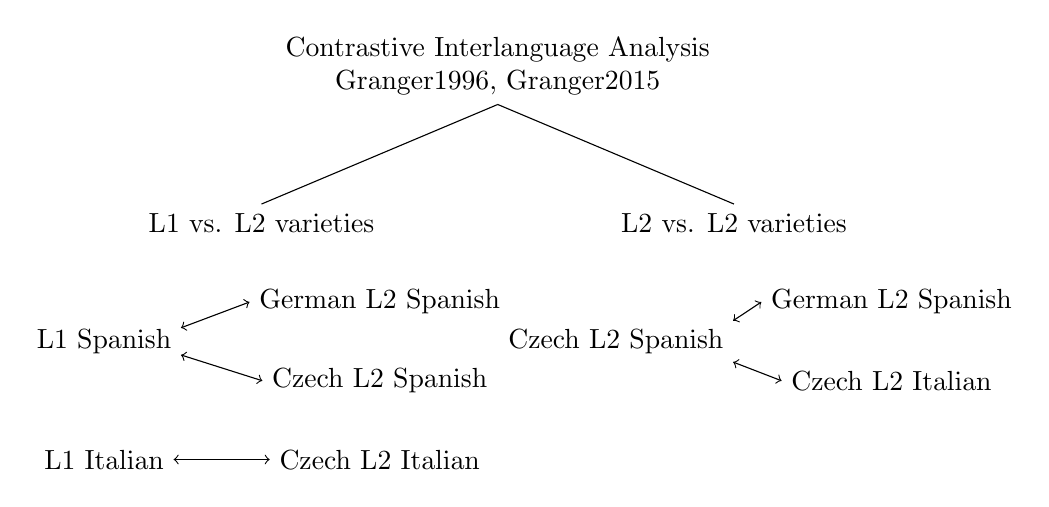
\begin{tikzpicture}[align=center, anchor=center]
\node(top) at (0,5) {Contrastive Interlanguage Analysis\\\citep{Granger1996, Granger2015}};
\node(12) at (-3,3) {L1 vs. L2 varieties};
\node(22) at (3,3) {L2 vs. L2 varieties};
\draw (top.south) -- (12.north);
\draw (top.south) -- (22.north);

\node(1sp) at (-5,1.5) {L1 Spanish};
\node(ge2) at (-1.5,2) {German L2 Spanish};
\node(cz2) at (-1.5,1) {Czech L2 Spanish};
\draw[<->] (1sp.10) -- (ge2.west);
\draw[<->] (1sp.350) -- (cz2.west);

\node(1it) at (-5,0) {L1 Italian};
\node(cz2it) at (-1.5,0) {Czech L2 Italian};
\draw[<->] (1it.east) -- (cz2it.west);

\node(cz2sp) at (1.5,1.5) {Czech L2 Spanish};
\node(ge2r) at (5,2) {German L2 Spanish};
\node(cz2r) at (5,1) {Czech L2 Italian};
\draw[<->] (cz2sp.10) -- (ge2r.west);
\draw[<->] (cz2sp.350) -- (cz2r.west);

\end{tikzpicture}
\caption{Varieties under study according to the \textit{Contrastive Interlanguage Analysis} (based on \citealt{Granger1996,Granger2015}).}
\label{fig:1:1}
\end{figure}

The first scenario involves a comparison of learner data with data from native speakers (L1 Italian vs. L2 Italian, L1 Spanish vs. L2 Spanish). In this instance, I provide basic information about the ways in which the four languages (L1 Spanish, L1 Italian, L1 German, L1 Czech) differ, on the basis of which hypotheses can be formulated. The second scenario includes an analysis of learners from two different language backgrounds (L2 Spanish with L1 Czech vs. L2 Spanish with L1 German). The last scenario examines differences between two different L2s produced by learners of one L1 background (L2 Italian with L1 Czech vs. L2 Spanish with L1 Czech).\footnote{One might note that the scenario “L2 Italian produced by L1 German learners” is lacking here. This is due to the COVID-19 pandemic, which did not allow to carry out the recordings. This L2 variety will be considered in future.} The contrast between all these varieties should clarify not only transferred phenomena but also common tendencies related to the acquisition of L2 intonation in general.


The third aim of the study is to discuss the results within the recently proposed \textit{L2 Intonation Learning theory} (LILt) \citep{Mennen2015}, a theoretical framework designed for intonation. The LILt is based on the Autosegmental-Metrical model of intonational phonology according to which languages differ in four dimensions: tonal inventory, phonetic realization of the tones, function of the tones and the frequency of their occurrence (see \sectref{sec:1.4} and \sectref{sec:2.4}). Here the study hopes to contribute to a better understanding of the interaction of these dimensions by evaluating the intonation patterns of L2 interlanguages in different types of sentence, including (non-)neutral statements, (non-)neutral yes/no questions, \mbox{(non-)}neutral wh-questions and vocatives.



And finally, the present study also contributes to the general discussion related to the modelling and transcribing of intonation, an issue that has been the subject of ongoing debate by applying ToBI (\textit{Tone and Break Indices}), a labelling system for tonal annotation (see \sectref{sec:2.2} and \sectref{sec:3.4.1}), and then discussing the strengths and limitations of this procedure.



The next section introduces various phenomena related to second language speech in general and highlights the key areas that seek to explain L2 behaviour, giving special attention to language transfer and the impact of the L1 on the L2. Based on different core concepts, preliminary questions and expectations related to this study will be formulated.


\section{Second language speech: Terminology and starting hypotheses}\label{sec:1.3}
\subsection{Core concepts}\label{sec:1.3.1}

As explained above, L2 speech refers to non-native production by an individual of a language that was acquired after that person had fully acquired (or nearly so) his/her native or first language(s) (L1).\footnote{The potential influence of another previously acquired L2 -- hence L2 to L3 transfer -- will not be covered in the present study, although the growing field of L3 acquisition has proved that such influences potentially play a role (e.g., \citealt{Odlin1989, CenozEtAl2001, HufeisenFouser2005, DeAngelis2007, Leung2009, WrembelEtAl2010, DeAngelisDewaele2011, GabrielGrünke2018}).} Previous research has looked at the phenomenon of non-native speech from two primary perspectives, one empirical-theoretical (see, e.g., \citealt{Hansen2006} and works cited therein) and the other empirical-didactic (see, e.g., \citealt{LightbownSpada2013}). Whereas the first perspective aims to explain the mechanisms of L2 acquisition as well as individual differences observed in L2 speech, the second one is more concerned with the pedagogical implications and possible strategies for pronunciation instruction in second language teaching. Within the course of the present work, I will focus especially on the main findings from the first area.


In order to understand second language speech and its mechanisms, it is important to first understand some general concepts in second language acquisition (SLA) (see, e.g., \citealt{Brown2000, GassSelinker2008, ColantoniEtAl2015, DerwingMunro2015, VanPattenBenati2015, AlonsoAlonso2018}). \citet[5--16]{TowellHawkins1994} recognize five core areas in explaining L2 behaviour, which will be defined and discussed briefly in turn. It is important to state at the outset that all these inter-related concepts are expected to be relevant for the acquisition of L2 intonation and for formulating the starting hypotheses (\sectref{sec:1.3.2}).



\subsubsection{Incompleteness}
Although in the course of their lives people never lose the ability to learn a new language, it has been widely assumed that after a certain age the majority of L2 learners differ from native speakers of that target language. However, so far there is no consensus in the research on exactly what that age is (see discussion of this topic in \sectref{sec:2.1.3}). \textit{Incompleteness} can be regarded as an L2 end-state grammar, that is, a state beyond which the grammar will not progress further. The end-state grammar characterizes a learner’s ultimate attainment and exhibits different degrees of native-like patterns (\citealt[5]{ColantoniEtAl2015}). Incompletely acquired properties, transfer phenomena or errors in the L2 may result in fossilization or an apparent “cessation of learning” \citep[457]{Odlin2003}, in which some non-native features become stable in a person’s individual way of speaking or writing. Foreign accent may be seen as a product of fossilized L2 pronunciation. The reasons behind the fossilization can be linguistic, neurolinguistic, socio-communicative or instructional in nature (see, e.g., \citealt{Sims1989, HanOdlin2005}). Moreover, \citet{Selinker1993} asserts that fossilization is a type of (predominantly) linguistic simplification that plays -- next to language transfer -- a central role in SLA. In syntax, for example, learners prefer SVO word order over the more complex cleft structures (see, e.g., \citealt{Schachter1988}), and in morphology, learners may simplify the “rich” verbal paradigm of a target language by using fewer or wrong forms independent of their L1 (see, e.g., \citealt{Montrul2011}).



\subsubsection{Cross-linguistic influence (CLI) or language transfer} 
This phenomenon involves all levels of language and is fairly consistently present in all learners. I will use CLI (see \citealt{SharwoodSmithKellerman1986}) and language transfer (see \citealt{Weinreich1953}) interchangeably here to refer to any “influence resulting from the similarities and differences between the target language and any other language that has been previously (and perhaps imperfectly) acquired” \citep[27]{Odlin1989}. Here we should distinguish between positive and negative transfer. \textit{Positive transfer} occurs when L1 and L2 share similarities and learners produce the target language in a native-like manner. \textit{Negative transfer}, on the other hand, occurs when features from the L1 are introduced inappropriately into the L2. Phenomena originating from negative transfer have generally been assumed to be of much greater interest for research purposes, no doubt because transferred dissimilarities are more easily perceived than similarities, though it has been argued (see, e.g., \citealt{Ringbom1987,Ringbom1992}) that positive transfer may affect second language acquisition even more than negative transfer. Differences between the languages at the (phonetic-)phonological level and the resulting (negative) transfer of L1 properties into the L2 contribute significantly to non-native speech.



\subsubsection{Developmental sequences}
This area refers to the fact that L2 learners do not acquire \textit{all} the properties of the L2 at once, since L2 acquisition -- similar to L1 acquisition -- undergoes several stages of development. This means that the learner’s perceptual and productive knowledge changes in the process of acquisition and (mostly) differs from the output we would expect from a native speaker (see, e.g., \citealt{Major1994}). In the theory of SLA this phenomenon is called \textit{interlanguage}, a term coined by \citealt{Selinker1972} (see also \citealt{Selinker1969}). Interlanguage is defined as a separate linguistic system -- an interim grammar between L1 and L2 -- which is “based on the observable output which results from a learner’s attempted production of a TL [target language] norm” \citep[214]{Selinker1972}. In the course of L2 acquisition, the learner develops different interlanguage grammars and strategies, in which further phenomena such as \textit{U-shaped learning patterns} or \textit{overgeneralizations} may emerge. A \textit{U-shaped learning pattern} (see, e.g., \citealt{Abrahamsson2003}) is a non-linear developmental phenomenon observed in individuals not only in L1 and L2 language acquisition but also in very different cognitive areas (see, e.g., \citealt{CarlucciEtAl2005}). As the name implies, learners perform correctly at the beginning of the acquisition process, then their skills descend over time before eventually becoming more accurate again. Errors in this process should not necessarily receive a negative interpretation. \citet{Gershkoff-StoweThelen2004}, who studied infant motor and language development, suggest that the regression in the U-shape development is just “apparent” and merely part of the ordinary mechanisms of change characterized by the collective dynamics of multiple, contingent processes.



One further developmental phenomenon typical of both L1 and L2 language acquisition is \textit{overgeneralization}. This refers to a type of error resulting from the inappropriate application of a rule or pattern and affects all domains of a language (see, e.g., \citealt{R.Ellis1994, WittekTomasello2002, Franceschina2005, GassSelinker2008, MontrulEtAl2010, LightbownSpada2013}). For example, children generally apply regular forms incorrectly to words that require irregular forms or endings (e.g., \textit{speaked} instead of \textit{spoke} in English; \textit{andé} instead of \textit{anduve} ‘I walked’ in Spanish; \textit{ich habe geschlaft} instead of \textit{ich habe geschlafen} ‘I slept’ in German, etc.). We can observe very similar morphological or morpho-syntactic errors in L2 learner productions too. In phonology, learners may overgeneralize segments and probably suprasegments too. For instance, I have observed that some L1 German learners of Spanish tend to pronounce the alveolar trill [r] in contexts where they should use the alveolar tap [ɾ] (e.g., <presente> *[presente] ‘present’). But note that this overgeneralization may actually indicate progress in the learner’s ability to produce the Spanish trill sound [r], which commonly causes difficulty for German native speakers. Overgeneralization can also be understood as a tendency to overshoot or exaggerate the target norm. For example, \citet{Gass1984} reported L1 Italian learners of English exaggerating the VOT English norm, thus pulling away from both native as well as target values (see also \citealt{Flege1980} for a similar tendency in L2 English VOT produced by Saudi Arabians). With respect to intonation, \citet{SantiagoDelais-Roussarie2015a} report L1 German and L1 Spanish learners of French who tend to overshoot final rises at the right edge of non-final clauses in L2 French. Similar overgeneralization of interrogative patterns has also been observed in L1 Italian learners of L2 (Peninsular) Spanish in \citet{GabrielKireva2014a}. As in the case of U-shaped learning, overgeneralization or exaggerating can be viewed positively as an important part of development: “[L]earners first identify \textit{that} there is something to learn and then work out the details, which in many cases involves the maximization of the features of the new element/contrast” \citep[394]{Gass1988}.



\subsubsection{Systematicity}
\begin{sloppypar}
This property is related to the growth in L2 knowledge across learners, which exhibits an interesting parallelism to L1 development. Previous research on different morphological and syntactic phenomena has demonstrated that the same stages or sequences of development can generally be found across different groups of L2 learners, even when they are distinguished by their ages, L1 backgrounds or conditions of exposure to the L2 (see \citealt[11--12]{TowellHawkins1994}). In L2 phonology research, evidence on such “universal” development is reported too. For example, \citegen{Carlisle2001} careful and detailed review of research on syllabic structure acquisition offers evidence that syllable universals have a strong influence on how L2 learners of various L1 backgrounds acquire such structures in different L2s (with the main claims including preference for CV syllables, more frequent modifications of longer margins, less deletion of more sonorous codas, more modifications of margins according to sonority principles, and modification of less preferred margins). Carlisle concludes that there is a “universal” systematic path of (phonological) development independent of L1 and/or the type of input. This does not mean, however, that L1 would not play any important role in the developmental sequences that appear in L2 phonology. As \citet[13]{Ioup1984} and later many others (e.g., \citealt{Shen1990, Wennerstrom1994}) have pointed out, “transfer is \textit{the} major influence on interlanguage phonology”, with a much greater impact here than on interlanguage syntax or other domains. To come back to the example of syllabic structure, Czech-speaking learners of German will have fewer difficulties with acquiring German consonant clusters than, for instance, L1 Spanish or L1 Italian learners. This is because Czech has more complex syllables and codas, whereas Spanish and Italian prefer CV syllables or syllables with simple codas. Hence, transfer processes clearly permit Czech learners to acquire German syllabic structure more rapidly. Also studies on the acquisition of word-stress by French-speaking learners of English (\citealt{Tremblay2008a,Tremblay2008b}, see also \citealt{TremblayOwens2010}) showed that the development of L2 prosodic representations is not random: most of the learners acquired the trochaic foot as they became more proficient in English \citep[168]{Tremblay2008a}. Nonetheless, in general terms more research on different language combinations and cross-linguistic comparisons is still necessary to enable us to explain which phenomena (if any) in prosodic development are universal and which are language-specific. Regarding L2 intonational development, we still lack research here, but see cited works in \sectref{sec:1.4.2}.
\end{sloppypar}


\subsubsection{Variability}\largerpage
This concept implies that L2 learners’ interlanguage systems change over time and go through different stages of variability. L2 learners may variably use two or more forms for a given construction or category. Intermediate speakers in particular can exhibit a very broad inventory of such variation in target sounds or \textit{approximation} attempts (see, e.g., \citealt{Beebe1984}) before they show stabilization in choice of the form. The interlanguage variability occurs either between learners (interlearner variability) or within the same learner (intralearner variability) and its degree is determined by different factors including L1 background, proficiency level, age of L2 learning, role of input and a range of personal reasons. \chapref{ch:2} (\sectref{sec:2.1}) will address all these factors in greater detail.



Similarly as in L1 acquisition, the performance mistakes do not necessarily reflect what L2 learners actually know (i.e., their competence). Indeed, one difficulty for a researcher is not merely to recognize whether a given speaker’s speech contains performance or competence errors (especially in terms of intonation), but also to determine what counts as an error in general (for a discussion on this topic, see, e.g., \citealt{Ringbom1987, GilquinDeCock2011}). When talking about an error in the present study, I will follow a working definition proposed by \citet[57]{DerwingMunro2015}, who define errors as “cases in which a speaker aims to produce an utterance, but as a result of a lack of full control over its segmental or suprasegmental structure, produces something else instead.” This “something else” is mostly a result of cross-linguistic influence. Moreover, while some production errors may be of temporary duration, others may continue over long periods and can lead to fossilization.


\subsection{Starting hypotheses}\label{sec:1.3.2}

Based on the main concepts in SLA presented above and the universal mechanisms of SLA as proposed in \citet{TowellHawkins1994}, the present study makes the following preliminary assumptions.

\begin{description}
\item[Incompleteness hypothesis:] According to this hypothesis, L2 grammar just approaches to the target language and L2 varieties will thus differ from the target languages. Since fossilization makes an important part of the “incomplete” acquisition, several related questions require an answer: What intonational features are candidates for fossilization in L2 speech and why? At what point does fossilization begin?

\item[CLI hypothesis:] It is expected that the learners will exhibit both positive and negative transfer of L1 features and these will be mixed with patterns of the target languages. But will transfer occur in all sentence types and with all tonal elements (pitch accents and boundary tones) in the same way?

\item[Developmental hypothesis:] It was reported that the degree of CLI depends on the stage of L2 development: as L2 development proceeds, L1 transfer effects diminish. The present study expects to find significant differences between intermediate and advanced learners. It is expected that advanced learners will more closely approximate the intonation patterns of the target language. Therefore, L1 Czech and L1 German advanced learners of Spanish should become more similar in their production than intermediate learners. In the same way, advanced learners of L2 Italian will more closely approximate the native-like patterns than intermediate learners. It is also expected that phenomena such as simplification and overgeneralization will arise as evidence of the acquisition strategies and the intonational development.

\item[Systematicity hypothesis:] This hypothesis states that the growth of L2 knowledge will be similar across learners, and similar types of interferences are expected. Another task regarding systematicity and development will be to consider which phenomena might be “universal” and which language-specific.

\item[Variability hypothesis:] The data on L2 intonation predict high (especially interlearner) variation. Though the strength of transfer can have various causes, the present study focuses on L1 background as a main factor and language proficiency as a secondary factor. Other factors such as, for example, the length of experience in a L2-speaking country, are left for the future (see also \sectref{sec:2.1}).
\end{description}

In addition to these basic hypotheses, several \textit{partial hypotheses} related to differences and similarities between L1 and L2 will be developed in the course of the present study. Before highlighting several problematic issues pertaining to the acquisition of L2 intonation and presenting the main findings of some case studies that have focused on L2 Spanish and L2 Italian intonation (\sectref{sec:1.4.2}), I will offer an overview of research concerned with language contact and change (\sectref{sec:1.4.1}). Based on the reported intonation deviations and prosodic transfer in these two areas, several generalizations about L2 behaviour in terms of intonation will be derived.

\section{Previous research on non-native intonation}\label{sec:1.4} %1.4 /
\subsection{L2 intonation in language contact studies}\label{sec:1.4.1}

Interference phenomena play a crucial role in the studies on language contact, which is a major factor in language change, including changes in the domain of phonology (see, e.g., \citealt{Weinreich1953, ThomasonKaufman1988, McMahon2004}). An important point for us here is that most distinctive sound patterns observed in many contact-induced varieties of Spanish and Italian can be seen as products of second-language pronunciation and cross-linguistic influence.


The Spanish language and its long-standing contact with different languages serves as an excellent illustration of diversification based on L1-L2 transfer. One example par excellence is Buenos Aires Spanish, called \textit{Porteño}, which features changes in the prosodic system that were probably triggered by a large Italian immigration in the second half of the 19th century and first third of the 20th (see  \citealt{VidaldeBattini1964, FontanelladeWeinberg1987, Nascimbene1988, Baily1999, Devoto2002}).\footnote{A large majority of Italian immigrants came from either the Piedmont or the South of Italy and spoke mostly regional varieties of Italian and/or Italo-Romance varieties, which were partly mutually unintelligible and led probably to the creation of a linguistic “Babel” (a mixture of these varieties and L2 Spanish).} Several studies devoted to the prosodic aspects of this modern Spanish variety provide empirical evidence that Italian and \textit{Porteño} share several similarities: the early alignment of F0 in prenuclear pitch accents, the final “long fall” in declaratives, the rising-falling boundary tone in yes/no questions and the use of emphatic tritonal pitch accents are the most cited features attributed to the Italian influence (see, e.g., \citealt{Kaisse2001, ColantoniGurlekian2004, GabrielEtAl2010,GabrielEtAl2011, FeldhausenEtAl2011, BenetEtAl2012, PeškováEtAl2012,PeškováEtAl2013}). Interestingly, comparable Italian traces and changes in the prosodic system have also been detected in the Occitan spoken in the Alpine valleys of northwestern Italy \citep{Sichel-BazinEtAl2015}, in the Catalan spoken in the Sardinian city of l’Alguer \citep{PrietoEtAl2015a}, in Tyrolean German \citep{Barker2005} or in the Spanish variety spoken in Mexican Chipilo, where immigrants from northern Italy (Veneto) settled (\citealt{BarnesMichnowicz2015}).



It is assumed that the typological closeness between Italian and Spanish possibly accelerated the creation of a new variety (\citealt[107]{ColantoniGurlekian2004}). Nevertheless, this does not mean that typologically distant languages cannot influence each other. Some examples can be found in Spanish dialects which were in contact with (sub-Saharan) African languages as a consequence of the Atlantic slave trade. By way of illustration, African-influenced intonation patterns have been observed in the vernacular speech of black communities in the Dominican Republic \citep{Megenney1982}. Megenney found that typical declaratives of this community end on a mid tone rather than a falling tone as in other Spanish dialects; this may neutralize the intonational differences between statements and questions. Though a direct influence of African languages on (Dominican) Spanish intonation is not very easy to demonstrate, the different-sounding Spanish dialect points to a possible African substrate impact on the Spanish superstrate. Similar African traces can also be found in the Afro-Iberian creole language \textit{Palenquero} (spoken in the Colombian village of San Basilio de Palenque), which displays a very unique intonation. \citet{HualdeSchwegler2008} show that all prenuclear stressed syllables receive high tones instead of the typical Spanish late peaks in posttonic syllables. A similar “sing-song” intonation and low-high tonal alternations have also been reported in the variety of Spanish spoken in Equatorial Guinea, a former Spanish colony, where Spanish is still a co-official language. The Bantu languages Spanish is in contact with in this area belong to tonal languages characterized by lexical high and low tones (see \citealt{Lipski2005,Lipski2010}). Another contact-induced Spanish dialect with “non-monolingual” intonation patterns is Peruvian Spanish \citep{ORourke2004}, in which (especially Quechua-dominant) bilingual speakers tend to produce prenuclear pitch accents with earlier peaks in the tonic syllable (see also \citealt{Buchholz2021} for Quechua-Spanish contact patterns). Differences in peak alignment have also been observed in Basque-Spanish bilinguals \citep{Elordieta2003} or Spanish-German bilingual children (\citealt{LleóEtAl2004, Lleó2016}).



Besides the above mentioned language contact situations, there are many further studies on intonation, examining, e.g., Yucatecan Spanish in contact with Maya in Mexico \citep{Uth2019}, Spanish-Guaraní contact in Argentina \citep{Colantoni2011} and Paraguay \citep{Pešková2022a}, Spanish-Portuguese contact in Spanish Olivenza \citep{Kireva2016}, Judeo-Spanish in contact with Bulgarian (\citealt{GabrielKireva2014b}), Cuban Spanish in contact with English and other Spanish dialects in Miami \citep{Alvord2006}, Spanish-Catalan contact in Mallorca \citep{Simonet2008} and in Catalonia (\citealt{GrünkeInProgress}). All these studies support the hypothesis that contact-induced changes significantly affect the intonational system (see also \citealt{FrotaPrieto2015} for such influences within other Romance languages; \citealt{Mencken1937} and \citealt{Romaine2001} for a brief remark on the intonation of Pennsylvania German English; \citealt{Grenoble2010} for intonational influences in Slavic languages; \citealt{Birkner2004} for influence of Portuguese in Brazilian German bilinguals; and many other examples).



With regard to contact-induced changes in (the regional varieties of) Italian, \citet{Cerruti2011},  \citet{GiliFivelaEtAl2015} -- among many others -- suggest prosodic influences from the contact with local vernaculars all over Italy. For example, the regional varieties of Italian spoken in Sardinia share intonational similarities (e.g., falling patterns in yes/no questions) with Sardinian \citep{VanrellEtAl2015}. In the same fashion,  \citet{RoseanoFernándezPlanas2019} report similarities between Friulian, and the regional Italian variety spoken in the town Tolmezzo in the autonomous Friuli-Venezia Giulia part of Italy (see also  \citealt{FernándezPlanasEtAl2017}). It should be added that although the Italian phonological system is known for being very heterogeneous,  \citet[196]{GiliFivelaEtAl2015} claim that stereotypical patterns, meaning “patterns shared by many (maybe all) varieties” do exist (e.g., the fall from a high pretonic syllable to a low tone in neutral statements or the early peak alignment used for contrastive-correction focus; see \chapref{ch:4}).



What do we learn from all these contact situations for the present study? First, they support the starting hypotheses formulated in \sectref{sec:1.3}. As we saw, intonation patterns undergo modifications through language contact, and CLI may accelerate such changes, which can significantly affect the prosodic system. Second, the heterogeneity resulting from language changes and development is patterned. Third, languages in contact do not show a one-to-one transfer, but rather the creation of mixed systems, “innovative hybrids” \citep{Lipski2010} or “fusion-like” patterns \citep{Queen2001} which derive from the contact environment. Hence, the interlanguages differ clearly from both the native language and the target language (see, e.g., \citealt{Tarone1987}) and not all deviations are necessarily due to interferences (see, e.g., \citealt{KielhöferJonekeit2018}).



Since intonational variation and change observed in contact language situations are connected with interlanguages, I expect similar behaviour and principles that govern changes in intonation and the mechanisms of the acquisition processes in my data too. This raises questions about the extent to which intonation is learnable, what patterns from the L1 are transferred into the L2, and, importantly, whether there are limitations on the transfer, and if so, where they are and why they exist.


\subsection{L2 intonation in SLA studies}\label{sec:1.4.2}

As yet, research in SLA on phonology and especially intonation is considerably limited when compared with other domains of language. Our growing knowledge in the field of L1 intonation especially during the last two decades has resulted in an increased interest in L2 intonation acquisition too. However, an overwhelming number of studies on non-native intonation concern L2 English produced by speakers with various language backgrounds (see, e.g., \citealt{Barlow1998, Gut2009, Mennen2007,Mennen2015, MennendeLeeuw2014, Puga2019,Puga2021} for overviews). Only a smaller number of studies are devoted to non-native intonation in L2 Spanish and L2 Italian, and -- to the best of my knowledge -- none of these studies have taken into account learners with L1 Czech. The aim of this section is to present a summary of the main current research findings with a focus on Spanish and Italian.

\begin{sloppypar}
Already  \citet[7]{NavarroTomás1948} remarked that intonation represents the “greatest stronghold” in the acquisition of a foreign language. One of the first em\-pir\-i\-cal\-ly-ori\-ent\-ed investigations of non-native Spanish intonation were carried out by \citet{Cantero1994} and \citet{CortésMoreno1998, CortésMoreno2001}, who offer preliminary descriptions of different (Peninsular) Spanish tonal contours and place the focus on didactical issues, which should allow the learners to gain not only linguistic but also communicative and intercultural competences. The nature of possible difficulties in learning intonation and its development are also taken into account. For example, Cortés Moreno reports interesting results for L2 Spanish produced by L1 Chinese learners, revealing that they acquire Spanish intonation in the following order: declarative sentences > wh-questions > yes/no questions > exclamatory (emphatic) sentences. This observation implies that the acquisition of intonation is constrained and indicates in which area intonational difficulties and deviations may occur. The broad explanation pursued by Cortés Moreno is that the acquisition hierarchy is due to both positive and negative transfer from L1.
\end{sloppypar}



More recently, \citet{AstrucVanrell2016} have contributed to the field with their study on the acquisition of politeness and intonation, which examines semi-spontaneous data produced by L1 English (beginning-level) learners of L2 Spanish. Based on acoustic analysis couched within the AM approach, they found out that the learners applied sociopragmatic knowledge and formulated pragmatically appropriate speech acts relatively well, but differed from Spanish natives in the distribution and frequency of tonal accents and their phonetic realisation. Other studies provide evidence that L1 transfer is an important factor in the production of L2 intonation (see, e.g., \citealt{Radel2008} for cross-linguistic influence in L2 Spanish declaratives and yes/no questions produced by L1 German learners; \citealt{GabrielKireva2014a} for “Italian” boundary tones in L2 Spanish yes/no questions; \citealt{JunEtAl2018} for difficulties in the phonetic implementation of the prenuclear rising F0 contours in L2 Spanish statements produced by L1 Korean learners; \citealt{vanMaastricht2018} for the acquisition of focus marking in L2 Spanish produced by L1 Dutch learners).



Another group of studies within the AM framework provide a window onto the development of L2 intonation by examining tonal patterns of L1 English native learners of different Spanish dialects in a study abroad context (e.g., \citealt{HenriksenEtAl2010} for the Spanish of León in Spain; \citealt{Trimble2013} for the Spanish of Mérida in Venezuela; \citealt{Craft2015} for Valencian Spanish; \citealt{Buck2016} for Salamanca Spanish in Spain; and  \citealt{MéndezSeijas2018} for the variety of Spanish spoken in Barcelona). These studies prove that learners increasingly approximate target-like intonation in the course of time, although not all exhibit significant changes. This general finding is important because it means that intonation is learnable and that learners approximate the variety they are exposed to. A further conclusion is that CLI remains present to different degrees and that learners do not attain native productions completely: avoidance of \textit{uptalk} (a high-rising terminal) in statements, later peak alignment of prenuclear pitch accents and different types of boundary tones represent a particular difficulty at least for L1 English learners. However, intonation development does not affect all phenomena in the same way and exhibits individual differences. For example,  \citet{MéndezSeijas2018} observed that whereas some learners improved their production of boundary tones after a five-week immersion experience (see also \citealt{Zárate-Sández2018}), they did not exhibit notable changes in prenuclear positions. Méndez Seijas offers an explanation for this within the \textit{L2 Intonation Learning theory} (see more below): fossilization in the peak alignment of prenuclear pitch accents occurs due to the perceptual similarities between Spanish and English and the fact that the contours in this position do not change meaning. In contrast, the drop of English \textit{uptalks} over time can be linked with the “strong semantic weight” involved. In other words, the learners are forced to acquire the target pattern of statements in Spanish (here the falling contour) properly because rising patterns can be confused with a question.



With regard to the research on L2 Italian intonation (see  \citealt{DevísHerraiz2008, DeMeoPettorino2012} and \citealt{Nicora2020} for overviews), we can organise the work done roughly into two main groups: studies that adopt the AM framework (e.g., \citealt{AvesaniEtAl2015, TurcoEtAl2015, NicoraEtAl2019}) and practice-oriented studies (e.g., \citealt{PettorinoEtAl2012, DeMarcoEtAl2014, Mocciaro2014, ViglianoEtAl2016}). Independently from the approach, most of the studies aim to highlight difficulties related to intonation learning, by providing contrastive analysis of Italian and different languages. They also provide evidence of developmental sequences that move towards native-like patterns according to the differences observed between proficiency levels that learners mostly achieved through formal instruction. Similarly to research on L2 Spanish intonation, studies on L2 Italian intonation demonstrate the relevance of L1 to non-native speech and support the prosodic transfer hypothesis (e.g.,  \citealt{DevísHerraiz2008,DevísHerraiz2011} for the acquisition of declaratives and interrogatives in L2 Italian produced by L1 Spanish speakers; \citealt{CroccoBaele2012} for the development of the phonetic implementation of the rises in yes/no questions by L1 (Belgian) Dutch learners; \citealt{Mocciaro2014} for the acquisition of Italian wh-questions and yes/no questions by L1 Vietnamese learners; \citealt{AvesaniEtAl2015} for the acquisition of givenness and focus marking in L2 Italian produced by L1 German learners and vice versa; \citealt{TurcoEtAl2015} for the polarity contrast in L2 Italian produced by L1 German and L1 Dutch learners; \citealt{VitaleEtAl2017} for yes/no questions in L2 Italian produced by L1 Chinese learners; and \citealt{NicoraEtAl2018} for Italian yes/no questions produced by L1 (Irish) English speakers). Furthermore, the works on L2 Italian place a special emphasis on teaching and learning Italian as a foreign language and offer several production/perception-based or imitation-based techniques that should help learners to obtain native-like intonation patterns. For example, the recent studies by \citet{NicoraEtAl2018, NicoraEtAl2019} demonstrate positive effects of a specific training in L1 Hiberno-English learners of Italian. The training consisted in raising prosodic awareness and contrastive L1-L2 analysis, imitation tasks, self-recordings and auto-corrections with the visual support of Praat software. The authors nicely show an improvement in two tested areas, lexical stress placement and intonational patterns of broad focus declaratives and information-seeking yes/no questions.



The present study attempts to generalize the main findings from the above-mentioned research on L2 Spanish and L2 Italian (see also \citealt{Mennen2007,Mennen2015} for further language combinations), which all report intonation cross-linguistic influence. The following key points will all be developed further in the course of the study:


\begin{itemize}
\sloppy
\item Intonational transfer is attested with both pitch accents and boundary tones in different types of sentence.

\item Phonological features of intonation are acquired earlier than the phonetic control of pitch.

\item Difficulties in the phonetic domain concern especially pitch alignment, pitch range and pitch timing.

\item Pragmatically marked structures are acquired later than neutral structures.

\item Patterns with a strong semantic weight are acquired earlier than patterns with no changes in meaning.

\item Patterns that exist in both L1 and L2 are acquired earlier than new patterns.

\item L2 intonation can be improved by appropriate learning\slash teaching techniques.

\item L2 intonation is full of interlearner variation and prosodic development is mostly individual.

\item L1 based-transferred and/or mixed interlanguage patterns undergo stabilization over time.
\end{itemize}

In order to test such L2 behaviour and to understand the learning mechanisms of L2 intonation, the present study will interpret the results within the recent -- and to the best of my knowledge -- so far only model designed for the acquisition of intonation in a second language: The \textit{L2 Intonation Learning theory} \citep{Mennen2015}. The LILt can be understood as a “working model […] that aims to account for the difficulties that L2 learners encounter in producing L2 intonation” \citep[171]{Mennen2015}. This model recognizes four dimensions, in which languages (may) differ and from which predictions on intonation deviations can be made: (1) the systemic dimension, which concerns the inventory and distribution of structural phonological elements, (2) the realisational dimension, which refers to the phonetic implementation of such elements, (3) the semantic dimension, which refers to the function or meaning of the elements; and (4) the frequency dimension, which refers to the frequency of use of the elements. Moreover, the LILt suggests that these intonation dimensions do not create the same amount of difficulty in L2 learning. The main goal is to explain the nature of these difficulties and to discover whether and how contrasts between L1 and L2 play a role in them. Expanding on L2 perception-based models for segmental speech learning (\sectref{sec:2.4}), the LILt also postulates that most intonation deviations and difficulties may be perceptually motivated and that the degree of perceptual similarity is determined by the semantic dimension. It also underlines that tonal contrasts must be controlled for in terms of position and context (all these aspects and further details on the LILt will be presented in \sectref{sec:2.4}). Basing on the previous research as well as the findings of the present study couched within the LILt, I will propose a \textit{Developmental L2 Intonation Hypothesis} (\sectref{sec:5.4}) which seeks to capture the “universal” characteristics of interlanguage intonation development independently of learners’ L1 backgrounds and L2. It is my hope to contribute with this study to the understanding of this still relatively underrepresented area of second language acquisition.

\section{Organisation of the study}\label{sec:1.5}  %1.5 /

The study is organised in six chapters. \chapref{ch:2} consists of four main sections which lay the theoretical foundation for the topic of the present research. First, the findings from both theoretical and empirical research on important factors shaping L2 speech are presented and discussed (\sectref{sec:2.1}). The following section (\sectref{sec:2.2}) offers a definition on intonation and talks about how the prosodic structure of spoken utterances can be modelled. Special focus is placed on the ToBI labelling system, grounded in the Autosegmental Metrical model of intonational phonology, which will be applied in the present study. In \sectref{sec:2.3}, I will compare the phonological systems of the languages under study, including their segmental and suprasegmental properties. The last section of the chapter turns to the models and theories that researchers have developed for the analysis of L2 speech. \citegen{Lado1957} \textit{Contrastive Analysis Hypothesis} and \citegen{Mennen2015} \textit{L2 Intonation Learning theory} are at the centre of attention here (\sectref{sec:2.4}). In order to answer the research questions that guide the present study, L1 and L2 data were collected by means of a production experiment with a total of sixty learners and twelve (Spanish and Italian) controls. A description of the experiment, its design (\sectref{sec:3.1}), participants (\sectref{sec:3.2}), experimental procedure (\sectref{sec:3.3}), intonational analysis and acoustic measurements (\sectref{sec:3.4}) are given in \chapref{ch:3}.

\chapref{ch:4} is the core of the study. It describes the main results on F0 contours in L2 Spanish and L2 Italian, produced by L1 Czech and L1 German learners. The chapter has five sections in accordance with the sentence types analysed: neutral statements (\sectref{sec:4.1}), non-neutral statements (\sectref{sec:4.2}), yes/no questions (\sectref{sec:4.3}), wh-questions (\sectref{sec:4.4}) and vocatives (\sectref{sec:4.5}). Every section begins with a contrastive analysis between L1 and L2, from which a series of CLI hypotheses are derived, then presents L2 outcomes providing illustrative examples of intonational contours and concludes with a summary and discussion.

\chapref{ch:5} offers an overall summary and general discussion of the most salient findings, which include the differences between L2 learner varieties (\sectref{sec:5.1}), the accuracy of L2 intonation patterns (\sectref{sec:5.2}), the deviations in four dimensions of intonation assumed in the LILt (\sectref{sec:5.3}) and issues related to the developmental sequences (\sectref{sec:5.4}). Concluding remarks, recommendations and future directions for research are stated in \chapref{ch:6}.

\chapter{Theoretical background}\label{ch:2}

The main objectives of this chapter are to define the key concepts of L2 speech acquisition, to give insight into a study of intonation, to compare sound systems of the languages under study and to discuss relevant theories and models in the light of an exhaustive review of the literature that is relevant to the present study. The first section (\sectref{sec:2.1}) deals with several important factors affecting L2 speech (L1 background, L2 proficiency level, age of learning, role of input, phonological awareness, personal variables and other influences) and presents a large discussion on this matter (\sectref{sec:2.1.1}--\sectref{sec:2.1.7}). The second section (\sectref{sec:2.2}) is devoted to the definition and modelling of the suprasegmental phenomenon -- intonation. It provides a detailed description of the Autosegmental-Metrical Model (AM model) (\sectref{sec:2.2.1}) and the Tones and Break Indices (ToBI) annotation system (\sectref{sec:2.2.2}), which are both crucial for the current study. In addition, I will offer a set of AM-based labels chosen for the analysis of the present L2 data (\sectref{sec:2.2.3}). The third section (\sectref{sec:2.3}) outlines and compares phonological systems of the languages under study, taking into account segmental (\sectref{sec:2.3.1}) as well as suprasegmental features and the prosodic typology of languages (\sectref{sec:2.3.2}). The last section of the chapter (\sectref{sec:2.4}) introduces and discusses several important models and techniques of L2 speech acquisition, placing a special focus on \citegen{Mennen2015} L2 Intonation Learning theory.

\section{Factors affecting L2 speech}\label{sec:2.1}

Since it is true that language is inherently variable, it is also true that L2 languages are full of target-like variation patterns \citep[272]{Regan2013}.  Interlanguage production (and perception) is very characteristic of inter-learner variability (differences between learners) and intra-learner variability (variability within the same learner). The present study will concentrate on two main learner-related sources of variability taken into account for explaining variation patterns in an L2: the \textit{L1 background} (Czech vs. German) and \textit{L2 proficiency} (intermediate level vs. advanced level). My starting point is a very general assumption that the first language plays a key role in L2 speech (see, e.g., \citealt{Suter1976}). For example, it is not difficult for a native speaker to distinguish among Czech, Italian, Spanish and German accents in English.\footnote{There are two interesting online archives for listening to different accents in (L2) English: the \textit{International Dialects of English Archive} \citep{Meier1998} and the \textit{Speech Accent Archive} \citep{Weinberger2015}. Equivalent resources for L2 Spanish and L2 Italian do not exist, although some first steps have been made in this regard for Spanish (see, for example, the IFEC corpus project -- \textit{(Inter-)Fonología del Español Contemporáneo} -- presented in \chapref{ch:3}).} The first factor (\sectref{sec:2.1.1}) should elucidate production errors and interferences and explain the role of L1 in L2 speech in general. The second factor (\sectref{sec:2.1.2}) should explain whether errors attributable to \textit{transfer} decrease in more advanced learners and how the developmental sequences (may) change over time. It is suggested that with regard to language level, Czech and German learners of an advanced level should become more similar in their L2 Spanish than those of an intermediate level. In a similar way, it is to be expected that intermediate L2 Italian learners (L1 Czech) will resemble intermediate L2 Spanish learners (L1 Czech) and that the advanced groups will present more different intonational patterns. In the following sections, some other traditional factors asserted to affect L2 speech such as age of acquisition, the role of input, phonological awareness, gender and personal factors will also be reviewed (\sectref{sec:2.1.3}--\sectref{sec:2.1.7}). As we will see, there are several disagreements and even contradictory conclusions regarding the effect of different factors, which makes understanding of the interlanguage somewhat puzzling (for overviews and discussion see, e.g., \citealt{PiskeEtAl2001, ColantoniEtAl2015, DerwingMunro2015}). For example, whereas \citet[201]{PiskeEtAl2001} report “little evidence that amount of formal instruction as such affects degree of L2 foreign accent”, the majority of the studies reviewed by \citet{DerwingMunro2015} show that formal instruction such as specific training techniques yielded positive results in L2 accuracy. The reasons for the (partly) conflicting findings may be the study of different languages, examination of different phenomena, application of different experimental methods and measurements, or the complex nature of the L2 speech. In spite of several opposite and ambiguous results, it is, however, of utmost importance to control for different variables (see \citealt[5]{ColantoniEtAl2015}) because they can be very useful for the latter interpretation of the data and for gaining a deeper insight into the phenomenon under study.

\subsection{L1 background}\label{sec:2.1.1}\largerpage[2]

As already presented in the \textit{Introduction}, L2 speech is characterized by a phenomenon denoted as cross-linguistic influence (CLI), language transfer or interference, which has an impact on all aspects of segmental and suprasegmental phonology. CLI or language transfer refers to the fact that L2 learners use L1 categories in their L2 production as well as their L2 perception (e.g., \citealt{Gass1984,Gass1996, Odlin1989,Odlin2003, Selinker1993, ColantoniEtAl2015}). One of the main reasons for this is that L2 learners mostly concentrate on meaning rather than form and because they are not starting from true “zero” in linguistic terms and therefore require “the overriding of the pre-existing L1 neural connections” (\citealt[90]{Kivistö-deSouza2015}; see \citealt{N.C.Ellis2002} and \citealt{R.Ellis2009} for a discussion on the relationship between the SLA theory and the neuroscience of learning and memory). It is thus reasonable to assume that the L1 background is the main determinant of L2 speech.


It is important to keep in mind that \textit{accentedness} in L2 (the extent to which a listener judges L2 speech according to the native speaker norm, see, e.g., \citealt{Piske2008}) is not the same as \textit{identification} of the speaker (recognition of where the L2 speaker is from, see, e.g., \citealt{KollyDellwo2013}). We can generally make a good guess about where the speaker comes from. So, for example, one Czech and one German speaker may be both evaluated to have a very weak foreign accent, but we may be able to hear differences between them and very possibly say who is German and who is Czech. If the influence of L1 is expected, the following questions may arise: \textit{Do German learners of Spanish differ substantially from Czech learners of Spanish in terms of intonation? Are there any tonal features typical of German or Czech learners in particular? If so, do we find the same features in two different target languages (Italian and Spanish) produced by learners coming from the same L1 background?} These and other questions will accompany this study. In the following sections, I will discuss some traditional factors claimed to affect L2 speech. Specific hypotheses of the present study based on cross-linguistic influence will be formulated in \chapref{ch:4}.


\subsection{L2 proficiency level}\label{sec:2.1.2}\largerpage[2]

Second language proficiency or the ability of an individual to speak and perform in an L2 is another factor expected to explain the variability observed in L2. For example, the study by \citet{CroccoBaele2012} on yes/no questions in L2 Italian by L1 Dutch speakers has shown that advanced learners produce more native-like patterns compared with less experienced learners. In a similar way, a longitudinal study by \citet{MennenEtAl2010} has shown that Italian and Punjabi learners of English make certain improvements in L2 intonation (e.g., the use of certain target-like patterns) over the course of their stay in the host country.


Due to the fact that the present research is not longitudinal in nature, its main idea is to compare intermediate (B level) and advanced (C level) learners in order to find out whether there are any differences between the two groups and whether there is positive movement towards a native-like production in terms of intonation. Such a cross-sectional approach has been to date the most common way to account for L2 development.



The proficiency level of the learners examined in the present study was determined according to the CEFR guideline (\citealt{CEFR2001,CEFR2011, CEFR2018}), which describes the achievements of learners of L2 languages and is commonly used across Europe, including Germany and the Czech Republic. All the participants of the present study self-reported their foreign language proficiency levels in accordance with the courses they were attending (or had recently finished) at the time of the experiment. No specific tests for measurements of participants’ phonological or other linguistic competences were carried out, but the learners were asked to answer a set of predetermined questions in a semi-directed interview (see \sectref{sec:3.2} for details), the aim of which was to detect, among other things, their explicit L2 phonological awareness (see \sectref{sec:2.1.6}). It should be pointed out that the determination of participants’ levels within the “traditional” proficiency frameworks (and the present study too) is actually based on grammar, vocabulary, oral and written expression and overall communication skills rather than on phonological competence. The target skills for spoken interaction and production as stipulated by the CEFR essentially focus on (speech) intelligibility, “the most fundamental characteristic of successful oral communication” (\citealt[1]{DerwingMunro2015}). \tabref{tab:2.1} offers a full description of spoken competences of learners at B and C levels as proposed in \citet{CEFR2018}.


\begin{table}
\begin{tabularx}{\textwidth}{lX}
      \lsptoprule
      \multicolumn{2}{l}{Independent (intermediate) users}\\\midrule
      B1 & I can connect phrases in a simple way in order to describe experiences and events, my dreams, hopes and ambitions. I can briefly give reasons and explanations for opinions and plans. I can narrate a story or relate the plot of a book or film and describe my reactions.\\
      B2 & I can present clear, detailed descriptions on a wide range of subjects related to my field of interest. I can explain a viewpoint on a topical issue giving the advantages and disadvantages of various options.\\\midrule
      \multicolumn{2}{l}{Proficient (advanced) users}\\\midrule
      C1 & I can present clear, detailed descriptions of complex subjects integrating sub-themes, developing particular points and rounding off with an appropriate conclusion.\\ 
      C2 & I can present a clear, smoothly flowing description or argument in a style appropriate to the context and with an effective logical structure which helps the recipient to notice and remember significant points.\\
      \lspbottomrule
  \end{tabularx}
\caption{Spoken skills for levels B and C according to the \citet{CEFR2018}.}
\label{tab:2.1}
\end{table}

In real life and many language courses, pronunciation still plays a relatively secondary role in an individual’s language proficiency. And as \citet[47]{CEFR2018} admits, “[p]honology had been the least successful scale developed in the research behind the original descriptors.” Nevertheless, this does not mean that phonology is completely ignored in the CEFR proposals. Let us here make a short digression to look at the latest proposals in this regard and start with the illustrative descriptor scale proposed already in 2001 for the assessment of foreign language proficiency (\tabref{tab:2.2}).

\begin{table}
	\begin{tabularx}{\textwidth}{lX}
		\lsptoprule
		\multicolumn{2}{l}{Independent (intermediate) users}\\\midrule
		{B1} & Pronunciation is clearly intelligible even if a foreign accent is sometimes evident and occasional mispronunciations occur.\\
	    {B2} & Has a clear, natural pronunciation and intonation.\\\midrule
	    \multicolumn{2}{l}{Proficient (advanced) users}\\\midrule
	    {C1} & Can vary intonation and place sentence stress correctly in order to express finer shades of meaning.\\
	    {C2} & {\itshape No descriptor available}\\
		\lspbottomrule
	\end{tabularx}
	\caption{Phonology scale according to the \citet{CEFR2001}.}
	\label{tab:2.2}
\end{table}

Although this proposed scale for phonological skills is transparent, comprehensive and broad enough to capture new directions in L2 learning and teaching, it has not gained widespread acceptance, for three main reasons. First, it is oriented (implicitly) around the native speaker norm. Second, its main focus is on intelligibility (“clearly intelligible”, “a clear pronunciation”, “finer shades of meaning”) and comprehensibility (“can be understood”) rather than on any concrete pronunciation skills (for example, intonation skills are mentioned first at the B2 level, even though this aspect is present in the target language from the very beginning of acquisition, in contrast to certain vocabulary or grammatical categories). And third, the treatment of foreign accent does not reflect reality. As we have noted, a foreign accent seems to be in effect “tolerated” until the B1 level; from this level on learners are presumed to have mastered L2 pronunciation “perfectly”. Notice that there is no descriptor available for C2 at all, which again implies that phonological skills must be fully acquired not later than the C1 level, which is quite an unrealistic ambition. This is also critical because a foreign accent is very negatively seen at this level and from research we know that even highly advanced C2 speakers still may have a foreign accent. In an update, the CEFR \textit{Phonology} sub-project (\citealt{Piccardo2016, CEFR2018}) conducted various validation phases in relation to other new scales described below, with over 250 informants involved in each phase, and based on their results proposed a new phonological skills rubric for \citealt{CEFR2018} (\tabref{tab:2.3a}). This recent proposal is more extensive and comprises besides the overall phonological control two other core areas: sound recognition and articulation and prosodic features (including intonation, stress and rhythm). I present only the first and the last area here.\largerpage

\begin{table}
	\caption{Overall phonological control according to \citealt{CEFR2018}.}
	\label{tab:2.3a}
	\begin{tabularx}{\textwidth}{lX}
		\lsptoprule
		\multicolumn{2}{l}{{Independent (intermediate) users}}\\\midrule
		{B1} & Pronunciation is generally intelligible; can approximate intonation and stress at both utterance and word levels. Accent is generally influenced by other language(s) he/she speaks, and this may occasionally affect intelligibility.\\
		{B2} & Can generally use appropriate intonation, place stress correctly and articulate individual sounds clearly.
		
		Accent tends to be influenced by other language(s) he\slash she speaks, but has little or no effect on intelligibility.\\\midrule
		\multicolumn{2}{l}{{Proficient (advanced) users}}\\\midrule
		{C1} & Can employ the full range of phonological features in the target language with sufficient control to ensure intelligibility throughout.
		
		Can articulate virtually all the sounds of the target language; some features of accent retained from other language(s) may be noticeable, but they do not affect intelligibility at all.\\
		{C2} & Can employ the full range of phonological features in the target language with a high level of control -- including prosodic features such as word and sentence stress, rhythm and intonation -- so that the finer points of his/her message are clear and precise.
		
		Intelligibility and effective conveyance and enhancement of meaning are not affected in any way by features of accent that may be retained from other language(s).\\
		\lspbottomrule
	\end{tabularx}
\end{table}

\begin{table}
	\caption{Phonology control (prosodic features) according to \citealt{CEFR2018}}
	\label{tab:2.3b}
	\begin{tabularx}{\textwidth}{lX}
		\lsptoprule
		\multicolumn{2}{l}{{Independent (intermediate) users}}\\\midrule
		B1 & Can convey his/her message in an intelligible way in spite of a strong influence on stress, intonation and/or rhythm from other language(s) he/she speaks.\\
		B2 & Can employ prosodic features (e.g. stress, intonation, rhythm) to support the message he/she intends to convey, though with some influence from other languages he/she speaks.\\\midrule
		\multicolumn{2}{l}{{Proficient (advanced) users}}\\\midrule
		C1 & Can produce smooth, intelligible spoken discourse with only occasional lapses in control of stress, rhythm and/or intonation, which do not affect intelligibility or effectiveness. Can vary intonation and place sentence stress correctly in order to express precisely what he/she means to say.\\
		C2 & Can exploit prosodic features (e.g. stress, rhythm and intonation) appropriately and effectively in order to convey finer shades of meaning (e.g. to differentiate and emphasise). \\
		\lspbottomrule
	\end{tabularx}
\end{table}

The main difference with regard to the earlier proposal is that foreign accent is not completely excluded at the higher levels and it is not negatively perceived as long as it does not impede clarity and intelligibility. Today, the majority of experts agree that the \textit{Intelligibility Principle} (in terms of \citealt{Levis2005}) is more appropriate than \textit{nativeness} as a basic orientation to pronunciation instruction (see, e.g., \citealt{Piccardo2016, DerwingMunro2015}). This does not mean, however, that pronunciation is of little importance. Regarding the phenomenon under study here, learners at the B levels should use \textit{appropriate} intonation in order to “support message correctly” and those at the C levels should be able to use intonation \textit{appropriately} and \textit{effectively} in order to “convey finer shades of meaning”. Although this latest proposal is important, in my opinion, it is still very general and lacks information on what intonation parameters should be acquired exactly. Based on the findings of the present study, I will later offer a preliminary scheme on intonation scale or skills that can be integrated into the \textit{Phonology control} within the CEFR (see \chapref{ch:5}, \sectref{sec:5.2.1}). On the other hand, the particular strength of the proposal is that phonological skills, which were based on observations of L2 speakers with different L1 backgrounds, cover various phonetic and phonological phenomena and are not exclusively oriented around the native norm. That said, however, it should not be forgotten that the CEFR proposal is strongly Anglocentric as it was developed according to the \textit{lingua franca} English. Hence, the prosodic typology and prosodic systems of the individual target languages as well as issues such as the distance between the L1 and the target language are not taken into account here. It also raises the question as to how to implement such phonological assessment in language courses, which would imply a need to develop materials for both learners and teachers, to say nothing of the possible revising of language policy documents and teacher education in general \citep{Piccardo2016}.


Finally, it should be pointed out that the observations made by the new CEFR phonological assessment tool show that there are differences between the two levels (B and C) in terms of prosody; and, hence, a comparison of these two groups is appropriate for the aims of the present study. Of course, we shall not forget that the degree of foreign accent may be affected by further factors; some of them will be presented in the following sections. Moreover, \citet{MunroDerwing1995} showed that accentedness and intelligibility are partially independent. This leads to the question as to whether there are some common developmental mechanisms or whether and how phonological competence depends on other skills.


\subsection{Age of L2 learning \textup{(AOL)}}\label{sec:2.1.3}

It has been widely observed that accent-free speech in L2 is very difficult to attain and that late L2 learners usually tend to have a stronger degree of foreign accent than early L2 learners. \citet{PiskeEtAl2001} discuss the impact of the age of L2 learning (AOL) on the degree of foreign accent in their detailed review of the previous research on this factor (see also \citealt{ColantoniEtAl2015, DerwingMunro2015, Piske2017}, and more recently \citealt{FlegeBohn2021} for further readings). They cite many studies that have reported a positive effect of AOL, but they underline that such results may be only a byproduct of the interaction of different factors at the same time (such as the role of quantity and quality of input, length of residence or experience in an L2-speaking country, amount of L1, personal motivation, specific aptitudes, etc.). Although a majority of the previous studies agree on the view that “the earlier the better”, there is no common consensus on the age at which a truly native-like accent can be attained (if at all), and whether L2 speech learning is subject to some “critical period” (CP), in other words, whether and to what extent the ability to acquire language is biologically linked to age. According to \citegen{Lenneberg1967} \textit{Critical Period Hypothesis} (CPH) (see also \citealt{PenfieldRoberts1959}), attainment is not possible for learners who begin with L2 acquisition after puberty. The CP is thus assumed to end between ages 10--13 or at most at 15 years of age, due to the functional (re)organisation of neuropsychological systems and maturational changes in the brain that emerge around puberty (see, e.g., \citealt{Lamendella1977}). However, many subsequent studies have reported that nativelikeness is still possible after puberty, although only in a limited number of cases (see, e.g., \citealt{Birdsong2007}), and that not all early L2 learners are accent-free, even if they start to learn the target language at the age of six or even earlier (see, e.g., \citealt{Thompson1991}). In sum, the concept of a critical period has appeared rather untenable and the conclusions offered by many studies reveal that other linguistic, cognitive and social factors are involved in the language learning process and explain the advantage of age in it (see, e.g., \citealt{BialystokHakuta1999, Birdsong1999, LoewenReinders2011, FlegeBohn2021}, among many others).


It is important to add that many studies cited in \citet{PiskeEtAl2001} examined L2 speech produced by immigrants, who moved to an L2-speaking environment at different ages. In the present study, we deal with another situation. I examine speakers who started to learn L2 in a formal setting in their own home country. Moreover, the majority of the L2 participants started to learn the language after puberty, on average at the age of 17 (Czech learners) or 18 (German learners). This is also because English is mostly the first foreign language taught in both Germany and the Czech Republic. All the L2 learners were asked about their AOL. Interestingly, many of them reported differences between the age of first exposure and age when they “really” started to learn their L2 (see also \citealt{Piller2002}). For example, one participant commented on the AOL in the following way: “I had Spanish for the first time when I was 14, but only for a short time. I started to learn it properly at university when I was 19.” For the purpose of maintaining the uniformity of this factor between the speakers, the present study determines the very first exposure of the language as a criterion for the age of L2 learning (AOL) (see \sectref{sec:3.2} for details).


\subsection{Role of input}\label{sec:2.1.4} %2.1.4 /

As outlined in \sectref{sec:2.1.2}, the development of language proficiency is a gradual process which is closely linked to the input, i.e., to the ambient spoken and written language to which learners are exposed (\citealt[5]{ColantoniEtAl2015}). Input quantity, input quality and input modality have been reported to show significant consequences for L2 speech (see, e.g., \citealt{PiskeEtAl2001, ColantoniEtAl2015, DerwingMunro2015} for overviews). Some studies have purported that the factor \textit{length of residence} (LOR) in an L2-speaking environment has one of the most ameliorative effects on L2 performance (see, e.g., \citealt{AsherGarcía1969, PurcellSuter1980, FlegeEtAl1997, FlegeFletcher1992, HenriksenEtAl2010}). This can be explained by the fact that in such a context both input quantity (the amount of TL a learner receives) and input quality (a learner is -- in an ideal case -- surrounded predominantly by native speakers) are superior to what is present in standard language courses in the speaker’s home country. \citet{DerwingMunro2015} compared a total of thirteen studies on the effects of LOR on L2 pronunciation and/or perception and found out that whereas four studies reported no significant effect and two a mixed effect, seven studies showed a significant effect on L2 accuracy. In a similar way, the factor \textit{language use} (how many hours learners speak L2 a day/week) as a predictor of degree of L2 foreign accent showed many discrepancies in the outcomes of different studies (see also \citealt{PiskeEtAl2001}). \citet[39]{DerwingMunro2015} conclude that the observed contradictions among the studies are due to the complexity of the whole phenomenon and the interaction among several further factors at the same time. For example, \citet{FreedEtAl2004} showed that learners who acquired a foreign language through (domestic) immersion programs and techniques performed much better than learners who studied at home or who experienced a period of study abroad with possible interaction within the local L1 speech community.


Another factor linked to the role of input is \textit{formal instruction} (see also \sectref{sec:2.1.5}). Especially, different training techniques have been shown to have an important effect not only on L2 production accuracy but also on L2 perception (see, e.g., \citealt{Henning1966, MacdonaldEtAl1994, BongaertsEtAl1997, BradlowEtAl1997, Missaglia1999, DerwingEtAl1998, Moyer1999, WangMunro2004, IversonEtAl2005, TannerLandon2009, SaitoLyster2012}). Interestingly, many studies report that prosody-centred training has the strongest (positive) effect on L2 speech, where intonation plays a crucial role in both comprehensibility and intelligibility (e.g., \citealt{deBotMailfert1982, deBot1983, WeltensdeBot1984, DerwingRossiter2003, LevisPickering2004, Lengeris2012}).\footnote{As explained above, \textit{comprehensibility} refers to “the amount of effort that must be put in to understanding speech”, whereas \textit{intelligibility} refers to the clear pronunciation “so that listeners can understand the speaker’s intended message” (\citealt[1 and 3]{DerwingMunro2015}).} This shows how important prosody and especially intonation are for L2 learning (and teaching too). For example, \citet{LevisPickering2004} used speech-visualizing technology and demonstrated improvement in perception and production of intonation patterns in L2 English as well as an increase in sensitivity to pitch movement. A positive result of intensive perception-production prosodic training in the production of L2 Italian yes/no questions by English learners was reported recently also in \citet{NicoraEtAl2018} and in other studies on L2 Italian intonation (see \chapref{ch:1}, \sectref{sec:1.4.2}). Another recent study by \citet{Kushch2018} has shown that embodied training can positively influence both intonation and pronunciation in L2. In sum, many studies demonstrate that appropriate training is crucial for the development of phonological\slash pragmatic awareness in L2 and the improvement of learners’ competences in L2 speech.


\subsection{Phonological awareness in L2}\label{sec:2.1.5}

According to the so-called \textit{noticing hypothesis} coined by \citet{Schmidt1990}, noticing is the essential starting point for L2 acquisition, and awareness (through attention) is in turn essential for noticing (see also \citealt{Schmidt1993}). As we will see later, both awareness and noticing of intonation seem to be to a very large degree implicit. When we start to learn a new foreign language, we are usually taught first how its pronunciation system functions. We are made aware of certain segments (consonants and vowels) which do not exist in our language (e.g., the sound /y/ does not exist in Italian but in German) or which are very different or difficult to pronounce (e.g., the differences in \textit{r-}pronunciation between German and Spanish). The “wrong” pronunciation of sounds can significantly influence perception of them by natives. Surprisingly, explicit knowledge about the exact pronunciation rules of L2 as well as L1 remains still very limited for many learners (unless they undertake specific phonetic or phonological training). On the other hand, spotting foreign and regional or social accents usually does not require any special effort. According to \citet[42]{Moyer2004}, the pronunciation is an aspect of linguistic ability that is “psychologically loaded” and “inherently associated with identity” because it allows the speaker to be identified as either native or non-native. This means that we have both explicit and implicit knowledge not only about the target language but also about our L1. Thus far, research has focused mainly on phonological awareness in L1 and its relation to literacy achievement (e.g., \citealt{BradleyBryant1983, OakhillKyle2000, CunninghamCarroll2015}), and phonological awareness in L2 has been less explored (e.g., \citealt{GarcíaLecumberri2001, RamírezVerdugo2006, KennedyTrofimovich2010, Kivistö-deSouza2015}). Phonological awareness in L2 is understood as “knowledge about the target language phonological system at the segmental, prosodic and phonotactic domains, most of which is not available for conscious reflection or verbalization” (\citealt[105]{Kivistö-deSouza2015}). \citet{Kivistö-deSouza2015} includes within phonological awareness knowledge of both, contrastive units (phonemes) and non-contrastive units (allophones). This is important because L2 learners may be aware of phenomena, which are contrastive, and unaware of phenomena, which are not contrastive, or vice versa. Moreover, she assumes that L2 learners possess mostly limited (if any) \textit{declarative} (explicit) knowledge about the rules in L2 pronunciation, whereas all of them have \textit{proceduralized} (implicit or intuitive) knowledge about these rules. The relative amount of explicit vs. implicit knowledge varies from speaker to speaker and may be related to other factors. The relationship between these two areas is depicted schematically in \figref{fig:2.1}.



\begin{figure}
%%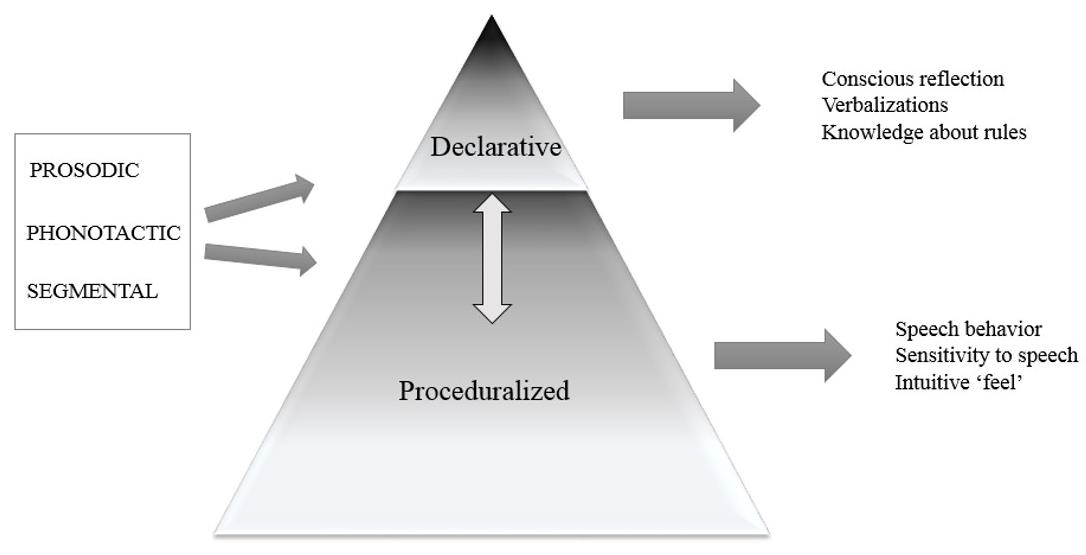
\includegraphics[width=\textwidth]{figures/a02HabilTheory-img002.png}
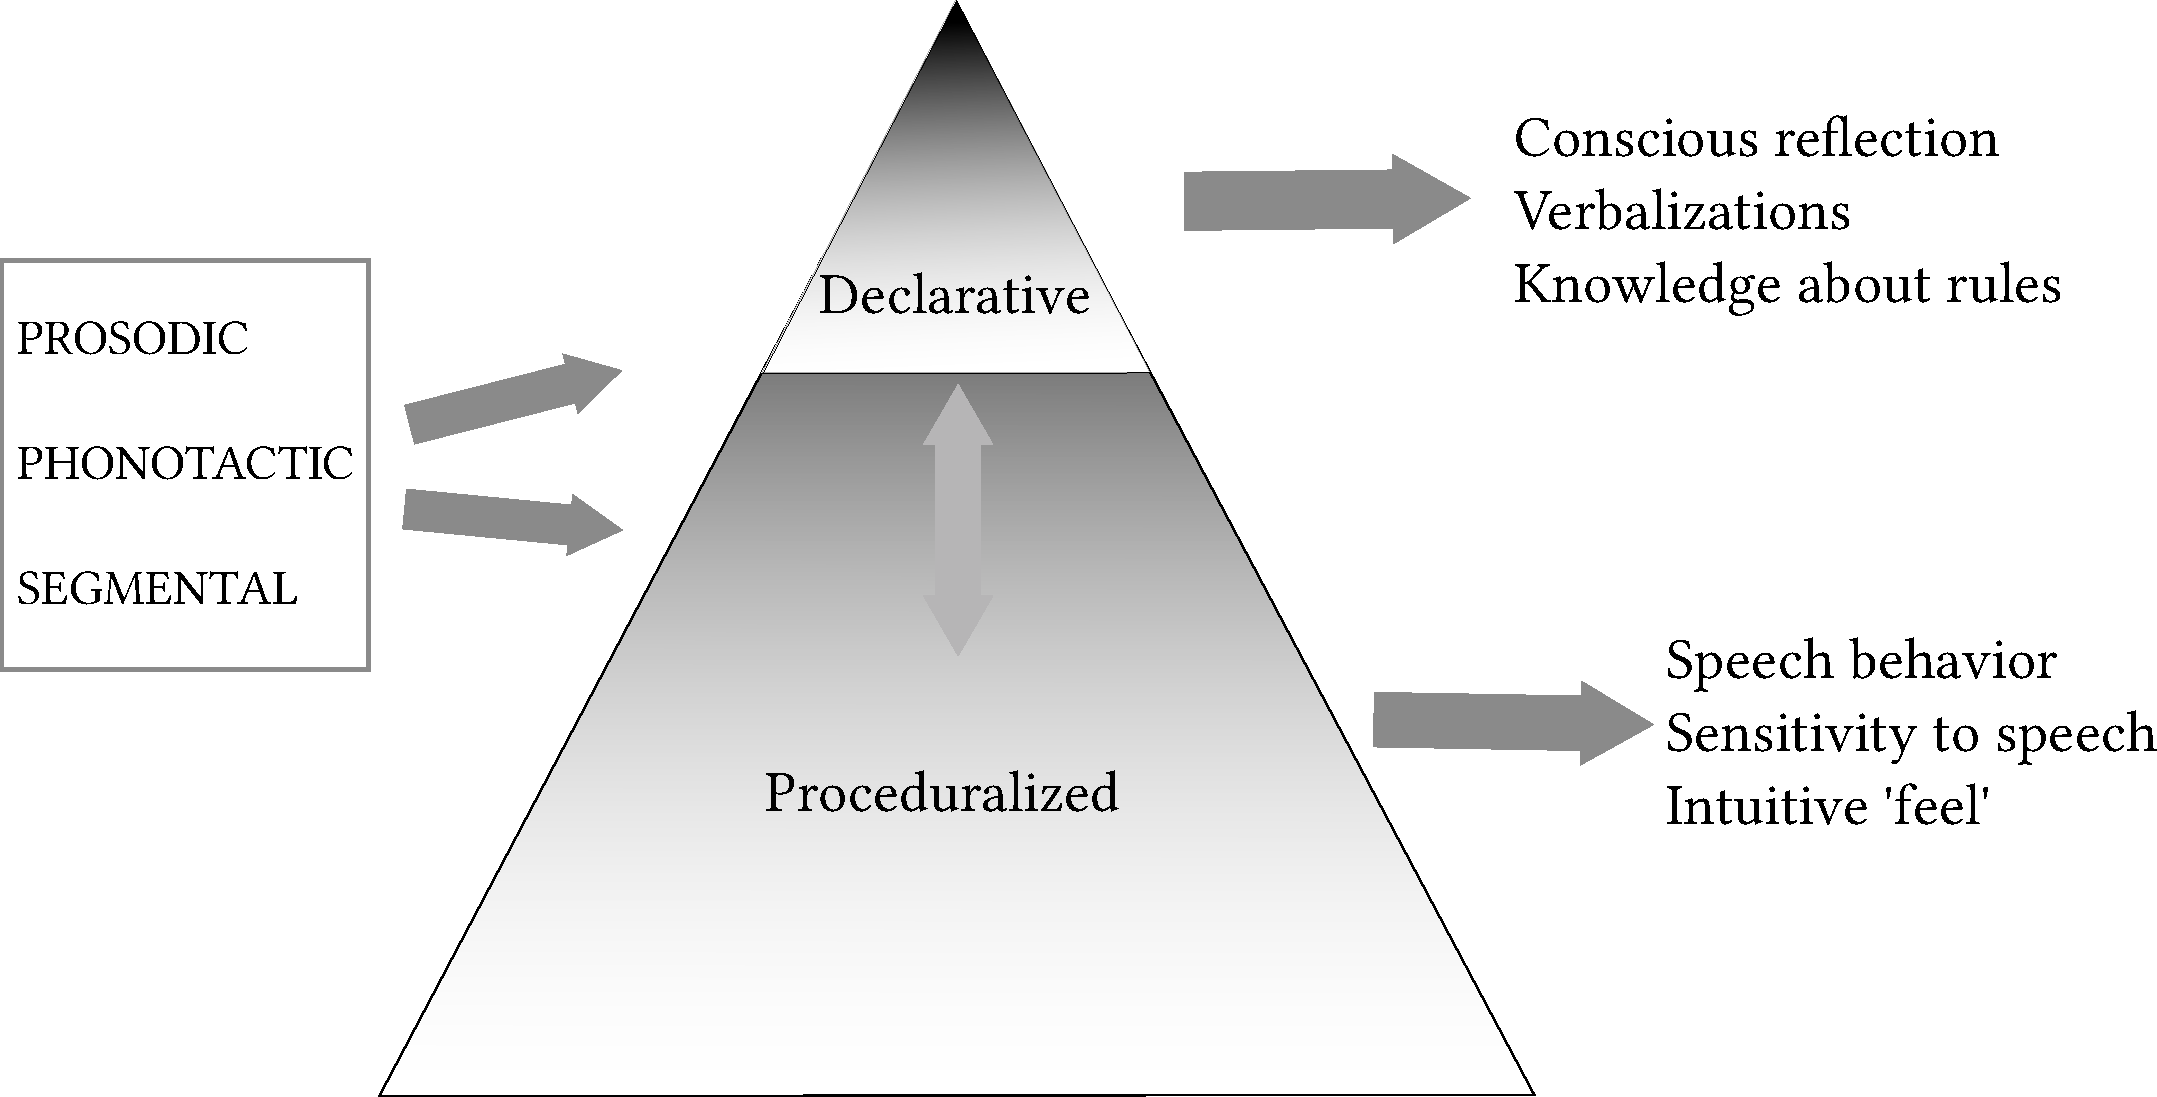
\includegraphics[width=\textwidth]{figures/a02HabilTheory-img002.pdf}
\caption{Phonological awareness in L2 according to \citet[106]{Kivistö-deSouza2015}.}
\label{fig:2.1}
\end{figure}

As already noted in the previous section, better formal instruction implies higher phonological awareness and that in turn leads to a better performance and L2 production accuracy (see, e.g., \citealt{MacKayEtAl2001, Piske2008, KennedyTrofimovich2010, Kivistö-deSouza2017}). \textit{Better} formal instruction means an explicit pronunciation instruction, involving special training in the perception and production of L2 segments as well as suprasegments.


Although the present study did not conduct any experiment in order to test and measure phonological awareness systematically across participants, the L2 learners were asked about their personal difficulties in L2 pronunciation as well as about differences between Spanish/Italian and their L1s in the semi-directed conversation conducted (see \chapref{ch:3}). The aim was to access the \textit{explicit} segmental as well as suprasegmental awareness in their L2 and to find out what sort of formal instruction they had got in terms of pronunciation. The learners were asked to answer the following two questions: \textit{What sounds or other phenomena related to pronunciation in Spanish\slash Italian differ from Czech\slash German?} and \textit{What sounds do you find difficult to pronounce or are difficult to pronounce for Czech\slash German natives in general?} Participants were helped with some words\footnote{For example, L2 Spanish learners were given the following words and expressions to get some ideas and support in this task: \textit{uno, tal, zapatos, yo, la roca, perro, un beso, vida, calles, la bodega, hombre, numeró, un agua, visión}.} and asked additional questions, if necessary. The answers obtained from this task were only supplementary; however, they allow several important observations. First, almost all the Czech speakers as well as a couple of the German speakers described Spanish/Italian pronunciation as “quite” or “(very) easy”. Not surprisingly, all the German speakers commented that the Spanish \textit{r-}sounds were the most difficult to pronounce for them or for German native speakers in general (see also \sectref{sec:2.3.1} for further details). Spanish approximants [β ð ɣ] and Italian geminate consonants were the next set of consonants they reported as being difficult.\footnote{My impression during the recordings was that most of the learners had not mastered the phonological rules of these sounds very well, but I will not go into further detail regarding the issue of explicit knowledge of these phenomena.} Second, learners showed a high sensitivity to any orthographic aspects that they felt made pronunciation confusing (e.g., <h>, <ll>, <v>). Third, most of the learners had little knowledge of articulatory phonetics, and none of them had received any specific phonetic training. In general, they had quite a limited knowledge of phonological rules in L2 and contrastive phonetics/phonology (with the exception of \textit{r-}sounds and the approximants mentioned above). Fourth, all the Czech (and some German) learners mentioned that it was very important to learn Spanish/Italian word stress placement but they did not comment on any particular difficulties with it. I assume that the Czech learners mentioned this point explicitly since Czech is a language with initial prominence and stress placement is one of the first issues that must be acquired in any L2 language with variable stress. And finally, and most importantly, none of the L2 Spanish learners mentioned anything about intonation. They were thus explicitly asked about this point and responded that they had never been trained on any aspect of L2 intonation. However, quite a different picture emerged in the L2 Italian learners. This group commented (without being explicitly asked) that the “marked”, “strong”, “melodic” or “sing-song” intonation of Italian was a very important factor for a good native-like pronunciation. The explanation may be that the “Italian melody” is more salient, musical and attractive than the Spanish one. Since they had never obtained any instructions regarding Italian intonation either, they were not able to verbalize how Italian intonation and prosody work. However, they tried to imitate, sometimes by exaggerating, its patterns intuitively by producing a larger pitch excursion and by lengthening stressed syllables (see \chapref{ch:4}).



In accordance with \citet{Kivistö-deSouza2015}, we can sum up that only a fraction of the L2 learners involved in the present study possessed \textit{declarative} (conscious) knowledge about the L2 pronunciation. Regarding intonation, the learners’ phonological awareness was found to be completely implicit or non-ver\-bal\-i\-zable, most probably because the learners had never been exposed to any explicit instruction on this topic.


\subsection{Gender}\label{sec:2.1.6} %2.1.6 /

Sociolinguistic studies usually reveal that women are important agents of advancing language change in monolingual (e.g., \citealt{Labov2001, EckertMcConnell-Ginet2003}) as well as bilingual settings (e.g.,  \citealt{LapidusShin2013}). This may be partly explained by women’s greater ability/tendency, relative to men, to “accommodate” in speech (e.g., \citealt{AsherGarcía1969, LeaperFriedman2007, Palomares2008}, see also \citealt{HancockRubin2014} for a discussion). \textit{Do women also perform differently than men in L2 speech and does gender play any role in L2 pronunciation accuracy? }Whereas some studies (e.g., \citealt{TahtaEtAl1981, Thompson1991, MunroMann2005, Hinton2013}) report that male L2 learners are rated worse for the degree of foreign accent, the majority of other studies have not found any clear difference between female and male L2 learners (e.g., \citealt{PurcellSuter1980, Elliott1995, FlegeEtAl1995, PiskeEtAl2001}). These latter studies claim that the differences are linked to other factors. In sum, the results obtained for this factor have not shown any strong enough effect of gender on degree of L2 foreign accent so far. The only difference observed between males and females is that women tend to be generally more interested in L2 learning and teaching than men. This, however, does not mean they should perform better in L2. Since previous research on gender effects has not yielded significant differences between female and male L2 learners and the number of male subjects in the present study is relatively small (see \chapref{ch:3}, \textit{\nameref{ch:3}}), this factor will not be taken into account in the present study.

\subsection{Personal and other influences}\label{sec:2.1.7}

In addition to traditionally examined factors affecting L2 speech presented in the previous sections, there is a set of further learner-external as well as learner-internal factors that may influence L2 speech. I will mention briefly some of them and start with the role of literacy and orthography in L2 speech learning. A large body of research on this issue has shown that literacy and written language shape L2 production and perception, in both positive and negative ways (see, e.g., \citealt{Rosenblum2005, PiskeEtAl2002, Bassetti2005,Bassetti2006, Bassetti2008, TaroneEtAl2013, EscuderoEtAl2014, Rafat2011,Rafat2015, Nimz2015}, among many others). These studies suggest that L2 learners tend to pronounce graphemes of L2 words as they are pronounced in their L1. For example, \citet{PeškováEtAl2017} demonstrated a negative influence of the native orthography on the duration of stressed vowels in L2 Spanish produced by L1 Czech speakers (see \sectref{sec:2.3.1.2} for details). Although we know that a specific speech style (e.g., read vs. spontaneous speech) can affect intonation patterns (see, e.g.,  \citealt{GiliFivela2008} for Pisa Italian), studies examining the influence of orthography on L2 suprasegments are still very limited in number. We also lack research that examines whether and how orthography (e.g., the use of question or exclamation marks and commas) shapes intonational patterns in L2 production. By way of exception, \citet{HeEtAl2012} showed that Chinese L2 Dutch learners tend to assign rising contours to orthographic sentences that end with a question mark and falling patterns to other sentences.


Furthermore, several studies have proved that L2 pronunciation may be positively influenced (albeit to varying extents) by personal characteristics such as motivation (e.g., \citealt{Oxford1996, BongaertsEtAl1995,BongaertsEtAl1997, Moyer1999, Dörnyei2003, DörnyeiSkehan2003, DörnyeiUshioda2011}), appropriate learning style (e.g., \citealt{Reid1995}) or extraversion (e.g., \citealt{OxfordAnderson1995}). Among other factors with a positive effect are a general talent for pronunciation (e.g., \citealt{IoupEtAl1994}) as well as aptitudes including musicality (e.g., \citealt{SlevcMiyake2006, NardoReiterer2009, MilovanovEtAl2010}), mimicry (e.g., \citealt{Hinton2013}), phonetic encoding (e.g., \citealt{HuEtAl2013}) and memory (e.g., \citealt{Carroll1990, MiyakeFriedman1998, Walter2000, WenEtAl2015, Wen2016}). Though we can anecdotally allege that some people are better “L2 pronouncers” than others, it is still not clear how such individuals’ special aptitude functions and develops.



Among all the personal factors, we can also include the strength of the (positive) attitude towards the target language and the role of (self-)identification. The present study has made several impressionistic observations about the positive relationship between a lower degree of foreign accent and the strength of acceptance of the target culture: the more speakers identify with the culture and society of the language they are learning, the better they seem to perform in the L2. For example, one female participant (24 years old), who started to teach herself Spanish at the age of 21 and moved to Spain at the age of 22, responded to a question about her native-like accent in Spanish in this way:

\begin{quote}
I think it is because I love the language so much… I can express myself even better in Spanish than in my mother tongue [Czech]. And I love Spanish people so much too; I feel like I am part of their society.
\end{quote}

Similar findings are also reported in sociolinguistic studies on positive or negative attitudes to L1 or L2 in bilingual or bidialectal communities (e.g., \citealt{Labov1972, KleeLynch2009, Silva-CorvalánEnrique-Arias2017}). A contradictory anecdote is given in \citet{DerwingMunro2015}: they describe a young Englishman living in Seville and learning Spanish under optimal conditions, who -- in spite of his rejection of his native background in favour of a new identity -- continues to speak Spanish with a rather strong English accent. Again, this illustrates the interplay among several factors affecting L2 speech acquisition, which is “beyond the speaker’s immediate control” (\citealt[29]{DerwingMunro2015}). Nevertheless, many recent studies that deal with L2 acquisition by young immigrants have shown that personal and social identity effects are very important in the process of acquiring a second language and especially its phonology (see, e.g., \citealt{Moyer2004, NortonMcKinney2011, LevisMoyer2014, Cutler2014} and works cited therein).


Another socially-related factor which has received attention in recent studies is what the literature calls \textit{accommodation} (or \textit{priming}, \textit{entrainment}) (see, e.g., \citealt{GilesEtAl1991, PickeringGarrod2004, Pardo2006, HeldnerEtAl2010, Hirschberg2011}). This process refers to the fact that we constantly adjust our way of speaking, consciously or unconsciously, according to the speech style of another participant. Our speech productions may also be “unintentionally” influenced by ambient speech, i.e., when we do not interact with anybody but just hear somebody speaking (\citealt{DelvauxSoquet2007}). Many studies on this phenomenon have proved that speakers “adapt” besides body or face gestures also features of the segmental and suprasegmental level (for a summary see \citealt[4--5]{NiebuhrMichaud2015}). Accommodation as a product of face-to-face interaction is typical also in language contact situations and plays an important role in contact-induced (in the sense used by \citealt{Trudgill1989}) phonological changes. For example, \citet{ColantoniGurlekian2004} showed by means of a prosodic analysis changes in peak alignment in “Italianized” Buenos Aires Spanish, which they attributed to three main factors: (1) historical reasons (strong Italian immigration in the 19th and 20th centuries), (2) convergence of two very similar prosodic systems (Spanish and Italian), and (3) accommodation and imitation processes. Taking into consideration that accommodation is a characteristic part of human behaviour/speech, we cannot completely exclude some kind of accommodation in the present study too. For this reason, the same person, the author, conducted all the experiments, thus ensuring that the participants were recorded under the same conditions. Whether another speaker or ambient speech could have (positively or negatively) influenced the participant directly before the experiment started was not controlled for. Furthermore, the experiment was not a face-to-face dialogue and the investigator’s interaction was held to a minimum (see \chapref{ch:3}). Other potential distracting effects such as social distance, non-native conversation or other linguistic ad-hoc convergence will have to be left outside of the present analysis.



In sum, we have seen that the majority of the factors listed above are usually investigated together with those covered in the previous sections. This is indicative of the great complexity that arises when interpreting correlations between different variables shaping an individual’s L2 pronunciation and of the necessity to treat the phenomena of L2 speech in a holistic way.


\section{Analysis of second language intonation}\label{sec:2.2}

In the previous section, we devoted our attention to core concepts of L2 speech and discussed various factors and phenomena that shape a degree of foreign accent. Since the main objective of the present empirical study is to examine intonational “errors” or interferences in L2, the intonation patterns produced in the L2 must be comprehensively described and subsequently compared with those of the respective L1s. One way to achieve this aim is to carry out linguistic analysis based on acoustic measurements and intonational transcription. In general, (linguistic) transcription can be seen as a representation of speech in written form and to some extent a kind of “simplification of reality”. Before I start to speak about a possible method for transcribing L2 intonation, it is first necessary to present some basic issues. In this section, I will begin with a definition of intonation in general and the possibilities for modelling intonation (\sectref{sec:2.2.1}), then I will present a widely used labelling system for intonation transcription called ToBI (\sectref{sec:2.2.2}) and, finally, I will describe the ToBI-based labels that will be applied to the L2 data of the present study (\sectref{sec:2.2.3}).

\subsection{Modelling of intonation patterns}\label{sec:2.2.1} %2.2.1 /

In popular speech, intonation is usually called the “melody of the language”, “a rising of a voice” or “a way of speaking”. From the linguistic perspective, intonation refers to variation of spoken pitch, of which the acoustic correlate is fundamental frequency (F0), that is, the frequency of the first harmonic (\figref{fig:2.2}).



\begin{figure}
%%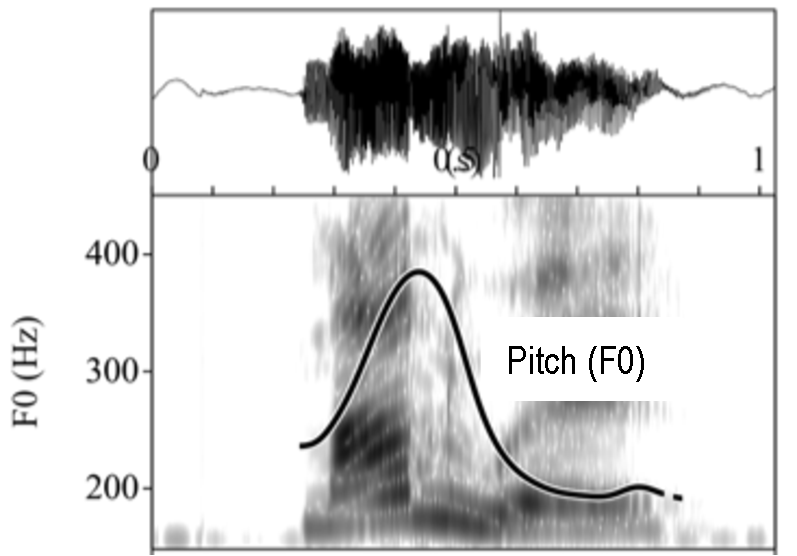
\includegraphics[width=\textwidth]{figures/a02HabilTheory-img003.emf}
%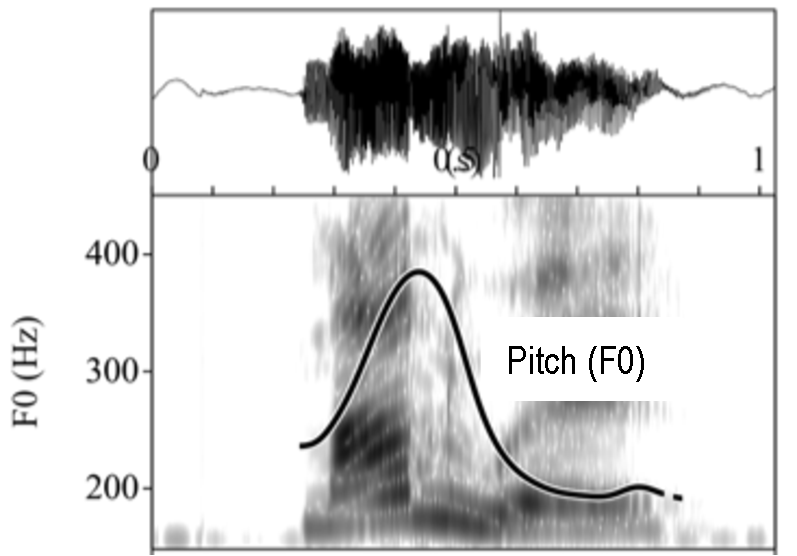
\includegraphics[width=\textwidth]{figures/a02HabilTheory-img003.pdf}
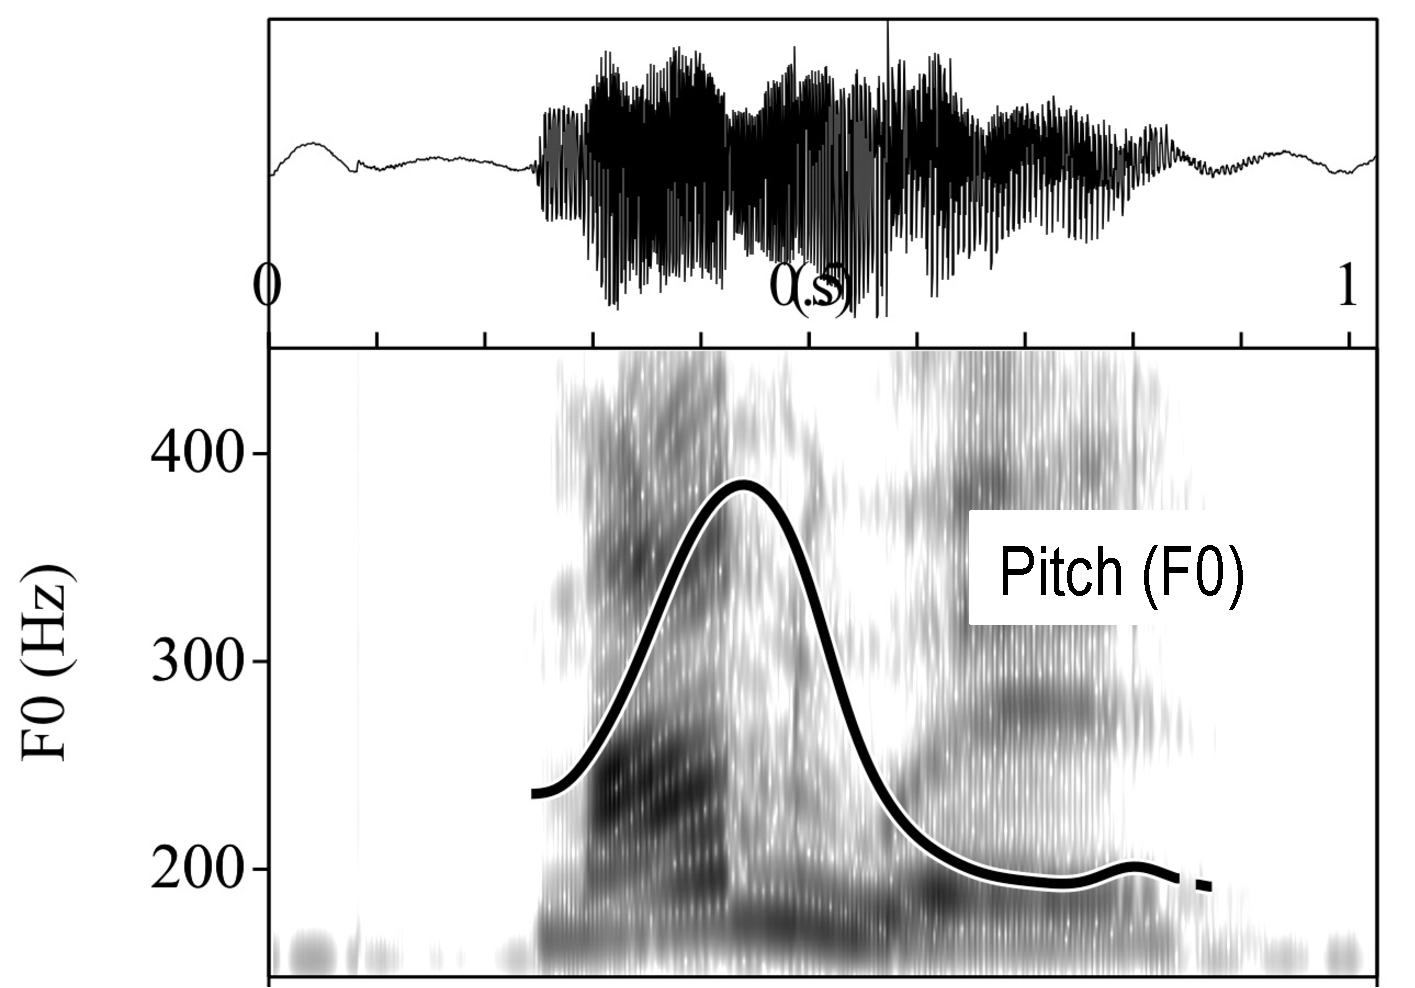
\includegraphics[width=.6\textwidth]{figures/Figure_2.2.pdf}
\caption{Track of the fundamental frequency (F0) in a spectrogram (Praat picture).}
\label{fig:2.2}
\end{figure}

However, not all uses of F0 or pitch are equivalent to intonation; for example, F0 is also used to encode lexical tonal contrasts in some languages (e.g., Mandarin Chinese) or to express paralinguistic information such as boredom or anger (see e.g. \citealt{Arvaniti2022}). More precisely, intonation is defined as the use “of \textit{suprasegmental} phonetic features to convey ‘postlexical’ or \textit{sentence-level} pragmatic meanings in \textit{a linguistically structured} way” \citep[4]{Ladd2008}. In other words, the modulation of pitch that stretches over entire utterances is not random since intonation has not only different functions but, most importantly, its own grammar within a linguistic system (e.g., \citealt{Bolinger1957, Pierrehumbert1980}). \textit{Postlexical} means that it is not determined in the lexicon, in opposite to tone (in tonal languages), stress and quantity (\citealt{HirstDiCristo1998}). Besides the grammatical or discourse and paralinguistic functions, intonation has also extralinguistic functions since it conveys information about speaker’s age, sex and further characteristics (see, e.g., \citealt[47]{Chun2002}). Furthermore, intonation is an important part of speech organisation, language’s \textit{prosody}, described as “an umbrella term that encompasses interacting phenomena that include rhythmic structure, prominence and prosodic phrasing” \citep[25]{Arvaniti2022}. I will come to the prosodic hierarchy later.


Over the last century, there have been various attempts to describe the melodic patterns of utterances in different languages and a large number of theoretical approaches to their analysis have been proposed (see, e.g., \citealt{PassyRambaud1897}, \citealt{Delattre1966} for French; \citealt{Klinghardt1923} for German;  \citealt{NavarroTomás1948}, \citealt{Quilis1975} for Spanish; \citealt{Pike1945}, \citealt{Bolinger1951,Bolinger1972a} for English; \citealt{Petřík1935a, Petřík1935b}, \citealt{Mathesius1937}, and \citealt{Daneš1957,Daneš1985} for Czech; see also \citealt{Prieto2003, Ladd2008,Ladd2015, Elvira-GarcíaEtAl2016, GiliFivelaEtAl2015, NiebuhrWard2018} for overviews on different previous and current models). However, interest in intonational research has increased very rapidly especially in the last four decades by reason of theoretical proposals on the one hand, and information technology development, on the other. Since the acoustic characteristics of intonational contours can be described and measured by means of different language technologies, “they can also be transcribed” (\citealt[768]{Elvira-GarcíaEtAl2016}). Today, there are several different systems for transcription or annotations and models of intonation (within different frameworks) available, including the IPO model (\citealt{HartEtAl1990}), the Tilt Model \citep{Taylor2000}, INTSINT \citep{HirstEtAl2000}, IViE \citep{Grabe2001}, PENTA \citep{Xu2005}, \textit{Rapid Prosody Transcription} (\citealt{ColeShattuck-Hufnagel2016}), and DIMA \citep{KüglerEtAl2015} among others. Nevertheless, one of the most popular systems for annotating intonation is ToBI, \textit{\textbf{To}nes and \textbf{B}reak \textbf{I}ndices} \citep[155]{Hualde2003}, which will also be applied in the present study (presented below). This system for the prosodic annotation of speech was introduced in 1992 for Mainstream American English (\citealt{SilvermanEtAl1992, BeckmanHirschberg1994, BeckmanEtAl2005}), but its original conventions have since been accepted and modified not only for several further English varieties but also for a large number of different languages (see, e.g., \citealt{Jun2005,Jun2014} for an overview of different ToBI systems; \citealt{BeckmanEtAl2005} for the evolution of the ToBI framework). It is important to note that ToBI is grounded in the Autosegmental-Metrical model (AM) of intonational phonology (\citealt{Pierrehumbert1980, Ladd1996}). The AM model is, as \citet[52]{Arvaniti2022} emphasizes, “fundamentally a phonological system and as such relies on the combined investigation of form and meaning” and in order to understand it, it is necessary to understand the general “organization of sound systems which recognizes both the need of abstraction and the need for phonetic detail” (see also \citealt{Arvaniti2019} for cross-linguistic variation, phonetic variability, and the formation of categories in intonation). The AM model has its roots in the British School and in studies on metrical structures and autosegments (e.g., \citealt{OConnorArnold1961, Bolinger1957, Liberman1975, Goldsmith1976, Selkirk1980}). It is called \textit{autosegmental} because the tones (T) representing the melodic part of an utterance are independent from the segments (vowels and consonants) and \textit{metrical} because they are contained in a hierarchically organised set of phonological constituents representing prominence and phrasing. These two sub-systems of (the non-linear) phonology are essential for intonation. The AM theory assumes that speech is organised in abstract, hierarchically levelled constituents, where each constituent of a lower level is enclosed within higher-level constituents. This Prosodic Hierarchy (see \citealt{Selkirk1984, NesporVogel1986/2007, Gussenhoven2002,Gussenhoven2004}, and others) with a commonly adopted set of prosodic constituents and the association of tonal events according to the AM model is depicted in \figref{fig:2.3}.




\begin{figure}
%%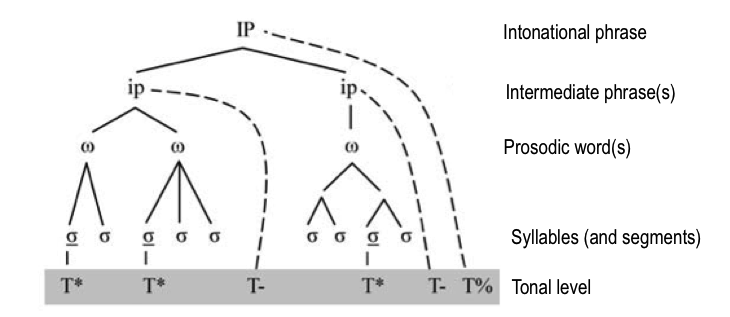
\includegraphics[width=\textwidth]{figures/a02HabilTheory-img004.png}
\begin{forest}
[IP, name = iptop, s sep=8mm
  [ip, name = ipl
    [$\omega$
      [\ul{$\sigma$}, tier=syl
        [T*, tier = word]
      ]
      [$\sigma$, tier=syl]
    ]
    [$\omega$
      [\ul{$\sigma$}, tier=syl
        [T*, tier = word, name = Tl]
      ]
      [$\sigma$, tier=syl]
      [$\sigma$, tier=syl]
    ]
  ]
  [ip, name = ipr
    [$\omega$, name=omega
      [
      [$\sigma$, tier=syl]
      [$\sigma$, tier=syl]
      ]
      [
      [\ul{$\sigma$}, tier=syl
        [T*, tier = word, name = Tr]
      ]
      [$\sigma$, name = sigma, tier=syl]
      ]
    ]
  ]
]
\node[right = 1.3cm of Tl] (T-l) {T-};
\node[right = 7mm of Tr] (T-r) {T-};
\node[right = 3mm of T-r] (T0) {T\%};
\draw[dashed] (ipl) to[out=east,in=north]  (T-l);
\draw[dashed] (ipr) to[out=east,in=north]  (T-r);
\draw[dashed] (iptop) to[out=east,in=north,looseness=1.75]  (T0);
\node[right = 2mm of T0, font=\small] {Tonal level};
\node[right = 1.9cm of sigma, font=\small, align=left] {Syllables\\(and segments)};
\node[right = 3cm of omega, font=\small] {Prosodic word(s)};
\node[right = 3cm of ipr, font=\small] {Intermediate phrase(s)};
\node[right = 5cm of iptop, font=\small] {Intonational phrase};
\end{forest}


\caption{Prosodic Hierarchy based on AM theory (adapted from \citealt[102]{GabrielEtAl2013b}).}
\label{fig:2.3}
\end{figure}

Regarding the tonal level, there are two main elements connected to different layers of the Prosodic Hierarchy: (1) tones or pitch accents which are associated with tonic syllables and marked by a star (T*), and (2) tones which signal lower, hierarchically minor or intermediate (ip) prosodic boundaries (T-) and tones which signal higher, hierarchically major or intonational (IP) prosodic boundaries (T\%).


According to \citet{Ladd1996, Ladd2008}, languages differ intonationally along the following four dimensions: (1) the \textit{semantic dimension}: languages differ in the meaning or use of the same tune (e.g., a low boundary tone can be used for a yes/no question in one language (or dialect) but not necessarily in another); (2) the \textit{systemic} \textit{dimension}: languages differ in the inventory of phonologically distinct tune types (e.g., Catalan has more contrastive tunes than Friulian, where we find more “ambiguous” tunes, see \citealt{RoseanoEtAl2015}); (3) the \textit{realisational dimension}: languages differ in the phonetic implementation of the structural elements (e.g., a rising tone in prenuclear position can be aligned with the tonic syllable in one language, whereas with the posttonic syllable in another); and (4) the \textit{phonotactic} or \textit{distributional} \textit{dimension}: languages differ in tune–text association (e.g., certain tune sequences can be associated either with the beginning or with the end of the text; \citealt[116--118]{Ladd2008}). These dimensions are crucial for the L2 Intonation Learning theory \citep{Mennen2015}, which will be presented later (see \sectref{sec:2.4.2}).


\subsection{ToBI: System for annotating intonation}\label{sec:2.2.2} %2.2.2 /

The main assumptions from the AM model outlined briefly above are also essential for understanding how the ToBI annotation system works. ToBI is an AM tool, which offers a \textit{featural} transcription in the sense that certain symbols represent basic tonal features. Some essential characteristics of the AM model will be explained here. As noted above, the transcription (or annotation) of the pitch track (F0) is based on two important tonal entities: (1) \textit{pitch accents} (PA) or tonal movements associated with the metrically strong (tonic) syllables (the stressed syllable is an important tone-bearing unit (TBU)); and (2) \textit{boundary tones} (BT) or tonal movements related to the edge of an intermediate or intonational prosodic phrase. Therefore, the name ToBI is derived from \textit{tones}, referring to pitch accents, and \textit{break}{}-\textit{indices}, indicating prosodic grouping of the words in an utterance \citep{PriceEtAl1991}. Break indices (BI) receive a number (0--4) referring to how strong the break between words or phrases is. Following general ToBI conventions, a level 0 (or BI 0) marks cohesion between orthographic words (e.g., between a phonologically dependent clitic and a lexical word, its host) that make up one prosodic word, which bears only one pitch accent (e.g., Sp. \textit{la casa} ‘the house’). BI 1 designates boundaries between two prosodic words (e.g., Sp. \textit{la casa grande} ‘the big house’). BI 2 is mostly reserved for non-phonological breaks such as hesitations.\footnote{In the case of phrase languages like French and Czech, there is a BI 2 (phonological) boundary at the edge of the accentual phrases (AP) (see \sectref{sec:2.3.2}).} In contrast to other languages like French \citep{Delais-RoussarieEtAl2015}, there is no consensus among researchers regarding level 2 in Spanish or Italian (see, e.g., \citealt{HualdePrieto2015} for Spanish;  \citealt{GiliFivelaEtAl2015} for Italian). It merely reflects a perceived disjuncture with no intonational effect, and no slowing or other break cues. A level 3 is assigned at the edge of the Intermediate Phrase (ip), which is dominated by the BI 4, the Intonational Phrase (IP) corresponding to the end of main prosodic units (see \citealt{FrotaEtAl2007} for prosodic phrasing in different Romance languages).


These specified tonal targets (PA and BT) are the most important units, where\-as the rest of the contour is formed by phonetic interpolation between them, which is not phonological. The last pitch accent before any ip or IP boundary is called a nuclear accent, whereas the preceding pitch accents are counted as prenuclear pitch accents. ToBI operates with two basic tone levels and their possible combinations, a high tone (H) versus a low tone (L) in the local pitch range. The high targets are not obligatorily aligned with the tonic syllables; the tonal peak of the pitch accent can be reached, for instance, at the end of the posttonic syllable. For such cases, ToBI uses further diacritics for additional information. The alignment for the late peak is tagged with the symbol ``<'' (this is used when the H tone is aligned with the posttonic syllable). Furthermore, ToBI uses the tags ``!'' for downstep (when the pitch of a tonal unit is lower than the pitch of the preceding tone) and ``¡'' for upstep (when the pitch of a tonal unit is higher than the pitch of a preceding tone or its pitch range is wider). We usually do not transcribe a \textit{downstep} (!H) when it is predictable, for example, by the declination in statements, but we always do transcribe an \textit{upstep} (¡H). The diacritics are used for refining phonetic differences between tonal units, or, phonologically, when two entities stand in contrast, that is, when speakers associate the tones with two different meanings. Further details on labelling applied in this study will be presented in \chapref{ch:3}.



Although ToBI is designed to be language-specific and several ToBI annotation systems for different languages have already been proposed (e.g., GToBI for German, Sp\_ToBI for Spanish, Cat\_ToBI for Catalan, K-ToBI for Korean), there is also a set of community-wide conventions adopted by all ToBI users. First of all, the analysis of phonetic evidence must be based on both auditory perception and visual examination of the F0 curve by means of a specific program for phonetic analysis of speech (e.g., Praat). Next, it is univocal: for example, a high tone is always transcribed as H(igh) and H cannot be used for another entity. ToBI labellers thus agree to adopt the same labels and to maintain consistency (which does not mean that changes are prohibited). And finally, it is “easy to teach” and “accessible to a fairly wide audience, without assuming any background in linguistics or speech sciences” (see English ToBI at \url{https://www.ling.ohio-state.edu/~tobi/} and Spanish ToBI at \url{http://prosodia.upf.edu/sp\_ tobi/en/index.php}). While it is true that ToBI is easy to learn and understand, its simplicity and practical application to data are not unproblematic and ToBI annotation implies several important requirements. Initially, a labeller must have \textit{a priori} knowledge of the language under study and above all its phonology, must be familiar with (acoustic) phonetics, and must possess advanced user skills for Praat (or any other similar program), in order to avoid software errors and prevent micro-prosody effects from shaping the pitch contour. In addition, the labeller must be able not only to read the shape of F0 contours but also to understand how prosody functions to mark grammatical contrasts in that language (see, e.g., \citealt{Arvaniti2016}) because tonal targets have a linguistic meaning and important function in phonological, morphological, semantic, pragmatic, and even sociolinguistic contexts (\citealt{JunFletcher2014}). The perception factor should not be underestimated either; some researchers even suggest a “Label what you hear” guideline \citep[28]{Wightman2002}, which should take precedence over the description of the shape of the pitch track (for a similar view see \citealt{Romportl2008}). Notwithstanding, practice has shown that even trained and experienced labellers may still diverge in the way they interpret and transcribe intonational curves. Prosodic annotation is thus challenging for a number of factors, among which \citet{ColeShattuck-Hufnagel2016} list speech rate, style, nuances of pragmatic meanings, reduced or ambiguous acoustic cues as well as influence from the linguistic context. One of the principal difficulties is the potential for differing and subjective interpretations of the phonetic-phonology interface, presupposing the existence of discrete entities (i.e., tones). ToBI is primarily phonological because it shares basic assumptions from AM, which relies on an abstract phonological representation connected with pitch contours, considering intonation an important part of a language’s grammar. However, we often find inconsistencies and phonetic-like instead of phonemic transcription in the studies applying ToBI. Typical sources of confusion for labellers in tagging processes are the transcription of truncated pitch contours, reductions in the acoustic signal, tonal clashes, contrasts of alignment, indications of downstep/upstep, and many other phenomena (\citealt{ColeShattuck-Hufnagel2016, JunEtAl2015, HualdePrieto2016}). Therefore, the introduction of two levels of representation in a prosodic annotation can be a very good solution here: “One, phonological, where meaningless (and predictable) variation in alignment and range is ignored and another, broad phonetic, where these differences are represented” (\citealt[15]{HualdePrieto2016}). According to \citet{HualdePrieto2016}, this can make it easier to understand tonal contrasts in a cross-linguistic perspective but most importantly within one language (for a critical view on broad phonetic transcription, see \citealt{Arvaniti2016,Arvaniti2022, CangemiGrice2016, ColeShattuck-Hufnagel2016}). For example, vocative chants in Catalan have one phonological underlying tone /L+H* !H\%/ with two possible phonetic realizations: [L+H* !H\%] and [H* !H\%] depending on the context (\citealt[13--14]{HualdePrieto2016}). The [L+H* !H\%] variant is phonetically realized as a rise and the [H* !H\%] as a high plateau (H) during the tonic syllable. Both nuclear accents are followed by a sustained mid level plateau (!H). The two allotones are in complementary distribution: If the word begins with an unaccented syllable (e.g., \textit{Ma}\textbf{\textit{ri}}\textit{na!}), the low tone (L) is phonetically realized on the surface (L+H*). On the other hand, if the word begins with an accented syllable and a voiceless plosive (\textbf{\textit{Pau}}\textit{la!}), the L tone is not expressed overtly (H*) (\figref{fig:2.4}).




\begin{figure}
%%\includegraphics[width=\textwidth]{figures/a02HabilTheory-img005.tif}
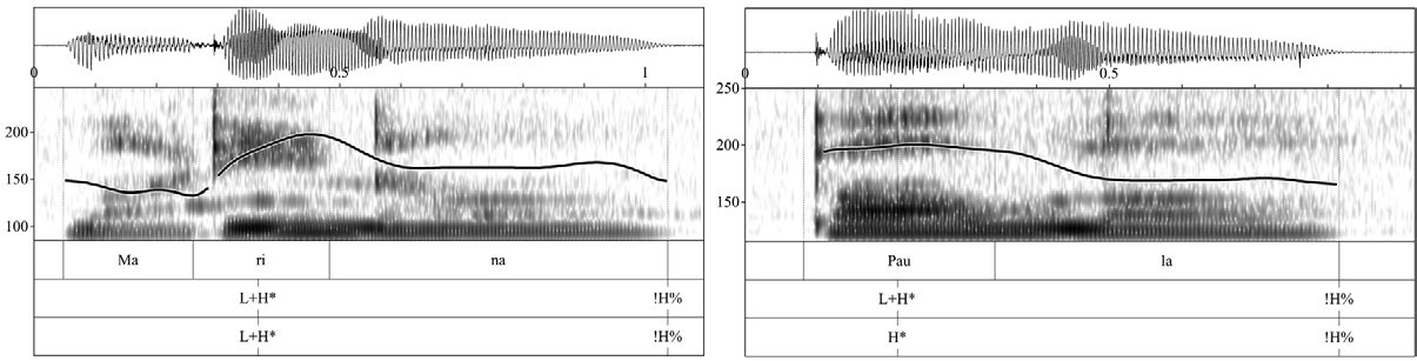
\includegraphics[width=\textwidth]{figures/a02HabilTheory-img005-new.png}


\caption{Phonological (second tier) and broad phonetic (third tier) representations of the vocative chant in Catalan (taken from \citealt[14]{HualdePrieto2016}).}
\label{fig:2.4}
\end{figure}


The treatment of the phonetic-phonology interface, presenting also a notorious degree of variability across speakers and contexts, is still a widely debated and challenging issue in intonational research (see, e.g., \citealt{Wightman2002, BreenEtAl2012, ColeEtAl2014, ColeShattuck-Hufnagel2016, Pešková2018}).



In sum, the ToBI approach has received many criticisms: it is said to be too phonetic, it is too phonological, it is too subjective, it is not applicable to all languages, etc. In my opinion, in spite of these various (and important) critical points, ToBI can be seen as a useful approach for the description and systematization of intonation patterns and “as a tool for testing and evaluating hypotheses to improve the intonation model” (\citealt[518]{JunFletcher2014}). Moreover, several studies have shown by means of intertranscriber reliability tests a high degree of agreement or consistency among trained labellers thus proving the functional utility of ToBI for prosodic annotation (see, e.g., \citealt{PitrelliEtAl1994, YoonEtAl2004, EscuderoEtAl2012, MennenEtAl2012, Feldhausen2016, Elvira-GarcíaEtAl2016}).


\subsection{Application of ToBI labels on L2 data of the present study}\label{sec:2.2.3} %2.2.3 /
\begin{sloppypar}
As the present study deals with L2 intonation contours, here the question emerges: ToBI, or not ToBI? I have decided for a ToBI non-language-specific and phonetic-based labelling in order to provide simplified representations of tonal events, on the one hand, and to systematize and compare the patterns found in data, on the other hand. The aim of the phonetically transparent analysis here is to detect and compare differences between the L1 and L2 systems and to explain non-native productions. The idea of non-language-specific labels is not new and ToBI or AM-based labels for L2 intonation (with modifications or deviations) have already been used in different studies on L2 intonation (e.g., \citealt{JunOh2000, MennenEtAl2012, Mennen2015, AstrucVanrell2016, ColantoniEtAl2016a}, and many others). This annotation with phonetic labels is indirectly in line with the recent -- but so far not overall accepted -- proposal for the development of the \textit{International Prosodic Alphabet} (IPrA) that offers “a set of cross-linguistically transparent and consistent labels” based on ToBI annotation (\citealt[1]{HualdePrieto2016}). According to the authors of this proposal, “the IPrA tool can be useful for L2 prosodic studies […], as right now it is difficult to transcribe L2 speech when working with two established ToBI systems” (\citealt[19]{HualdePrieto2016}, see also \citealt{JunFletcher2014}). A similar view was taken by the authors of the Eti\_ToBI automatic intonation transcriber for Spanish (\textit{El etiquetador ToBI}, \citealt{Elvira-GarcíaEtAl2016}), who argue that “a standard (non-language related) ToBI method for analysing prosody is possible” since it “provides an objective, transparent and universal transcription based only on acoustic data” (\citealt[785]{Elvira-GarcíaEtAl2016}) (see \sectref{sec:3.4.1}). The present study applies or modifies for its purposes these two projects and available AM transcription systems for the languages under study. The following inventory of nuclear pitch accents and boundary tones (ip/IP) proved to be important for the data of the present study (see Figures \ref{fig:2.5}--\ref{fig:2.6} for a schematic representation of the F0 track and Tables~\ref{tab:2.4a}--\ref{tab:2.4b} for a phonetic description of the tonal events). The tonal inventories of the languages under study are presented in \sectref{sec:2.3.2}. We will see examples of these patterns later in Chapters~\ref{ch:3} and \ref{ch:4}.
\end{sloppypar}


\begin{figure}
%%\includegraphics[width=\textwidth]{figures/a02HabilTheory-img006.emf}
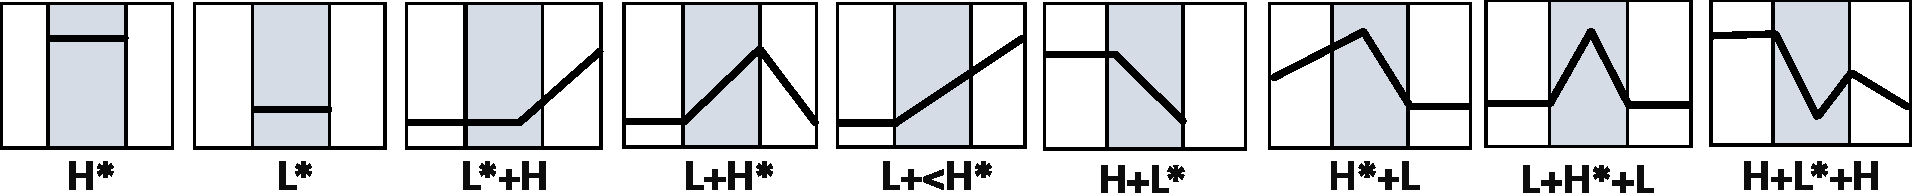
\includegraphics[width=\textwidth]{figures/a02HabilTheory-img006.pdf}
\caption{Schematic representation of pitch accents found in both L1 and L2 data.}
\label{fig:2.5}
\end{figure}

\begin{figure}
%%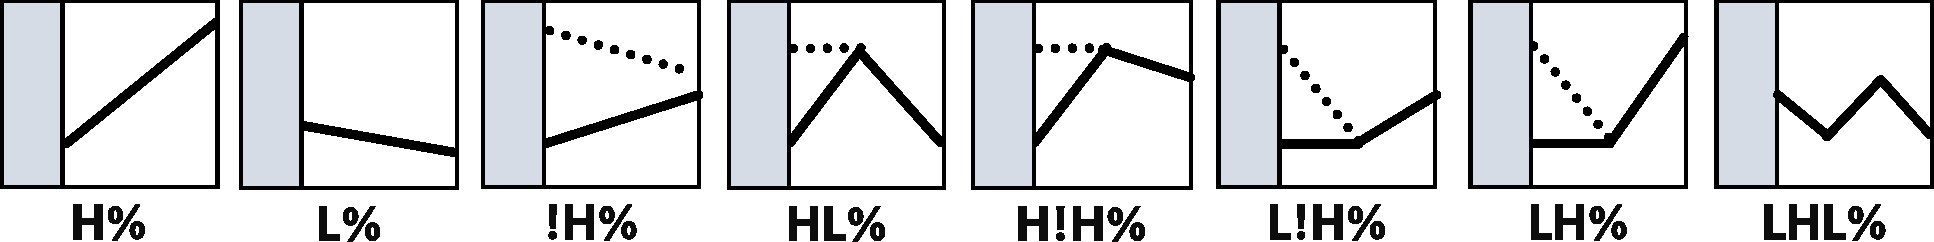
\includegraphics[width=\textwidth]{figures/a02HabilTheory-img007.emf}
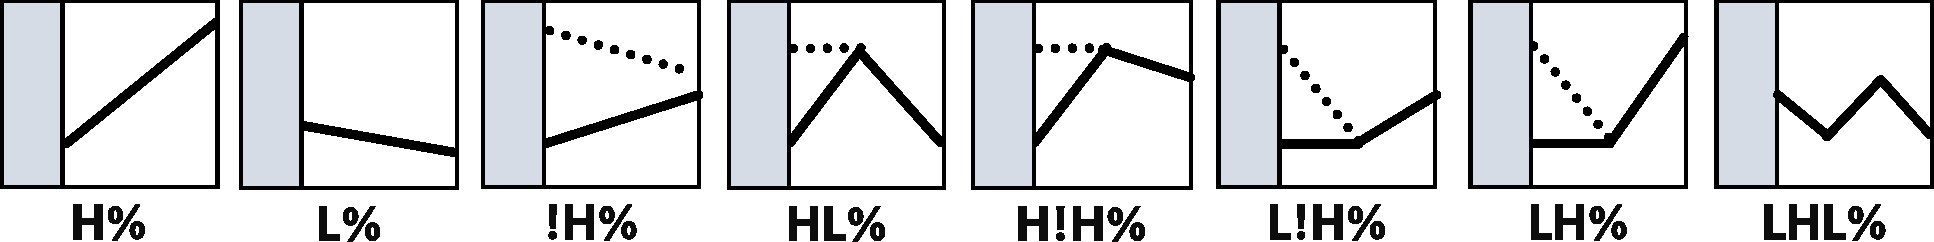
\includegraphics[width=.8\textwidth]{figures/a02HabilTheory-img007.pdf}
\caption{Schematic representation of boundary tones found in the data (the dotted line indicates alternative pitch tracks).}
\label{fig:2.6}
\end{figure}

\begin{table}
\begin{tabularx}{\textwidth}{p{3cm}Q}
\lsptoprule
Tonal entity & Description of the phonetic realization\\\midrule
H* & High plateau without any preceding F0 valley.\\
\tablevspace
L* & Low plateau at the low level of the speaker’s range.\\
\tablevspace
L*+H & Low plateau in the tonic syllable, which is followed by a rising F0 movement in the posttonic syllable.\\
\tablevspace
L+H* & Rising F0 movement during the tonic syllable with the F0 peak located at its end.\\
\tablevspace
L+<H* & Rising F0 movement during the tonic syllable with its F0 peak aligned with the posttonic syllable.\\
\tablevspace
H+L* & F0 fall within the temporal limits of the tonic syllable (with a high target in the pretonic syllable).\\
\tablevspace
H*+L & F0 rising pattern at the beginning and a falling pattern in the tonic syllable. The fall is dominant. \\
\tablevspace
L+H*+L

(L+H* or H*+L in Italian ToBI) & Balanced rising-falling pattern located within the tonic syllable.\\
\tablevspace
H+L*+H

(L*+>H in Italian ToBI) & Falling-rising pattern within the tonic syllable. The start of the fall is (roughly) aligned with the beginning of the tonic syllable. The rise is always smaller than the fall; both occur in the tonic syllable.\\
\lspbottomrule
\end{tabularx}
\caption{Inventory and description of prenuclear and nuclear pitch accents used in the present study. The phonetic description of these tonal representations is based on \citet{AguilarEtAl2009}, \citet{Estebas-VilaplanaPrieto2008}, \citet{GabrielEtAl2010} and  \citet{GiliFivelaEtAl2015}.\label{tab:2.4a}}
\end{table}


\begin{table}
\caption{Inventory and description of boundary tones (ip, IP) used in the present study. The phonetic description of these tonal representations is based on \citet{AguilarEtAl2009}, \citet{Estebas-VilaplanaPrieto2008}, \citet{GabrielEtAl2010} and  \citet{GiliFivelaEtAl2015}.\label{tab:2.4b}}
\begin{tabularx}{\textwidth}{lQ}
\lsptoprule
{Tonal entity} & {Description of the phonetic realization}\\
\midrule
H-, H\% & Rising F0 movement after a H or L pitch accent.\\
\tablevspace
L-, L\% & Low sustained or falling tone at the speaker’s baseline.\\
\tablevspace
!H-, !H\% & Slightly rising or falling F0 movement towards a middle target (also called “sustained” pitch).\\
\tablevspace
HL-, HL\% & F0 peak with a subsequent fall.\\
\tablevspace
H!H-, H!H\% & F0 peak with a slight fall towards a middle target.\\
\tablevspace
L!H-, L!H\% & Low sustained tone followed by a slightly rising F0 movement towards a middle target.\\
\tablevspace
LH-, LH\% & Low sustained tone followed by a sharp rising F0 movement.\\
\tablevspace
LHL-, LHL\% & Complex pitch movement consisting of a fall plus rise and then a fall to a low F0 value. (This pattern is attested only in L1 Spanish in exhortative requests.)\\
\tablevspace
Hi & Initial pitch (sometimes transcribed as \%H). This high tone marks a phrase at the beginning of the speaker’s pitch range and is not attributed to the first pitch accent of the utterance. It was transcribed only if it was articulated as a high plateau which could not be attributed to a high pitch accent (H*); this was the case when the first word of an utterance begins with an unaccented syllable. \\
\lspbottomrule
\end{tabularx}
\end{table}


In general, there are no major differences between the labels used here and those applied in previous work. However, the present study differs with regard to the treatment of tritonal pitch accents. In comparison to the IPrA and the ToBI systems, which usually do not account for tritonal realizations of pitch accents, the present work includes two tritonal pitch accents (H+L*+H, L+H*+L) in its analysis. The H+L*+H tone reported here is similar to an IPrA H+!H* tone, but they are not identical: H+L*+H has a sharp fall and a moderate rise to a mid level, whereas a H+!H* has a falling pattern to a mid level.\footnote{The H+!H* tone has been documented, for example, in German \citep{GriceEtAl2005a} and French \citep{Delais-RoussarieEtAl2015}. It is very similar to H+L*, a label which is used here.}  It corresponds to the Italian L*+>H in  \citet{GiliFivelaEtAl2015}, but the label H+L*+H is preferred here in order to specify the exact tritonal F0 movement within the stressed syllable. As for L+H*+L, it has an equilibrated rising-falling pattern located within the tonic syllable (mostly the tonic vowel) and it is thus realized and perceived differently from H*+L, H+L* or L+H*. The tag L+H*+L has been proposed for Pisa Italian (\citealt{GiliFivela2002,GiliFivela2004, PrietoEtAl2005}) as well as Argentinean Spanish (an “Italianized” variety of Spanish, see, e.g., \citealt{GabrielEtAl2010, GabrielKireva2014a}). Production and perception experiments motivated the assumption that L+H*+L is the phonological nuclear accent for expressing focus, contrast or emphasis in Argentinean Spanish (see, e.g., \citealt{GabrielEtAl2010, FeldhausenEtAl2011}). In Italian, a tritonal pattern as an underlying category has not been fully accepted:  \citet[148]{GiliFivelaEtAl2015} point out that the pattern with a tritonal shape within the stressed syllable belongs to the underlying ``early-peak'' (L+H*) pattern or H*+L depending from L1 Italian varieties (see, for instance, nuclear pitch accents in their examples in Fig. 5.5, pg. 162; see also  \citealt{GiliFivela2002,GiliFivela2004} for further details).\footnote{L+H*+L is regarded as a phonetic variant of the phonological pattern /H*+L/ by \citet{GiliFivela2002, GiliFivela2004}, who leaves the leading tone [L] merely for phonetic purposes because the trailing pattern is sufficient for phonological contrast.}


The following section presents phonological systems of the languages under study, including their segmental and suprasegmental features.


\section{Phonological systems of the languages under study}\label{sec:2.3}

The objective of this section is to present and compare the main segmental and suprasegmental properties of the languages under study. Since foreign accent is a typical feature of L2 speech and articulation of segments plays an important role in it, first, segmental dissimilarities and similarities across the languages under study are considered (\sectref{sec:2.3.1}). Next, the main suprasegmental characteristics, including rhythm, stress and intonation, together with the prosodic typology of the languages are presented (\sectref{sec:2.3.2}).

\subsection{Segmental inventories in contrast}\label{sec:2.3.1} %2.3.1 /

The comparison of the systems predicts where the learners might have major problems with target-like pronunciation and according to which -- potentially transferred -- vowels and consonants we might be able to distinguish a German L2 learner from a Czech L2 learner. Given the fact that segments are not the main focus of this study, I will present only the most important phenomena, without going into a detailed discussion on dialectal differences or factors such as speaking style. The summary in \tabref{tab:2.5a} is based on the following literature: \citet{Canepari1992}, \citet{RogersdArcangeli2004}, \citet{LoporcaroBertinetto2005} for Italian; \citet{Hualde2005, Hualde2014}, \citet{GabrielEtAl2013a} for Spanish; \citet{Palková1994}, \citet{Dankovičová1999}, \citet{Volín2010}, \citet{ŠimáckováEtAl2012}, \citet{SkarnitzlEtAl2016} for Czech; \citet{Kohler1995, Kohler1990, Kohler1999}, \citet{Mangold2005}, \citet{Hall2011}, \citet{MeibauerEtAl2015} for German. Some transferred phenomena will be illustrated by means of the L2 data collected in the production experiment of the present study (see \chapref{ch:3}).

\begin{sidewaystable}

\begin{tabularx}{\textwidth}{QQQQQ}

\lsptoprule

{Segmental} & \multicolumn{2}{l}{{Target languages}} & \multicolumn{2}{l}{{L1 backgrounds}}\\
\cmidrule(lr){2-3}\cmidrule(lr){4-5}
Features & {Italian} & {Spanish} & {Czech} & {German}\\
\midrule
Vowel quality & / a e ɛ i o ɔ u / & / a e i o u / & / a ɛ ɪ o u

aː ɛː iː oː uː / & / i y ɪ ʏ e ø ɛ œ ə ɐ a ɑ ɔ o ʊ u / \\
\tablevspace
Vowel quantity & No phonemic opposition

(but stressed open vowels are longer) & No phonemic opposition & Phonemic opposition & Phonemic opposition only in stressed syllables\\
\tablevspace
Vowel reduction & No & No & No & Yes \\
\tablevspace
Consonant quantity & Geminates & No geminates & No geminates & No geminates\\
\tablevspace
VOT / p t k / & Zero VOT & Zero VOT & Zero VOT & Positive VOT

(aspiration)\\
\tablevspace
VOT / b d ɡ / & Negative VOT & Negative VOT & Negative VOT & Zero VOT\footnote{For a better comparison, I use the term ``zero VOT'' (e.g., \citealt{RakowLleó2008}), although voiceless plosives show a certain degree of positive VOT and ``devoicing'' \citep[58]{Catford1988} might be an alternative term here.}\\
\tablevspace
Pronunciation of

/ b d ɡ / & Plosive & Plosive or Approximant

[β ð ɣ] & Plosive & Plosive\\
\midrule
\end{tabularx}
\caption{Main segmental features of Italian, Spanish, Czech and German in contrast.}
\label{tab:2.5a}
\end{sidewaystable}
\begin{sidewaystable}\ContinuedFloat

\begin{tabularx}{\textwidth}{QQQQQ}

\midrule

{Segmental} & \multicolumn{2}{l}{{Target languages}} & \multicolumn{2}{l}{{L1 backgrounds}}\\
\cmidrule(lr){2-3}\cmidrule(lr){4-5}
Features & {Italian} & {Spanish} & {Czech} & {German}\\
\midrule
Final-obstruent devoicing & No & No & Yes & Yes\\
\tablevspace
Pronunciation of rhotics & [r] & [r], [ɾ] & [r] & [ʁ], usually vocalized in coda position\\
\tablevspace
Pronunciation of laterals & “light” /l/ & “light” /l/ & velarized or “dark” /l/ & “light” /l/\\
\tablevspace
Further potential difficulties for L2 learners & [ʎ] & [ʎ], [θ], [ʝ] & -- & --\\
\tablevspace
Syllable structure\footnote{See WALS \citep{Maddieson2013} for the terms used here.} & Moderately complex syllable structure & Moderately complex syllable structure & Complex syllable structure & Complex syllable structure\\
\tablevspace
C\#V sequences & Resyllabification & Resyllabification & Optional resyllabification; optional assertion of glottal stop before initial vowels & No resyllabification; assertion of glottal stop before initial vowels\\
\lspbottomrule
\end{tabularx}


%\caption{Main segmental features of Italian, Spanish, Czech and German in contrast (continued).}
%\label{tab:2.5b}
\end{sidewaystable}

\subsubsection{Vowels}\label{sec:2.3.1.1}

First of all, we observe that the two Romance languages display quite a limited vowel system. Both have no phonemic opposition in duration, although traditionally it has been claimed that in Italian vowels in stressed open syllables have longer duration than unstressed vowels or vowels in closed syllables. Against this traditional phonetic approach, however, \citet{DImperioRosenthall1999} have proved that the increased duration is not equal in all positions and have proposed that the lengthening of penultimate syllables is phonological. In contrast, Czech is a typical quantity language in that it differentiates phonologically between short and long vowels, the durational ratio between them being about 1:1.3--1.8 depending on the vowel (\citealt[51]{SkarnitzlEtAl2016}). The durational opposition is allowed in both stressed and unstressed positions in Czech (e.g., [ˈmɪ.laː], ‘kind-\textsc{f}’ vs. [ˈmɪ.la] ‘she washed’). In this respect, Czech differs substantially from the other languages, in which unstressed vowels cannot be longer than stressed vowels (with the exception of final/preboundary syllables, which are intrinsically longer) (see also \sectref{sec:2.3.2}). This is also why many non-native speakers may perceive unstressed syllables with a long vowel as stressed syllables in Czech (e.g., \textit{Janáček} [ˈjanaːtʃɛk], perceived as [jaˈnaːtʃɛk]). Notice that a long vowel is orthographically marked with an acute accent in Czech. Due to the similarities in vowel quality, Czech learners have no special difficulties with the acquisition of the Italian or Spanish vowel systems. The only problem that can arise is with the opposition of /e/ vs. /ɛ/ and /o/ vs. /ɔ/ in Italian. German has the most complex vowel quality system, displaying also durational opposition, which is restricted to stressed syllables. Additionally, it reduces or deletes vowels in unstressed positions; this property is very often transferred to an L2. For example, the unstressed vowel /o/ in the Spanish word \textit{perro} ‘dog’ is usually pronounced in a very close-mid manner, what natives might perceive as something like [u].\pagebreak

\subsubsection{Consonants}\label{sec:2.3.1.2}

Regarding the pronunciation of consonants, every language shows its own particularities. Italian is a language that geminates consonants, a property causing difficulties for many L2 learners who do not have this feature in their phonological systems. Spanish is the only language that displays approximant allophones [β ð ɣ] of the voiced plosives in specific contexts, and this is where many L2 learners show articulation difficulties even at a very advanced level. In contrast, German is the only language that -- under certain conditions -- aspirates voiceless stop consonants and has zero VOT in the case of voiced stops, meaning that there is (almost) no voicing at the instant of the articulation closure. This is why native hearers tend to interpret German learners’ [b d ɡ] as [p t k] (e.g., the Spanish word \textit{drama} ‘drama’ may sound like \textit{trama} ‘plot’). \figref{fig:2.7} offers an example of an aspirated /t/ in L2 Spanish as produced by an L1 German learner.\footnote{I applied the figure-drawing Praat script by \citet{Elvira-García2014} to generate all Praat figures in the text.} Notice that the intervocalic /b/ was not produced as an approximant [β] in accordance with the rules of Spanish phonology.


\vfill
\begin{figure}[H]
%%\includegraphics[width=\textwidth]{figures/a02HabilTheory-img008.tif}
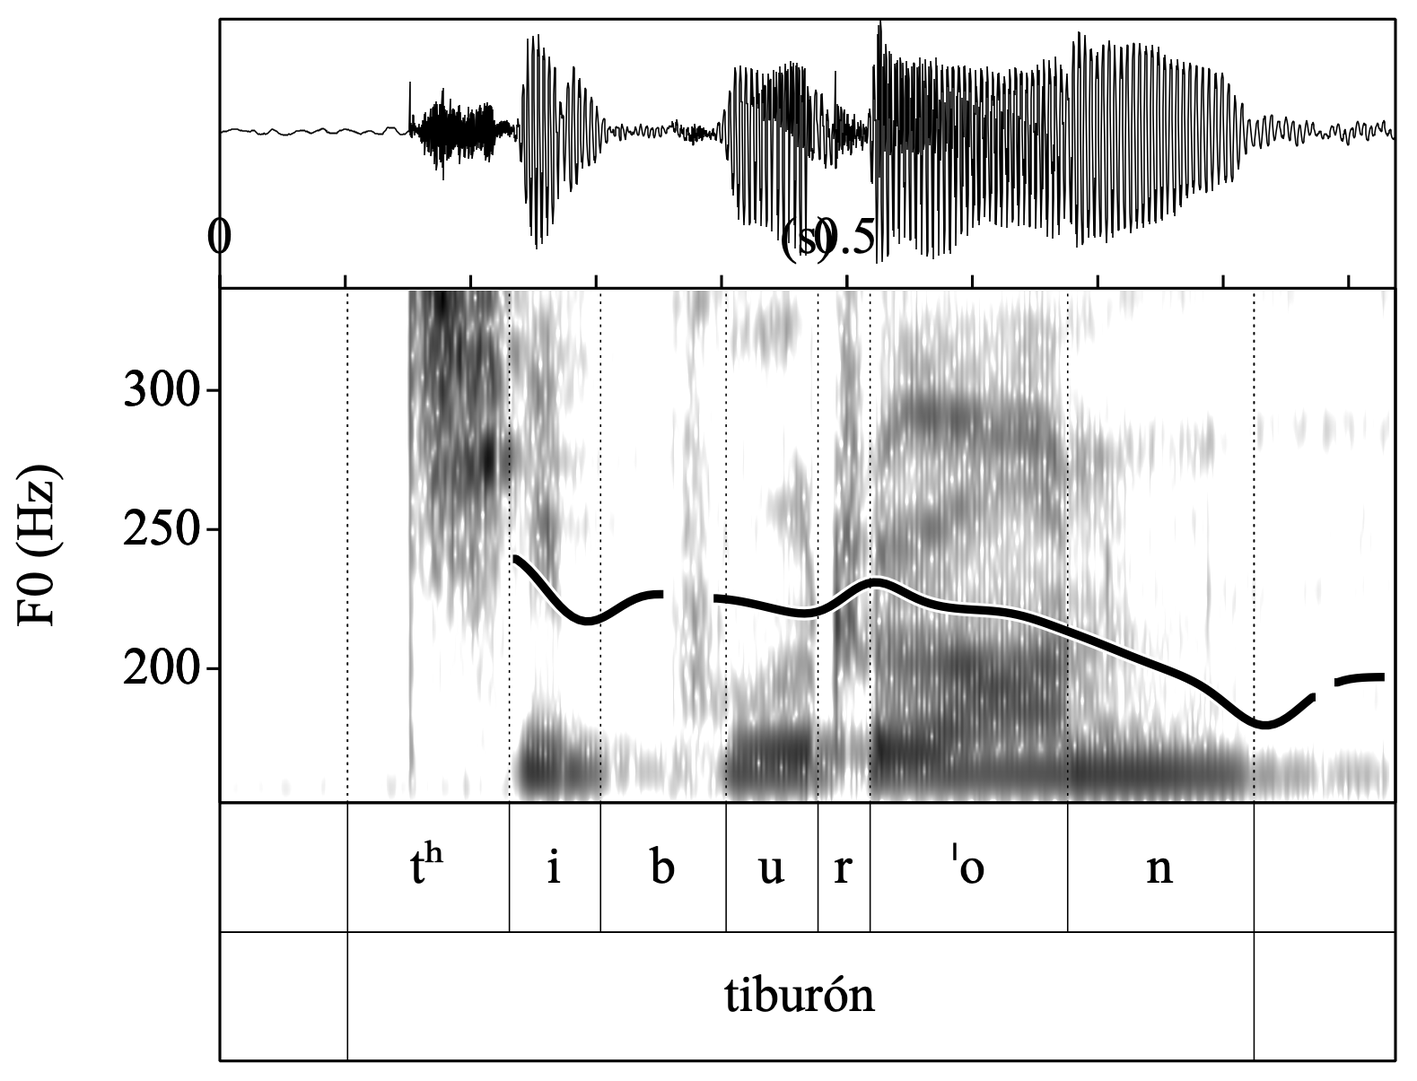
\includegraphics[width=.7\textwidth]{figures/a02HabilTheory-img008-new.png}
\caption{Aspiration of /t/ in the word \textit{tiburón} ‘shark’ in L2 Spanish produced by an L1 German learner (F\_19).}
\label{fig:2.7}
\end{figure}
\vfill\pagebreak


In contrast to Italian and Spanish, German and Czech show final-obstruent devoicing, which can be observed in L2 as well (\figref{fig:2.8}).\footnote{The correct pronunciation of the final consonant in this position in Spanish would be [\textrm{baɾ.βa.ɾi.ˈðað}], [\textrm{baɾ.βa.ɾi.ˈða}\textrm{\textsuperscript{ð}}], [\textrm{baɾ.βa.ɾi.ˈða}] or [\textrm{baɾ.βa.ɾi.ˈðaθ}], depending on the speech style and/or dialect. In Italian, the voiced obstruent is maintained in such cases (e.g., <sud> [\textrm{ˈsud}], ‘south’).}



\begin{figure}
%%\includegraphics[width=\textwidth]{figures/a02HabilTheory-img009.tif}
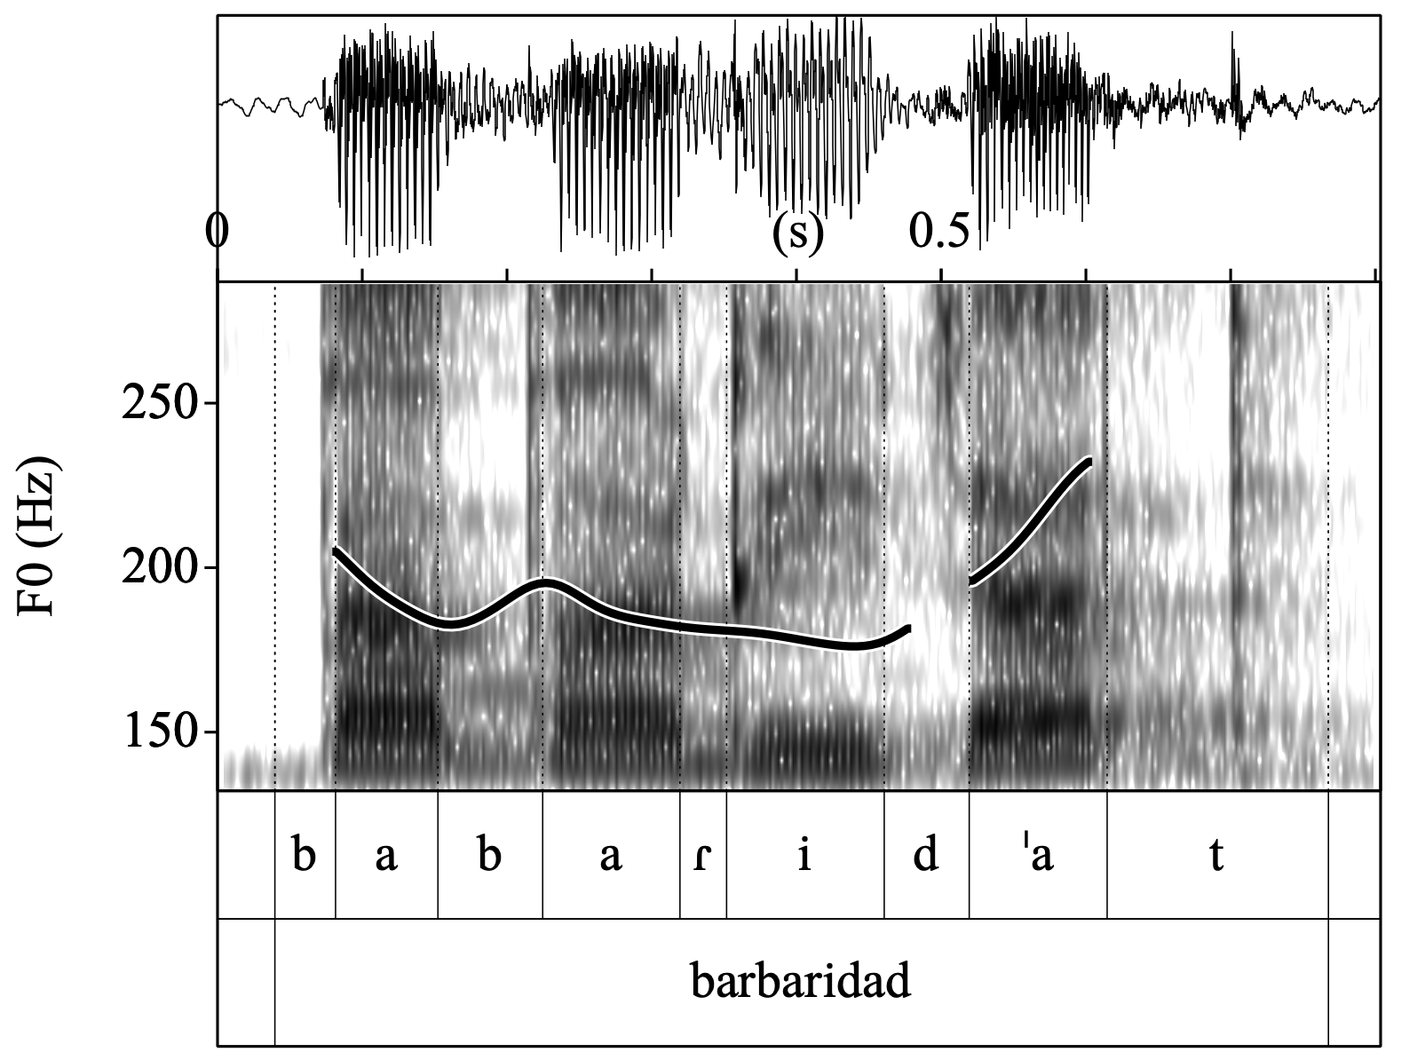
\includegraphics[width=.7\textwidth]{figures/a02HabilTheory-img009-new.png}



\caption{Final-obstruent devoicing of /d/ in the word \textit{barbaridad} (‘barbarity’) in L2 Spanish produced by an L1 German learner (F\_06).}
\label{fig:2.8}
\end{figure}


It is well known that the pronunciation of Spanish rhotics causes the most difficulty for German learners, who do not have this sound in their L1 consonant inventory. Thus, German learners can be easily identified by the mispronunciation of the rhotics (trill and tap), together with the aspiration of voiceless stop consonants, the devoicing of voiced stops and vowel reduction. On the other hand, Czech learners can be recognized, for instance, on the basis of their velarized or “dark” /l/.


Further potential difficulties can be found with the sounds /ʎ θ ʝ/, which are not present in the Czech and German segmental systems. Moreover, some phenomena are connected not with an articulation problem but with the impact of literacy. As already mentioned in \sectref{sec:2.1.7}, the L1 orthography strongly shapes L2 speech, especially at the beginning of the acquisition process. For example, German but also Czech learners of Spanish tend to pronounce <h> as [h] or [ɦ] (this is valid also for Czech learners of Italian), they voice <s> in certain intervocalic positions or pronounce <v> as a labiodental fricative [v], which is absent in the majority of Spanish dialects. Additionally, Czech learners of the Romance languages show a tendency to lengthen vowels with an acute diacritic (e.g., <é>), in accordance with the rules applied in L1 Czech orthography (in Spanish or Italian, the acute indicates lexical stress). An example of the impact of Czech orthography on L2 Spanish is given in \figref{fig:2.9} (more details are provided in \citealt{PeškováEtAl2017}). Here the first <é> in \textit{él vino} (‘he came’) is long and forms 26\% of the whole speech signal (610\,ms), whereas the second <e> in \textit{el vino} (‘the wine’) is short and forms only 16\% of the signal (580\,ms). Notice also that the Czech learner produced the letter <v> not as a target-like [β] but as a [v], in line with Czech orthography.



\begin{figure}
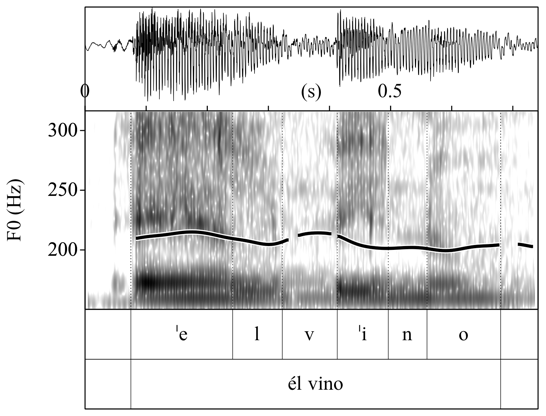
\includegraphics[width=.475\textwidth]{figures/a02HabilTheory-img010.png}\hfill
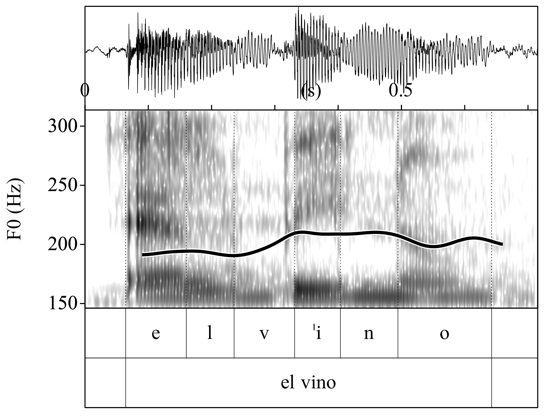
\includegraphics[width=.475\textwidth]{figures/a02HabilTheory-img011.png}
\caption{The pair \textit{él vino} (left) and \textit{el vino} (right) and the influence of orthography on the vowel lengthening in L2 Spanish produced by a L1 Czech learner (F\_07).}
\label{fig:2.9}
\end{figure}


\subsubsection{Syllable structures in contrast}\label{sec:2.3.1.3}

Finally, I will make a brief comment on the combination of segments, that is, on syllable structure. Since German and Czech allow very complex consonant clusters in onsets as well as codas (Czech may even have liquids in the nucleus, e.g., \textit{vlk} ‘wolf’, \textit{prst} ‘finger’), L2 learners have no difficulties with syllable structures in target Spanish and Italian, in which the syllable complexity is much more moderate in terms of the number of possible consonant combinations. Where we might find interferences is in C\#V sequences. In Spanish, the resyllabification rule is systematically applied in connected speech to form “ideal” or prototypical CV syllables (V\textbf{C}\#V → V.\textbf{C}V), as illustrated schematically in \figref{fig:2.10}.



\begin{figure}
%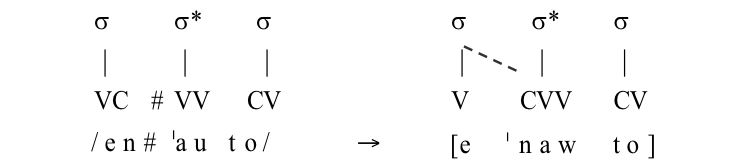
\includegraphics[width=\textwidth]{figures/a02HabilTheory-img012.png}
\begin{forest}
for tree = {align=left,
            baseline=(current bounding box.center)},
[,phantom
  [$\sigma$
    [VC\\/en]
  ]
  [$\sigma$*
    [\#VV\\\#ˈau]
  ]
  [$\sigma$
    [CV\\to/]
  ]
]
\end{forest}
$\to$
\begin{forest}
for tree = {align=left,
            baseline=(current bounding box.center)},
[,phantom
  [$\sigma$, name = s
    [V\\{[e}]
  ]
  [$\sigma$*
    [CVV\\ˈnaw, name = cvv]
  ]
  [$\sigma$
    [CV\\{to]}]
  ]
]
\draw[dashed] (s.south) -- (cvv.north);
\end{forest}
\caption{Example of the CV resyllabification rule that applies in Spanish (\textit{en} \textit{auto} ‘in the car’).}
\label{fig:2.10}
\end{figure}

\begin{sloppypar}
In Italian resyllabification can also occur (\citealt[72]{NesporVogel1986/2007}), whereas German and Czech maintain the word-boundary (\citealt{Szczepaniak2009, ŠimáckováEtAl2012}).\footnote{However, in accordance with phonotactic patterns, resyllabification in Czech is not as strong and prominent as in German. In Moravian Czech, resyllabification is more common than in Bohemian Czech, where the glottal stop is preferred (\citealt[230]{ŠimáckováEtAl2012}).} Such morphological boundaries in vowel-initial words can have different phonetic realizations, comprising mainly glottalization, glottal stop insertion and/or creaky voice (see, e.g., \citealt{ŠimáckováEtAl2012} for Czech; \citealt{Kohler1994,Kohler1995, Pompino-MarschallZygis2010} for German). These strategies can be frequently observed in L2 productions (\figref{fig:2.11}). Spanish and Italian native speakers usually perceive L2 speech without resyllabification and with glottal stops as interrupted and chopped.
\end{sloppypar}



\begin{figure}

%%\includegraphics[width=\textwidth]{figures/a02HabilTheory-img013.tif}
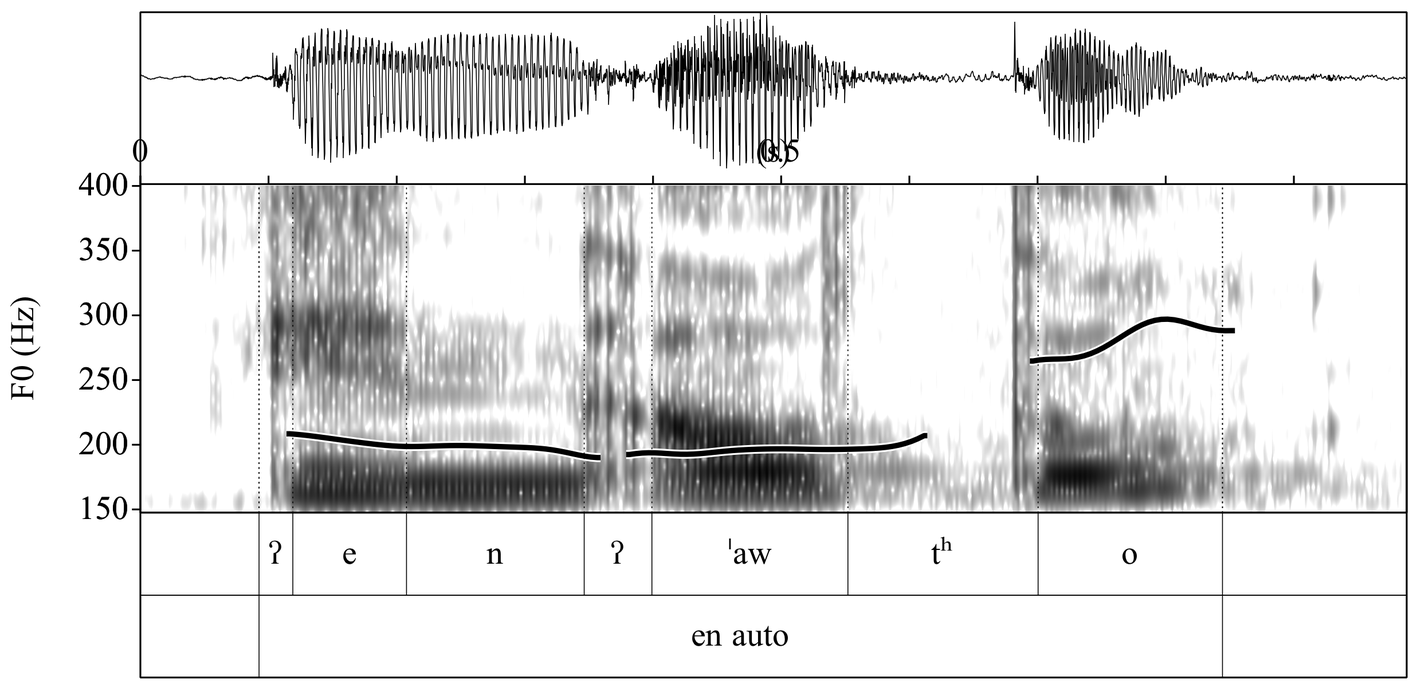
\includegraphics[width=\textwidth]{figures/a02HabilTheory-img013-new.png}



\caption{Insertion of a glottal stop in a C\#V sequence (\textit{en auto}, ‘in the car’) in L2 Spanish produced by an L1 German learner (F\_18).}
\label{fig:2.11}
\end{figure}

Based on this short contrastive analysis and the data gathered in the present study, we can conclude that German learners of Spanish (and potentially of Italian) have more difficulties with the pronunciation of the segments in Romance languages than Czech learners. On the other hand, German shares more prosodic similarities with the Romance languages, as we will see in the next section.

\subsection{Suprasegmental properties in contrast}\label{sec:2.3.2}

As already explained in \sectref{sec:2.2}, intonation serves a variety of linguistic functions such as expressing modality, marking focus and the edges of discourse units, and implementing the lexical accent. In this section, which begins with the presentation of the prosodic typology (\sectref{sec:2.3.2.1}), I will give an overview of other prosodic resources that can also be used to encode these linguistic features and/or are connected directly or indirectly with the use of F0 (\sectref{sec:2.3.2.2}--\sectref{sec:2.3.2.3}). Then, I will present the main tonal patterns of the four languages studied here (\sectref{sec:2.3.2.4}). A summary of their main prosodic features is given in \tabref{tab:2.6a}.

\begin{sidewaystable}
\begin{tabularx}{\textwidth}{QQQQQ}

\lsptoprule

{Prosodic features} & \multicolumn{2}{l}{{Target languages}} & \multicolumn{2}{l}{{L1 backgrounds}}\\
\cmidrule(lr){2-3}\cmidrule(lr){4-5}
& {Italian} & {Spanish} & {Czech} & {German}\\
\midrule
\multirow[t]{2}{=}{Prosodic typology (\citealt{Féry2017, Jun2014})} & {Intonation} language & {Intonation} language & {Phrase} language & {Intonation} language\\
& Head-prominence language & Head-prominence language & Head\slash edge-prominence language & Head-prominence language\\
\tablevspace
Word-stress & Distinctive lexical stress & Distinctive lexical stress & Delimitative stress (fixed on the first syllable) & Distinctive lexical stress\\
\tablevspace
\multirow[t]{2}{=}{Acoustic correlates of stress

(example of pitch track in isolated words)} & Duration, F0, intensity & F0, duration, intensity & No clear correlates & F0, duration, intensity\\
 & 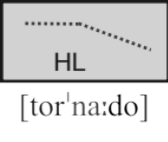
\includegraphics[width=.15\textwidth]{figures/a02HabilTheory-img014.png} & 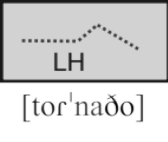
\includegraphics[width=.15\textwidth]{figures/a02HabilTheory-img015.png} & 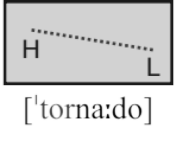
\includegraphics[width=.15\textwidth]{figures/a02HabilTheory-img016.png} & 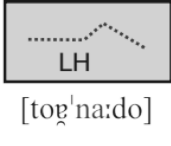
\includegraphics[width=.15\textwidth]{figures/a02HabilTheory-img017.png}\\
\midrule
\end{tabularx}
\caption{Main suprasegmental features of Italian, Spanish, Czech and German in contrast.}
\label{tab:2.6a}
\end{sidewaystable}
\begin{sidewaystable}\ContinuedFloat
\begin{tabularx}{\textwidth}{QQQQQ}

\midrule

{Prosodic features} & \multicolumn{2}{l}{{Target languages}} & \multicolumn{2}{l}{{L1 backgrounds}}\\
\cmidrule(lr){2-3}\cmidrule(lr){4-5}
& {Italian} & {Spanish} & {Czech} & {German}\\
\midrule
Rhythmic isochrony\footnote{The notion of rhythm refers here to the perceptual difference resulting from the isochrony of speech intervals. In very simple terms, syllables in syllable-timed languages tend to have equal duration, whereas intervals between two stressed syllables are equal in stress-timed languages (\citealt{Abercrombie1967} and \citealt{Pike1945}). Spanish and Italian are usually classified syllable-timed languages, whereas German is a stress-timed language (see, e.g., \citealt{Dauer1983, RamusEtAl1999, GrabeLow2002, WhiteMattys2007}), albeit rhythmic characteristics may be less clear cut as shown by, for example, the recent study by \citet{DImperioEtAl2020} for Italian (for criticism or alternative proposals to this traditional isochrony of the rhythm, see, e.g., \citealt{Arvaniti2009}). The rhythm type of Czech has so far not been resolved. \citet{DankovičováDellwo2007} have suggested that Czech is a kind of mixed-stressed language, mainly due to the existence of a contrast between long and short vowels and the syllable complexity that are typical of stress-timed languages.} & Syllable-timed language & Syllable-timed language & {Mixed-timed}

 language & Stress-timed language\\
 \tablevspace
\multirow[t]{2}{=}{Macro-rhythm and tonal density \citep{Jun2014}} & Strong & Strong & Strong(?) & Medium\\
& Dense pitch accent distribution & Dense pitch accent distribution & {Sparer pitch}

 accent distribution & Sparer pitch accent distribution \\
\lspbottomrule
\end{tabularx}


%\caption{Main suprasegmental features of Italian, Spanish, Czech and German in contrast (continued).}
%\label{tab:2.6b}
\end{sidewaystable}

\subsubsection{Prosodic typology and prominence}\label{sec:2.3.2.1}
\begin{sloppypar}
All languages use pitch variation in a meaningful way, but they differ in how pitch is employed for linguistic purposes. Following \citegen{Féry2017} typology, at least four types of languages are distinguished. \textit{Tone languages} (e.g., Chinese Mandarin) make contrastive use of pitch at the lexical level: tones change the meaning of individual words. Tones in \textit{intonation languages} (e.g., English) are specified at higher prosodic levels. As explained in \sectref{sec:2.2}, pitch is used post-lexically for grammatical or pragmatic purposes; in other words, the same sentence can be pronounced with different ``melodies'' according to its function in a discourse. Languages that combine lexical and intonational uses of pitch are called \textit{pitch} \textit{accent languages} (e.g., Swedish). Finally, \textit{phrase languages} (term introduced by \citealt{Féry2010}) share most characteristics with intonation languages, but they also assign phrasal tones (e.g., French).\footnote{Phrasal tones are tones assigned at the level of what \citet{Féry2017} calls a Prosodic phrase (φ phrase), which usually consists of minimally one prosodic word and “that is more or less isomorphic to syntactic phrases, as for instance noun phrases, prepositional phrases or verb phrases” (p. 323). Prosodic phrase is also called Accentual phrase (AP) in the literature (e.g., \citealt{Jun2005, Meisenburg2011}); this term will also be applied in the present study. I will pursue this point later.} This type is very typical for languages with fixed or no lexical stress. Italian, Spanish and German (lexical stress languages) are all prototypical intonation languages, even though they differ from each other, for example, in tonal inventories and in semantic\slash pragmatic meanings of tonal events. As for Czech (a fixed-stress language with initial prominence), it has been proposed that it belongs to phrase languages (\citealt{Pešková2017, PeškováEtAl2018}).
\end{sloppypar}


This typology of language can be further refined according to certain additional criteria. In her model of a prosodic typology, \citet{Jun2005, Jun2014} applies prominence type (head, edge, head/edge) as one parameter for classifying languages.\footnote{This typology of language can be further refined according to certain additional criteria. In her model of a prosodic typology, \citet{Jun2005, Jun2014} applies prominence type (head, edge, head/edge) as one parameter for classifying languages (see \sectref{sec:2.3.2}).} According to this approach, Italian, Spanish and German are \textit{head-prominence languages}, marking phrase-level prominence by the phrase head, which is determined by a metrically strong syllable. This means that a stressed syllable as the head of a word is very important for the anchoring of intonational excursions or pitch accents in all these languages. By contrast, Czech can be seen as a \textit{head/edge-prominence language}, where phrase-level prominence is marked by both, the phrase head and the edge of a phrase. Hence, the main contrast between the two language categories is that a head-prominence language assigns pitch accents associated with stressed syllables, whereas a head/edge-prominence language marks prominence not only with pitch accents but also with boundaries at the phrase level, corresponding to an accentual phrase (AP). Similar to what we see in French, an AP is considered the smallest prosodic phrase (with a break index 2), dominated by an intermediate or intonational phrase. So far there is no broad consensus about the exact characteristics of the AP in Czech, but following \citet{PeškováEtAl2018} and \citet{PeškováForthcoming} we can make at least two main assumptions.\footnote{It can be added that traditional and/or earlier works on Czech intonation (see, e.g., \citealt{Mathesius1937, Ondráčková1954, Palková2017}) call such accentual phrases ``rhythmic'', ``melodic'' or ``speech'' groups/units, which are typical for rhythmic structuring of Czech speech.} First, this small prosodic unit corresponds to at least one lexical word and to all the function words that this lexical word governs (compare with French in \citealt{Delais-RoussarieEtAl2015}). The boundaries of AP generally correspond to syntactic phrases (an in-depth analysis of prosodic phrasing is still required, however). Second, in statements, the stressed syllable is realized mostly with a low pitch level, analysed as L*, and a boundary tone at the edge of the AP with a high peak (Ha) (see an example for Czech in \figref{fig:2.12}). In contrast, the high tones in head-prominence languages such as Spanish or Italian are (mostly) associated with stressed syllables but not the boundary (see an example for Italian in \figref{fig:2.13}).




\begin{figure}
%%\includegraphics[width=\textwidth]{figures/a02HabilTheory-img018.tif}
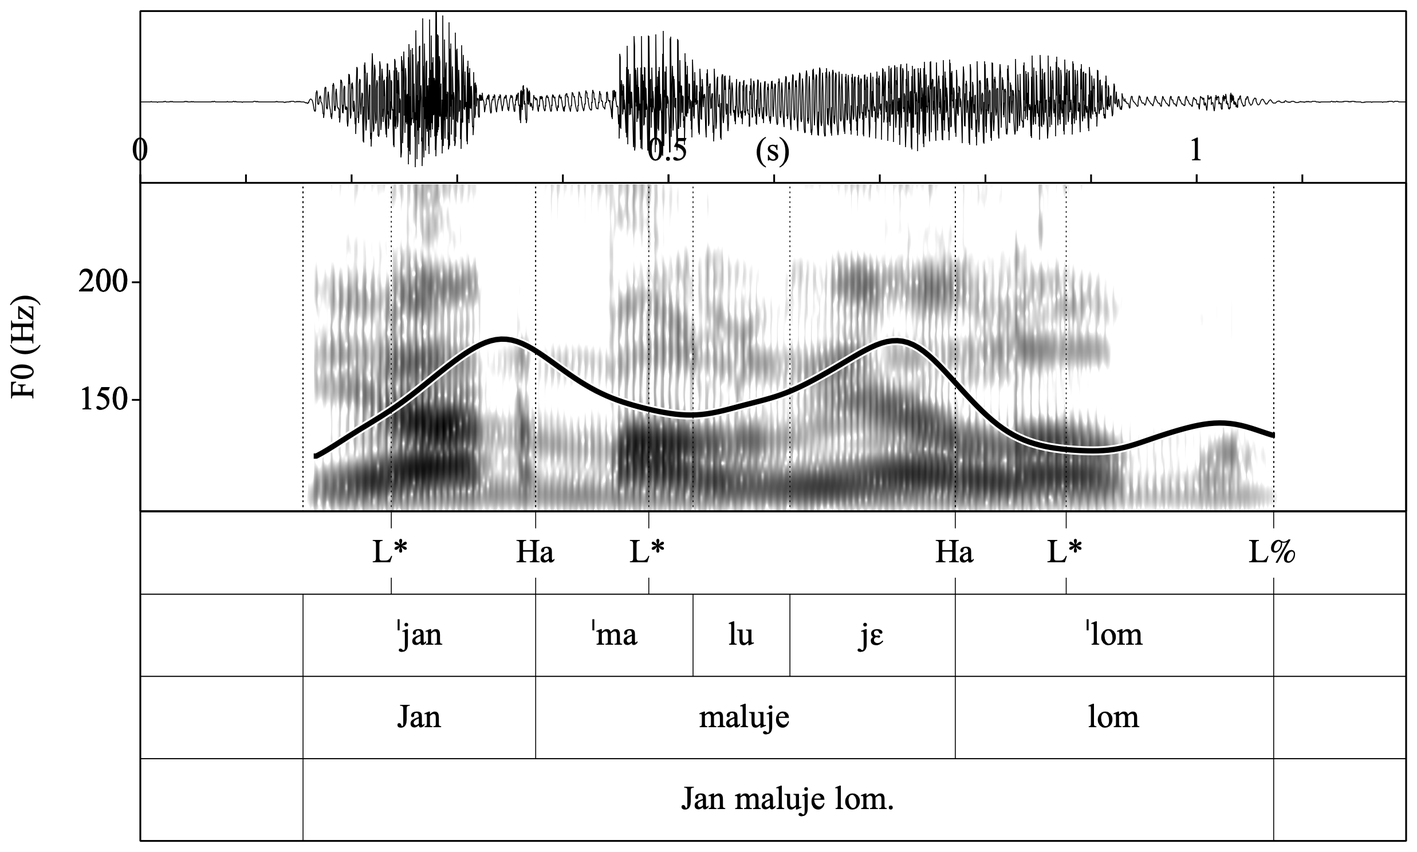
\includegraphics[width=\textwidth]{figures/a02HabilTheory-img018-new.png}



\caption{Waveform, spectrogram, and F0 contour of the broad focus statement \textit{Jan maluje lom} ‘Jan paints a quarry’ in L1 Czech (from \citealt{PeškováForthcoming}).}
\label{fig:2.12}
\end{figure}



\begin{figure}
%%\includegraphics[width=\textwidth]{figures/a02HabilTheory-img019.tif}
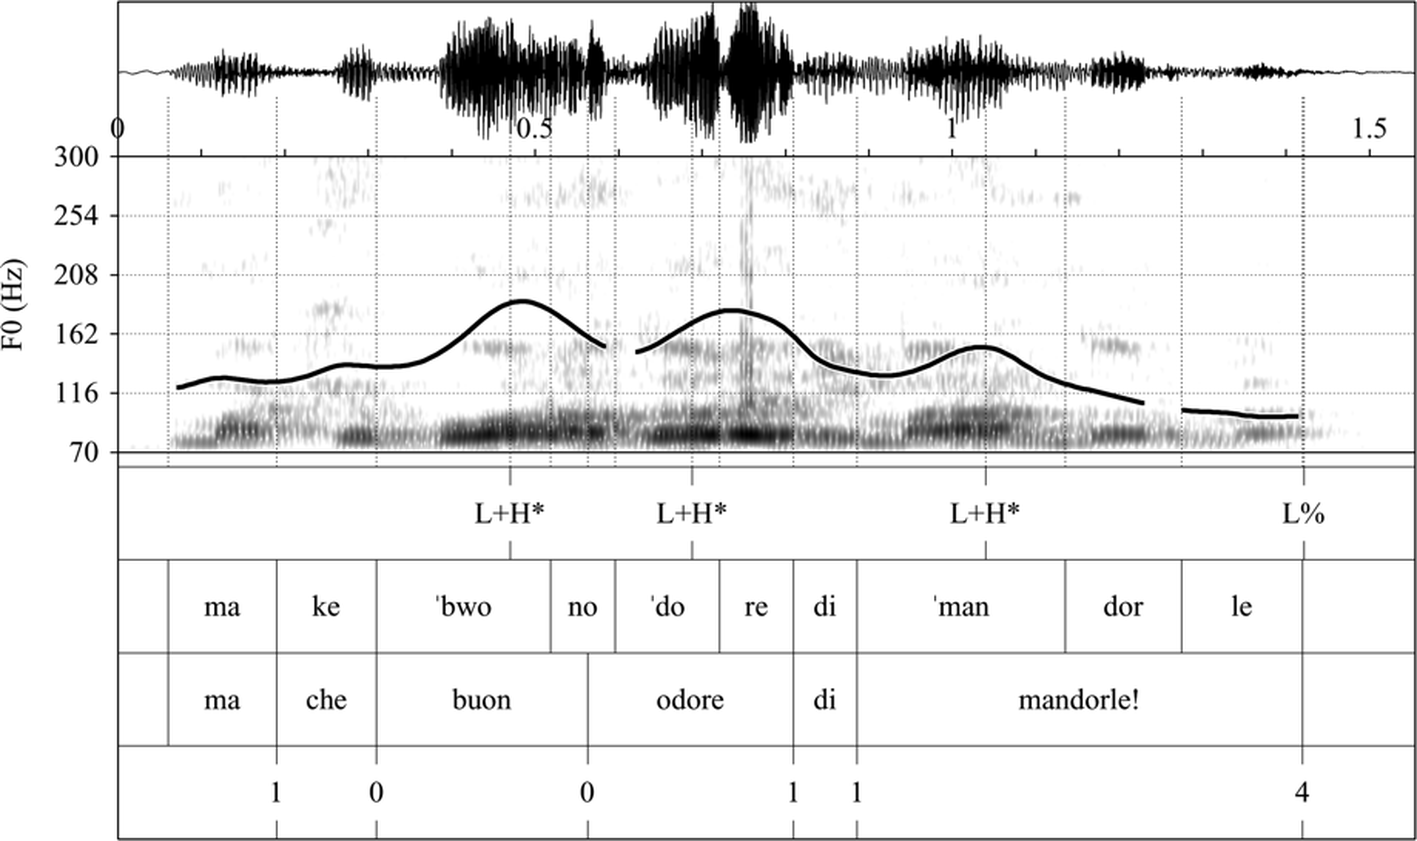
\includegraphics[width=\textwidth]{figures/a02HabilTheory-img019-new.png}



\caption{Waveform, spectrogram, and F0 contour of the exclamative statement \textit{Ma che buon odore di mandorle!} ‘What a good smell of almonds!’ in L1 Italian (from  \citealt[165]{GiliFivelaEtAl2015}, their figure 5.7).}
\label{fig:2.13}
\end{figure}

Interestingly, Czech behaves very similarly to other head/edge-prominence languages such as Bengali (\citealt{HayesLahiri1991, Khan2014}), Tamil \citep{Keane2014} or Hindi \citep{PatilEtAl2008}, which also all have fixed stress on the first syllable. An initial high tone at the very beginning of the utterance is possible, but optional in Czech. Previous work on Czech intonation contemplates additional tonal patterns, including different combinations of L and H tones (see \citealt{Palková1994, Duběda2014}). This variation can be attributed to the number of syllables, expressivity or stylistics, but given the fact that the research on Czech intonation within the AM theory is still in its infancy, further research is still needed in order to fully understand this variation. Considering that the placement of stress plays a role in the prosodic typology introduced above, we will have a closer look at this issue in the following section.

\subsubsection{Lexical stress}\label{sec:2.3.2.2}

All the languages studied here have lexical stress. Stress refers to the degree of relative prominence “that a syllable receives in comparison with the other syllables in a given domain” (\citealt[220]{Hualde2005}, see also  \citealt{GoedemansvanderHulst2013}). Italian, Spanish and German are all lexical stress languages, in which stress has a distinctive function, meaning stress is phonemic and can build minimal pairs (e.g., Sp. [ˈnumeɾo] ‘number’ vs. [numeˈɾo] ‘s/he numbered’). In contrast, Czech is a fixed-stress language, in which stress has a demarcative or delimitative function and is always on the first syllable (e.g., \textit{Praha} [ˈpraha], ‘Prague’). When a monosyllabic preposition precedes a lexical word and both build a single prosodic unit, stress is automatically moved to the very first position (\textit{do Prahy} [ˈdoprahi], ‘to Prague’).


The question is what acoustic correlates are used to convey prominence pattern of the lexical word in the languages under study. German and Spanish use F0 modulation together with duration and/or intensity as important correlates of stress (\citealt{JessenEtAl1995, Jessen1999, Möbius1993} for German;  \citealt{LlisterriBoix1991, LlisterriBoixEtAl2003, Hualde2014} for Spanish). Additionally, German stressed syllables can be identifiable on the basis of the vowel quality too because of vowel reduction in unstressed positions. Whereas F0 appears to be the most significant correlate in Spanish, with duration or intensity as additional strong predictors of stress \citep[245]{Hualde2005}, Italian shows a slightly different picture. The first experimental evidence by \citet{Bertinetto1981} and the results of a recent study by \citet{ErikssonEtAl2016} revealed that duration is the dominant factor of lexical stress in Italian, whereas the role of F0 is secondary. It was also shown that stressed vowels tend to be significantly longer than the corresponding unstressed vowels, regardless of syllable structure. Czech behaves in a very different way from these three languages, exhibiting no clear correlate for stress (\citealt{Volín2010, SkarnitzlEriksson2017}). This might be connected precisely with fixed stress, which is predictable. Interestingly, the posttonic syllable usually receives more prominence -- in the sense of higher values of intensity or a high F0 track. This prominence tends to be sometimes wrongly interpreted as a stressed syllable by foreigners listening to Czech words (\citealt[147]{SkarnitzlEtAl2016}). The first stressed syllable in Czech may also receive such prominence, but this is limited to emphatic or chanted speech and to focus structures (\citealt{SkarnitzlEtAl2016, PeškováForthcoming}, see also \chapref{ch:4}). It could also be suggested that Czech -- similar as, for example, French in some proposals (see, e.g., \citealt{Jun2005, Delais-RoussarieEtAl2015}) -- has not lexical but postlexical stress, meaning that the prominence is assigned to an accentual phrase or other higher prosodic unit. For the time being, I will have to leave this issue unresolved.



Based on the main characteristics of stress, Czech learners usually show more difficulty with the correct placement and/or with the phonetic implementation of stress in Spanish (or Italian) than German learners. An example of this difficulty is given in \figref{fig:2.14} (taken from the data of the reading task carried out for the present study and analysed in \citealt{PeškováEtAl2017}, see \chapref{ch:3}).




\begin{figure}
%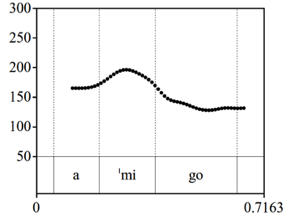
\includegraphics[width=.45\textwidth]{figures/a02HabilTheory-img020.png}
%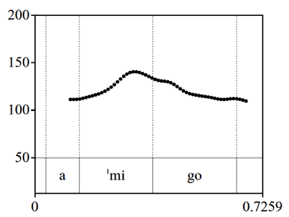
\includegraphics[width=.45\textwidth]{figures/a02HabilTheory-img021.png}




%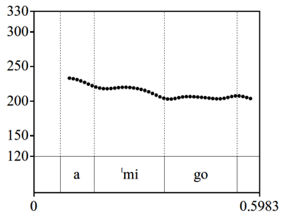
\includegraphics[width=.45\textwidth]{figures/a02HabilTheory-img022.png}
%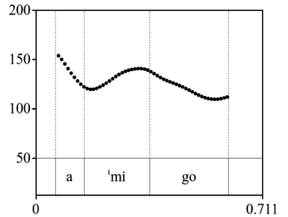
\includegraphics[width=.45\textwidth]{figures/a02HabilTheory-img023.png}
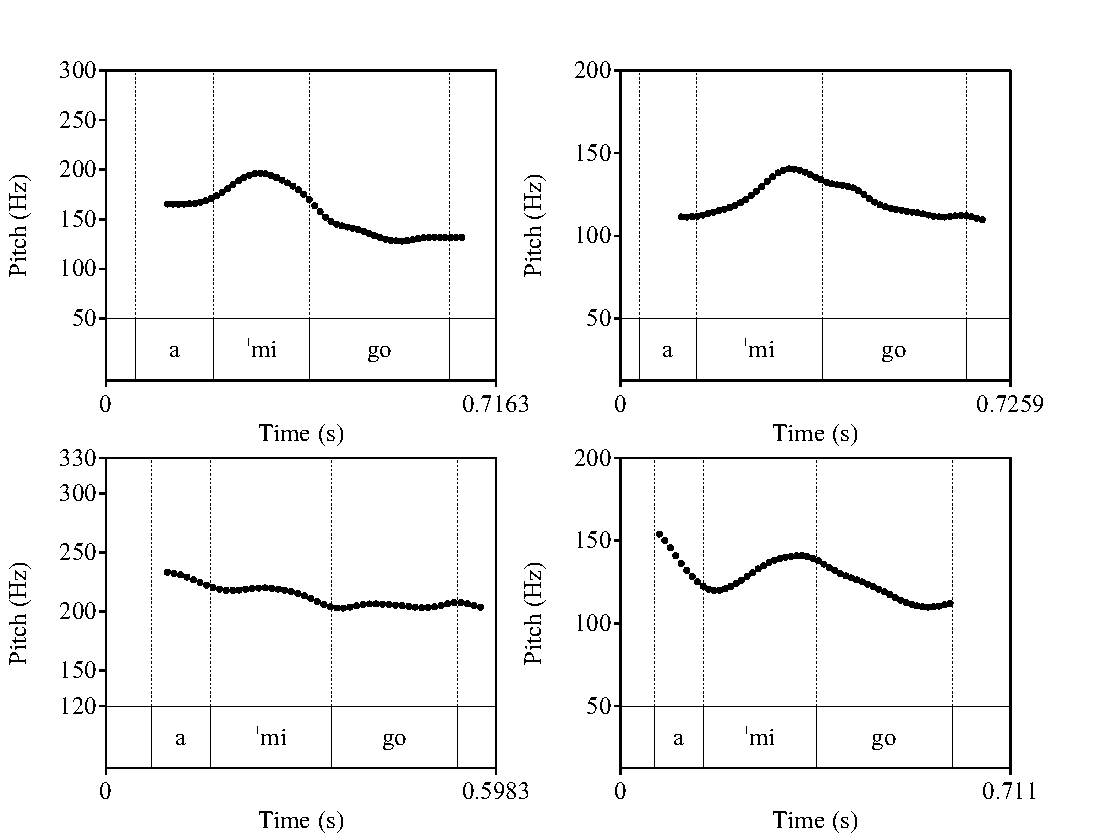
\includegraphics[width=\textwidth]{figures/Figure_2.14.pdf}



\caption{Pitch track of the isolated word \textit{amigo} (‘friend’) in L1 Spanish (at the top left), L2 “German” Spanish (at the top right) and in L2 “Czech” Spanish (below).}
\label{fig:2.14}
\end{figure}

Whereas the German learner of Spanish (\figref{fig:2.14}, picture at the top right) approximates the target pattern (picture at the top left) fairly well, realizing the stressed syllable with a rising F0 movement, the two Czech learners realize it either with a falling pattern from the first syllable or with a target-like pattern and an initial high tone on the first syllable (rightmost picture). Needless to say, such productions were not detected systematically in all Czech learners of Spanish or Italian, but they appeared in the “Czech” L2 data very often and we can therefore call them a typical “Czech” feature. We will see such cases later. Moreover, \citet{PeškováEtAl2017} showed that Czech learners -- especially those at B1/B2 levels -- use durational strategies to express target stress in Spanish, especially when the stressed syllable is not in initial position. Interestingly enough, several Czech words of Spanish origin (see, e.g., \citealt{Ježková2000}) have a long vowel corresponding to the position where the original Spanish word bears stress, as illustrated in \REF{ex:2:1}.


\ea\label{ex:2:1}
\ea \gll {\normalfont Cz.}   \textit{armáda}   {\normalfont /ˈarmaːda/} \normalfont‘army’\\
Sp.   \textit{armada}   /aɾˈmaða/   ‘army’\\


\ex \gll  {\normalfont Cz.}   \textit{kapitán}   \normalfont/ˈkapitaːn/  \normalfont‘captain’\\
Sp.   \textit{capitán}   /kapiˈtan/   ‘captain’\\


\ex  \gll {\normalfont Cz.}   \textit{torpédo}   \normalfont/ˈtorpɛːdo/  \normalfont‘torpedo’\\
Sp.   \textit{torpedo}   /toɾˈpeðo/   ‘torpedo’\\


\ex \gll {\normalfont Cz.}   \textit{generál}   \normalfont/ˈɡɛnɛraːl/   \normalfont‘general’\\
Sp.   \textit{general}   /xeneˈɾal/  ‘general’\\
\z
\z

However, still unanswered are the questions of whether this lengthening is a product of perception or production and why it does not occur with other Spanish borrowings.


The durational effects of stress and syllable complexity together with vowel quantity and quality appear to influence also the speech rhythm of a given language.


\subsubsection{Macro-rhythm and tonal density}\label{sec:2.3.2.3}

Another view on rhythmic properties of languages is proposed by \citet{Jun2014}. She introduces the term \textit{macro-rhythm} and defines it as a tonal rhythm formed within a larger prosodic unit such as an Intonation Phrase. Macro-rhythm together with type of prominence and word prosody represents an important parameter for prosodic typology. Macro-rhythm as a perceived rhythm brought about by changes in F0 differs from \textit{micro-rhythm}, the traditional speech rhythm (see \tabref{tab:2.6a}), which is created by repeated sequences of syllables or feet and which -- according to \citet{Jun2014} -- does not play a role in intonational phonology. \figref{fig:2.15} illustrates the relationship between macro- and micro-rhythm.



\begin{figure}
%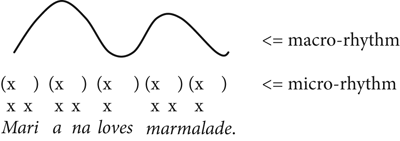
\includegraphics[width=.7\textwidth]{figures/a02HabilTheory-img024.png}
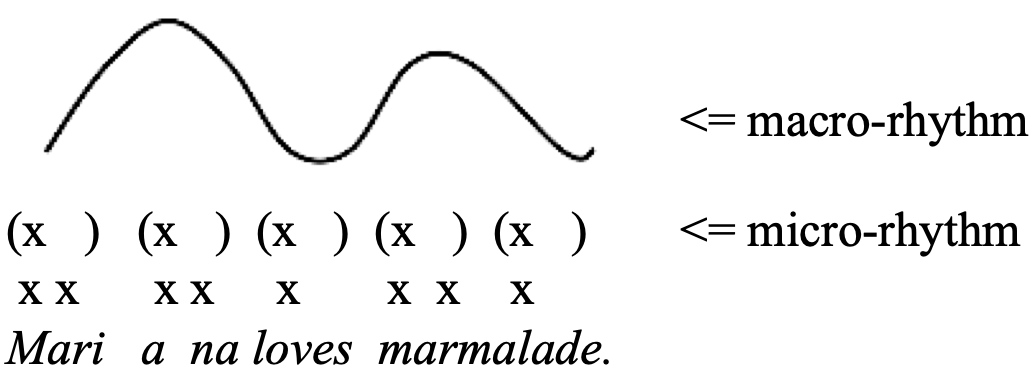
\includegraphics[width=.6\textwidth]{figures/Figure_2.15.png}
\caption{Macro-rhythm and micro-rhythm of the English sentence \textit{Mariana loves marmalade} according to \citet[524]{Jun2014}.}
\label{fig:2.15}
\end{figure}

As explained above, macro-rhythm refers to pitch regularity or repetitions of tonal sequences; fundamental frequency thus contributes to the perception of rhythm in a language and can facilitate word segmentation. Languages differ in the density or sparseness of pitch events in the intonational contour (see also \citealt{Hellmuth2007, FrotaPrieto2015}); in other words, they can exhibit strong, medium or weak macro-rhythm. \citet[525]{Jun2014} proposes three criteria for predicting the degree of macro-rhythm:

\begin{enumerate}[label={(\arabic*)}]\sloppy
\item The \textit{number} of possible phrase-medial pitch accents (PA) or accentual phrases (AP): if a language has fewer alternating types of PA or AP, it is more macro-rhythmic than a language with more variable pitch contours (\figref{fig:2.16}).


\begin{figure}[H]

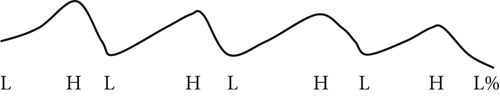
\includegraphics[width=.45\textwidth]{figures/a02HabilTheory-img025.png}
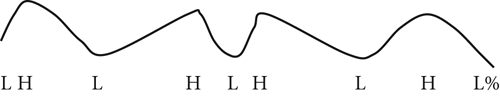
\includegraphics[width=.45\textwidth]{figures/a02HabilTheory-img026.png}


\caption{Stronger macro-rhythm (left) vs. weaker macro-rhythm (right) (from \citealt[525]{Jun2014}).}
\label{fig:2.16}
\end{figure}

\item The \textit{type} of most common PAs or APs: if a language exhibits more rising (LH) or falling (HL) patterns, it is more macro-rhythmic than a language with monotonal levels (H, L) (\figref{fig:2.17}).



\begin{figure}[H]
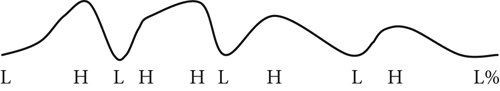
\includegraphics[width=.45\textwidth]{figures/a02HabilTheory-img027.png}
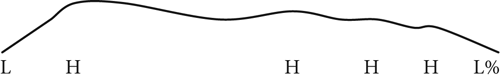
\includegraphics[width=.45\textwidth]{figures/a02HabilTheory-img028.png}




\caption{Stronger macro-rhythm (left) vs. weaker macro-rhythm (right) (from \citealt[525]{Jun2014}).}
\label{fig:2.17}
\end{figure}

\item The \textit{frequency} of PAs and APs: if every word receives PA or AP, then a language is more macro-rhythmic than a language with fewer frequent tonal events (\figref{fig:2.18}).


  \begin{figure}[H]

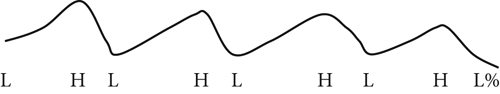
\includegraphics[width=.45\textwidth]{figures/a02HabilTheory-img029.png}
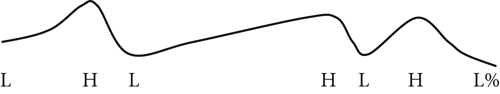
\includegraphics[width=.45\textwidth]{figures/a02HabilTheory-img030.png}




\caption{Stronger macro-rhythm (left) vs. weaker macro-rhythm (right) (from \citealt[525]{Jun2014}).}
\label{fig:2.18}
\end{figure}
\end{enumerate}

According to these criteria, Spanish and Italian are languages with a strong macro-rhythm or a dense pitch accent distribution (\citealt{Jun2014}, see also \citealt{FrotaPrieto2015}), whereas German is a language with a medium macro-rhythm \citep{Jun2014}. Macro-rhythm has not yet been satisfactorily explored for Czech. Nevertheless, the control data collected for this research seem to suggest that Czech also has a strong macro-rhythm (see also \citealt{PeškováForthcoming} for a discussion). Hence, we can conjecture that L2 learners will show more alternations in their production of target pitch accents, precisely because of the differences in the macro-rhythm.


It should be emphasized that \citet{Jun2014} established her typology on the basis of the intonation patterns of declarative sentences described in the literature. And as she notes (\citeyear[539]{Jun2014}), “the degree of macro-rhythm could change if we add other sentence types or include speech materials produced in different styles of speech.” Here further research is needed to quantify macro-rhythm across various languages and data.


\subsubsection{Tonal inventories in contrast}\label{sec:2.3.2.4}

The comparison of intonation patterns serves as a point of departure for the examination of L2 pitch contours in the present study; these are extensively treated in \chapref{ch:4}. Before I start presenting a summary of the main tonal patterns of the languages under study and offering an overview of AM labels used for the annotation of intonational contours, the previous research on intonation is briefly summarized in \tabref{tab:2.7}. Unfortunately, not all work done in this area can be listed here. I have therefore selected only some of them, which also offer important overviews and references for further reading. In general, the research on the intonation of each language under study has a very long tradition, dating back at least to the first half of the 20th century. The earliest of these intonational studies were mostly of a purely descriptive nature based on auditory analysis, but they provide very valuable information on how the ``melody'' of these languages works and sounds like. With the publication of \citegen{Pierrehumbert1980} thesis, interest in intonational phonology spread rapidly and since then the number of studies within the AM framework has greatly increased (some other approaches were mentioned in \sectref{sec:2.2}). It must be noted here that in comparison to Spanish, Italian and German, the modelling of Czech intonation within the AM framework, which started with \citet{Duběda2011, Duběda2014}, is still very limited.

\vfill
\begin{table}[H]
\begin{tabularx}{\textwidth}{lQQQQ}
\lsptoprule
 & \multicolumn{2}{c}{{Target languages}} & \multicolumn{2}{c}{{L1 backgrounds}}\\\cmidrule(lr){2-3}\cmidrule(lr){4-5}
Approach & { Italian} & { Spanish} & { Czech} & { German}\\
\midrule
Non-AM &  \citealt{AgardDiPietro1965, Fiorelli1965, LepschyLepschy1977, DEugenio1982, Canepari1985} &  \citealt{NavarroTomás1948, Quilis1975,Quilis1987} & \citealt{Chlumský1928, Petřík1935a, Petřík1935b, Mathesius1937, Daneš1957,Daneš1985, Grepl1965, Romportl1972, Palková1994,Palková2017} & \citealt{Klinghardt1923, vonEssen1964, Pheby1975, Kohler1991a, Kohler1991b, Fox1984, Selting1995, Peters1999}\\\tablevspace
AM & \citealt{Avesani1990, Grice1995, Rabanus2001, DImperio2002, GriceEtAl2005b, Cangemi2014, GiliFivelaEtAl2015} & \citealt{Sosa1999, Hualde2003, Face2002, FacePrieto2007, BeckmanEtAl2002, AguilarEtAl2009, PrietoRoseano2010, HualdePrieto2015} & \citealt{Duběda2011, Duběda2014, Pešková2017, PeškováEtAl2018, PeškováForthcoming} & \citealt{Féry1993, Grabe1998, Wunderlich1988, Uhmann1991, GriceBaumann2002, GriceEtAl2005a}\\
\lspbottomrule
\end{tabularx}

\caption{Selected works on the intonation of Italian, Spanish, Czech and German.}
\label{tab:2.7}
\end{table}
\vfill\pagebreak

Since the present study was carried out within the AM framework, work undertaken within this approach has been consulted in order to provide the descriptions of tonal sequences. Although we have gained a lot of knowledge about intonation in these languages, research still shows certain limitations (some of the weak points were already discussed in the previous section). First, the proposed (phonological) inventories of tonal patterns (see below) are usually built upon just a few speakers, considering inter-speaker variation to a limited extent (if at all). Second, many studies focus predominantly on the realization of nuclear pitch accents and boundary tones rather than on prenuclear positions, and the “non-phonological” parts between two tonal events are mostly ignored altogether. The reason for not including these parts in the analysis is that they do not convey meaning or do not establish contrasts and are thus less interesting for phonology, in comparison with the nuclear configurations. Though this is certainly true, languages can still differ considerably here and thus “sound” differently. Third, we still lack a comprehensive and “universal” application for the analysis of a large number of (not only dialectal) varieties (the question of regional variation will be addressed below). And, finally, the relationship between F0 and different meanings is still a hot topic too, partly due to the fact that other prosodic cues (intensity, duration etc.) may interact strongly with F0 (see, e.g., \citealt{NiebuhrWinkler2017}).


In spite of these limitations, substantial work has already been done, and the suggested inventories based on acoustic performance allow us to understand the composition of intonation and to compare different tonal patterns within as well as across languages. According to the literature and the intonational analyses contained therein, the tonal inventories of the languages studied here are made up of monotonal and bitonal pitch accents and monotonal and bitonal boundary tones. Tritonal accents represent exceptions. Additionally, Czech as a head/edge-prominence language assigns two types of boundary tones of AP too (Ha, La).\largerpage



\tabref{tab:2.8a} offers an overview of tonal inventories assumed for the languages under study based on previous research. Though the languages have a great deal in common, they differ from each other in how they assign tonal events and in the meanings they convey with these sequences. I will present details in \chapref{ch:4}. At first glance we can see that Spanish and Italian are intonationally “richer” languages in comparison to Czech and German. This concerns in particular the possible combination of pitch accents and boundary tones, called nuclear configurations (NC). (The “rich” inventory of NC in Italian is also due to the range of dialects included here.) As we will see, one nuclear configuration can convey more meanings in every language. For example, in Spanish and Czech, a L* L\% nuclear configuration is found in both (neutral) declaratives as well as in wh-questions (\citealt{Estebas-VilaplanaPrieto2010, Pešková2017}). In Italian, H+L* L\% has a broad range of meanings, including broad-focus as well as narrow-focus statements, exclamatives, wh-questions, or imperative requests (\citealt{GiliFivelaEtAl2015}). And, finally in German, H* L-\% is described for neutral statements and wh-questions (\citealt{GriceBaumann2002}).


\begin{table}[p]
\small
\begin{tabularx}{\textwidth}{QQQQQ}

\lsptoprule

Intonation  & \multicolumn{2}{l}{{Target languages}} & \multicolumn{2}{l}{{L1 backgrounds}}\\
\cmidrule(lr){2-3}\cmidrule(lr){4-5}
inventory\footnote{Sp\_ToBI (\textit{Training materials}) can be found at the following link: \url{http://prosodia.upf.edu/sp\_tobi/en/} (22.6.2019) (cf. \citealt{AguilarEtAl2009}). GToBI (\textit{Übungsmaterialien zur deutschen Intonation}) can be found at the following link: \url{http://www.gtobi.uni-koeln.de/index.html} (22.6.2019) (cf. \citealt{GriceBaumann2002}).} & {Italian}

 (\citealt{GiliFivelaEtAl2015}) & {Spanish}

 (Sp\_ToBI) & {Czech}

 (Cz\_ToBI: work in progress) & {German}

 (G\_ToBI)\\
 \midrule
{Pitch accents} & { L*}

{ H*}

{ H+L*}

{ L+H*}

{ L+<H*}

{ L*+H}

{ L*+>H}

{ H*+L}

{ L+¡H*} & { L*}

{ H*}

{ H+L*}

{ L+H*}

{ L+<H*}

 L*+H & { L*}

{ H*}

{ (H+L*)}

{  (L+H*)\footnote{The phonological status of the L+H* and H+L* in Czech remains unresolved and is discussed in \citet{PeškováForthcoming}.}}

{ L*+H} & { L*}

{ H*}

{ H+L*}

{ L+H*}

{ L*+H}

 H+!H*\\
 \tablevspace
{Boundary tones (AP)} & -- & -- & Ha, La & --\\
\tablevspace
{Boundary tones (ip, IP)} & {L\%}

{ H\%}

{ H!H\%}

{ LH\%}

{ L!H\%}

 HL\% & { L\%}

{ H\%}

{ !H\%}

{ LH\%}

{ L!H\%}

{ HL\%}

 LHL\% & { L\%}

{ H\%}

{ (H)!H\%}

{ LH\%}

{ Hː\%}

 Lː\% & { L\%}

{ H\%}

{ !H\%}

{ LH\%}

 H-\^{}H\%\\
 \midrule
 \end{tabularx}
 \caption{Comparison table for the tonal inventories of Italian, Spanish, Czech and German. The diacritics have the following meaning: \textit{>H*}  indicates H earlier alignment (vs. \textit{<H*} a later alignment), and \textit{\^{}} is another symbol for an upstep.}
 \label{tab:2.8a}
 \end{table}
 
 \begin{table}[p]\ContinuedFloat
 \small
 \begin{tabularx}{\textwidth}{p{.22\textwidth}QQQQ}

 \midrule

 Intonation  & \multicolumn{2}{l}{{Target languages}} & \multicolumn{2}{l}{{L1 backgrounds}}\\
 \cmidrule(lr){2-3}\cmidrule(lr){4-5}
 inventory & {Italian}

  (\citealt{GiliFivelaEtAl2015}) & {Spanish}

  (Sp\_ToBI) & {Czech}

  (Cz\_ToBI: work in progress) & {German}

  (G\_ToBI)\\
  \midrule
{Nuclear

configurations} & { H* L\%}

{ H* LH\%}

{ H*+L L\%}

{ H*+L LH\%}

{ H+L* HL\%}

{ H+L* L\%}

{ H+L* LH\%}

{ L*+>H L\%}

{ L*+H H\%}

{ L*+H HL\%}

{ L*+H L\%}

{ L+¡H* H\%}

{ L+¡H* L\%}

{ L+¡H* LH\%}

{ L+H* H!H\%}

{ L+H* H\%}

{ L+H* L!H\%}

{ L+H* L\%}

{ L+H* LH\%}

 L+H*(+L) L\%\footnote{As stated in  \citet[192]{GiliFivelaEtAl2015}, there are two different realizations of /L+H* L\%/ in Italian, depending on whether the high tone is aligned with the end or with the middle of the stressed syllable. I have used the label L+H*(+L) for the latter case in order to mark this difference. This pattern has been observed in different Italian varieties and in different contexts such as contrastive-corrective narrow-focus statements.} & { H* !H\%}

{ H* HL\%}

{ H* L\%}

{ H+L* HH\%}

{ H+L* HL\%}

{ H+L* L\%}

{ H+L* LH\%}

{ L* HH\%}

{ L* HL\%}

{ L* L!H\%}

{ L* L\%}

{ L* LH\%}

{ L+¡H* L\%}

{ L+H* !H\%}

{ L+H* HH\%}

{ L+H* HL\%}

{ L+H* L\%}

{ L+H* LH\%}

 L+H* LHL\% & { L* (H*) L\%}

{ L*+H (L+H*) L\%}

{ L* (L)H\%}

{ L*+H !H\%}

{ L*+H H\%}

{ L*+H LH\%}

{ L*+H !Hː\%\footnote{In \citet{PeškováEtAl2017}, I argue that the final lengthening (H:\%, L:\%) is phonological in (familiar) exhortative and insistent requests.}}

{ L*+H Lː\%}  & { H* L-\%}

{ H+!H* L-\%}

{ H+L* L-\%}

{ L* H-\^{}H\%}

{ L* L-H\%}

{ L*+H L-\%}

{ L+H* !H\%}

{ L+H* H-\%}

{ L+H* H-\^{}H\%}

{ L+H* L-\%}

 L+H* L-H\%\\
\lspbottomrule
\end{tabularx}
\caption{Comparison table for the tonal inventories of Italian, Spanish, Czech and German (\textit{continued}).\label{tab:2.8b}}
\end{table}

One issue related to the intonation patterns presented should be raised here. The Spanish ToBI is based on Peninsular Spanish, German ToBI on the Northern German spoken variety and Czech ToBI on Moravian and Bohemian dialects, whereas the Italian ToBI illustrates contours of different regional varieties across Italy. Since we know that dialects differ in terms of prosody, the question is how to treat this variation in SLA and L2 classes. In comparison to the acquisition of non-native segments, which can be more easily oriented to the “ideal” (albeit sometimes artificial) native model, the intonation represents a phenomenon that is relatively difficult to “standardize”. Another challenging issue related to the present study was to find participants who had been exposed to a single L2 variety and yet fulfilled also other criteria. This is especially the case of students who have studied an L2 in a classroom in their home country, as is the case of the present study. I will return to this issue in more detail in Chapters~\ref{ch:3}, \ref{ch:4} and~\ref{ch:5}.


Coming back to the tonal patterns presented in \tabref{tab:2.8a}, it must also be added that the tonal inventory for Czech proposed here is preliminary because work on Czech intonation within AM is still in progress. The present proposal does not differ from the Czech intonational grammar suggested in \citeauthor{Duběda2011}’s earlier studies (\citeyear{Duběda2011, Duběda2014}), the only difference consisting of the fact that I treat Czech as a phrase language and assume phonological APs. We also observe that this language exhibits the most limited tonal inventory. On the other hand, it shows a larger phonetic “flexibility” within the AP domain. For instance, the underlying tone /L*+H/ appears to be implemented phonetically as L+H* (or L+<H*), which is subject to the length of a word. Whether there might be a phonological difference between L+H* and L*+H in some instances is not clear so far. Nor is it clear whether H+L* should be included in the tonal inventory. \citet[88]{Duběda2014} incorporates this prenuclear “accentual peak”, consisting of a falling contour between the stressed and the posttonic syllable, into his inventory. In my approach, such falling patterns can be seen as a mere phonetic implementation of L* within a default AP (L* Ha). Furthermore, Czech pitch contours share a lot of phonetic similarities with the other three intonation languages, but for phonological reasons, the same F0 movement is labelled differently. An example is given in Figures \ref{fig:2.19} and \ref{fig:2.20}. Here the nouns \textit{pomeranče} (Czech) and \textit{naranjas} (Spanish) (‘oranges’), which both are in focus, are analysed differently: L*+H (i.e., low tone on the accented syllable and rise on the posttonic syllable) in Czech vs. L+H* (i.e., rising tone on the accented syllable and fall on the posttonic syllable) in Spanish, respectively. But note that the pitch movement of the focus domain is almost the same in that we have here one word with more than two syllables realized with a low pattern on the first syllable (the stressed one in Czech), followed by a sharp rise on the second syllable (the stressed one in Spanish); the last syllable(s) is/are realized with a fall and low tone.\footnote{Notice that the final AP in an ip or an IP does not bear phrasal tones (La, Ha) due to the so called \textit{concurrent boundary tone overriding} (term used in \citealt{Khan2014} for Bengali). This is valid for final accentual phrases.}




\begin{figure}[p]
%%\includegraphics[width=\textwidth]{figures/a02HabilTheory-img031.tif}
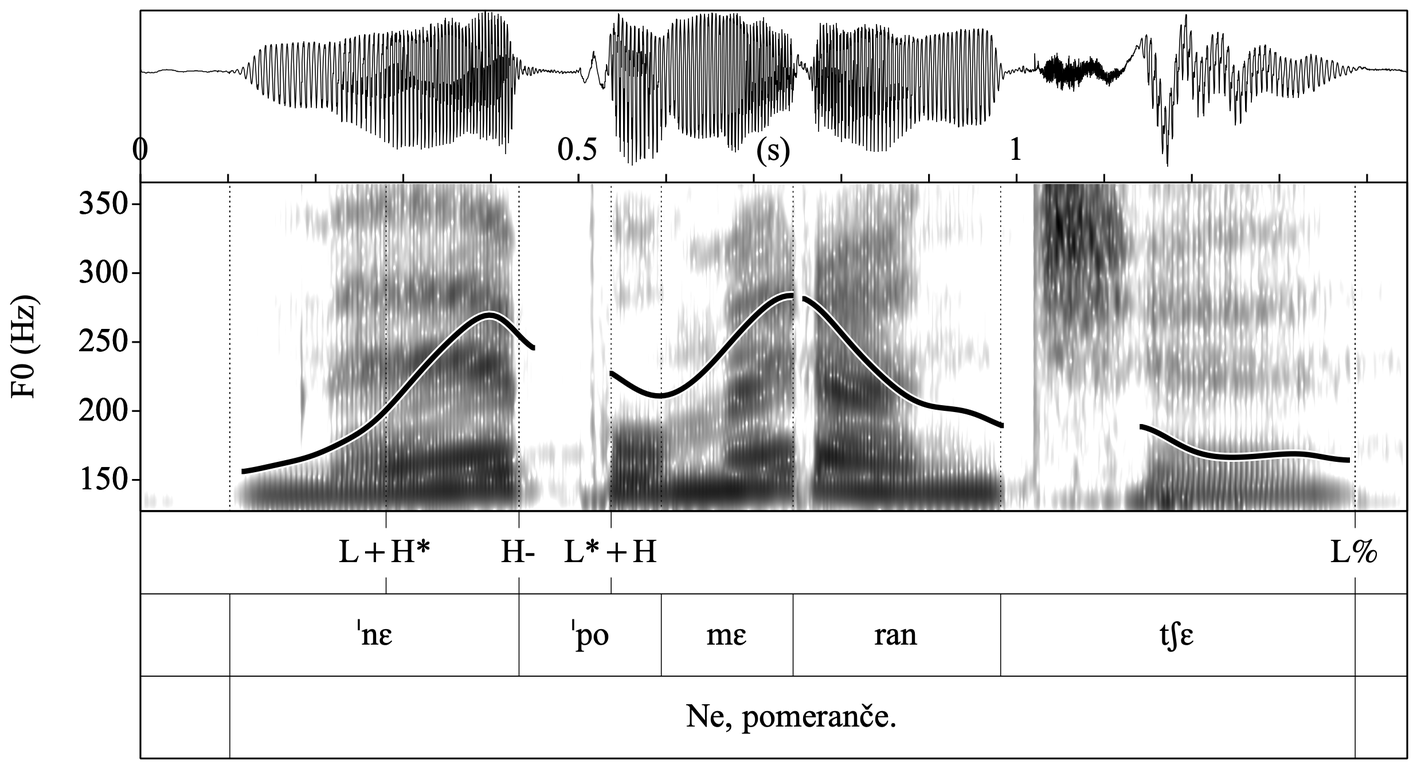
\includegraphics[width=\textwidth]{figures/a02HabilTheory-img031-new.png}
\caption{Focus marking in a narrow focus statement \textit{Ne, pomeranče!} (‘No, oranges!) in L1 Czech.}
\label{fig:2.19}
\end{figure}


\begin{figure}[p]
%%\includegraphics[width=\textwidth]{figures/a02HabilTheory-img032.tif}
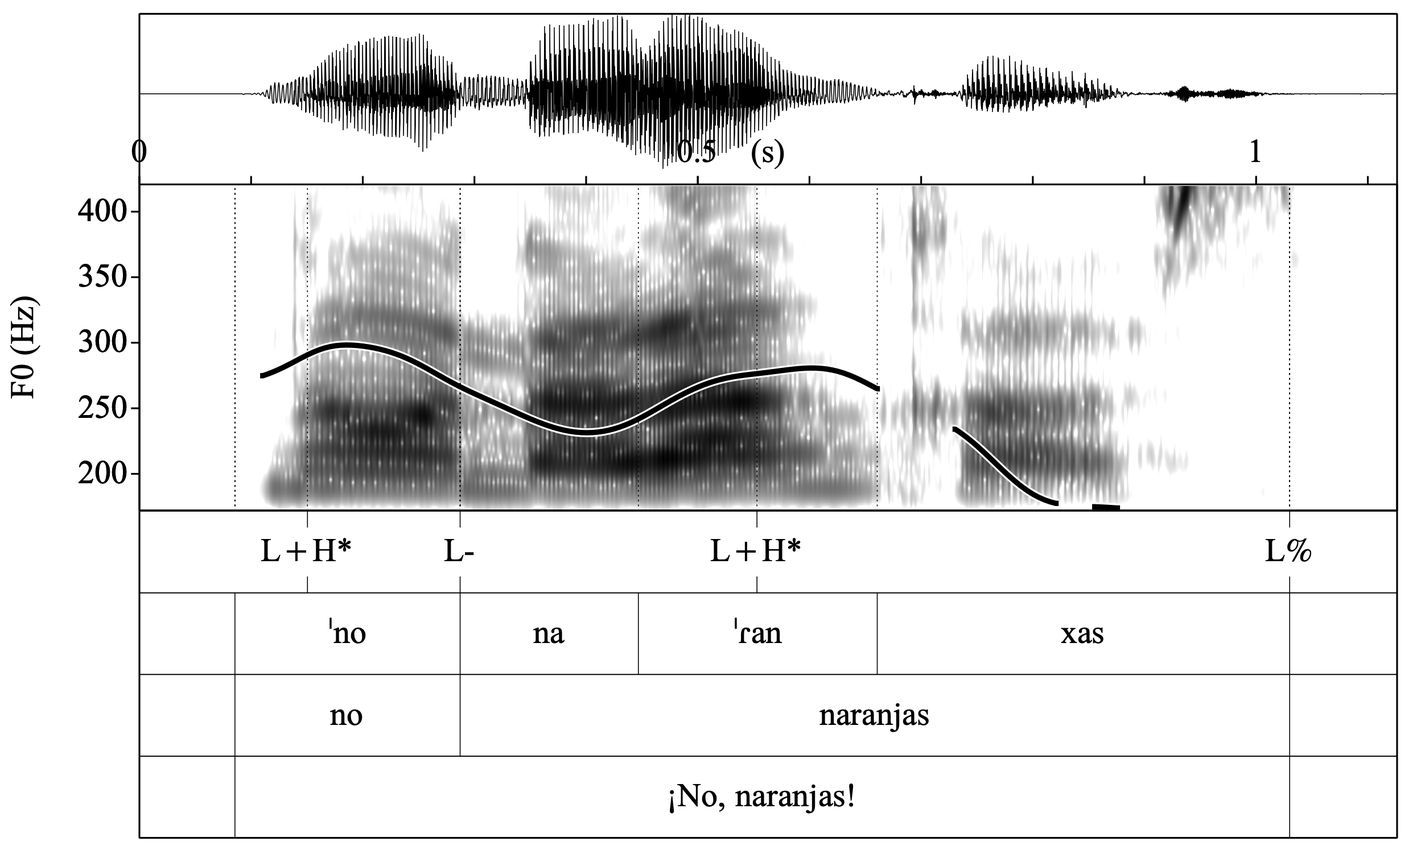
\includegraphics[width=\textwidth]{figures/a02HabilTheory-img032-new.png}

\caption{Focus marking in a narrow focus statement \textit{¡No, naranjas!} (‘No, oranges!) in L1 Spanish.}
\label{fig:2.20}
\end{figure}

In sum, all languages can display contours that are phonetically the same but phonologically different; and the other way round, they can have contours that may be phonologically the same but phonetically different.


With reference to the tonal inventories presented above and findings reported in the previous research, we can expect CLI in L2 productions. The central question is which (if any) tonal targets are produced in a target-like manner and which features from L1 are transferred in L2 and why. These issues are considered properly in the fourth chapter, which describes intonation patterns according to four -- both neutral and non-neutral -- sentence types (declaratives, yes/no questions, wh-questions and vocatives) and formulates hypotheses based on similarities and dissimilarities seen across the languages under study. Before coming to the results regarding intonation patterns in L2 Italian and L2 Spanish in \chapref{ch:4}, in the section that follows I present various theoretical approaches and proposals related to modelling of L2 speech and L2 intonation.


\section{Models of L2 speech acquisition}\label{sec:2.4}
\largerpage
Up to now, it was explained what L2 speech means and which goals research on L2 speech pursues, what factors may shape a foreign accent and explain individual learner differences (\sectref{sec:2.1}), how intonation is defined and modelled (\sectref{sec:2.2}), and, finally, in which ways the languages under study differ in terms of segmental and suprasegmental phonology (\sectref{sec:2.3}). This section presents and discusses various theories and models that have attempted to interpret CLI and to predict what kinds of difficulties or errors occur in non-native speech. Many theoretical proposals have been put forth, both production-based and perception-based, and it will not be possible to cover all of them here. Rather, this attempt to come to a closer understanding of the processes in L2 acquisition will be grounded in a limited selection of approaches (for overviews as well as discussions of the different theoretical approaches, see, e.g., \citealt{Eckman2004, ColantoniEtAl2015, DerwingMunro2015}). Since the present study deals with L2 intonation, I find of particular interest \citegen{Mennen2015} \textit{L2 Intonation Learning theory}, which is based on the AM framework fundamental to the present study. Before introducing the LILt in \sectref{sec:2.4.2}, I will establish a foundation with contrastive analysis.


\subsection{Contrastive analysis}\label{sec:2.4.1} %2.4.1 /
\largerpage
It could be said that modern research on the role of cross-linguistic influences started with two seminals books, \citegen{Weinreich1953} \textit{Languages in Contact} and \citegen{Lado1957} \textit{Linguistics Across Cultures.} Whereas the first of these texts made an important contribution to the role of L1 in L2 in research on contact linguistics and linguistic change, the second laid the groundwork for the theoretical contrastive study of languages with important implications for teaching. Lado’s \textit{Contrastive Analysis Hypothesis} (CAH) suggests working procedures to carry out the systematic comparison of the L1 and L2, including sound systems, grammatical structures, vocabularies, on one hand, and writing systems and cultures, on the other. The systematic comparison of the two languages makes it possible to predict learning difficulties and to show where improvement is needed. One of the central assumptions of the CAH is that learners will have much more difficulty producing and perceiving anything that is “new”. Taking an example from a comparison of sound systems, Lado says that learners will have more problems distinguishing and reproducing sounds that do not exist in their L1s than with sounds that are already present in their L1s.\footnote{\citet[51--52]{Trubetzkoy1969} in his \textit{Principles of Phonology} describes the process of L2 learning in a similar way; he calls it “false evaluation of the phonemes of a foreign language.” According to him, “[e]ach person acquires the system of his mother tongue. But when he hears another language spoken he intuitively uses the familiar ‘phonological sieve’ of his mother tongue to analyse what has been said. However, since this sieve is not suited for the foreign language, numerous mistakes and misinterpretations are the result. The sounds of the foreign language receive an incorrect phonological interpretation since they are strained through the ‘phonological sieve’ of one’s own mother tongue.”} This generalization provoked broad debate and was repeatedly refuted by posterior studies offering evidence that new sounds do not always present difficulties for L2 learners (see, e.g., \citealt{Flege1987, Flege1995, Brown1998}). As for prosody, Lado formulates the following difficulty with regard to the learning of L2 intonation: when the L1 has many levels of pitch (Lado calls them \textit{pitch phonemes}), it is easier to learn a language that contains fewer. With regard to intonation patterns (a set of pitch phonemes within a phrase) in particular, he concludes: “Most of the intonation problems stem from patterns which are the same in form in the two languages but have a different meaning in each” \citep[44]{Lado1957}. This is what \citet{Ladd1996, Ladd2008} and \citet{Mennen2015} call the \textit{semantic} \textit{dimension} (I will come to this issue later). Lado’s generalization holds especially true for a comparison of two intonation languages. According to him, native speakers of tonal languages will have greater difficulty learning intonation languages than tonal languages, just as will native speakers of intonation languages learning a tonal language. Here too, however, research suggests that this need not always be the case. For example, the study on L2 English intonation by \citet{Ortega-LlebariaColantoni2014} showed that Spanish learners transferred more L1 patterns and produced somewhat “worse” English focus marking than (Mandarin) Chinese learners did. The CAH thus seems to be untenable in certain respects. \citet[64--65]{DerwingMunro2015} summarize the weaknesses of the CAH in four points: (1) the CAH does not treat perception and production separately, (2) it does not account for changes in interlanguage over time, (3) it does not explain individual learner differences and (4) it does not clarify the underlying cognitive processes that lead to pronunciation errors. Posterior models and theories have focused especially on the interrelation between production and perception, since perception has been shown to be crucial for both L1 and L2 acquisition of sound systems in general. Moreover, it has been proved that L2 learners also have “perceptual foreign accents”, meaning that learners perceive TL sounds differently than natives of this language do (\citealt[22]{Strange1995}, see also \citealt{McAllister1997}). Nonetheless, in spite of the CAH’s weaknesses, contrastive (and comparative) analysis \textit{per se} still plays a crucial role in different areas of theoretical as well as applied linguistics. After all, it appears to be what (especially adult) learners tend to do as soon as they start to learn a new language: they compare it with their L1 and notice divergent features -- at least the most marked ones. To date, various approaches, both theoretical and empirical, that involve contrastive, error or interlanguage analysis have been set out. Of particular note within second language learning is the method called \textit{Contrastive Interlanguage Analysis} (CIA), introduced in 1996 by Granger for purposes of learner corpus research with a main focus on English as L2 (for a revision of the model, see also \citealt{Granger2015}). As already mentioned in the \textit{Introduction}, I chose this design method because it combines a comparison of non-native and native speakers of a language, on one hand, and a comparison of non-native speakers of a language with different L1 backgrounds on the other. What is new in my study is an additional scenario: a comparison of non-native speakers with the same L1 background who are learning different TLs.



Since the main focus of the present research is on the production of intonation patterns, I will follow \citegen{Mennen2015} \textit{L2 Intonation Learning theory} (LILt), which considers several generalizations from perception- and production-based theories in order to explain the principles which govern the acquisition mechanisms of intonation.


\subsection{L2 Intonation Learning theory \citep{Mennen2015}}\label{sec:2.4.2}

The main motivation behind this theory, which is based on the AM model, is twofold, namely that L2 learners exhibit CLI in L2 intonation, even at a very advanced level, and that research and models of L2 speech have limited utility for the production and perception of segmental phenomena. The LILt provides first a cross-language comparison that allows the identification of L2 intonation “errors” (see \sectref{sec:2.4.2.1}) and then general theoretical assumptions which incorporate different models of L2 (segmental) speech and adjust them to the acquisition of L2 intonation (see \sectref{sec:2.4.2.2}).


\subsubsection{Cross-language comparison and the identification of L2 intonation deviations}\label{sec:2.4.2.1}

Cross-language (and cross-varietal) comparison is the first step assumed in the use of the LILt method. The researcher must describe the L1 intonation patterns and then compare them with L2 intonation patterns, taking into account four central dimensions of cross-linguistic variation, namely the (1) systemic, (2) phonetic, (3) semantic and (4) frequency dimensions (cf. \citealt{Ladd1996,Ladd2008}). Once this comparison is carried out it is then possible to predict where L2 intonation deviations are likely to occur and identify them accurately.



Regarding the first -- systemic -- dimension (inventory and distribution of categorical phonological elements), Spanish and Italian have rich intonation systems and exhibit more different types of pitch accents and boundary tones than German and Czech (see \tabref{tab:2.8a} in \sectref{sec:2.3.2.4}). For example, Spanish LHL\% boundary tones or Italian H*+L and L*+>H pitch accents do not appear in Czech and German at all. The languages also permit different combinations of tonal events. There are clearly more nuclear configurations in the two Romance languages, meaning that these languages use more tones to convey different meanings (we will come to the semantic dimension below). By contrast, Czech and German may either be intonationally ambiguous or compensate for “missing” patterns with other prosodic or syntactic strategies or the use of lexical items such as particles or adverbs. It should be added that Czech also uses further devices for the expression of biased sentences instead of intonation or lexical items, such as different ways of articulation of the segments or changes in F0 span and level (the latter strategies are based on my impressionistic observation and native intuition and deserve systematic investigation in future). It should be added that across and within languages, some sentence types (e.g., narrow focus statements) show tonal consistency, whereas other sentence types (e.g., yes/no questions) display high variation. The four languages under study here differ in their tonal inventories (see, e.g., \citealt{FrotaPrieto2015} for various Romance languages) and we will deal with this and other dimensions properly in \chapref{ch:4}, when results on L2 Spanish and L2 Italian intonation patterns will be reported. At least two questions related to this dimension arise: \textit{Will L2 learners omit those pitch accents and boundary tones that do not form part of their native language inventory? Will they transfer their native patterns that are not present in the target language}? For example, \citet{Mennen2015} reports that neither Italian nor Punjabi learners of the same variety of English produce complex pitch accents H*LH and L*HL, which are present in the L2 in question but absent in their respective L1s.\largerpage



With regard to the second (phonetic or realisational) dimension, the four languages also differ in how tonal tunes are phonetically implemented. Most importantly, this dimension refers to the realization of the tonal alignment, tonal scale and tonal slope. For example, Spanish shows a high sharp final rise in yes/no questions, which reaches a very high frequency in the speaker’s range, in comparison to Czech or Italian. Originally, Sp\_ToBI proposed the label HH\% for this type of a very high rising movement, which was later changed to a “simple” monotonal H\% (\citealt{PrietoRoseano2010}). Another example is the realization of rising accents in prenuclear positions of broad focus statements (and further possible types of utterances too). Italian and German exhibit mostly an earlier peak alignment within the stressed syllable, whereas Spanish has delayed peaks. In Czech, a phrase language, the situation is slightly different. For example, when the AP is mono- or disyllabic, it has an earlier alignment (within the stressed syllable), and when it has three or more syllables, the rise is aligned with the posttonic syllable or later. So here the question is: \textit{Will learners have particular problems with realization of target-like scaling or alignment of pitch contours?}\footnote{My study will focus especially on alignment and on pitch change. Measurements of slope properties and other phenomena are left for the future.} For example, \citet{Mennen2004} showed by means of a reading task of declarative sentences that a majority of the Dutch learners of Greek she examined (who all had 12–35 years of experience with the TL) tended to align the prenuclear peak much earlier than native Greek speakers. This finding on deviations in pitch alignment supported evidence elsewhere on the influence on L2 intonation of an L1. \citet{TrofimovichBaker2006} reported similar tendencies in the production of English by Korean adult learners, but revealed that the “erroneous” peak alignment did not contribute to the perception of a foreign accent. Interestingly, peak alignment also played no role in foreign accent in Korean children learners of English in a posterior study by \citet{TrofimovichBaker2007}. In contrast, stress timing, speech rate, pause frequency and pause duration showed effects in accentedness ratings in both studies.



Furthermore, the four languages show significant contrasts in the semantic dimension or functionality of the tunes, meaning that their tonal distribution is not the same. For example, L*+H has been described for the focus domain in Czech, but in Spanish for prenuclear accents of yes/no questions. Wh-questions in Spanish have predominantly falling patterns, but in German they commonly end in rises, depending on their pragmatic status. (Neutral) vocatives in German, Spanish and Italian mostly end in (H)!H\%, whereas Czech allows L\% too. The question this issue raises is thus: \textit{Will learners use intonation to signal certain functions in a TL-appropriate way or will they transfer patterns from their L1?} For example, \citet{MengWang2009} showed that Chinese learners of English had difficulties with the production of the final boundary tones in all sentence types except imperatives and differed significantly from natives. The findings were interpreted as a case of negative transfer resulting from a lack of intonation knowledge and context. Similar evidence supporting cross-linguistic influence has been reported in many other studies; see, for instance, \citet{Reinecke2003} for the acquisition of German intonation by Brazilian native speakers; \citet{Radel2008} for the acquisition of Spanish yes/no questions and statements by German learners; \citet{NavaZubizarreta2009} for L2 acquisition of prosodic focus marking in L2 English by native Spanish speakers; \citet{ColantoniEtAl2016b} for the production and perception of statements and questions by L2 speakers of English with L1 Spanish; or \citet{NicoraEtAl2018} for L2 Italian polar questions produced by Irish English speakers. In all these studies, learners transferred patterns from their L1 and/or did not produce the target patterns correctly, even though such patterns might exist in their L1 too. This means that learners’ phonological/semantic (and pragmatic) awareness is relatively low.



The deviations in the semantic dimension are also closely related to the last, fourth dimension, which concerns frequency. This dimension refers to the fact that even when languages share the same patterns, their use can be more or less common. For instance, \citet{TorreiraFloyd2012} report that pragmatically unmarked patterns for Spanish yes/no questions (L* H\%) are less frequent than circumflex contours (L+¡H* L\%) (cited in \citealt[374]{HualdePrieto2015}). In informal Czech, statements may end in rises, but rises are far less common in comparison to the default falling pattern. The question for this dimension is: \textit{Will learners prefer certain patterns more often, and if so, why?} Unfortunately, we do not have exact and satisfactory information on the frequency of all categorical elements for all the four languages. However, we can assume that deviations in this dimension also arise from cross-linguistic influence \citep{Mennen2015}. For example, a recent study by \citet{GabrielEtAl2018} provides evidence that German learners of French tend to overgeneralize H\% in syntactically and lexically marked interrogatives, where natives also produce L\%. The authors connect this finding with L1-to-L2 transfer effects.



In short, the LILt offers a very useful approach to formulate and test specific hypotheses in identifying L2 intonation patterns. In the next section, I present the general theoretical assumptions on which the LILt rests.


\subsubsection{General theoretical assumptions of the LILt}\label{sec:2.4.2.2}

While cross-language comparison allows us to predict what kinds of difficulties may occur in L2 intonation learning, the following theoretical generalizations seek to explain \textit{why} such difficulties arise. In this context, the LILt is founded on two learning models that treat perception and production separately and focus on the process of L2 acquisition: \citegen{Flege1995} \textit{Speech Learning Model} (SLM) and \citegen{BestTyler2007} \textit{Perceptual Assimilation Model of L2 Learning} (PAM-L2) (see also \citeauthor{Best1994}'s \citeyear{Best1994,Best1995} \textit{Perceptual Assimilation Model}). Based on these two models and on findings from research on the acquisition of L2 segments, the LILt formulates five core theoretical assumptions that are summarized below:\largerpage



\begin{enumerate}[label={(\arabic*)}]
\item
         The first theoretical assumption states that learners’ perception of intonational cues that are not present in their L1 or differ from L1 categories is limited. This implies that the observed deviations in L2 speech production are perceptually motivated. It seems logical to believe that what a learner does not hear, s/he cannot produce. For example, Czech learners of Italian have great difficulty distinguishing [e] from [ɛ], because their vowel inventory accounts only for /ɛ/. However, as observed with other segmental phenomena, learners may fail to correctly articulate other sounds even though they perceive them easily. One example here is the Spanish /r/, which causes considerable trouble for German learners. We can imagine a similar parallel with intonation patterns. However, as Mennen underlines, the existence and perception of categories for intonation is much more difficult to define than categories for segments because variations in intonational form convey both linguistic and paralinguistic meaning. Therefore, the LILt recommends making explicit reference to the semantic dimension of intonation when determining perceptual similarity. In this context it is worth mentioning the empirical study on prosodic focus marking in English by \citet{Ortega-LlebariaColantoni2014}, who found that learners’ perception of focus marking was shaped by their L1 (Spanish) and that the L1 transfer effects increased (in production) when learners were given greater access to meaning (i.e., when a context was added). The present study does not deal with perception data, but the in-depth analysis of production data might help to reconstruct the manner in which learners perceive a foreign intonation. The question is: \textit{Will learners easily acquire tonal patterns in TL that are different from L1 categories?} Based on a very simplified version of Flege’s SLM assumption, L2 new sounds should be easier to acquire than phonetically similar sounds between L1 and L2. For example, a rising tone differing in alignment can cause more difficulty than a tonal pattern that is completely new to learners. According to Flege, perception also plays a central role here: he assumes that if a learner successfully acquires a distinction at the perceptual level, s/he will also be more accurate in production over time.





\item
         The second assumption refers to L1 influences. The LILt posits that they are not restricted to the level of \textit{phonological contrasts}. Even small differences at the phonetic level may influence the perception of foreign accent. Hence, the LILt recognizes that similarities and dissimilarities between L1 and L2 intonation can also occur along the phonetic (and not only systemic) dimension (see \sectref{sec:2.4.2.1}) and that a learner’s ability to discriminate, categorize and produce an L2 phonological category depends on variation in the realisational dimension. Moreover, the LILt argues that the contrasts must be tested and controlled for position and context too.\largerpage



\item
         The third assumption is related to the \textit{Age of Learning} (AOL), which is considered an important predictor of the successful acquisition of a TL (see also \sectref{sec:2.1.3}). The LILt predicts that intonation production will be more successful when learning begins “at a younger age”. In \sectref{sec:2.1.4} we already discussed this factor extensively and concluded that input quantity and quality -- besides a large number of further internal and external factors -- are also involved in AOL and have an impact on L2 speech. All participants in the present study began to learn the L2 at or after puberty (see Chapter 3 for details).



\item
         The fourth postulation deals with \textit{L2 intonation development} over time, and the phenomena that bear on its ultimate attainment, such as fossilization, among other things. The LILt suggests that as learners gain experience in the L2, the production of L2 intonation parameters will approximate target forms more closely. Again, the present study is not longitudinal, but it assumes that L1 transfer will be stronger in intermediate than in advanced learners. In relation to this assumption, the LILt assumes that not all intonation dimensions represent the same degree of difficulty in L2 learning and that individual variation may play an important role.



\item
         And finally, the fifth generalization focuses on evidence that L1 and L2 (phonetic) categories exist in a \textit{common phonological space}. This may lead to interaction between the languages that can take the form of assimilation or merging of L1 and L2 properties (bi-directional interaction can also occur; this is especially true for bilingual speakers and high-level advanced speakers, such as immigrants who have lived in an L2-speaking area for a long time). A simple question that emerges from this generalization is: \textit{Will the learners show more L1 patterns, target-like patterns or L1-L2 mixed patterns?}
\end{enumerate}


To conclude this section, I would like to raise one last question concerning possible “universal tendencies” in the interlanguage intonation: \textit{Does the intonation of an interlanguage show any typical features independently of the learners’ L1 backgrounds?} A look at other prosodic phenomena will confirm that the interlanguage is very often characterized by shorter -- and hence prosodically simpler -- sentences, dysfluencies (such as longer or more pauses, hesitation markers, false starts) and slower speech rate (\citealt{DerwingMunro1997,DerwingMunro2015}). Needless to say, all these issues may also be subject to the learner’s proficiency (see, e.g., \citealt{GabrielEtAl2018}), personal characteristics and native language (some languages are simply “faster” than others; see, e.g., \citealt{Fenk-OczlonFenk2010}). Nevertheless, we can expect some of these general tendencies to be present in a learner’s (L2) speech behaviour. For example, \citet{ZimmererEtAl2014} observe that learners have certain difficulties with the realization of the pitch range in the TL and tend to compress it when compared with their L1 (similar results are reported in \citealt{Ullakonoja2007} for L1 Finnish learners of Russian). \citet[1037]{ZimmererEtAl2014} speculate that this is because the learners are in general less confident when speaking a foreign language and tend to focus their attention on other phenomena. Based on this observation and also on the phonetic dimension discussed above within the LILt, the present study will include pitch range and speech rate (here duration of the whole sentence) within the analysis too. In my measurements, I will specifically concentrate on pitch change in the tonal events examined (see \chapref{ch:3}). The comparison of these two parameters (pitch change and duration) between the learner varieties and native speech of the control groups will be of a merely descriptive nature, since my intention is simply to glean information on further divergences between the learners and to discuss a possible influence from their L1s. The results will also point at what other potential difficulties -- besides the intonation contours -- may emerge in the course of learning an L2 prosody.



In sum, \chapref{ch:2} has offered an overview of previous research on L2 speech and the theoretical frameworks relevant to the present study, which have left unanswered a set of important questions. In order to contribute to a better understanding of L2 intonation learning and thus help to answer these questions, I conducted a production experiment involving three different groups of language learners (Czech learners of Italian, Czech learners of Spanish and German learners of Spanish) as well as corresponding control groups. Before I present the results regarding L2 intonation patterns in \chapref{ch:4}, the experimental design, the participants and the methodological procedures will be described in detail in the following chapter.

\chapter{Data and methodology}\label{ch:3}

This chapter presents the experimental design used in this cross-sectional study (\sectref{sec:3.1}), the L2 learner as well as control groups who participated in the production experiment (\sectref{sec:3.2}), the experimental procedure (\sectref{sec:3.3}), and the methods employed to analyse and evaluate the data (\sectref{sec:3.4}).


\section{Experimental design}\label{sec:3.1}

\begin{sloppypar}
As already mentioned, the experimental design of the present study is related to the combination of different methods employed by the international project (\textit{Inter-)Fonología del Español Contemporáneo} ((I)FEC; see \citealt{PustkaEtAl2016,PustkaEtAl2018}), and which in turn is modelled on the French corpus project (\textit{Inter}{}-)\textit{Phonologie du Français Contemporain} ((I)PFC) \citep{RacineEtAl2012}.\footnote{The present study differs from the (I)FEC methodology in certain respects, in part because data collection for this study started before a definitive description of the methodology used in the (I)FEC project was published, but also because this study pursues slightly different objectives. Additionally, the present study also includes Italian, which precluded using the narrative text of (I)FEC, which is designed for Spanish.} Data for the present study and different follow-up studies in the area of L2 phonology were gathered by means of an hour-long production experiment divided into four different parts, which were presented to all participants (i.e., L2 learners as well as control groups) in the following order (as explained below, not all parts were considered for the final analysis of the present study):
\end{sloppypar}\largerpage[-2]

\begin{enumerate}[label={(\arabic*)}]
\item
A \textit{repetition} \textit{(imitation)} \textit{task}: Participants were asked to listen carefully to an audio playback of a series of 101 words, one word at a time, as uttered by three native speakers of (Peninsular) Spanish (or Italian), repeating each word before listening to the next. The words in the list were selected to exemplify various segmental phenomena and the position of the accented syllable.\pagebreak



\item Two \textit{reading} \textit{tasks}:


\begin{enumerate}[label={\alph*.}]
\item
  Participants were asked to read a Spanish or Italian translation of the chapter entitled “Drunkard” from \textit{The Little Prince} (French original \textit{Le Petit Prince}, Antoine de Saint-Exupéry, 1943). The chapter is short and easy to understand, and because it is largely framed as a conversation, it includes both declarative and interrogative sentences. This feature differentiates the present study from other studies, which tend to use mostly narrative texts (e.g., \textit{The North Wind and the Sun} or \textit{El sueño bastante animal} in \citealt{PustkaEtAl2016,PustkaEtAl2018}).


\item
  Participants were asked to read aloud a list of the same words as used in the repetition task. As already explained, these words were selected according to various segmental and suprasegmental phenomena, and additionally, according to the presence or absence of an orthographic accent (in the case of Spanish).
\end{enumerate}


\item
          A \textit{semi-directed} \textit{conversation} (see \citealt{Silva-CorvalánEnrique-Arias2017}, cf. \citealt{PustkaEtAl2018}): This task was intended to obtain spontaneous (L2) speech and thus gather information about the participants’ individual characteristics. Here participants informally answered a set of prepared questions about (1) themselves (place of residence, hobbies, family, travel experience), (2) their reasons for studying Spanish/Italian, (3) whether they regarded the target language as difficult for them individually or in general for Czech/German native speakers, (4) what kinds of difficulties (if any) they felt they had with Spanish/Italian pronunciation, and (5) what Spanish/Italian sounds and other features they considered different from Czech/German. The latter two questions were intended to elicit information on learners’ implicit/explicit phonological awareness with regard to their L2. The prepared questions from this conversation were carried out between the first two tasks and the final task because it was felt that doing so would ensure a relaxed atmosphere during recording. (Some questions of this task were left out in the case of the L1 native speakers.)



\item
          An intonation questionnaire called \textit{Discourse Completion Task} (DCT) (see below), in which participants were presented with a particular daily context and asked how they would react to it verbally in Spanish/Italian.
\end{enumerate}


In addition to the four main parts, L2 learners were recorded in their L1 (Czech and German), reading the story \textit{The Little Prince} and doing the DCT questionnaire that was developed for the present study.



The data from the fourth task constitutes the focus of the present study.\footnote{Results based on other parts of the experiment have already been presented. For example, \citet{PeškováEtAl2017} analysed the data from the word list (reading task) and found that the orthography of the reader’s native language significantly influenced the duration of stressed vowels in their L2 speech. Since the acute accent (´) signals a long vowel in Czech but lexical stress in Spanish, the L1 Czech learners tended to lengthen orthographically marked vowels in their L2 Spanish.} Though the DCT is a method originally developed for research in interlanguage pragmatics (\citealt{Blum-KulkaEtAl1989, KasperDahl1991, Félix-Brasdefer2010}), it has subsequently been adapted and applied in many intonation studies, starting with \citet{Prieto2001} on the intonation of Catalan. The DCT is an inductive (and partially interactive) method in which the researcher uses a kind of guided questionnaire to present the speaker with a series of everyday situations to which s/he is supposed to react spontaneously. For example, the participant is told the following situation: “You go into a shop you have never been in before and ask the shop assistant if they sell tangerines” and is expected to answer something like: “Hello, do you sell tangerines?” (from \citealt{PrietoRoseano2009-2013}). One such questionnaire in particular has successfully been used in recent intonation research across different L1 languages and their varieties (see, e.g., \citealt{PrietoRoseano2010} for ten different Spanish dialects; \citealt{FrotaPrieto2015} for nine Romance languages).



The original DCT for intonation of Romance languages (see, e.g., \citealt{PrietoRoseano2009-2013, FrotaPrieto2015}) was designed to be used with native speakers and was intended to elicit sample data of authentic L1 intonation contours for a wide variety of utterances. Hence, the questionnaire comprises descriptions of different situations, each one designed to prompt one of several different sentence types such as statements, yes/no questions, wh-questions, imperatives or vocatives with either pragmatically neutral or biased meanings (e.g., counter-expectational echo questions, confirmatory questions, statements of the obvious or command imperatives). This technique has proven to be very useful not only because it yields (semi\nobreakdash-)spontaneous, rather authentic data with a wide range of different melodic contours but also because its fairly standardized design facilitates comparisons across dialects and languages (\citealt[392]{FrotaPrieto2015}, for further advantages and shortcomings of the DCT method see \citealt{VanrellEtAl2018}).\largerpage[2]



Despite the fact that the intonation DCT was originally developed for L1 intonation research, I endeavour here to apply the method to L2 prosody too, taking into consideration several of the drawbacks noted above regarding the DCT method and adapting the method in accordance with the particular objectives and interests of this study:\footnote{Though the same prompt situations are described in all four versions of the questionnaire, given the differences between these four languages, it was impossible to control for segmental structure across them, since segmental or syllabic structure is likely to differ among these languages. But all this did not present an obstacle to applying the DCT to the present investigation.}\pagebreak



\begin{enumerate}[label={(\arabic*)}]
\item
          It comprised 25 situations for elicitation of different sentence types, which were limited to basic structures, namely declaratives, yes/no questions, wh-questions, imperatives and vocatives. Some examples are shown in \tabref{tab:3.1a} (see Appendix~\ref{app:a} for the full questionnaire).\footnote{The DCT was developed first for L2 Spanish and only later adapted for L2 Italian.}



\item
          In order to avoid difficulties in the task due to possible cultural differences or social factors, the instructions were simplified and the prompted contexts were common or stereotypical situations.



\item
          Each description of a context was accompanied by visual material (as in \citealt{GabrielEtAl2010}) embedded in a PowerPoint presentation. In other words, as participants listened to the description of the context, they were shown images depicting the situation on the screen.



\item\label{it:3:4}
          Target utterances were elicited in two steps:


\begin{itemize}\sloppy
\item First, the participant was asked to react to the situation spontaneously using his/her own words (consistent with the original DCT procedure).

\item Second, the participant was shown a prepared answer and asked to read it aloud, pronouncing it as naturally as possible in a way that was appropriate for the given context. These answers were based on the spontaneous verbal reactions produced in response to each context by native speakers.

\end{itemize}
\end{enumerate}

\begin{sidewaystable}
\small
\begin{tabularx}{\textwidth}{lQQQ>{\raggedright\arraybackslash}p{2cm}}

\lsptoprule

{No.} & {Situation prompt text, with intended response utterance in italics. Spanish version} & {Situation prompt text, with intended response utterance in italics. Italian version} & {English translation} & {Type of statement and formality of the context}\\
\midrule
01 & Te preguntan qué fruta prefieres. Dices que prefieres mandarinas. (¿Qué fruta prefieres?)

{\itshape -- Prefiero mandarinas.} & Ti chiedono che frutta preferisci. Tu rispondi che preferisci i mandarini.

{\itshape -- Preferisco i mandarini.} & They ask you what fruit you prefer. You say that you prefer tangerines. (What fruit do you prefer?)

\textit{-- I prefer tangerines}. & neutral

--

informal\\
\tablevspace
02 & Mira el dibujo y dime: ¿qué pasa aquí?

{\itshape -- Marisa come mandarinas.} & Guardati la foto e dimmi: che cosa sta succedendo?

\textit{--} \textit{Marisa mangia dei mandarini.} & Look at the picture and tell me what is happening here.

-- \textit{Marisa is eating tangerines.} & neutral

--

informal\\
\tablevspace
07 & Entras en una tienda donde nunca estuviste antes y preguntas si tienen mandarinas.

{\itshape -- ¿Tienen mandarinas?} & Entri in un negozio dove non sei mai stato prima e chiedi se hanno dei mandarini.

 \textit{-- Avete dei mandarini?} & You enter a store that you have never been in before and ask if they have any tangerines.

-- \textit{Have you got tangerines?} & neutral

--

formal\\
\tablevspace
08 & Acabas de comer con un amigo y ves que él se para delante de la pastelería. Pregúntale (todo asombrado porque acabaron de comer) si todavía tiene hambre.

{\itshape -- ¿Todavía tienes hambre?} & Proprio adesso hai pranzato molto con un amico e vedi che lui si ferma davanti alla pasticceria. Chiedi (molto sorpreso, perché avete finito il pranzo) se ancora ha fame.

\textit{--} \textit{Hai ancora fame?!} & You have just finished lunch with a friend and you see that he seems to have stopped in front of a pastry shop. Amazed -- since he just ate a big meal -- you ask him if he is still hungry.

-- \textit{You’re still hungry?!} & non-neutral

(echo)

--

informal\\
\midrule
\end{tabularx}
\caption{\label{tab:3.1a}Examples of situations used to elicit neutral statements and yes/no questions in L2 Italian and L2 Spanish.}
\end{sidewaystable}
\begin{sidewaystable}\ContinuedFloat
\small
\begin{tabularx}{\textwidth}{lQQQ>{\raggedright\arraybackslash}p{2cm}}

\midrule

{No.} & {Situation prompt text, with intended response utterance in italics. Spanish version} & {Situation prompt text, with intended response utterance in italics. Italian version} & {English translation} & {Type of statement and formality of the context}\\
\midrule
09 & Tus sobrinos hacen mucho ruido y no te dejan escuchar la televisión. Les preguntas si se quieren callar.

{\itshape -- ¿¡Quieren/queréis callarse?!} & I tuoi nipoti fanno un sacco di rumore e non ti lasciano guardare la TV. Gli chiedi se possono rimanere zitti.

\textit{--} \textit{Volete rimanere zitti?!} & Your nieces and nephews are making lots of noise and you can’t hear the television. You ask them to be quiet.

-- \textit{Will you be quiet?!} & non-neutral

(imperative)

--

informal\\
\tablevspace
10 & Pregúntale a tu amigo si quiere ir a tomar una cerveza contigo.

{\itshape -- ¿Vamos a tomar una cerveza?} & Chiedi al tuo amico se vuole andare a prendere una birra con te.

\textit{-- Andiamo a prendere una birra?} & Propose to a friend that the two of you go out for a beer.

-- \textit{Shall we go for a beer?} & neutral

--

informal\\
\tablevspace
11 & Estás en el autobús. Hay un asiento libre al lado de una señora mayor. Le preguntas si puedes sentarte.

-- \textit{Permiso, ¿me puedo sentar?} & Sali sul bus. C'è un posto libero accanto a una signora. Chiedi se puoi sederti.

-- \textit{Scusi, posso sedermi?} & You are on the bus and want to sit down next to an older woman. You ask her politely if the seat next to her is available and if you may sit down.

{\itshape -- Excuse me, may I sit down?} & neutral

--

formal\\
\tablevspace
21 & Te dicen que un amigo tuyo, Juan, se presenta para el puesto de presidente. No lo puedes creer y vuelves a preguntar.

{\itshape -- ¿Juan? ¿Presidente?} & Ti dicono che il tuo amico Giovanni si è presentato per la carica di presidente. Non ci puoi credere e chiedi di nuovo.

{\itshape -- Giovanni? Presidente?} & You hear that, John, a friend of yours, is running for president. You can’t believe it and ask again.

{\itshape -- John? For president?} & non-neutral

(emphatic)

--

informal\\
\lspbottomrule
\end{tabularx}

%\caption{\label{tab:3.1b}Examples of situations used to elicit neutral statements and yes/no questions in L2 Italian and L2 Spanish (continued).}
\end{sidewaystable}



The two-step method described in \ref{it:3:4} was based on a pilot study, where I observed that many L2 learners, especially those with a lower level of L2 proficiency, were reticent or less fluent when producing spontaneous utterances in the L2 but quite prepared to repeat what they knew to be an appropriate response if it was offered to them. Hence, the present study evaluated only the answers obtained in the second step. The advantage of this was that the utterances produced were identical across all tested L2 learners as well as control groups and thus easy to compare. The obvious drawback of this method is that the utterances produced thus were not semi-spontaneous, since they were read from a script. However, it is of interest to note that the reading of these utterances seemed more fluent and even more natural in comparison to participants’ first spontaneous productions, which were often hesitant and halting (this problem occurred even with some native speakers). It should also be mentioned that many spontaneous first answers were in fact very similar or identical to non-spontaneous read reactions and participant output exhibited no significant differences across the two tasks in terms of tonal contours (see \figref{fig:3.1}).




\begin{figure}
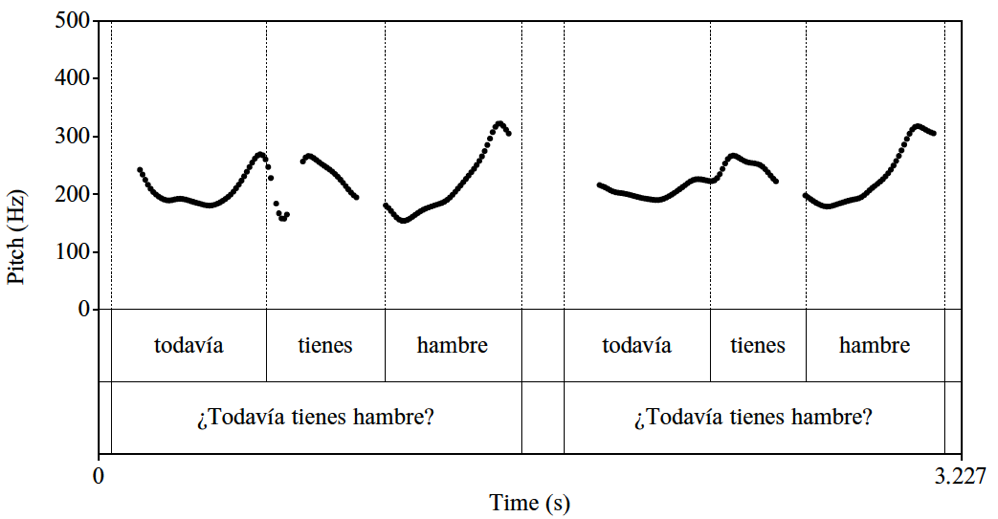
\includegraphics[width=\textwidth]{figures/a03HabilMethodology-img001.png}




\caption{Example of the elicited sentence \textit{¿Todavía tienes hambre?} (‘You’re still hungry?!’) as a semi-spontaneous answer (left) and as a read answer (right), produced by a German female learner of L2 Spanish (Ge\_09\_F).}
\label{fig:3.1}
\end{figure}



Interestingly, many speakers commented that, of the four parts of the experiment, the DCT was the most challenging, but at the same time the most interesting or entertaining task. Recall also that the DCT was recorded at the end of the whole experiment, by which point participants had forgotten that they were being recorded.


\section{Participants}\label{sec:3.2}

Participants were 60 adult L2 learners: 40 L2 Spanish learners (20 L1 Czechs and 20 L1 Germans), and 20 L2 Italian learners with L1 Czech. Besides their L1, the participants were also selected according to their “L2 proficiency level”. Half of them were independent (B) and another half proficient (C) users according to the \textit{Common European Framework of Reference for Languages} (CEFR). Furthermore, six native speakers of Spanish and six of Italian also took part as a control group. The participants received a small fee in compensation for their participation and all gave prior written consent to be recorded. Additionally, participants were asked whether they had been diagnosed with any hearing or speech disorder. There were no problems reported in this respect.



The Czech participants were recruited by the respective Faculties of Arts at Masaryk University in Brno and Charles University in Prague, the \textit{Hispánica} language school in Brno and the \textit{Instituto Cervantes} in Prague, institutions which kindly supported this project and facilitated the search for participants. It was not easy to find willing volunteers who fulfilled the same criteria, and in spite of all efforts the resulting set of participants was not completely balanced in terms of gender nor homogeneous in terms of L1 variety, the length of time spent living abroad and other variables summarized in Tables below. The recruitment and organisation of L1 German participants proved to be much easier, and this group was also more homogeneous than the Czech group. Nearly all of them were students at Osnabrück University, the two exceptions being two students at the University of Hamburg. All of them belonged to the same L1 -- Western North High German -- variety (cf. \sectref{sec:3.2.1}).



Aside from several of the L1 controls, none of the participants had any kind of close relationship with the interviewer. Moreover, they were unaware of the purpose of the study (i.e., L2 intonation), although they knew that the experiment dealt with research on second language speech. It should be noted that adjustments were made during the experimental procedure to accommodate par\-tic\-i\-pant-specific needs or output. For example, when a participant misunderstood a particular DCT situation, the context description was repeated, up to three times. However, when producing utterances, participants often corrected their output too. No participant displayed an insufficient L2 proficiency to warrant the exclusion of his/her data. By contrast, output from one male Czech L2 Spanish learner (Cz\_03) had to be excluded from the study because of his very high-proficiency (native-like) performance and his linguistic background, which was very different from that of the other participants; this derived from the fact that he had been teaching Spanish at a language school for over 10 years and had been married to a Colombian woman, and therefore was in constant contact with Spanish both at home and work.


\subsection{L2 Spanish learners (L1 Czech and L1 German)}\label{sec:3.2.1}\largerpage[2]

All forty L2 Spanish learners (20 L1 Czechs and 20 L1 Germans) were native speakers except for three Germans, who were (early) bilinguals with a Turkish, Russian or Portuguese background. Despite this fact, I included them in the analysis, for the following reasons.



\begin{enumerate}[label={(\arabic*)}]
\item
          They were born and grew up in Germany with L1 German being a dominant language in the sense used, for example, by \citet{Grosjean1982, Grosjean2008} and \citet{Montrul2013}.



\item
          Their L1 German was judged to be that of a German native speaker by ten other German native speakers in an ad hoc perception experiment.



\item
           Their L2 Spanish was judged to be “Spanish with a typical German accent” by five Spanish native speakers living in Germany in another perception experiment. In this perception experiment, the “foreign accent” of ten L2 Spanish learners with L1 German as well as seven L2 learners with other L1s (American English, Czech, Greek, Italian, Portuguese, Russian, Slovak) was rated independently by a set of Spanish native speakers.
\end{enumerate}\largerpage[2]


The tables below (\tabref{tab:3.2}--\ref{tab:3.3a} for Czech learners and \tabref{tab:3.4}--\ref{tab:3.5a} for German learners) give detailed information about the 40 L2 Spanish participants with regard to gender, age, occupation, L1 variety, Spanish proficiency, language experience abroad, age of L2 learning, language use (i.e., active use of Spanish per week at the time of the interview) and knowledge of other foreign languages.

As already noted, one half of the speakers in each group were independent L2 users (B1--B2) and the other half were proficient L2 users (C1--C2). The average age when the participants began to acquire Spanish was roughly the same for the two groups (CZ: 17 years old; GE: 18 years old). The two groups also shared the fact that English had been the L2 they acquired first, with exception of two Czech speakers (Cz\_02, Cz\_18) whose first L2s were German and Russian, respectively. The two areas with greatest differences between the groups were the frequency of active use of Spanish per week at the time of the experiment and the time spent in a Spanish-speaking country. Whereas Czech participants reported using Spanish actively almost eight hours a week on average, German participants did so only two hours a week. This was quite surprising, since all the German participants were students attending university and studying Spanish at the time of the experiment, whereas only ten Czech participants were studying Spanish at university. Concerning the variety of Spanish to which they were exposed, participants reported being exposed to non-native as well as native Spanish-speaking instructors coming from mainland Spain, the Canary Islands or Latin American countries. As already pointed out in \chapref{ch:2}, it would have been very difficult to control for this potentially intervening factor because it would have implied accepting only those participants who had been exposed to one particular Spanish dialect. However, the majority of participants had had more contact with Peninsular Spanish or were currently in contact with it. Finally, it should be noted that the two groups differed in terms of the distribution of occupations, but this was due to the manner of their recruitment, as described above.\pagebreak


\begin{table}[p]
\begin{tabularx}{\textwidth}{lllQQ}

\lsptoprule

{Person} & {Gender} & {Age} & {Occupation} & {L1 variety}

{Bohemian (B)}

{Moravian (M)\footnote{See Czech dialectal map in \figref{fig:3.3}}}\\
\midrule
Cz\_01 & M & 30 & independent & M (Brno; dialect II)\\
Cz\_02 & M & 40 & teacher (German) & M (Prostějov; dialect II)\\
Cz\_04 & F & 29 & artist & M (Vítkov; dialect II)\\
Cz\_05 & F & 29 & shop assistant & M (Brno; dialect II)\\
Cz\_06 & F & 23 & student (Spanish) & B (Prague; dialect Ib)\\
Cz\_07 & F & 21 & student (Spanish) & B (Prague surround.; dialect Ib)\\
Cz\_08 & F & 20 & student (Spanish) & B (Teplice; north-western part of B.)\\
Cz\_09 & F & 24 & nurse & B (Prague; dialect Ib)\\
Cz\_10 & F & 27 & student (translation and interpreting) & B (Prague; dialect Ib)\\
Cz\_11 & F & 19 & student (Spanish) & M (Třebíč; dialect II)\\
Cz\_12 & M & 33 & web designer & B (Prague; dialect Ib)\\
Cz\_13 & F & 31 & administrative assistant & B (Čáslav; dialect Ib)\\
Cz\_14 & M & 22 & student (Spanish) & B (Prague surround.; dialect Ib)\\
Cz\_15 & F & 24 & student (Spanish) & B (Prague surround.; dialect Ib)\\
Cz\_16 & F & 20 & student (Spanish) & B (Prague; dialect Ib)\\
Cz\_17 & M & 20 & student (Spanish) & B (Prague; dialect Ib)\\
Cz\_18 & F & 23 & student (Spanish) & B (Prague; dialect Ib)\\
Cz\_19 & M & 34 & shop assistant & B (Prague; dialect Ib)\\
Cz\_20 & F & 45 & secretary & B (Prague; dialect Ib)\\
Cz\_21 & M & 31 & manager & B (Prague; dialect Ib)\\
\lspbottomrule
\end{tabularx}
\caption{\label{tab:3.2}Gender, age, occupation and L1 variety of L2 Spanish participants (with L1 Czech).}
\end{table}

\begin{table}[p]
\small
\begin{tabularx}{\textwidth}{ll>{\raggedright\arraybackslash}p{.25\textwidth}QQQ}

\lsptoprule

{Person} & {Proficiency} & {Experience in a L2 area} & {Age at onset of acquisition} & {Active Spanish per week} {(hours)} & {Other} {L2s\footnote{The following abbreviations of L2 were used: ARAB (Arabic), CAT (Catalan), CRO (Croatian), DU (Dutch), EN (English), FIN (Finish), FR (French), GE (German), HU (Hungarian), ITA (Italian), LAT (Latin), POL (Polish), POR (Portuguese), RU (Russian), SPA (Spanish), SLO (Slovak), SWE (Swedish), TU (Turkish)}}\\
\midrule
Cz\_01 & C2 & 1 year in different locations in Spain, 1 year in different Latin American countries & 22 & 5 & EN, RU\\
\tablevspace
Cz\_02 & B1 & short visits to different locations in Spain & 35 & 1 & EN, GE, RU\\
\tablevspace
Cz\_04 & B2 & short visits to different locations in Spain & 20 & 2 & EN, GE\\
\tablevspace
Cz\_05 & B1 & short visit in Catalonia & 14 & 2 & EN, CRO\\
\tablevspace
Cz\_06 & C1 & short visits to different locations in Spain, Mexico, Guatemala & 17 & 20 & EN, GE\\
\tablevspace
Cz\_07 & B2 & no stay abroad & 16 & 1--2 & EN, POL\\
\tablevspace
Cz\_08 & B2 & no stay abroad & 15 & 20 & EN, CAT\\
\tablevspace
Cz\_09 & B2 & 1 year in different locations in Spain & 21 & 10 & EN, GE\\
\tablevspace
Cz\_10 & B2 & short visits to different locations in Spain, Mexico & 13 & 10 & EN, ITA, POR\\
\tablevspace
Cz\_11 & C1 & 1 month in the south of Spain & 17 & 8 & EN, FR, GE, POR, LAT, CAT\\
\midrule
\end{tabularx}
\caption{\label{tab:3.3a} Foreign language background of L2 Spanish participants (with L1 Czech).}
\end{table}

\begin{table}[p]\ContinuedFloat
\small
\begin{tabularx}{\textwidth}{ll>{\raggedright\arraybackslash}p{.25\textwidth}QQQ}

\midrule

{Person} & {Proficiency} & {Experience in a L2 area} & {Age at onset of acquisition} & {Active Spanish per week} {(hours)} & {Other} {L2s}\\
\midrule
Cz\_12 & B2 & short visits to different locations in Spain and Central America & 24 & 2 & EN, FR, GE\\
\tablevspace
Cz\_13 & C2 & 5 years in Spain & 16 & 3 & EN, GE, POR, RU\\
\tablevspace
Cz\_14 & C1 & short visits to different locations in Spain & 17 & 2–3 & EN, FR\\
\tablevspace
Cz\_15 & C1 & 6 months in Barcelona and short visits to different locations in Spain & 10 & 3 & EN, CAT\\
\tablevspace
Cz\_16 & C2 & short visits to different locations in Spain & 10 & 40\footnote{At the time of recording, the speaker was exposed to Spanish almost 40 hours a week because of her temporary job in an international company.} & EN\\
\tablevspace
Cz\_17 & C1 & 3 months in Valencia & 13 & 4 & EN\\
\tablevspace
Cz\_18 & C1 & 10 months in Valencia;

short visits to Cuba & 17 & 8 & EN, DU\\
\tablevspace
Cz\_19 & B2 & 1 month in northern Spain & 10 & 2 & EN, FR, ITA\\
\tablevspace
Cz\_20 & B1 & short visits to different locations in Spain & 19 & 1 & EN, FR, RU\\
\tablevspace
Cz\_21 & C1 & 2 years in Barcelona & 14 & 1 & EN\\
\lspbottomrule
\end{tabularx}

%\caption{\label{tab:3.3b} Foreign language background of L2 Spanish participants (with L1 Czech) (continued).}
\end{table}

\begin{table}[p]
\begin{tabularx}{\textwidth}{lllQ>{\raggedright\arraybackslash}p{3.2cm}}

\lsptoprule

{Person} & {Gender} & {Age} & {Occupation} & {L1 variety}

{(West Low German)}\\
\midrule
Ge\_01 & M & 37 & student, teacher (Spanish) & Ibbenbüren\\
Ge\_02 & F & 24 & student (Spanish) & Osnabrück\\
Ge\_03 & M & 26 & student (Spanish) & Osnabrück\\
Ge\_04 & F & 24 & student (Spanish) & Bünde\\
Ge\_05 & F & 20 & student (Spanish) & Lohne\\
Ge\_06 & F & 27 & student (Spanish) & Osnabrück\\
Ge\_07 & F & 28 & student (Spanish) & Hamburg\\
Ge\_08 & F & 27 & student (Spanish) & Hamburg\\
Ge\_09 & M & 21 & student (Spanish) & Osnabrück\\
Ge\_10 & M & 21 & student (Spanish) & Osnabrück\\
Ge\_11 & M & 24 & student (Spanish) & Osnabrück\\
Ge\_12 & F & 24 & student (Spanish) & Osnabrück\\
Ge\_13 & F & 21 & student (Spanish) & Osnabrück\\
Ge\_14 & M & 26 & student (Spanish) & Osnabrück\\
Ge\_15 & F & 23 & student (Spanish) & Osnabrück\\
Ge\_16 & F & 25 & student (Spanish) & Georgsmarienhütte\\
Ge\_17 & F & 22 & student (Spanish) & Osnabrück\\
Ge\_18 & F & 27 & student (Spanish) & Osnabrück\\
Ge\_19 & F & 23 & student (Spanish) & Osnabrück\\
Ge\_20 & F & 25 & student (Spanish) & Münster\\
\lspbottomrule
\end{tabularx}

\caption{\label{tab:3.4}Gender, age, occupation and L1 variety of L2 Spanish participants (with L1 German).}
\end{table}

\begin{table}[p]
\small
\begin{tabularx}{\textwidth}{ll>{\raggedright\arraybackslash}p{.25\textwidth}QQQ}

\lsptoprule

{Person} & {Proficiency} & {Experience in a L2 area} & {Age at onset of acquisition} & {Active}

{Spanish per week} & {Other}

{L2s}\\
\midrule
Ge\_01 & C1 & short visits to different locations in Spain & 32 & 3 & EN\\
\tablevspace
Ge\_02 & C1 & 6 months in Chile & 20 & 4 & EN, FR, ITA\\
\tablevspace
Ge\_03 & B2 & 5 months in Cádiz & 20 & 2 & EN, LAT\\
\tablevspace
Ge\_04 & C2 & 2 years in Lanzarote & 17 & 2 & EN, FR\\
\tablevspace
Ge\_05 & B2 & no stay abroad & 15 & 0.5 & EN, FR\\
\tablevspace
Ge\_06 & C1 & no stay abroad & 17 & 2 & EN, FR\\
\tablevspace
Ge\_07 & C1 & 6 months in Barcelona & 14 & 0 & EN, CAT, FIN, HU, ITA, SWE\\
\tablevspace
Ge\_08 & C1 & 6 months in Alicante & 17 & 0 & EN, FR, POR, RU\\
\tablevspace
Ge\_09 & B1 & short visits to different locations in Spain & 14 & 4 & EN, FR\\
\tablevspace
Ge\_10 & B2 & short visits to different locations in Spain & 13 & 2 & EN, FR\\
\tablevspace
Ge\_11 & B2 & 1 year in Mexico and different places in Spain & 15 & 3 & EN, FR\\
\midrule
\end{tabularx}

\caption{\label{tab:3.5a}Foreign language background of L2 Spanish participants (with L1 German).}
\end{table}

\begin{table}[p]\ContinuedFloat
\small
\begin{tabularx}{\textwidth}{ll>{\raggedright\arraybackslash}p{.25\textwidth}QQQ}

\midrule

{Person} & {Proficiency} & {Experience in a L2 area} & {Age at onset of acquisition} & {Active}

{Spanish per week} & {Other}

{L2s}\\
\midrule
Ge\_12 & C1 & 6 months in Cádiz & 20 & 2 & EN, FR\\
\tablevspace
Ge\_13 & B2 & short visits to different locations in Spain & 16 & 3 & EN, FR\\
\tablevspace
Ge\_14 & C1 & 5 months in Valladolid & 16 & 1 & EN

(2L1 = RU)\\
\tablevspace
Ge\_15 & B2 & 6 months in Costa Rica & 17 & 5 & EN, FR\\
\tablevspace
Ge\_16 & C2 & 9 months in Galicia,

many short visits to different Spanish-speaking countries & 19 & 2 & EN, FR

(2L1 = TU)\\
\tablevspace
Ge\_17 & B2 & 3 months in Andalucía & 16 & 2 & EN, LAT\\
\tablevspace
Ge\_18 & B1 & short visits to different locations in Spain & 23 & 2 & EN, LAT\\
\tablevspace
Ge\_19 & B2 & short visits to different locations in Spain & 21 & 3 & FR, DU, EN (2L1 = POR)\\
\tablevspace
Ge\_20 & C1 & 3 months in Madrid,

6 months in Alicante & 17 & 2 & EN, FR\\
\lspbottomrule
\end{tabularx}

%\caption{\label{tab:3.5b}Foreign language background of L2 Spanish participants (with L1 German) (continued).}
\end{table}\clearpage


With regard to their L1 variety, the German participants constituted a more homogenous group, since they all spoke one main German variety, namely, Western North High German (\figref{fig:3.2}).

\begin{figure}[p]
%%\includegraphics[width=\textwidth]{figures/a03HabilMethodology-img002.tif}
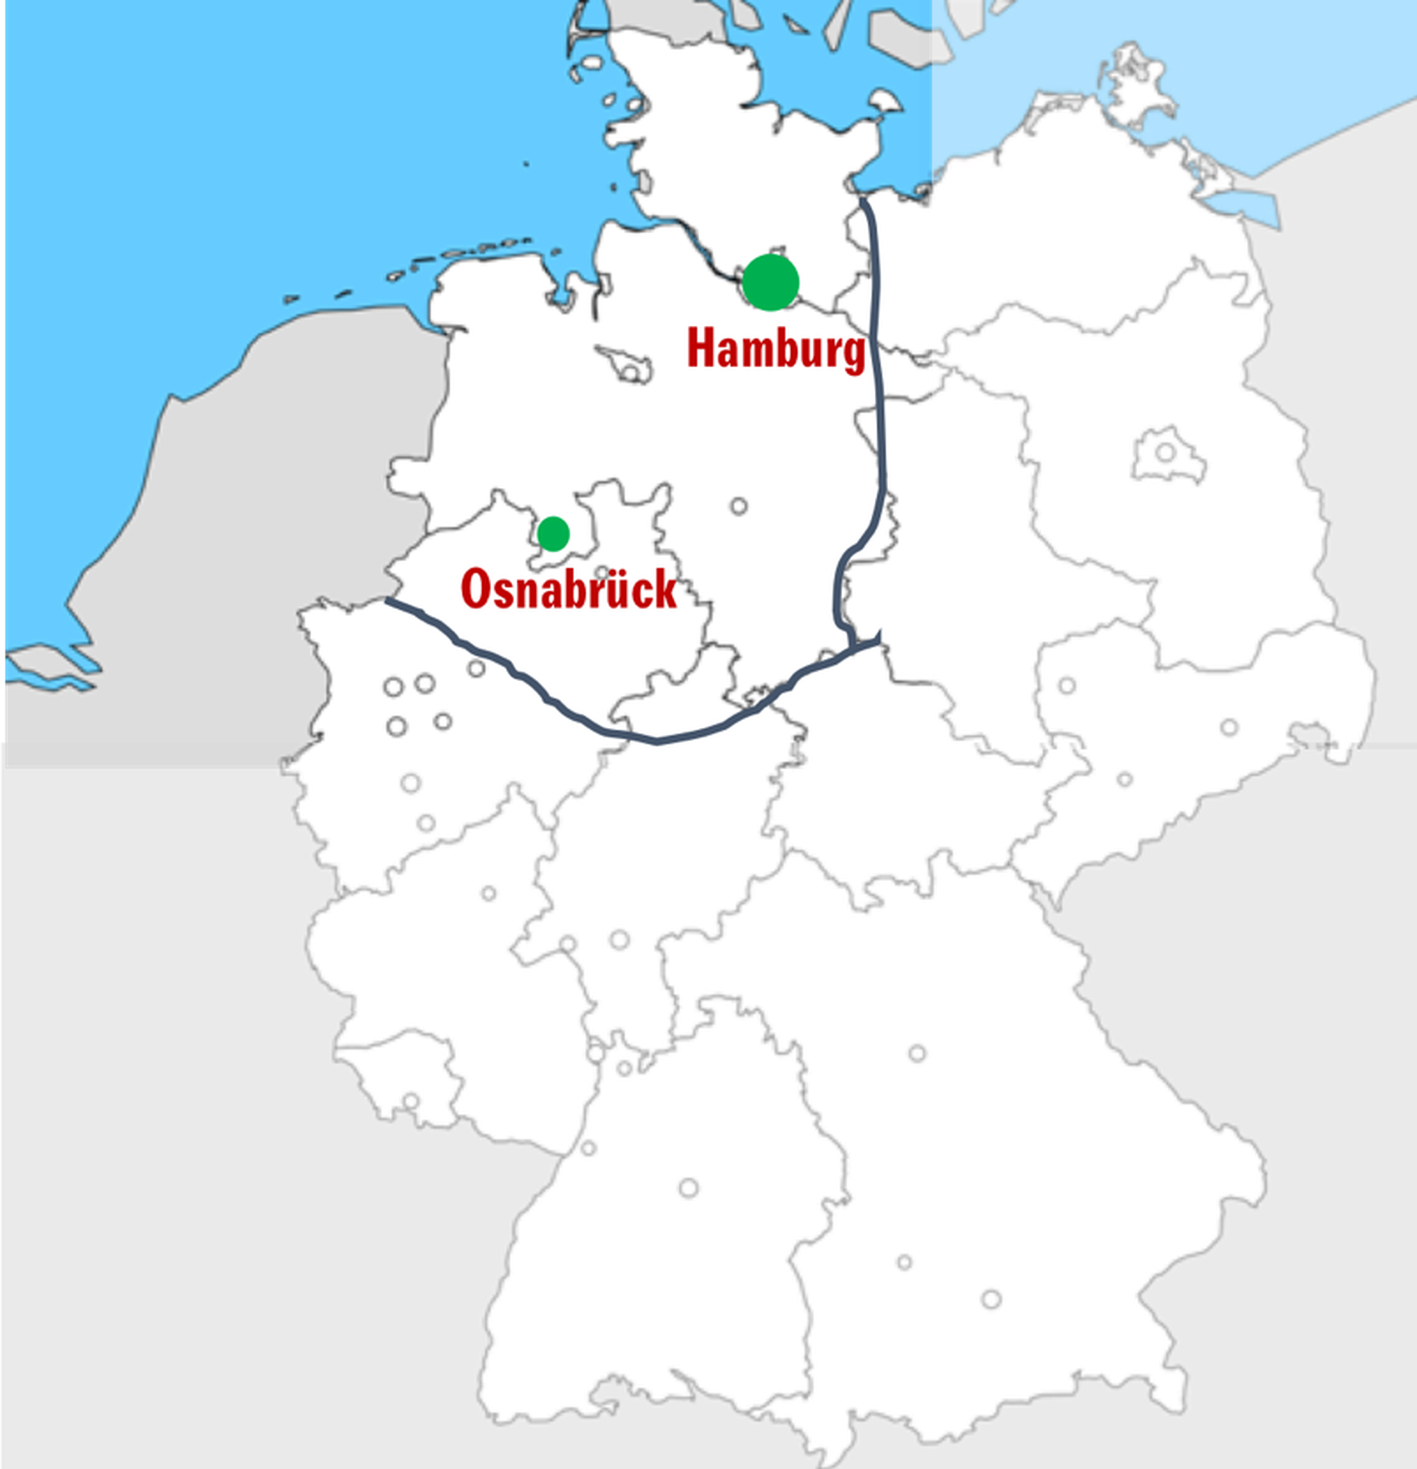
\includegraphics[width=.7\textwidth]{figures/a03HabilMethodology-img002-new.png}
\caption{The geographic distribution of Western North High German (own representation).}
\label{fig:3.2}
\end{figure}



In contrast, the Czech participants came from two main dialectal areas, Bohemian and Moravian (see, e.g., \citealt{Cvrček2010, ŠimáckováEtAl2012}), whose distribution is illustrated in \figref{fig:3.3}. These two dialects of Czech may -- according to the literature -- diverge slightly in intonation, as we noted in \chapref{ch:2} (see \chapref{ch:4}).




\begin{figure}[p]
%%\includegraphics[width=\textwidth]{figures/a03HabilMethodology-img003.tif}
\includegraphics[width=.7\textwidth]{figures/a03HabilMethodology-img003-new.png}
\caption{Czech dialect map according to \citet{Kloferová2017}.\label{fig:3.3}}
\end{figure}



The fact that the Czech participants reflected two dialect groups was the consequence of practical considerations since, as noted above, I was dependent on cooperation with two universities as well as language schools for recruitment. The Bohemian participants came from Central Bohemia (Dialect Ib in \figref{fig:3.3}) and the Moravian speakers from the centre of the region (Dialect II), with the exception of three speakers who were from the region of Dialects Ia and Id. No speaker came from Silesia, the north-eastern part of the Czech Republic (Dialect IV). All this was considered in the results reported later.


\subsection{L2 Italian learners (L1 Czech)}\label{sec:3.2.2}

The recruitment of twenty L1 Czech learners of Italian (at B or C proficiency levels) was even more challenging than finding L2 Spanish speakers. This was due to not just the reasons outlined above but also the fact that Italian is less popular than Spanish as a foreign language in the Czech Republic at the moment. Thus, this group was especially heterogeneous in terms of L1 variety as seen in \tabref{tab:3.6}. Nor was the group at all balanced for gender, with males being grossly underrepresented.


\begin{table}[p]
\small
\begin{tabularx}{\textwidth}{lllQQ}

\lsptoprule

{Person} & {Gender} & {Age} & {Occupation} & {L1 variety}

{Bohemian (B)}

{Moravian (M)}

{Silesian (S)}\\
\midrule
Cz\_31 & F & 24 & student (Italian) & M (Starý Jičín; dialect III)\\
Cz\_32 & F & 38 & linguist & M (Veselí nad Moravou; dialect III)\\
Cz\_33 & F & 26 & student (Italian) & M (Břeclav; dialect III)\\
Cz\_34 & F & 23 & student (Italian) & M (Veselí nad Moravou; dialect III)\\
Cz\_35 & F & 23 & student (Italian) & S (Frýdek-Místek; dialect IVa)\\
Cz\_36 & F & 29 & student (Art history) & B (Hradec Králové; dialect Ia)\\
Cz\_37 & F & 30 & student (Italian) & M (Brno; dialect II)\\
Cz\_38 & F & 37 & travel consultant & M (Brno; dialect II)\\
Cz\_39 & F & 36 & PhD student (Italian literature) & M (Kuřim; dialect II)\\
Cz\_40 & F & 23 & student (Italian) & B (Pelhřimov; dialect Ic)\\
Cz\_41 & F & 26 & student (Italian) & S (Ostrava; dialect IVa)\\
Cz\_42 & F & 22 & student (Italian) & S (Ostrava; dialect IVa)\\
Cz\_43 & F & 24 & student (Italian) & M (Brno; dialect II)\\
Cz\_44 & M & 43 & information technology & B/M (Karlovy Vary, but more than 25 years living in Brno)\\
Cz\_45 & F & 22 & student (Italian) & M (Brno; dialect II)\\
Cz\_46 & M & 28 & student (Italian and general linguistics) & M (Brno; dialect II)\\
Cz\_47 & F & 24 & administration & M (Brno; dialect II)\\
Cz\_48 & F & 26 & student (andragogy) & B (Nové Město nad Metují; dialect Ia)\\
Cz\_49 & F & 27 & administration in international company (IT) & M (Brno; dialect II)\\
Cz\_50 & F & 31 & recruitments (personal agency) & M (Strážnice; dialect III)\\
\lspbottomrule
\end{tabularx}

\caption{\label{tab:3.6}Gender, age, occupation and L1 variety of L2 Italian participants (with L1 Czech).}
\end{table}


The participants also differed largely with regard to time spent living in an L2 area, active exposure to Italian per week and knowledge of other foreign languages (\tabref{tab:3.7a}).


\begin{table}[p]
\small
\begin{tabularx}{\textwidth}{ll>{\raggedright\arraybackslash}p{.25\textwidth}QQQ}

\lsptoprule

{Person} & {Proficiency} & {Experience in a L2 area} & {Age at onset of acquisition} & {Active Italian}

{per week} & {Other}

{L2s}\\
\midrule
Cz\_31 & C1 & 1 month in the Dolomites, 5 months in Siena & 18 & 2 & EN, FR\\
\tablevspace
Cz\_32 & B1 & short trips to different locations in Italy & 20 & 1 & EN, GE, SPA, FR\\
\tablevspace
Cz\_33 & C1 & 5 months in Padua & 19 & 4 & EN, FR\\
\tablevspace
Cz\_34 & B2 & short trips to different locations in Italy & 14 & 2 & EN, FR\\
\tablevspace
Cz\_35 & C1 & 16 months (Roma, Ravenna, Cervia) & 18 & 28 & EN, SPA\\
\tablevspace
Cz\_36 & B2 & three months in Parma, several weeks in Turin and Milan & 20 & 0 & EN, GE\\
\tablevspace
Cz\_37 & C2 & 3 months in Perugia; regular trips for work & 23 & 40 (work) & EN, FR\\
\tablevspace
Cz\_38 & C2 & 5 years in Toscana, Rome & 18 & 0 & EN, GE\\
\tablevspace
Cz\_39 & C2 & 6 years in San Benedetto del Tronto & 19 & 2 & EN, FR, SPA\\
\tablevspace
Cz\_40 & B2 & different short trips to Italy & 18 & 4 & EN, GE, FR\\
\midrule
\end{tabularx}
\caption{\label{tab:3.7a}Foreign language background of L2 Italian participants (with L1 Czech).}
\end{table}

\begin{table}[p]\ContinuedFloat
\small
\begin{tabularx}{\textwidth}{ll>{\raggedright\arraybackslash}p{.25\textwidth}QQQ}

\midrule

{Person} & {Proficiency} & {Experience in a L2 area} & {Age at onset of acquisition} & {Active Italian}

{per week} & {Other}

{L2s}\\
\midrule
Cz\_41 & C1 & 6 months in Rome; many short trips to Ravenna, & 19 & 5 & EN, GE\\
\tablevspace
Cz\_42 & B1 & 2 months in Genoa & 19 & 10 & EN, FR\\
\tablevspace
Cz\_43 & B2 & different short trips to different locations in Italy & 18 & 6 & EN\\
\tablevspace
Cz\_44 & B1 & 2 weeks in Calabria & 33 & 2 & EN, GE, SPA, FR, RU\\
\tablevspace
Cz\_45 & C1 & 4 months in Perugia & 20 & 4 & EN\\
\tablevspace
Cz\_46 & C1 & different short trips to different locations in Italy & 20 & 5-6 & EN, PORT\\
\tablevspace
Cz\_47 & B1 & 5 months in Verona & 20 & 0 & EN\\
\tablevspace
Cz\_48 & B2 & 14 months in Firenze & 11 & 2 & EN, FRA, ARAB\\
\tablevspace
Cz\_49 & C1 & different short trips to different locations in Italy & 12 & daily (Italian boyfriend from Abruzzo & EN, SPA, GE\\
\tablevspace
Cz\_50 & B1 & 3 months in Calabria & 25 & 1 & EN\\
\lspbottomrule
\end{tabularx}

%\caption{\label{tab:3.7b}Foreign language background of L2 Italian participants (with L1 Czech) (continued).}
\end{table}

\subsection{Control groups}\label{sec:3.2.3}

Since the intonation of different Spanish and Italian dialects has already been amply explored in the literature (see, e.g., \citealt{PrietoRoseano2010, GiliFivelaEtAl2015}), only six L1 (European) Spanish native speakers and six L1 Italian native speakers (Northern varieties) carried out the full experiment, the idea being that the data I obtained from these two control groups would serve as a basis for comparison with the experimental L2 learners’ groups and the literature (\tabref{tab:3.8} and \ref{tab:3.9}).


\begin{table}[p]
\begin{tabularx}{\textwidth}{lllQQ}
\lsptoprule
{Person} & {Gender} & {Age} & {Occupation} & {Dialect}\\
\midrule
Sp\_01 & F & 25 & student (Spanish and English) & Central-Southern Castilian\\
Sp\_02 & F & 24 & student (Spanish and German) & Central-Southern Castilian\\
Sp\_03 & F & 30 & university lecturer and researcher & Northern Castilian\\
Sp\_04 & F & 25 & university researcher & Northern Castilian\\
Sp\_05 & F & 38 & Spanish teacher & Central-Southern Castilian\\
Sp\_06 & F & 19 & student (secondary grammar school) & Central-Southern Castilian\\
\lspbottomrule
\end{tabularx}

\caption{\label{tab:3.8}L1 Spanish control group for the study (dialects based on \citealt{Hualde2005}).}
\end{table}

\begin{table}[p]
\begin{tabularx}{\textwidth}{lllQl}
\lsptoprule
{Person} & {Gender} & {Age} & {Occupation} & {Dialect}\\
\midrule
Ita\_01 & M & 20 & student (Italian) & Toscana\\
Ita\_02 & F & 29 & phonetician & Piemonte\\
Ita\_03 & F & 30 & university lecturer and researcher & Veneto\\
Ita\_04 & F & 21 & student (psychology) & Lombardia\\
Ita\_05 & F & 29 & German teacher & Piemonte\\
Ita\_06 & M & 30 & IT & Piemonte\\
\lspbottomrule
\end{tabularx}

\caption{\label{tab:3.9}L1 Italian control group for the study.}
\end{table}\clearpage


A second set of control data was obtained by having the experimental groups -- the Spanish and Italian L2 learners -- perform two of the experimental tasks (reading the chapter from \textit{The Little Prince} and doing the DCT) in their respective native languages. For the purposes of the present study, DCT data from twelve randomly selected L1 Czech and ten L1 German speakers were examined.


\section{Experimental procedure}\label{sec:3.3}

Czech participants carried out the experiment in March and May 2016, March 2017, February 2018 and February 2019 at either the Laboratory of Behavioural and Linguistic Studies \textit{LABELS} at Charles University in Prague, at the \textit{Hispánica} language school in Brno or in a soundproof laboratory at the Masaryk University Faculty of Informatics in Brno. Most of the German participants performed the experiment during the 2016 and 2017 summer and winter semesters at Osnabrück University; for two participants the experiment was run in May 2016 at the University of Hamburg.



In all cases, the experiments were carried out in a quiet location and the data were recorded directly as WAV files by means of a Marantz HD Recorder (PMD 671) and a Sennheiser microphone (ME 64) positioned at a distance of approximately 30\,cm from the speaker’s mouth (sample rate 44,100\,Hz, 16 bit). Subsequent data transcription along with acoustic analysis of all target utterances was performed with version 6.0.26 of the Praat software (\citealt{BoersmaWeenink1992-2019}). The whole experiment was recorded in an open, friendly and rather informal atmosphere in order to minimize tension on the part of participants and to ensure that recorded data were as natural as possible. The experimental materials and all instructions were presented to participants in the form of a PowerPoint presentation, so that direct intervention by the interviewer was limited. The whole experiment was conducted in the target language (Spanish or Italian); we switched into German or Czech only at the end of the experiment, when L1 data were collected. One recording session took around one hour and it was preceded by a general questionnaire soliciting demographic information and contact details of participants and a linguistic background questionnaire collecting information on factors such as age of L2 learning, amount of L2 experience, L2 use per week that can shape the participants’ individual characteristics of pronunciation (cf., \citealt{PiskeEtAl2001}).


\section{Analysis and measurements}\label{sec:3.4}

Although the full study involved the collection of data by means of a production experiment with several tasks, for the purpose of the present study only the data from the last experimental task, the DCT, will be analysed and discussed. While the DCT comprised a total of 25 prompt situations, only 18 situations per L2 learner have been selected for the final analysis offered here (see \chapref{ch:4}, \textit{\nameref{ch:4}}). The resulting corpus subjected to analysis thus consisted of a total of 1080 target items, including broad focus statements, pragmatically marked statements, different types of yes/no questions and wh-questions as well as vocatives. The intonation of imperatives and greetings was left aside for future investigation; exclamatives are treated in \citet{Pešková2022b}. The process yielded a total of 4.717 tonal events for final analysis and interpretation. This number comprises prenuclear pitch accents and nuclear accents with boundary tones. Each audio file was subjected to acoustic analysis by means of Praat software (\citealt{BoersmaWeenink1992-2019}), and orthographic transcription of the audio data as well as ToBI annotation of pitch contours (\sectref{sec:3.4.1}) were added. In order to capture further fine-grained phonetic differences between the learner varieties, F0 change as well as durational cues were measured (\sectref{sec:3.4.2}).


\subsection{Transcription of intonation}\label{sec:3.4.1}\largerpage

As already explained in \chapref{ch:2}, the transcription of F0 is based on two important tonal entities in Spanish and Italian, namely pitch accents (tones associated with tonic syllables) and boundary tones (tones associated with the edges of phrases). To date, the labelling of intonational data has generally been performed manually. Since manual labelling has been criticized for subjectivity and low reliability, I also employed a practical and innovative software tool for automatic transcription of (Spanish) intonation, called \textit{Etiquetador ToBI}, Eti\_ToBI \citep{Elvira-GarcíaEtAl2016}. Most importantly, the Eti\_ToBI transcriber performs a pitch track analysis based on linguistic features, using the Sp-ToBI system implemented in the script. Although the tool is intended to be applied to L1 Spanish data, in fact it works fairly well for Italian data and L2 data too (albeit requiring manual corrections).\footnote{As explained in \chapref{ch:2}, in Italian, there are two pitch accents and two boundary tones, hence four different labels, that are not assumed for Spanish: H*+L, L*+>H, and H!H\%, L!H\% respectively.} This automatic transcriber, running as a Praat script and transcribing up to 50 (simple) sentences per minute, labels all pitch accents and boundary tones. I will briefly explain how the tool works.



Before using Eti\_ToBI, a TextGrid with one interval tier (\textit{Text}) and one point tier (\textit{Break indices}) was created. The first tier, located underneath the spectrogram, obtained a phonetic transcription of the utterance analysed, divided into syllables (stressed syllables have to bear the IPA stress mark in order for Eti\_ToBI to be able to recognize the target tonal event).\footnote{The positions of the syllable boundaries as well as the end of IP-final words in Praat were determined according to several phonetic criteria -- such as formant structure, intensity and pitch periods -- which have been applied in previous studies on rhythm (see, e.g., \citealt{WhiteMattys2007, GrabeLow2002, GabrielKireva2014b}).}



In the second tier, levels of prosodic phrasing were annotated with break indices (BI). The Eti\_ToBI tool differentiates between three of these levels of structuring within the prosodic hierarchy: prosodic words (BI 1), intermediate phrases (ip) (BI 3) and intonational phrases (IP) (BI 4). An example of Eti\_ToBI tonal notation as applied to the Spanish sentence \textit{Se vende la casa bonita} ‘The nice house is for sale’ is given in \REF{ex:3:1}:


\ea\label{ex:3:1} \glllll {\textit{Se}]} {\textit{\textbf{ven}.de}]} {\textit{la}]}    {\textit{\textbf{ca}.sa}]} {\textit{bo.\textbf{ni}.ta}]}.\\
     {\hphantom{Se}\textbar}            {\hphantom{ven.de}\textbar}            {\hphantom{la}\textbar}               {\hphantom{ca.sa}\textbar}                   {\hphantom{bo.ni.ta}\textbar}\\
   {\hphantom{Se}BI 0}         {\hphantom{ven.de}BI 1}        {\hphantom{la}BI 0}           {\hphantom{ca.sa}BI 1}      {\hphantom{bo.ni.ta}BI 4}\\
          {}   (*)    {}   (*)            {(*)  (\%)}\\
\textsc{refl}   sell-\textsc{3ps.sg}    the\textsc{{}-f}     house         nice\textsc{{}-f}\\


\glt ‘The nice house is for sale.’
\z

After all TextGrids with the two corresponding tiers had been prepared, the script was run. As it applies the script, Eti\_ToBI offers the user the possibility of manually correcting the labels it proposes. On the present occasion this feature was particularly useful: First, the program was operating on L2 data, which show different F0 patterns. Second, the script is very sensitive to voiceless consonants (especially fricatives) and distorted some measurements. And finally, certain curve properties and interesting F0 shapes in the L2 data might have been missed had we relied solely on the points predetermined by the tool.


An example of the final output of the script is shown in \figref{fig:3.4}. The usual Praat output (spectrogram, F0 contour and orthographic transcription) is followed by a tier showing BI level numbers and three further tiers providing tonal information.




\begin{figure}
%%\includegraphics[width=\textwidth]{figures/a03HabilMethodology-img004.tif}
\includegraphics[width=\textwidth]{figures/a03HabilMethodology-img004-new.png}



\caption{Eti\_ToBI output for the L2 Spanish utterance \textit{Prefiero mandarinas} ‘I prefer tangerines’, produced by an L1 German participant (Ge\_03\_M).}
\label{fig:3.4}
\end{figure}



The first of these three tonal tiers comprises the \textit{surface} analysis of the utterance and allows tritonal accents (not included in the current ToBI systems).\footnote{In ToBI notation, all phonetically tritonal pitch accents are transformed into phonologically bitonal pitch accents, except for Argentinean “Italianized” Spanish, where the phonological inventory includes a tritonal L+H*+L accent \citep{GabrielEtAl2010}. Since Eti\_ToBI is designed to recognise intonational patterns of the ten dialects of Spanish described in \citet{PrietoRoseano2010}, initially the script offers the user the possibility of choosing whether the tritonal accent of Argentinean Spanish should be reported in one of the phonological tiers or not. This was very useful for the L1 and L2 Italian data.} The transcription of the prenuclear accent is thus a L+H*+H rise in the stressed syllable, which continues to rise in the post-stressed syllable. The smaller F0 movement of this complex tone is indicated between parentheses (in this case, L+(H*+H)). The authors of the Eti\_ToBI tool call this type of transcription a “transliteration of F0” (\citealt[775]{Elvira-GarcíaEtAl2016}) which contains many non-contrastive details similar to what is seen in a narrow phonetic transcription. Here, the Eti\_ToBI tags pitch movements greater than 1.5 semitones and takes into account three parameters: F0 shape, F0 alignment and F0 range. It thus gives detailed information about tonal events. In contrast to the Sp-ToBI conventions, which contain in total 14 labels for all tonal events (seven for pitch accents and seven for boundary tones), the surface transcription in Eti\_ToBI distinguishes between 13 labels for prenuclear pitch accents, 15 for nuclear pitch accents and 10 for boundary tones. Eti\_ToBI thus predicts a total of 150 possible nuclear configurations (all theoretically possible combinations of nuclear tones and boundary tones). The standardized (Spanish) ToBI permits only 61 combinations, though presumably not all combinations are available in the language.\footnote{As already noted in \chapref{ch:2}, the present study assumes a total of nine pitch accents and seven boundary tones. Although the proposed labels lack certain phonetic details, they appeared appropriate in the cross-linguistic comparison undertaken here and suitable for assessing results.}



The second tonal tier offers a \textit{deep} analysis (to use \citegen{Elvira-GarcíaEtAl2016} term), that is, a broad phonetic transcription, in which all tritonal pitch accents are converted into bitonal labels. This transcription was crucial for the present study. And finally, the third tonal tier provides a \textit{standardized} (conventionalized) transcription that “translates” some of the nuclear configurations into the current phonology-based (Spanish) ToBI. In fact, there are only a few small differences between the \textit{deep} and \textit{standardized} levels. For example, the configuration L+<H* H\% is converted into L+H* H\%, because L+<H* does not appear in the nuclear position in Spanish. Hypothetically, if we transform these three levels into the Spanish segmental level, the \textit{surface level} would give us complete information about non-contrastive sounds, the \textit{deep} \textit{level} would present a broad phonetic transcription containing only allophones important for one phonological system, and the \textit{standardized} \textit{level} would provide us with a phonological transcription, as illustrated in \REF{ex:3:2}.


\ea\label{ex:3:2}  Type of transcription

\gllll {\normalfont Orthographic transcription}      {\normalfont<vendido> ‘sold’}\\
{Narrow phonetic transcription}    [bɛ̃n̪ˈdi\textsuperscript{ð}o]\\
{Broad phonetic transcription}      [bɛnˈdiðo]\\
{Phonemic (phonological) transcription}   /benˈdido/\\
\z



What the transcription in \REF{ex:3:2} does not offer is information about formants (resonating frequencies of the vocal tract) F1 and F2, which are important for the acoustic characterization of all vowels (and which can be measured by means of speech software). By the same token, the ToBI transcription does not provide any detailed information on pitch range in F0 values (for example, a pitch accent realized with a rising tone L+H* does not say much about “how far” the L tone is from the H tone); nor does it provide further prosodic information such as the length of the event in ms. Some of these parameters will be measured and reported here separately (see \sectref{sec:3.4.2}).



Given all these considerations, the question arose as to how useful and reliable Eti\_ToBI would be for the purposes of the present study. I therefore ran a pilot experiment in which the program analysed and labelled 690 tonal entities (prenuclear pitch accents and nuclear configurations), and simultaneously I labelled the same materials manually. Though Eti\_ToBI proved unable to measure all instances (due to fricatives or creaky voices), in general agreement between the manual labelling and the Eti\_ToBI output was relatively high at 79\% (\textit{N} = 561). As noted by \citet[6]{Elvira-García2016}, “using Eti\_ToBI not only can speed up phonetician works in order to let them focus more in theory, but it can also highlight fails in the theoretical framework they use.” In other words, the script can correct or point out an erroneous interpretation, since it calculates differences in semitones. Nevertheless, we cannot forget that it is still a program, a bit hypersensitive to acoustic signal (mainly micro-prosody effects, voiceless consonants, fricatives and creaky voices), and the Praat pitch detection algorithm may thus perform inadequately (which can result in a distorted picture of the F0 contour and an erroneous label). Another issue to keep in mind is the effectiveness of Eti\_ToBI when it is run on L2 data. Although the program takes into account three levels of labelling, namely ToBI-standardized labelling (language-specific) and broad and narrow labelling (non-language-specific), it does not recognise the various phenomena that may result from L1 intonation interference. Hence, as noted above, manual correction of the automatic labelling proved to be unavoidable here. Since the present study deals with L2 data, transparent, consistent and especially non-language-specific labels were used for the analysis, which were already presented in Chapter 2. No inter-transcriber reliability of the labelling system of the present study has been assessed so far, but since the pilot study on labelling uniformity with Eti\_ToBI was run and the agreement was relatively high, the proposed labels can be deemed appropriate for the purposes of the study.



In spite of the transparent labels (presented in \chapref{ch:2}), transcription of L2 intonation was not straightforward in all cases and several difficulties were encountered in applying ToBI labels to the data. For example, when a pitch accent displayed a pitch movement that was only slightly rising, it was not clear whether to treat it as a L+H or just a H or L pattern. This was especially the case of “Czech” Spanish, which is characterized by a more flat pitch tracking. Following the Eti\_ToBI annotation parameters, the rising label LH was only assumed when the difference between L and H was larger than 1.5 semitones. Stress displacement represented another problematic issue for labelling, especially in data from several Czech participants (recall that Czech has initial stress). This is illustrated in \figref{fig:3.5}, where a Czech participant starts the sentence \textit{Prefiero mandarinas} from quite a high initial point (labelled as \textit{Hi}) and produces the overall pitch contour without any observable larger pitch movements. Interestingly, as a native Czech speaker myself I perceived Czech accenting on the first syllable, but Spanish native speakers consulted did perceive Spanish accenting (thus on the second syllable) here, perhaps because of additional non-tonal cues such as intensity or because of the access to the meaning. The target pitch accents associated with the stressed syllables (-\textit{fie-}, -\textit{ri-}) showed no slope at all or just a very slight one.




\begin{figure}[p]
%%\includegraphics[width=\textwidth]{figures/a03HabilMethodology-img005.tif}
\includegraphics[width=.9\textwidth]{figures/a03HabilMethodology-img005-new.png}
\caption{Spectrogram and F0 trace for the statement \textit{Prefiero mandarinas} ‘I prefer tangerines’, produced by a L1 Czech learner of Spanish (Cz\_02\_M). It is realized with an initial high tone (Hi), a H+L* prenuclear pitch accent and a !H* L\% nuclear configuration.}
\label{fig:3.5}
\end{figure}

\begin{figure}[p]
%%\includegraphics[width=\textwidth]{figures/a03HabilMethodology-img006.tif}
\includegraphics[width=.9\textwidth]{figures/a03HabilMethodology-img006-new.png}
\caption{Spectrogram and F0 trace for the statement \textit{Prefiero mandarinas} ‘I prefer tangerines’, produced by a Spanish native speaker (Sp\_01\_F). It is realized with a H+L* prenuclear pitch accent and a L+¡H* L\% nuclear configuration.}
\label{fig:3.6}
\end{figure}



The dilemma presented by such data was whether to mark the word on the first syllable \textit{pre-} with H* or on the second syllable -\textit{fie-} as H+L* and to decide which syllable anchored a pitch accent. In general, I opted for the second option (“Spanish” stress placement) because of similar scenarios observed in L1 Spanish native speakers too (\figref{fig:3.6}). In \figref{fig:3.6} the sentence-initial prenuclear position does not show the expected L+<H* rising pattern described in the literature. One possible interpretation of the falling prenuclear pattern (H+L*) with the peak on the first syllable may be that it either indicates deaccenting of the known material or represents a result of secondary stress.\footnote{A secondary stress in Spanish is an optional phenomenon and mostly observed in different forms of public or emphatic speech (\citealt{Hualde2007,Hualde2009, Hualde2010}).} Or it can be simply a case of variation of tonal patterns that is very similar to the variation one measures, for instance, in vowels that very often display a large dispersion and variability.


In some cases, a rising pattern occurs on a syllable other than the “target” syllable and the stress shift was not only visible but also clearly perceived. This is illustrated in \figref{fig:3.7}, where an L1 German learner of Spanish inappropriately places stress on the initial syllable of \textit{todavía} ‘still’ *[ˈto.ða.βi.a] instead of on the penultimate syllable [to.ða.ˈβi.a]. Other instances will be reported individually in \chapref{ch:4}.




\begin{figure}
%%\includegraphics[width=\textwidth]{figures/a03HabilMethodology-img007.tif}
\includegraphics[width=\textwidth]{figures/a03HabilMethodology-img007-new.png}



\caption{Spectrogram and F0 trace for the yes/no question \textit{¿Todavía tienes hambre?} ‘Are you still hungry!?’, produced by an L1 German learner of Spanish (Ge\_03\_M).}
\label{fig:3.7}
\end{figure}


It should also be added that the tonal analysis of the L2 data (i.e., the application of ToBI labelling) was conducted in two directions and a total of four steps: (1) one sentence type per all speakers, (2) all sentences per one speaker, (3) step 2 was repeated after one month and, finally, (4) step 2 was repeated after six months again. Only about 4\% of all tonal events were modified again in the final labelling session.



Finally, besides the tonal annotation of pitch contours, the present study includes two additional parameters that are not integrated into the ToBI systems but which serve to capture further fine-grained phonetic differences between the learner varieties and the Spanish and Italian control groups. These parameters include (1) the pitch change for each tonal event, and (2) the duration of the whole sentences (measurements of duration cues concerning words and syllables will be left for future).


\subsection{Pitch change of tonal events and duration cues}\label{sec:3.4.2}

\begin{sloppypar}
Regarding the measurements of the pitch change, I marked the lowest and highest F0 points of every tonal event using the Praat command “Move cursor to minimum/maximum pitch”. As a rule, only voiced segments were measured and all F0 points were checked and corrected manually or removed from the results, if necessary. Not all F0 contours produced by speakers were ideal for pitch measurements due to devoicing, the presence of voiceless consonants or creaky voice. In those instances where the F0 was reduced due to creaky voice, the value obtained by the script was doubled \citep{ArvanitiEtAl2017} or repaired by the Praat MAUSMOOTH script (“MAnually and AUtomatically SMOOTHed”; \citealt{Cangemi2015}), which permits the user to make manual corrections of extracted contours and obtain repaired values.
\end{sloppypar}


Figures \ref{fig:3.8}--\ref{fig:3.9} and \ref{fig:3.10}--\ref{fig:3.11} illustrate measurements of F0 points in one statement and one yes/no question in L2 Spanish as produced by a Czech learner and a German learner, respectively. In order to examine the pitch change of the tonal events, the lowest and the highest points of these features were extracted by means of the following calculations:\pagebreak


\begin{itemize}
\item F0\textsubscript{1} $-$ F0\textsubscript{2} = first prenuclear pitch accent (PA1)
\item F0\textsubscript{3} $-$ F0\textsubscript{4} = second (mostly medial) prenuclear pitch accent (PA2)
\item F0\textsubscript{5} $-$ F0\textsubscript{6} = nuclear pitch accent (NA)
\item F0\textsubscript{6} $-$ F0\textsubscript{F} = boundary tone (BT), final F0 (F0\textsubscript{F})
\end{itemize}


\begin{figure}[p]
\includegraphics[width=\textwidth]{figures/a03HabilMethodology-img008.pdf}
\caption{Example of the F0 points analysed. Spectrogram and F0 trace for the statement \textit{Marisa come mandarinas} ‘Marisa eats tangerines’ (L1 Czech participant; Cz\_02\_M).}
\label{fig:3.8}
\end{figure}



\begin{figure}[p]
\includegraphics[width=\textwidth]{figures/a03HabilMethodology-img009.pdf}
\caption{Example of the F0 points analysed. Spectrogram and F0 trace for the yes/no question \textit{¿Vamos a tomar una cerveza?} ‘Shall we go have a beer?’ (L1 Czech participant; Cz\_02\_M).}
\label{fig:3.9}
\end{figure}


\begin{figure}[p]
%%\includegraphics[width=\textwidth]{figures/a03HabilMethodology-img010.emf}
\includegraphics[width=\textwidth]{figures/a03HabilMethodology-img010.pdf}

\caption{Example of the F0 points analysed. Spectrogram and F0 trace for the statement \textit{Marisa come mandarinas} ‘Marisa eats tangerines’ (L1 German participant; Ge\_03\_M).}
\label{fig:3.10}
\end{figure}

\begin{figure}[p]
%%\includegraphics[width=\textwidth]{figures/a03HabilMethodology-img011.emf}
\includegraphics[width=\textwidth]{figures/a03HabilMethodology-img011.pdf}

\caption{Example of the F0 points analysed. Spectrogram and F0 trace for the yes/no question \textit{¿Vamos a tomar una cerveza?} ‘Shall we go have a beer?’ (L1 German participant; Ge\_03\_M).}
\label{fig:3.11}
\end{figure}


In a final step, I calculated a pitch change for each tonal event, by expressing ratios between F0 minimum vs. F0 maximum first. A pitch change refers here to a fixed ratio of frequencies if we understand a measurement as “the estimation of the ratio of some magnitude of a quantitative attribute to a unit of the same attribute” \citep[358]{Michell1997}. Magnitudes, such as maximal and minimal F0 within a tonal event, “stand in relations (\textit{ratios}) to one another and can be expressed as real numbers” \citep[356]{Michell1997}. The advantage of the ratio scale is that it has a non-arbitrary zero value. This is important because speech shows a range of variation and differences between speakers. For example, women have in general a wider F0-range in Hz than men. With ratios, the between-sex (or other speakers’ idiosyncratic) differences disappear. Let us imagine the two following scenarios: In speaker A, the min F0 point of the initial prenuclear accent has a value of 100\,Hz and the max F0 point 200\,Hz; in speaker B, the min. F0 point has a value of 300\,Hz and the max F0 point 400\,Hz. In both cases, the pitch change is 100\,Hz, but the ratios between the two F0 points are different, 1:2 in speaker A and 3:4 in speaker B, respectively. This means that the F0 max point has 50\% of the pitch change (increase) in speaker A, but only 25\% in speaker B; this was calculated as follows:

\begin{description}
\item [Speaker A:]   F0 max $-$ F0 min = 200\,Hz $-$ 100\,Hz / 200 * 100 = 50\%
\item [Speaker B:]   F0 max $-$ F0 min = 400\,Hz $-$ 300\,Hz / 400 * 100 = 25\%
\end{description}


And finally, I measured and compared the duration of the whole sentences. It is well known that speech rate can be a secondary prosodic characteristic of different types of sentences (see, e.g., \citealt{vanHeuvenvanZanten2005} regarding the speech rate of polarity questions in different languages). Since some disparities between the languages under study were observed, it was presumed that the learner groups might also differ from natives with respect to durational cues in L2 Spanish or Italian.


\chapter{L2 Spanish and L2 Italian intonation patterns}\label{ch:4}

The main objective of this chapter is to present the intonational patterns in L2 Spanish and L2 Italian, which are based on the phonetic level of labelling, and to answer the following general question: \textit{Are tonal events (prenuclear pitch accents, nuclear pitch accents, boundary tones) produced in a target-like manner or are they characterized by transferred features from the learners’ L1?} If the first scenario is true, then German and Czech learners of L2 Spanish should become closer in their production of the target language and the two Czech groups (L2 Spanish vs. L2 Italian) should perform differently from each other. If the second scenario is true, there should be no or very little difference between the two L1 Czech groups and larger differences between the two L2 Spanish learner groups. A third scenario offers the possibility that both target-like and L1-like patterns together with mixed patterns will be found. Here a further question arises, namely, \textit{Which tonal events and sentence types cause learners the most difficulties and why?}



In the subsequent chapter, I will summarize the overall picture of the interlanguage varieties (\sectref{sec:5.1}), then discuss the main results in terms of accuracy (\sectref{sec:5.2}) and within \citegen{Mennen2015} L2 Intonation Learning theory (LILt) (\sectref{sec:5.3}), before addressing the role of proficiency in explaining variation in L2 data (\sectref{sec:5.4}). It should be mentioned here in advance that the factor \textit{L1} but not the factor \textit{Proficiency} was shown to have a statistically important effect on L2 intonation deviations. Possible reasons behind this finding will also be discussed in \chapref{ch:5}.



The present chapter is organised in five sections according to the type of sentence collected by means of an intonation questionnaire: neutral statements (\sectref{sec:4.1}), non-neutral statements (\sectref{sec:4.2}), yes/no questions (\sectref{sec:4.3}), wh-questions (\sectref{sec:4.4}) and vocatives (\sectref{sec:4.5}). The tonal analysis is supported by examples from the learners’ and controls’ productions. In order to facilitate comprehension of the data, each section follows a common structure and covers the following issues:

\begin{enumerate}[label=(\arabic*)]
\item  Presentation and comparison of intonational properties of L1 languages (Spanish, Italian, German, Czech) regarding the respective sentence type; and formulation of underlying hypotheses and/or research questions that are derived from the main features.
\item  Presentation and comparison of tonal events (prenuclear pitch accents, nuclear pitch accents, boundary tones) between the L2 Spanish varieties, as produced by L1 German and L1 Czech speakers.
\item  Presentation and comparison of tonal events (prenuclear pitch accents, nuclear pitch accents, boundary tones) between L2 Spanish and L2 Italian, both produced by L1 Czech learners.
\item  Presentation and comparison of other prosodic cues (pitch change, durational cues) between L2 and L1 Romance varieties.
\item  Interpretation and summary of the most important findings and verification of the postulated hypotheses.
\end{enumerate}

\section{Neutral statements}\label{sec:4.1} %4.1 /
\subsection{Neutral statements in L1 Spanish, L1 Italian, L1 German and L1 Czech}\label{sec:4.1.1}

In all the languages under study, neutral broad-focus statements have a kind of “toboggan”-shaped contour (in \citeauthor{Sosa1999}'s \citeyear{Sosa1999} term), starting with a rise or high tone in prenuclear position and ending in a fall. Such a decline in F0 over the course of the statement is common in many intonational languages. However, the languages may differ in two ways: in the type of prenuclear pitch accent and in the realization of the nuclear configuration. By means of the production experiment (see \textit{Methodology}, \chapref{ch:3}), we obtained two neutral declarative sentences per speaker, which were set in a neutral context (\ref{ex:4:1}--\ref{ex:4:2}).\footnote{The prompt contexts for \REF{ex:4:1} and \REF{ex:4:2} were as follows:

\begin{exe}
\exr{ex:4:1} They ask you what fruit you prefer. You say that you prefer tangerines. (What fruit do you prefer?)
\exr{ex:4:2} Look at the picture and tell me what is happening here.
\end{exe}}

\ea\label{ex:4:1} \glll {\normalfont Italian}     \textit{Preferisco i mandarini.} \\
Spanish   \textit{Prefiero mandarinas.} \\
{}      {‘I prefer tangerines.’}\\


\ex\label{ex:4:2} \glll  {\normalfont Italian}     \textit{Marisa mangia dei mandarini.} \\
Spanish   \textit{Marisa come mandarinas.} \\
{}      {‘Marisa is eating tangerines.’}\\
\z

Declaratives across Italian varieties typically have rising prenuclear pitch accents with the peak aligned within the stressed syllable (L+H*) followed mostly by a H+L* L\% nuclear configuration (\citealt{GiliFivelaEtAl2015}). In contrast, (Peninsular) Spanish declaratives are characterized by rising prenuclear pitch accents with a delayed peak (L+<H*) and a low nuclear accent (L*) followed by a low boundary tone (L\%) (see, e.g., \citealt{Face2003, PrietoRoseano2010, HualdePrieto2015}, among many others). The falling contour in Spanish declaratives begins already at the end of the penultimate prosodic word, from which point the pitch continues descending.


Figures \ref{fig:4.1}--\ref{fig:4.2} and Figures \ref{fig:4.3}--\ref{fig:4.4} exemplify the prototypical intonation of this sentence type, first in L1 Italian, and then in L1 Spanish; the target sentences have one or two prenuclear accents.


Now I will present broad focus statements in the first languages of the learners. According to the literature (see, e.g., \citealt{Uhmann1991, Féry1993, GriceBaumann2002, GriceEtAl2005a, PetroneNiebuhr2014}), German declaratives are characterized by monotonal or bitonal prenuclear pitch accents. The most typical accent in \citegen{Féry1993} terminology is the \textit{topic-accent}, which is phonetically realized as a rising tone on the stressed syllable (Féry uses the label L*+H). \citet{GriceBaumann2002} as well as \citet{PetroneNiebuhr2014} report that prenuclear accents typically have a high tone with an optional smooth rise in the preceding pretonic syllable (they use the label H*). If the rise is located within the stressed syllable, the authors propose L+H*, which will be adopted here. The nuclear configuration of the statements typically has a H+L* nuclear accent (\figref{fig:4.5}) or a \textit{focus-type} L+H* tone (\figref{fig:4.6}) followed by a final low tone (L\%). \citet[82]{Féry1993} claims that L1 speakers of German “perceive the falling realization on the nuclear accent as the most natural one in declarative sentences.”\largerpage

The situation is slightly different in Czech, which has phonological accentual phrases /L* Ha/, consisting of a pitch accent and a boundary tone, and defined as rhythmic units with a (mostly) rising pitch from one stressed syllable to the next (\citealt{PeškováEtAl2018}, see also \sectref{sec:2.3.2.1}). (We could transcribe the L*+Ha sequences phonetically with a delayed peak, that is, as L+<H* or with a L*+H pitch accent). There are two main ways to realize prenuclear positions in broad-focus statements in Czech: either L* Ha is found in both initial and medial positions (\figref{fig:4.7}) or an initial L* Ha is followed by a medial H* Ha pattern (i.e., a high plateau) (\figref{fig:4.8}).{\interfootnotelinepenalty=10000\footnote{In \citet{PeškováForthcoming} I report inter-speaker variation in Czech declarative sentences. Some speakers realize the sentences with a high plateau in the initial position, from which the tone falls steadily until the end. However, intra-speaker variation is very low, meaning that each speaker has his/her own preferences and remains relatively consistent in the production of different sentence types.}}


\begin{figure}[p]
\includegraphics[width=\textwidth]{figures/Figure_4.1.png}
\caption{Waveform, spectrogram and F0 trace of the statement \textit{Preferisco i mandarini} (‘I prefer tangerines’) in L1 Italian \mbox{(F\_2)} produced with H+L* L\%.}
\label{fig:4.1}
\end{figure}

\begin{figure}[p]
\includegraphics[width=\textwidth]{figures/Figure_4.2.png}
\caption{Waveform, spectrogram and F0 trace of the statement \textit{Marisa mangia dei mandarini} (‘Marisa is eating tangerines’) in L1 Italian \mbox{(F\_2)} produced with H+L* L\%.}
\label{fig:4.2}
\end{figure}

\begin{figure}[p]
\includegraphics[width=\textwidth]{figures/Figure_4.3.png}
\caption{Waveform, spectrogram and F0 trace of the statement \textit{Prefiero mandarinas} (‘I prefer tangerines’) in L1 Spanish \mbox{(F\_5)} produced with L* L\%.}
\label{fig:4.3}
\end{figure}

\begin{figure}[p]
\includegraphics[width=\textwidth]{figures/Figure_4.4.png}
\caption{Waveform, spectrogram and F0 trace of the statement \textit{Marisa come mandarinas} (‘Marisa is eating tangerines’) in L1 Spanish \mbox{(F\_11)} produced with L* L\%.}
\label{fig:4.4}
\end{figure}

\begin{figure}
\includegraphics[width=\textwidth]{figures/Figure_4.5.png}
\caption{Waveform, spectrogram and F0 trace of the statement \textit{Ich mag Mandarinen} (‘I like tangerines’) in L1 German \mbox{(F\_05)} produced with H+L* L\%.}
\label{fig:4.5}
\end{figure}

\begin{figure}
\includegraphics[width=\textwidth]{figures/Figure_4.6.png}
\caption{Waveform, spectrogram and F0 trace of the statement \textit{Marisa isst Mandarinen} (‘Marisa is eating tangerines’) in L1 German \mbox{(F\_16)} produced with L+H* L\%.}
\label{fig:4.6}
\end{figure}

\begin{figure}
\includegraphics[width=\textwidth]{figures/Figure_4.7.png}
\caption{Waveform, spectrogram and F0 trace of the statement \textit{Marisa jí mandarinky} (‘Marisa is eating tangerines’) in L1 Czech \mbox{(M\_21)} produced with H* L\%.}
\label{fig:4.7}
\end{figure}

\begin{figure}
\includegraphics[width=\textwidth]{figures/Figure_4.8.png}
\caption{Waveform, spectrogram and F0 trace of the statement \textit{Marisa jí mandarinky} (‘Marisa is eating tangerines’) in L1 Czech \mbox{(F\_34)} produced with L* L\%.}
\label{fig:4.8}
\end{figure}

The behaviour of the control participants was consistent with this dual pattern, since they realized the nuclear pitch accent either with a high tone (H*) as in \figref{fig:4.7} or with a gradual fall from the last Ha (L*) as in \figref{fig:4.8}. The final low boundary L\% closes the sentence; but very exceptionally, the statement can also end in (!)H\%. This holds true especially for young speakers and spontaneous speech. To the best of my knowledge, this aspect has not been analysed and interpreted in any study thus far, but in \citet{PeškováForthcoming} I report such isolated cases in L1 Czech (see \figref{fig:4.9}). Why and in which contexts speakers do so is still an open question.

\begin{figure}
\includegraphics[width=\textwidth]{figures/Figure_4.9.png}
\caption{Waveform, spectrogram and F0 trace of the statement \textit{Eva maluje mandarinky} (‘Eva draws tangerines’) in L1 Czech produced with L* !H\% (from \citealt{PeškováForthcoming}).}
\label{fig:4.9}
\end{figure}


\tabref{tab:4.1} summarizes the inventory of nuclear accents and boundary tones for declaratives in L1 Spanish, Italian, German and Czech.


\begin{table}
\begin{tabular}{lll}
\lsptoprule
Boundary tones\slash & \\
Nuclear accents & {L\%} & {(!)H\%}\\\midrule
{H+L*} & Italian, German & \\
{L*} & Spanish, Czech & (Czech)\textsuperscript{exception}\\
{L+H*} & German\footnote{The L+H* L\% nuclear configuration is typical for narrow focus in German. I introduce this pattern in \tabref{tab:4.1}, because the controls produced it very frequently in the given contexts.} & \\
{H*} & Czech & \\
\lspbottomrule
\end{tabular}
\caption{Summary of the most characteristic declarative patterns in Italian, Spanish, German and Czech.}
\label{tab:4.1}
\end{table}

Based on the cross-linguistic differences stated above, the four following hypotheses were posed:

\begin{enumerate}[label=H\arabic*,font=\PeskovaColonAfterItem]
\item\label{neutral-h1}
 Since /L* Ha/ in Czech is phonetically similar to L+<H* in Spanish, we can expect that Czech learners of Spanish will have an advantage in the realization of the target prenuclear pitch accents (i.e., positive transfer will occur). In contrast, German learners of Spanish will tend to realize prenuclear pitch accents with L+H*.

\item\label{neutral-h2}
 Given that L1 German speakers tend to realize the nuclear pitch accent with a rise (L+H*), we can expect negative transfer from L1 German to L2 Spanish.

\item\label{neutral-h3}
 Working on the assumption that the learners not only transfer their L1 features but are also capable of acquiring new categories, we can expect that “Czech” declaratives in L2 Italian will contrast with “Czech” declaratives in L2 Spanish. This is predictable because the two Romance languages differ in the alignment of rising prenuclear pitch accents (L+H* vs. L+<H*) and the realization of nuclear tones (H+L* vs. L*).

\item\label{neutral-h4}
 Given that Czech declaratives can also end in a (!)H\%, we can expect to see this pattern in L2 data too (albeit sporadically).

\end{enumerate}

\subsection{Neutral statements in L2 Spanish as produced by L1 Czech and L1 German learners}\label{sec:4.1.2}

The results reveal that L1 Czech and L1 German learners of Spanish differ in the realization of pitch accents. In the initial position (\tabref{tab:4.2}), Czech speakers preferred a standard Spanish pattern L+<H*, that is, a rising tone from the onset of the stressed syllable with a peak located on the posttonic syllable (45\%). In contrast, German learners favoured the L*+H variant of rising tone (57.5\%): the rise starts later on the stressed syllable or on the posttonic syllable. Interestingly, L*+H is assumed to be the typical prenuclear pitch accent in yes/no questions in German (see \sectref{sec:4.3}). The frequency of L+H* in “German” L2 Spanish was lower than expected (only 22.5\%). Perhaps the learners perceive the target L+<H* pattern relatively well but attempt to reproduce it with L*+H (in both cases the peak is in the posttonic syllable). Here controlled perception-production tasks would be useful to better understand this relationship. Moreover, Czech learners realized the first pitch accent also with a falling pattern (H+L*), which is typical especially in isolated Czech words (we will see some examples later). This realization was not found in German learners at all. We can thus say that the observed differences in alignment may be -- at least partly -- due to transfer from the learners’ L1s.\footnote{Pearson’s chi-square and Fisher’s exact tests were run to test relationships between categorical variables and to determine whether there were significant differences between the expected frequencies and the observed frequencies in them. Note also that besides the reported differences in frequency of each tonal pattern, I also report the global proportional difference -- the rightmost column. Furthermore, I provide exact $p$ values, considering 0.05 as a threshold for statistical significance. If a $p$ value is from 0.01 to 0.05, the result is significant, if a $p$ value is from 0.001 to 0.01, it is very significant, and if a $p$ value is less than 0.001, it is highly significant. In all other cases, the result is not significant (n.s.).}

\begin{table}
\begin{tabularx}{\textwidth}{lYYY}

\lsptoprule

{Initial prenuclear pitch accents} & {Czech L2 Spanish} & {German L2 Spanish} & {Difference}\\
\midrule
H* &  2.5\% &  2.5\% &  0.0\%\\
H+L* &  20.0\% &  0.0\% &  20.0\%\\
L*+H &  25.0\% &  57.5\% &  32.5\%\\
L+<H* &  45.0\% &  17.5\% &  27.5\%\\
L+H* &  7.5\% &  22.5\% &  15.0\%\\
\midrule
Total (\textit{n}) & {\itshape 40} & {\itshape 40} &  \PeskovaMean{19.0\%}\\
\multicolumn{4}{r}{$\chi^2(4) = 15.92, p = 0.003$}\\
\lspbottomrule
\end{tabularx}

\caption{Realization of initial prenuclear pitch accents in L2 Spanish declaratives. All values are rounded to the nearest half. For example, 10.3 is rounded down to 10; 10.70 is rounded up to 11; but 10.5 remains unchanged.}
\label{tab:4.2}
\end{table}

It\largerpage{} should be added that five speakers (three Germans, two Czechs) used a high intermediate boundary tone (H-) after the subject \textit{Marisa} in the second sentence, which does not reveal any crucial difference between the groups, however. The intermediate boundary tone after the subject is also common in L1 Spanish (see, e.g., \citealt{FrotaEtAl2007}). Where we find differences again is in the realization of prenuclear accents in the medial position. These accents, which are linked to the verb in the second sentence (\textit{Marisa \textbf{come} mandarinas\slash Marisa \textbf{mangia} dei mandarini}), were realized very differently in comparison to the initial prenuclear pitch accents in both learner varieties (\tabref{tab:4.3}). As we can see, the main pattern in “Czech” L2 Spanish was a sustained high tone extended over the whole verb (H*) (67.5\%); while German learners used predominantly a falling H+L* tone in this position (80\%).

\begin{table}
\begin{tabularx}{\textwidth}{lYYY}

\lsptoprule

{Medial prenuclear pitch accents} & {Czech L2 Spanish} & {German L2 Spanish} & {Difference}\\
\midrule
H* &  67.5\% &  15.0\% &  52.5\%\\
H+L* &  22.5\% &  80.0\% &  57.5\%\\
L+<H* &  10.0\% &  0.0\% &  10.0\%\\
L*+H &  0.0\% & 5.0\% &  5.0\%\\
\midrule
Total (\textit{n}) & {\itshape 20} & {\itshape 20} &  \PeskovaMean{31.25\%}\\
\multicolumn{4}{r}{$\chi^2(3) = 17.32, p = 0.001$}\\
\lspbottomrule
\end{tabularx}

\caption{Realization of medial prenuclear pitch accents in L2 Spanish declaratives.}
\label{tab:4.3}
\end{table}

I assume that the medial tones are the least salient tonal events of the whole contour and that the choice of their type can be linked to the realization of the pitch accent in the nuclear position that follows (\tabref{tab:4.4}): L* or H+L* in the “Czech” variety of Spanish (75\%), and L+H* in the “German” one (65\%).\footnote{Throughout this chapter results will be reported not for nuclear configurations but rather separately for nuclear accents and boundary tones. This is because the number of all possible combinations of tonal events would be too high and complex. However, whenever it seems relevant, the results for the nuclear configuration will be given.}\largerpage{}

\begin{table}
\begin{tabularx}{\textwidth}{Qrrr}

\lsptoprule

{Nuclear accents} & {Czech L2 Spanish} & {German L2 Spanish} & {Difference}\\
\midrule
L* &  50.0\% &  20.0\% &  30.0\%\\
L+H* &  17.5\% &  65.0\% &  47.5\%\\
H* &  7.5\% &  0.0\% & 7.5\%\\
H+L* &  25.0\% &  15.0\% &  10.0\%\\
\midrule
Total (\textit{n}) & {\itshape 40} & {\itshape 40} &  \PeskovaMean{23.75\%}\\
\multicolumn{4}{r}{$\chi^2(3) = 20.08, p = 0.000$}\\
\lspbottomrule
\end{tabularx}

\caption{Realization of nuclear accents in L2 Spanish declaratives.}
\label{tab:4.4}
\end{table}

Interestingly, the L+H* corresponds to the realization of narrow focus in both Spanish and German, and German learners showed a preference for highlighting the nuclear accent, even when the sentences lacked narrow focus. This suggests negative transfer from the L1.


Regarding boundary tones, (almost) all right edges in the L2 Spanish declaratives were realized with a low boundary tone (L\%) (\tabref{tab:4.5}).


\begin{table}
\begin{tabularx}{\textwidth}{Qlll}

\lsptoprule

{Boundary tones} & {Czech L2 Spanish} & {German L2 Spanish} & {Difference}\\
\midrule
L\% &  92.5\% &  100.0\% &  7.5\%\\
(!)H\% &  7.5\% &  0.0\% & 7.5\%\\
\midrule
Total (\textit{n}) & {\itshape 40} & {\itshape 40} &  \PeskovaMean{7.5\%}\\
\multicolumn{4}{r}{$\chi^2(2) = 3.12, p = 0.210$}\\
\lspbottomrule
\end{tabularx}

\caption{Realization of boundary tones in L2 Spanish declaratives.}
\label{tab:4.5}
\end{table}

Only three Czech learners (two intermediate and one advanced) chose a high pattern ((!)H\%) here. One speaker (F\_4) produced the sentence with a soft rise (!H\%) after L*, like the second speaker (F\_9), who did so after a L+H* nuclear accent. The third speaker (F\_13), the advanced one, realized the boundary tone with a very sharp and long rise (H\%) (\figref{fig:4.10}).\footnote{All L2 data were transcribed phonetically in accordance with the pronunciation produced by learners. With regard to vowels, formant frequencies were not measured for the purposes of the present study and thus only symbols [a e i o u] were applied here.} In this example you can also see the realization of the H+L* in the prenuclear position: the high tone is located on the pretonic syllable \textit{pre-}, from which point the tone gradually decreases (the fall is shortly interrupted by the fricative). This falling pattern in the initial position has been commonly observed in L1 Czech declaratives as well, especially short ones.

\begin{figure}


%%\includegraphics[width=\textwidth]{figures/a04HabilResults-img010.tif}
%\includegraphics[width=\textwidth]{figures/a04HabilResults-img010-new.png}
\includegraphics[width=\textwidth]{figures/Figure_4.10.png}


\caption{Waveform, spectrogram and F0 trace of the statement \textit{Prefiero mandarinas} (‘I prefer tangerines’) in L2 Spanish (L1 Czech, F\_13, level C) produced with L* H\%.}
\label{fig:4.10}
\end{figure}

The first interpretation of this finding that comes to mind is that the learners simply made performance errors, seeking the hearer’s confirmation by means of raised pitch as if saying “Is it right? Did I do it well?” (see also \citealt[200]{VanrellEtAl2018} for possible negative effects of intonation questionnaires). Another explanation might be that the (!)H\% is transferred from L1 Czech. The fact that (!)H\% did not occur in the data from German learners would support a transfer hypothesis. Later we will see that two cases of H\% were found in L2 Italian statements, produced by Czech learners too.

\begin{sloppypar}
Figures \ref{fig:4.11}--\ref{fig:4.14} exemplify differences observed between the two learner varieties. The first two sentences (Figures \ref{fig:4.11}--\ref{fig:4.12}) were realized by two German learners. In both cases, we see L+H* L\% nuclear configurations and L*+H prenuclear pitch accents.
\end{sloppypar}



Regarding the Czech variety of L2 Spanish, I selected two sentences with L+<H* prenuclear pitch accents. In the first one the utterance ends with a L* L\% nuclear configuration (\figref{fig:4.13}), while in the second one it is realized with a H* tone in the medial position followed by a H+L* L\% nuclear configuration (\figref{fig:4.14}).

If we compare the last example with the L1 Czech contour in \figref{fig:4.7}, we will notice that both contours are phonetically very similar. This clearly confirms the presence of cross-linguistic influence. Notice that the last word has the same pitch course in L1 Czech and L2 Spanish, as shown in \REF{ex:4:3}.


\ea\label{ex:4:3}
\glll  {\normalfont L1 Czech =} \textit{\textbf{man}–da–rin–ky}         {\normalfont L2 Spanish =} \textit{man–da–\textbf{ri}–nas}\\
          {}     {H\hphantom{*an-d}H\hphantom{-}HL\hphantom{-k}L}         {}    {H\hphantom{an-d}H\hphantom{-}HL\hphantom{-n}L}\\
          {}     {H*\hphantom{an-dH-HL-k}L\%}        {}           {\hphantom{man-da-}H+L* L\%}\\
\z

In concluding this section, I should point out that the Czech data show much more variation and individual differences. For example, one speaker produced both declarative sentences with a high tone at the beginning of the utterance and a steadily falling pattern until the final boundary: H* (or H+L*) H+L* L\% (Figures \ref{fig:4.15}--\ref{fig:4.16}).

\begin{figure}
\includegraphics[width=\textwidth]{figures/Figure_4.11.png}
\caption{Waveform, spectrogram and F0 trace of the statement \textit{Prefiero mandarinas} (‘I prefer tangerines’) in L2 Spanish (L1 German, \mbox{F\_20}, level C) produced with L+H* L\%.}
\label{fig:4.11}
\end{figure}

\begin{figure}
\includegraphics[width=\textwidth]{figures/Figure_4.12.png}
\caption{Waveform, spectrogram and F0 trace of the statement \textit{Marisa come mandarinas} (‘Marisa is eating tangerines’) in L2 Spanish (L1 German, \mbox{F\_08}, level C) produced with L+¡H* L\%.}
\label{fig:4.12}
\end{figure}

\begin{figure}
\includegraphics[width=\textwidth]{figures/Figure_4.13.png}
\caption{Waveform, spectrogram and F0 trace of the declarative statement \textit{Prefiero mandarinas} (‘I prefer tangerines’) in L2 Spanish (L1 Czech, \mbox{M\_01}, level C) produced with L* L\%.}
\label{fig:4.13}
\end{figure}

\begin{figure}
\includegraphics[width=\textwidth]{figures/Figure_4.14.png}
\caption{Waveform, spectrogram and F0 trace of the declarative statement \textit{Marisa come mandarinas} (‘Marisa is eating tangerines’) in L2 Spanish (L1 Czech, \mbox{F\_04}, level B) produced with H+L* L\%.}
\label{fig:4.14}
\end{figure}

\begin{figure}
\includegraphics[width=\textwidth]{figures/Figure_4.15.png}
\caption{Waveform, spectrogram and F0 trace of the statement \textit{Prefiero mandarinas} (‘I prefer tangerines’) in L2 Spanish (L1 Czech, \mbox{F\_20}, level B) produced with H+L* L\%.}
\label{fig:4.15}
\end{figure}

\begin{figure}
\includegraphics[width=\textwidth]{figures/Figure_4.16.png}
\caption{Waveform, spectrogram and F0 trace of the statement \textit{Marisa come mandarinas} (‘Marisa is eating tangerines’) in L2 Spanish (L1 Czech, \mbox{F\_20}, level B) produced with H+L* L\%.}
\label{fig:4.16}
\end{figure}

Both sentences are intonational “copies” of the sentences produced by the same speaker \mbox{(F\_20)} in L1 Czech, shown in \figref{fig:4.17}.

\begin{figure}
\includegraphics[width=\textwidth]{figures/Figure_4.17.png}
\caption{Waveform, spectrogram and F0 trace of the statement \textit{Marisa jí mandarinky} (‘Marisa is eating tangerines’) in L1 Czech \mbox{(F\_20)} produced with L* L\%.}
\label{fig:4.17}
\end{figure}

\subsection{Neutral statements in L2 Italian and L2 Spanish as produced by L1 Czech learners}\label{sec:4.1.3}

At first sight, Czech learners of L2 Italian do not differ from Czech learners of L2 Spanish in the realization of initial prenuclear pitch accents: both groups realize H* or H+L* in 22.5\% of cases and rising prenuclear pitch accents in the majority of cases (77.5\%) (\tabref{tab:4.6}). What is most striking here is the difference in the type of rise: whereas the “Spanish” group prefers a delayed peak (L+<H*) (45\%), the “Italian” group favours a L*+H variant (32.5\%). Interestingly, the L2 learners of Italian realize L+H* in 25\% of cases and thus more closely resemble the target pattern (recall that this pitch accent is the default pattern of prenuclear accents in Italian).

\begin{table}
\begin{tabularx}{\textwidth}{lYYY}

\lsptoprule

{Initial prenuclear pitch accents} & {Czech L2 Spanish} & {Czech L2 Italian} & {Difference}\\
\midrule
H* &  2.5\% &  5.0\% &  2.5\%\\
H+L* &  20.0\% &  17.5\% &  2.5\%\\
L*+H &  25.0\% &  32.5\% &  7.5\%\\
L+<H* &  45.0\% &  20.0\% &  25.0\%\\
L+H* &  7.5\% &  25.0\% &  17.5\%\\
\midrule
Total (\textit{n}) & {\itshape 40} & {\itshape 40} &  \PeskovaMean{11.0\%}\\
\multicolumn{4}{r}{$\chi^2(4) = 8.01, p=0.091$}\\
\lspbottomrule
\end{tabularx}

\caption{Realization of initial prenuclear pitch accents in L2 Spanish and L2 Italian declaratives produced by L1 Czech learners.}
\label{tab:4.6}
\end{table}

Regarding medial prenuclear pitch accents, here too highly significant differences were found (\tabref{tab:4.7}). In 90\% of cases, Czech learners of Spanish produced them with H* or H+L* contours. In contrast, Czech learners of Italian did so only 30\% of the time and, again, preferred different rising pitch accents (L+<H*, L*+H, L+H*).

\begin{table}
\begin{tabularx}{\textwidth}{lYYY}

\lsptoprule

{Medial prenuclear pitch accents} & {Czech L2 Spanish} & {Czech L2 Italian} & {Difference}\\
\midrule
H* &  67.5\% &  10.0\% &  57.5\%\\
H+L* &  22.5\% &  20.0\% &  2.5\%\\
L+<H* &  10.0\% &  30.0\% &  20.0\%\\
L*+H &  0.0\% & 15.0\% &  15.0\%\\
L+H* &  0.0\% & 25.0\% &  25.0\%\\
\midrule
Total (\textit{n}) & {\itshape 20} & {\itshape 20} &  \PeskovaMean{24.0\%}\\
\multicolumn{4}{r}{$\chi^2(5) = 22.33, p = 0.000$}\\
\lspbottomrule
\end{tabularx}

\caption{Realization of medial prenuclear pitch accents in L2 Spanish and L2 Italian declaratives produced by L1 Czech learners.}
\label{tab:4.7}
\end{table}

I assume that these differences are linked to the different realizations of nuclear pitch accents (\tabref{tab:4.8}). In contrast to the L2 Spanish group, the L2 Italian learners clearly prefer a target-like H+L* tone, which is implemented as a fall from a preceding high target. In one case, the learner realized the nuclear accent with a tritonal rise-fall pattern (L+H*+L), also found in narrow (contrastive) focus statements (see \sectref{sec:4.2}). On the other hand, there were no important differences detected in the realization of boundary tones (\tabref{tab:4.9}). It is interesting to see that the learners also produced a (!)H\% boundary tone in two cases.

\begin{table}
\begin{tabularx}{\textwidth}{Qrrr}

\lsptoprule

{Nuclear accents} & {Czech L2 Spanish} & {Czech L2 Italian} & {Difference}\\
\midrule
L* &  50.0\% &  42.5\% &  7.5\%\\
L+H* &  17.5\% &  0.0\% & 17.5\%\\
H* &  7.5\% &  2.5\% &  5.0\%\\
H+L* &  25.0\% &  52.5\% &  27.5\%\\
L+H*+L &  0.0\% & 2.5\% &  2.5\%\\
\midrule
Total (\textit{n}) & {\itshape 40} & {\itshape 40} &  \PeskovaMean{12.0\%}\\
\multicolumn{4}{r}{$\chi^2(4) = 13.15, p = 0.011$}\\
\lspbottomrule
\end{tabularx}

\caption{Realization of nuclear accents in L2 Spanish and L2 Italian declaratives produced by L1 Czech learners.}
\label{tab:4.8}
\end{table}

\begin{table}
\begin{tabularx}{\textwidth}{Qrrr}

\lsptoprule

{Boundary tones} & {Czech L2 Spanish} & {Czech L2 Italian} & {Difference}\\
\midrule
L\% &  92.5\% &  95.0\% &  2.5\%\\
(!)H\% &  7.5\% &  5.0\% &  2.5\%\\
\midrule
Total (\textit{n}) & {\itshape 40} & {\itshape 40} &  \PeskovaMean{2.5\%}\\
\multicolumn{4}{r}{$\chi^2(2) = 1.20, p = 0.541$}\\
\lspbottomrule
\end{tabularx}

\caption{Realization of boundary tones in L2 Spanish and L2 Italian declaratives produced by L1 Czech learners.}
\label{tab:4.9}
\end{table}

Figures~\ref{fig:4.18}--\ref{fig:4.19} illustrate selected sentences in L2 Italian with the realizations highlighted above. In both cases, the nuclear configuration is produced with the target-like pattern H+L* L\%, while prenuclear pitch accents show L*+H or L+H* patterns.

\begin{figure}


%%\includegraphics[width=\textwidth]{figures/a04HabilResults-img018.tif}
%\includegraphics[width=\textwidth]{figures/a04HabilResults-img018-new.png}
\includegraphics[width=\textwidth]{figures/Figure_4.18.png}


\caption{Waveform, spectrogram and F0 trace of the statement \textit{Preferisco i mandarini} (‘I prefer tangerines’) in L2 Italian (L1 Czech, \mbox{F\_34}, level B) produced with H+L* L\%.}
\label{fig:4.18}
\end{figure}

\begin{figure}


%%\includegraphics[width=\textwidth]{figures/a04HabilResults-img019.tif}
%\includegraphics[width=\textwidth]{figures/a04HabilResults-img019-new.png}
\includegraphics[width=\textwidth]{figures/Figure_4.19.png}

\caption{Waveform, spectrogram and F0 trace of the statement \textit{Marisa mangia dei mandarini} (‘Marisa is eating tangerines’) in L2 Italian (L1 Czech, \mbox{F\_43}, level B) produced with H+L* L\%.}
\label{fig:4.19}
\end{figure}

\subsection{L1 vs. L2 neutral statements and further prosodic cues}\label{sec:4.1.4}

In this section (and also in \sectref{sec:4.2.4}, \sectref{sec:4.3.4}., \sectref{sec:4.4.4}, \sectref{sec:4.5.4}), additional prosodic differences or similarities in terms of pitch change and duration will be reported on the basis of general trends. These summarize the overall differences between L1 and L2 varieties and give an idea of how the varieties might sound differently on the whole.


In neutral statements, pitch accents had approximately the same values in prenuclear initial position; interestingly, “Czech” L2 Italian learners showed a slightly higher pitch change than “Czech” L2 Spanish learners (\figref{fig:4.20}). That also applies  for prenuclear medial position, in which only L1 Italian diverges from the other varieties (\figref{fig:4.21}).\footnote{Median prenuclear initial accents: “Czech” Italian 18.11 ratios vs. L1 Italian 15.91 ratios; “Czech” Spanish 14.77 ratios, “German” Spanish 14.70 ratios vs. L1 Spanish 15.46 ratios. Median prenuclear medial accents: “Czech” Italian 6.47 ratios vs. L1 Italian 20.05 ratios; “Czech” Spanish 6.47 ratios, “German” Spanish 8.78 ratios vs. L1 Spanish 9.45 ratios.}


\begin{figure}[p]
%\includegraphics[width=\textwidth]{figures/a04HabilResults-img020.png}
\includegraphics[width=\textwidth]{figures/Figure_20.pdf}
\caption{Pitch change of prenuclear initial pitch accents (ratios) in L2 and L1 varieties (neutral statements).}
\label{fig:4.20}
\end{figure}

\begin{figure}[p]
%\includegraphics[width=\textwidth]{figures/a04HabilResults-img021.png}
\includegraphics[width=\textwidth]{figures/Figure_21.pdf}
\caption{Pitch change of prenuclear medial pitch accents (ratios) in L2 and L1 varieties (neutral statements).}
\label{fig:4.21}
\end{figure}

Larger differences in pitch change showed up also in nuclear accents (\figref{fig:4.22}) across the Italian and Spanish varieties, but not in boundary tones (\figref{fig:4.23}). The larger pitch change in German L2 Spanish complies with the realization of nuclear pitch accents (L+H*) in this variety.\footnote{Median nuclear accents: “Czech” Italian 7.04 ratios vs. L1 Italian 14.46 ratios; “Czech” Spanish 4.79 ratios, “German” Spanish 9.52 ratios vs. L1 Spanish 2.66 ratios. Median boundary tones: “Czech” Italian 6.83 ratios vs. L1 Italian 4.77 ratios; “Czech” Spanish 6.83 ratios, “German” Spanish 8.77 ratios vs. L1 Spanish 6.32 ratios.}


This preliminary result indicates that L2 learners seem to have -- at least to a certain degree -- difficulty reproducing the pitch range of the target language(s). For example, Czech learners of Italian show a much smaller nuclear fall (H+L*), when compared with L1 controls.


\begin{figure}


%\includegraphics[width=\textwidth]{figures/a04HabilResults-img022.png}
\includegraphics[width=\textwidth]{figures/Figure_22.pdf}



\caption{Pitch change of nuclear pitch accents (ratios) in L2 and L1 varieties (neutral statements).}
\label{fig:4.22}
\end{figure}

\begin{figure}


%\includegraphics[width=\textwidth]{figures/a04HabilResults-img023.png}
\includegraphics[width=\textwidth]{figures/Figure_23.pdf}



\caption{Pitch change of boundary tones (ratios) in L2 and L1 varieties (neutral statements).}
\label{fig:4.23}
\end{figure}


At the end of this section, it is worth mentioning differences in speech rate (of the whole sentences) between the learner varieties and the controls. As for Spanish, declarative sentences in learner varieties were produced slightly slower in comparison to L1 Spanish (median: “Czech”  Spanish 1340\,ms, “German” Spanish 1375\,ms vs. L1 Spanish 1307\,ms). This is not surprising, since a slower rate is typical for L2 learners when compared with natives (see, e.g., \citealt{DerwingMunro1997, DerwingEtAl2004}). However, we found an opposite trend in Italian, where durational cues are important: L2 Italian declaratives were produced faster than declaratives in native Italian (median: “Czech” Italian 1478\,ms vs. L1 Italian 1565\,ms). Czech learners of Italian did not accurately produce the duration of the last word with nuclear stress in the utterance (but here a further and more in-depth analysis is still needed). An exemplary analysis of the sentence (\textit{Marisa mangia dei mandarini}) showed clear differences between Czech learners and Italian L1 speakers, in that the latter group realized the word \textit{mandaRIni} -- in proportion to the duration of the sentence -- longer than the learners (43\% vs. 38\%). This preliminary result reveals that L2 learners will also need to take the lengthening properties of the target language into account.


\subsection{Interpretation and summary}\label{sec:4.1.5}

Overall, the results exhibit differences as well as similarities between the two learner varieties of L2 Spanish with different L1 backgrounds as well as between the two learner varieties of two L2s with the same L1 background. This doesn't only support the transfer hypothesis, but rather also points to successful acquisition or at least attempts to produce target-like patterns. The results show where the groups of learners have greater or lesser difficulties. As predicted in the first hypothesis (\ref{neutral-h1}), Czech learners of Spanish performed better than German learners in the realization of L+<H* prenuclear pitch accents (45\% vs. 17.5\%). German learners of Spanish showed greater difficulty in the acquisition of alignment, since they realized prenuclear pitch accents with L+H* (22.5\%) or with a L*+H pattern (57.5\%). This is very interesting as L*+H represents prenuclear pitch accents in yes/no questions in German. Given the fact that German learners do not have L+<H* in their L1 tonal inventory, they might produce a pattern which they know, namely L*+H, which is close to L+<H* (the peak is associated with the posttonic syllable in both cases).


Moreover, Czech learners of Spanish realized initial pitch accents quite frequently with a falling H+L* tone (20\%). We detected this pattern -- with almost the same frequency (17.5\%) -- in “Czech” L2 Italian too. I assume that this type of F0 contours resembles L1 features.



With regard to the second CLI hypothesis (\ref{neutral-h2}), many German learners realized nuclear pitch accents with L+H* in L2 Spanish, as expected given their behaviour in the L1. Likewise, the third hypothesis (\ref{neutral-h3}) that “Czech” declaratives in L2 Italian would differ from the “Czech” declaratives in L2 Spanish was verified: the two L2 Romance varieties differed in the realization of nuclear tones (H+L* vs. L*) as well as in the realization of the initial prenuclear pitch accents. However, the L+H* tone was not found in L2 Italian as frequently as we might have expected; it was attested in only 25\% of the cases.



As to the fourth CLI hypothesis (\ref{neutral-h4}), some Czech learners produced sporadically the neutral declaratives with a (!)H\% boundary tone (7.5\% in L2 Spanish and 5\% in L2 Italian).



What was interesting was the difference observed in the realization of medial pitch accents. Although the set of data was relatively small, the learners seem to have major difficulties approximating target-patterns in this position. The default patterns (L+H* in Italian and L+<H* in Spanish) were only seldom found in the two L2 varieties (25\% vs. 10\%, respectively). I conjecture that medial accents are prosodically less salient than initial pitch accents and especially nuclear configurations, which are traditionally defined as the main carrier of meaning. CLI also plays a role here.


At the end of this section, I would like to make a brief comment on whether the learners achieved a target-like realization of word prominence or made mistakes in stressing the correct syllable in the learner varieties. My very general impression is that both Czech and German learners performed very well regarding the location of the stress (in all sentence types). However, I must also admit that the detection of stress displacement was somewhat tricky. Only when a word obtained “prominence” such as a rising tone on a syllable that was not the target syllable was it easy to tag it as an error (see also \chapref{ch:3}, \sectref{sec:3.4.1}). In other cases, the identification of “stress errors” was not so unequivocal, especially in productions by the Czech learners. As already noted, lexical stress in Czech is a very puzzling phenomenon. Whereas pitch and duration are important for distinguishing stressed from unstressed syllables in Italian, Spanish and German words, there is no such correlate in Czech. Interestingly, as a native Czech speaker I perceived certain words in learners’ L2 productions with “Czech” initial stress, whereas Spanish native speakers consulted in that regard perceived Spanish accenting and Italian native speakers perceived Italian accenting. Presumably this is either because they focused on duration or intensity as a cue for lexical stress or because they had access to the meaning and the learners did not use any crucial cue for lexical stress at all. It is thus of major importance to carry out perception as well as production experiments, ideally with nonsense words and words of differing syllable lengths in order to gain insight into this complex phenomenon and to examine whether there is any kind of (a)symmetry between perception and production of lexical stress.

\section{Non-neutral statements}\label{sec:4.2}
\subsection{Non-neutral statements in L1 Spanish, L1 Italian, L1 German and L1 Czech}\label{sec:4.2.1}
\begin{sloppypar}
The objective of this section is to examine how L2 learners produced marked declarative sentences, in which additional pragmatic meanings are involved. Three of the contexts presented in the intonation task were intended to prompt the production of the following three non-neutral statements: one statement with contrastive focus on the object \REF{ex:4:4} and two statements of the obvious (\ref{ex:4:5}--\ref{ex:4:6}) (see \citealt{Pešková2022b} for further types of non-neutral sentence).\footnote{The prompt contexts for \REF{ex:4:4}, \REF{ex:4:5}, \REF{ex:4:6} were as follows:
\begin{exe}
\exr{ex:4:4} You enter a store where the saleswoman is a little hard of hearing. You tell her that you would like a kilo of oranges, but she doesn’t hear you well and asks you if you want lemons. Tell her that you want oranges.
\exr{ex:4:5} You are with a friend and you explain to him/her that Mary, a mutual friend of yours, is getting married. Your friend asks you who she is marrying. You're surprised that s/he doesn’t know, because everyone knows that Mary is planning to marry her long-time boyfriend, Manuel. Tell him/her that she’s getting married to Manuel.
\exr{ex:4:6} You show a picture of a very famous actor to your friend. S/he asks you who it is. This surprises you, because everybody knows him. How do you react?
\end{exe}}
\end{sloppypar}


\ea\label{ex:4:4} \glll {\normalfont Italian}    \textit{No, arance.}\\
    Spanish   \textit{No, naranjas.}\\
    {}  {‘No, oranges.’}\\

\ex\label{ex:4:5} \glll  {\normalfont Italian}    \textit{Con Manuele!}\\
Spanish   \textit{¡Con Manuel!}\\
  {}    {‘To Manuel (obviously)!’}\\

\ex\label{ex:4:6} \glll  {\normalfont Italian}    \textit{È John Travolta!}\\
Spanish   \textit{¡Es John Travolta!}\\
{}      {‘It’s John Travolta (obviously)!’}\\
\z

First, I will describe the tonal properties of the non-neutral declaratives (\ref{ex:4:4}--\ref{ex:4:6}) in the L1 varieties, based on previous studies as well as the control data collected here.


As we will see, (Peninsular) Spanish differs from the other three languages in the realization of boundary tones. Whereas statements with contrastive focus typically end in a low boundary tone (L\%), statements of the obvious display a complex L!H\% boundary tone. The nuclear accent L+H*, a typical \textit{focus}{}-accent observed in many Spanish varieties (see \citealt{PrietoRoseano2010}), is present in both cases. The control data of the present study match with findings reported in the literature (see \citealt{Estebas-VilaplanaPrieto2010, HualdePrieto2015}). Nuclear configurations in statements of the obvious can also include L+(¡)H* L\%, which was found only in the second statement of the obvious (\textit{¡Es John Travolta!}). Why none of the native speakers used the \textit{obvious}{} boundary tone L!H\% in the second case is not very clear, because the contexts were presented in a very similar manner. The reason behind the different realization might be linked to sentence length, which was one vs. three lexical words, respectively.\footnote{Upon evaluation of the present data and on the basis of this result, two native Spanish speakers were asked to respond to the context of the \textit{Manuel} sentence, but this time formulating a complete sentence \textit{¡María se casa con Manuel!} (‘María is marrying Manuel’) instead of \textit{¡Con Manuel!}. Interestingly, the output was not realized with L!H\% but was more similar to the \textit{Travolta}{} sentence (L* HL\%, L+H* L\%, L+H* HL\%). This phrase-length-related alternation and tonal “flexibility” supports findings and melodic constructs reported in \citet{TorreiraGrice2018}.}  Instead, we obtained two further nuclear configuration patterns in the \textit{Travolta}{} sentence: L* HL\% and L+H* HL\%. The first one, L* HL\%, has been reported as a typical contour for narrow focus or contradiction statements in different varieties of Spanish (see \citealt{Estebas-VilaplanaPrieto2010}), but it seems that it may involve other meanings, as the present data demonstrate. The second pattern, L+H* HL\%, has been reported only in vocatives or pragmatically marked questions, but the present data clearly reveal that it exists in marked declaratives too. Figures \ref{fig:4.24}--\ref{fig:4.26} exemplify the principal contours of marked declaratives in L1 Spanish.


\begin{figure}


%%\includegraphics[width=\textwidth]{figures/a04HabilResults-img024.tif}
%\includegraphics[width=\textwidth]{figures/a04HabilResults-img024-new.png}
\includegraphics[width=\textwidth]{figures/Figure_4.24.png}


\caption{Waveform, spectrogram and F0 trace of the contrastive focus statement \textit{¡No, naranjas!} (‘No, oranges!’) in L1 Spanish \mbox{(F\_12)} produced with L+H* L\%.}
\label{fig:4.24}
\end{figure}

\begin{figure}


%%\includegraphics[width=\textwidth]{figures/a04HabilResults-img025.tif}
%\includegraphics[width=\textwidth]{figures/a04HabilResults-img025-new.png}
\includegraphics[width=\textwidth]{figures/Figure_4.25.png}


\caption{Waveform, spectrogram and F0 trace of the statement of the obvious \textit{¡Con Manuel!} (‘To Manuel!’) in L1 Spanish \mbox{(F\_06)} produced with L+H* L!H\%.}
\label{fig:4.25}
\end{figure}

\begin{figure}


%%\includegraphics[width=\textwidth]{figures/a04HabilResults-img026.tif}
%\includegraphics[width=\textwidth]{figures/a04HabilResults-img026-new.png}
\includegraphics[width=\textwidth]{figures/Figure_4.26.png}


\caption{Waveform, spectrogram and F0 trace of the statement of the obvious \textit{¡Es John Travolta!} (‘It is John Travolta!’) in L1 Spanish \mbox{(F\_11)} produced with L+H* HL\%.}
\label{fig:4.26}
\end{figure}

We do not find such a tonal discrepancy in L1 Italian, where all the sentence types examined were produced systematically with the same nuclear configuration: L+H*+L L\%. As already mentioned, the label L+H*+L is not assumed in Standard Italian ToBI, in which other phonology-based labels are proposed (H*+L, L+H* or L*+>H) (see \citealt{GiliFivelaEtAl2015} for further discussion including dialectal variation). In \sectref{sec:2.2.3}, I argued for the phonetic differentiation between the different patterns, with the L+H*+L nuclear pitch accent phonetically realized as a rise and a fall located within the stressed syllable. The L+H*+L pitch accent can also be implemented as H*+L (the high peak is aligned with the left edge of the stressed syllable) or as H+L* (the high peak is located on the pretonic syllable). Figures \ref{fig:4.27}--\ref{fig:4.29} exemplify the typical contours found in L1 Italian marked declaratives.

\begin{figure}


%%\includegraphics[width=\textwidth]{figures/a04HabilResults-img027.tif}
%\includegraphics[width=\textwidth]{figures/a04HabilResults-img027-new.png}
\includegraphics[width=\textwidth]{figures/Figure_4.27.png}


\caption{Waveform, spectrogram and F0 trace of the contrastive focus statement \textit{No, arance!} (‘No, oranges!’) in L1 Italian \mbox{(F\_06)} produced with L+H*+L L\%.}
\label{fig:4.27}
\end{figure}

Now I will examine the tonal patterns of the marked statements in the L1s of the learners. Like in L1 Italian, the sentences in L1 German are predominantly characterized with a single nuclear configuration, L+(¡)H* L\% (the upstep is not obligatory); in the case of the second sentence (\textit{Manuel!}), L* or L*+H accent types followed by a HL\% boundary tone were also found (Figures \ref{fig:4.30}--\ref{fig:4.32}).\pagebreak

\begin{figure}
\includegraphics[width=\textwidth]{figures/Figure_4.28.png}
\caption{Waveform, spectrogram and F0 trace of the statement of the obvious \textit{Con Manuele!} (‘To Manuel!’) in L1 Italian \mbox{(F\_04)} produced with L+H*+L L\%.}
\label{fig:4.28}
\end{figure}

\begin{figure}
\includegraphics[width=\textwidth]{figures/Figure_4.29.png}
\caption{Waveform, spectrogram and F0 trace of the statement of the obvious \textit{(Ma come!) È John Travolta!} (‘(What?) It’s John Travolta!’) in L1 Italian \mbox{(F\_05)} produced with L+H*+L L\%.}
\label{fig:4.29}
\end{figure}

\begin{figure}
\includegraphics[width=\textwidth]{figures/Figure_4.30.png}
\caption{Waveform, spectrogram and F0 trace of the contrastive focus statement \textit{Nein, Orangen!} (‘No, oranges!’) in L1 German \mbox{(F\_16)} produced with L+¡H* L\%.}
\label{fig:4.30}
\end{figure}

\begin{figure}
\includegraphics[width=\textwidth]{figures/Figure_4.31.png}
\caption{Waveform, spectrogram and F0 trace of the statement of the obvious \textit{Manuel!} (‘Manuel!’) in L1 German \mbox{(F\_18)} produced with L*+H HL\%.}
\label{fig:4.31}
\end{figure}

\begin{figure}
\includegraphics[width=\textwidth]{figures/Figure_4.32.png}
\caption{Waveform, spectrogram and F0 trace of the statement of the obvious \textit{Das ist John Travolta!} (‘It’s John Travolta!’) in L1 German \mbox{(F\_05)} produced with L+¡H* L\%.}
\label{fig:4.32}
\end{figure}

Regarding non-neutral declaratives in L1 Czech, the typical realization of the nuclear configuration has a low tone on the stressed syllable with a sharp rise on the posttonic syllable followed by a low tone: L*+H L\% (Figures \ref{fig:4.33}--\ref{fig:4.35}).

\begin{figure}
\includegraphics[width=\textwidth]{figures/Figure_4.33.png}
\caption{Waveform, spectrogram and F0 trace of the contrastive focus statement \textit{Ne, pomeranče!} (‘No, oranges!’) in L1 Czech \mbox{(M\_21)} produced with L*+H L\%.}
\label{fig:4.33}
\end{figure}

\begin{figure}
\includegraphics[width=\textwidth]{figures/Figure_4.34.png}
\caption{Waveform, spectrogram and F0 trace of the statement of the obvious \textit{No přece Manuela!} (‘But Manuel, of course!’) in L1 Czech \mbox{(F\_04)} produced with L*+H L\%.}
\label{fig:4.34}
\end{figure}

\begin{figure}
\includegraphics[width=\textwidth]{figures/Figure_4.35.png}
\caption{Waveform, spectrogram and F0 trace of the statement of the obvious \textit{To je John Travolta!} (‘It’s John Travolta’) in L1 Czech \mbox{(F\_11)} produced with L*+H L\%.}
\label{fig:4.35}
\end{figure}


Notice that in the case of the trisyllabic word \textit{Travolta} in Czech ([ˈtra]volta), the rise coincides with the position of the stress in Romance or German languages, where the stress is on the penultimate syllable (tra[ˈvol]ta or tra[ˈβol]ta). This means that the languages are phonetically similar but phonologically different, in terms of intonation.



Three more issues should be added. First, Czech differs from the other three languages in the tonal realization of negation: while the Romance languages and German clearly prefer a L+H* L-/L\% nuclear configuration, Czech realizes its negation particle mostly with a H+L* L- pattern. This difference also appears in the L2 varieties (examples are given later), in which Czech learners showed further patterns: L+H* L-, L+H* H-, L* !H-. German learners of Spanish were quite consistent here and displayed predominantly a L+H* L- nuclear configuration. Second, some Czech and German learners realized the L2 marked statements with the \textit{broad-focus-statement} pattern presented in \sectref{sec:4.1} and did not apply any contrastive or emphatic stress at all. This goes hand in hand with the findings observed in their respective L1s. Third, and finally, the results show differences in the realization of prenuclear pitch accents too (which was possible to test only in the \textit{Travolta}{} sentence), with the following tendencies across the L1 varieties: in Spanish, Italian and German, prenuclear accents have their corresponding rising patterns (L+<H* in Spanish, L+H* in Italian and German) mostly located on the noun \textit{John} (and in a few exceptions on the verb). In contrast to this tendency, Czech shows falling patterns in this position and limits the prosodic prominence to the nuclear accent on the word \textit{Travolta}; the rest of the tonal contour exhibited mostly reduced pitch excursions as well as durational reduction on \textit{To je John} (‘It is John’).


\tabref{tab:4.10} recapitulates the inventory of nuclear accents and boundary tones in marked declaratives for Spanish, Italian, German and Czech.

\begin{table}
\begin{tabularx}{\textwidth}{Qlll}

\lsptoprule

{Boundary tones /}

{Nuclear accents} & {L\%} & {L!H\%} & {HL\%}\\
\midrule
{L+(¡)H*} & Spanish,

German & Spanish & Spanish\\
{L*} &  & Spanish & Spanish,

German\\
{(L+)H*+L} & Italian &  & \\
{L*+H} & Czech &  & German\\
\lspbottomrule
\end{tabularx}

\caption{Summary of the most characteristic marked declarative patterns in Italian, Spanish, German and Czech.}
\label{tab:4.10}
\end{table}

Based on this information, the following questions and their corresponding hypotheses can be formulated:

\begin{enumerate}[label=H\arabic*,font=\PeskovaColonAfterItem]
\item\label{nonneutral-h1}
 Can L2 Spanish learners produce prenuclear and nuclear positions of the pragmatically marked statements in the target languages correctly? Here it is expected that German learners will perform better because of the similarities between German and Spanish.

\item\label{nonneutral-h2}
 Will Czech and German learners realize the target L!H\% and HL\% boundary tones in L2 Spanish? Here it is assumed that the learners will have problems with the target pattern L!H\%, which does not appear in their L1s. Moreover, the Czech learners are expected to also have difficulties with the HL\% pattern.

\item\label{nonneutral-h3}
 And finally, are Czech learners of Italian able to produce the (L+)H*+L pattern that does not exist in Czech at all? It is expected that they will not produce this pattern in the L2.
\end{enumerate}

\subsection{Non-neutral statements in L2 Spanish as produced by L1 Czech and L1 German learners}\label{sec:4.2.2}

The non-neutral statements in L2 Spanish show several crucial differences between Czech and German learners in all three tonal events. I report the results of all marked sentence types together, because no substantial differences between statements with contrastive focus and statements of the obvious in L2 varieties were observed. First of all, we find a small difference between the two learner varieties in the realization of nuclear pitch accents: while German learners produced L+(¡)H* in 97\% of cases, Czech learners did so only in 77\% and produced other patterns such as H*, H+L* or L* (\tabref{tab:4.11}). Like in neutral statements, this supports the transfer hypothesis.

\begin{table}
\begin{tabularx}{\textwidth}{lYYY}

\lsptoprule

{Nuclear pitch accents} & {Czech L2 Spanish} & {German L2 Spanish} & {Difference}\\
\midrule
L+(¡)H* &  77\% &  97\% &  20\%\\
H* &  5\% &  0\% & 5\%\\
H+L* &  15\% &  3\% &  12\%\\
L* &  3\% &  0\% & 3\%\\
\midrule
Total (\textit{n}) & {\itshape 60} & {\itshape 60} &  \PeskovaMean{10\%}\\
\multicolumn{4}{r}{$\chi^2(4) = 10.152, p = 0.038$}\\
\lspbottomrule
\end{tabularx}

\caption{Realization of nuclear pitch accents in L2 Spanish marked statements.}
\label{tab:4.11}
\end{table}

As for boundary tones (\tabref{tab:4.12}), the L\% preponderated in all sentence types. Just a few Czech and German learners used !H\% boundary tones in the statements of the obvious. The results show that only one Czech (F\_15) speaker and one German speaker (F\_07) acquired the Spanish L!H\% correctly: the German speaker realized the L!H\% in both sentences of the obvious, while the Czech speaker did so only in the \textit{Travolta}{} sentence (she realized the \textit{Manuel}{} sentence with a L+H* L\% nuclear configuration).\footnote{It can be added that the \textit{Manuel}{}-context showed the largest variation in the alignment of the rise in both L2 Spanish varieties, presumably due to the oxytonic word \textit{Manuel}, which has stress on the last syllable in Spanish but not in German and Czech. Moreover, several German and Czech speakers displaced the accent onto the first syllable (due to L1 influence) or produced the word with a hiatus instead of a diphthong.} Interestingly, these learners were both advanced learners (C1) who had spent six months in Barcelona just before the experiment started. However, not all learners with experience abroad produced the tones correctly as discussed in detail in \citet{Pešková2022b}.

\begin{table}
\begin{tabularx}{\textwidth}{Qrrr}

\lsptoprule

{Boundary tones} & {Czech L2 Spanish} & {German L2 Spanish} & {Difference}\\
\midrule
L\% &  90\% &  93\% &  3\%\\
L!H\% &  2\% &  5\% &  3\%\\
(!)H\% &  8\% \textsuperscript{H!H\%} &  2\% &  6\%\\
\midrule
Total (\textit{n}) & {\itshape 60} & {\itshape 60} &  \PeskovaMean{4\%}\\
\multicolumn{4}{r}{$\chi^2(5) = 4.91, p = 0.426$}\\
\lspbottomrule
\end{tabularx}

\caption{Realization of boundary tones in L2 Spanish marked statements.}
\label{tab:4.12}
\end{table}

Where the biggest discrepancy and inter-speaker variation were found is in the prenuclear position (\tabref{tab:4.13}). Here the Czech learners produced predominantly a falling H+L* tone (50\%), followed by different rising tones (37.5\%) and monotonal L* and H* (12.5\%). In contrast, the German learners favoured a L* tone (40\%), by reason of de-accentuation on the verb in the initial position, followed by different rising tones (25\%) and high or falling patterns (17.5\% in each case). We can conclude that L2 productions are heavily shaped by CLI in this position.

\begin{table}
\begin{tabularx}{\textwidth}{lYYY}

\lsptoprule

{Prenuclear pitch accents} & {Czech L2 Spanish} & {German L2 Spanish} & {Difference}\\
\midrule
H* &  5.0\% &  17.5\% &  12.5\%\\
H+L* &  50.0\% &  17.5\% &  32.5\%\\
L* &  7.5\% &  40.0\% &  32.5\%\\
L+H*, L+<H*, L*+H &  37.5\% &  25.0\% &  12.5\%\\
\midrule
Total (\textit{n}) & {\itshape 40} & {\itshape 40} &  \PeskovaMean{22.5\%}\\
\multicolumn{4}{r}{$\chi^2(5) = 19.77, p = 0.001$}\\
\lspbottomrule
\end{tabularx}

\caption{Realization of prenuclear pitch accents in L2 Spanish marked statements.}
\label{tab:4.13}
\end{table}

In summary, German learners performed “better” and produced more target-like patterns in terms of intonation. The figures below illustrate various statements selected from the L2 data, first in “German” Spanish (Figures~\ref{fig:4.36}--\ref{fig:4.38}), then in “Czech” Spanish (Figures~\ref{fig:4.39}--\ref{fig:4.42}). Since Czech showed larger variation and different patterns, more examples are given for this learner group. We will see that several contours achieve target patterns either completely (Figures~\ref{fig:4.36}, \ref{fig:4.37}, \ref{fig:4.42}) or partially (Figures~\ref{fig:4.38}, \ref{fig:4.40}, \ref{fig:4.43}, \ref{fig:4.44}), whereas others are completely atypical for Spanish (Figures~\ref{fig:4.39}, \ref{fig:4.41}).

\begin{figure}


%%\includegraphics[width=\textwidth]{figures/a04HabilResults-img036.tif}
%\includegraphics[width=\textwidth]{figures/a04HabilResults-img036-new.png}
\includegraphics[width=\textwidth]{figures/Figure_4.36.png}


\caption{Waveform, spectrogram and F0 trace of the statement \textit{No, naranjas} (‘No, oranges!’) in L2 Spanish (L1 German, M\_03, level B) produced with L+¡H* L\%.}
\label{fig:4.36}
\end{figure}

\begin{figure}

%%\includegraphics[width=\textwidth]{figures/a04HabilResults-img037.tif}
%\includegraphics[width=\textwidth]{figures/a04HabilResults-img037-new.png}
\includegraphics[width=\textwidth]{figures/Figure_4.37.png}


\caption{Waveform, spectrogram and F0 trace of the statement \textit{¡Con Manuel!} (‘To Manuel!’) in L2 Spanish (L1 German, F\_16, level C) produced with L+H* L\%.}
\label{fig:4.37}
\end{figure}

\begin{figure}


%%\includegraphics[width=\textwidth]{figures/a04HabilResults-img038.tif}
%\includegraphics[width=\textwidth]{figures/a04HabilResults-img038-new.png}
\includegraphics[width=\textwidth]{figures/Figure_4.38.png}


\caption{Waveform, spectrogram and F0 trace of the statement \textit{¡Es John Travolta!} (‘It’s John Travolta!’) in L2 Spanish (L1 German, F\_05, level B) produced with L+¡H* L\%.}
\label{fig:4.38}
\end{figure}

\begin{figure}


%%\includegraphics[width=\textwidth]{figures/a04HabilResults-img039.tif}
%\includegraphics[width=\textwidth]{figures/a04HabilResults-img039-new.png}
\includegraphics[width=\textwidth]{figures/Figure_4.39.png}


\caption{Waveform, spectrogram and F0 trace of the statement \textit{¡No, naranjas!} (‘No, oranges!’) in L2 Spanish (L1 Czech, M\_02, level B) produced with H+L* L\%.}
\label{fig:4.39}
\end{figure}

\begin{figure}


%%\includegraphics[width=\textwidth]{figures/a04HabilResults-img040.tif}
%\includegraphics[width=\textwidth]{figures/a04HabilResults-img040-new.png}
\includegraphics[width=\textwidth]{figures/Figure_4.40.png}


\caption{Waveform, spectrogram and F0 trace of the statement \textit{¡No, naranjas!} (‘No, oranges!’) in L2 Spanish (L1 Czech, F\_07, level B) produced with L+H* L\%.}
\label{fig:4.40}
\end{figure}

\begin{figure}


%%\includegraphics[width=\textwidth]{figures/a04HabilResults-img041.tif}
%\includegraphics[width=\textwidth]{figures/a04HabilResults-img041-new.png}
\includegraphics[width=\textwidth]{figures/Figure_4.41.png}


\caption{Waveform, spectrogram and F0 trace of the statement \textit{¡Con Manuel!} (‘To Manuel!’) in L2 Spanish (L1 Czech, F\_20, level B) produced with H+L* L\%.}
\label{fig:4.41}
\end{figure}

\begin{figure}


%%\includegraphics[width=\textwidth]{figures/a04HabilResults-img042.tif}
%\includegraphics[width=\textwidth]{figures/a04HabilResults-img042-new.png}
\includegraphics[width=\textwidth]{figures/Figure_4.42.png}


\caption{Waveform, spectrogram and F0 trace of the statement \textit{¡Con Manuel!} (‘To Manuel!’) in L2 Spanish (L1 Czech, F\_15, level C) produced with L+H* L!H\%.}
\label{fig:4.42}
\end{figure}

\begin{figure}


%%\includegraphics[width=\textwidth]{figures/a04HabilResults-img043.tif}
%\includegraphics[width=\textwidth]{figures/a04HabilResults-img043-new.png}
\includegraphics[width=\textwidth]{figures/Figure_4.43.png}


\caption{Waveform, spectrogram and F0 trace of the statement \textit{¡Es John Travolta!} (‘It’s John Travolta!) in L2 Spanish (L1 Czech, F\_08, level B) produced with L+¡H* L\%.}
\label{fig:4.43}
\end{figure}

\begin{figure}


%%\includegraphics[width=\textwidth]{figures/a04HabilResults-img044.tif}
%\includegraphics[width=\textwidth]{figures/a04HabilResults-img044-new.png}
\includegraphics[width=\textwidth]{figures/Figure_4.44.png}


\caption{Waveform, spectrogram and F0 trace of the statement \textit{¡Es John Travolta!} (‘It’s John Travolta!) in L2 Spanish (L1 Czech, M\_21, level C) produced with H+L* H!H\%.}
\label{fig:4.44}
\end{figure}



\begin{figure}


%\includegraphics[width=\textwidth]{figures/a04HabilResults-img045.png}
\includegraphics[width=\textwidth]{figures/Figure_4.26.png}


\repeatcaption{fig:4.26}{Waveform, spectrogram and F0 trace of the statement of the obvious \textit{¡Es John Travolta!} (‘It’s John Travolta!) in L1 Spanish (F\_11) produced with L+H* HL\%.}
\end{figure}

In the last example (\figref{fig:4.44}), the learner very closely replicates the target pattern (L1 Spanish), which we saw in \figref{fig:4.26}, reproduced below to facilitate comparison.
We find two main similarities between them: (1) the realization of the high peak located on the pretonic syllable \textit{tra-} of the nuclear accent, and (2) the complex boundary tone. Nevertheless, the L2 learner reveals difficulties in implementing the tones in that he realizes the first fall after the high peak on the onset of the tonic syllable \textit{{}-vol-} and the final rise in the posttonic syllable (-\textit{ta}). In contrast to him, the L1 speaker implements the tones earlier: the first fall is already on the pretonic syllable (\textit{tra-}) and the rise is on the tonic syllable (-\textit{vol}{}-). The speakers also differ in the realization of the pitch accent on the word \textit{John} (!H+L* in L2 Spanish vs. L+<H* in L1 Spanish, respectively). The tonal compression of the prefocal material (here marked with the symbol “!”) is transferred from L1 Czech. Regarding the complex boundary tone, we find HL\% in L1 Spanish but H!H\% in L2 Spanish: both bitonal events are manifested phonetically as a rise and a fall to a low or mid F0 value, respectively. The H!H\% can be explained by L1 transfer as we can see in the L1 Czech utterance produced by the same speaker in \figref{fig:4.45}. Notice also that the speaker realizes the first part of the utterance in L2 Spanish (\figref{fig:4.44}) almost identically as in his L1.

\begin{figure}
\includegraphics[width=\textwidth]{figures/Figure_4.45.png}
\caption{Waveform, spectrogram and F0 trace of the statement \textit{To je John Travolta!} (‘It’s Travolta!’) in L1 Czech (M\_21) produced with L*+H H!H\%.}
\label{fig:4.45}
\end{figure}

\subsection{Non-neutral statements in L2 Italian and L2 Spanish as produced by L1 Czech learners}\label{sec:4.2.3}\largerpage

The Czech learners of L2 Italian differ significantly from the Czech learners of L2 Spanish in several ways. First of all, they show significant differences in nuclear position. Whereas the L2 Spanish group produced nuclear accents predominantly with a rising L+H* accent (77\%), the L2 Italian group did so only in 15\% (of this 15\%, one third of accents had a L*+H pattern). By contrast, “Italian” L+H*+L and H*+L patterns predominated in the production of almost all L2 Italian learners (64\%) (\tabref{tab:4.14}).

No meaningful differences were obtained in the realization of boundary tones. The L\% tone prevailed clearly in both learner varieties (\tabref{tab:4.15}).\pagebreak

\begin{table}
\begin{tabularx}{\textwidth}{Qrrr}

\lsptoprule

{Nuclear pitch accents} & {Czech L2 Spanish} & {Czech L2 Italian} & {Difference}\\
\midrule
L+(¡)H*, (L*+H) &  77\% &  15\% &  62\%\\
H* &  5\% &  0\% & 5\%\\
H+L* &  15\% &  22\% &  7\%\\
L* &  3\% &  0\% & 3\%\\
L+H*+L, H*+L &  0\% & 64\% &  64\%\\
\midrule
Total (\textit{n}) & {\itshape 60} & {\itshape 60} &  \PeskovaMean{28.2\%}\\
\multicolumn{4}{r}{$\chi^2(6) = 77.62, p = 0.000$}\\
\lspbottomrule
\end{tabularx}

\caption{Realization of nuclear pitch accents in L2 Spanish and L2 Italian marked statements produced by L1 Czech learners.}
\label{tab:4.14}
\end{table}

\begin{table}
\begin{tabularx}{\textwidth}{Qrrr}

\lsptoprule

{Boundary tones} & {Czech L2 Spanish} & {Czech L2 Italian} & {Difference}\\
\midrule
L\% &  90\% &  93\% &  3\%\\
HL\% &  0\% & 3\% &  3\%\\
L!H\% &  2\% &  0\% & 2\%\\
!H\% (H!H\%) &  8\% &  3\% &  5\%\\
\midrule
Total (\textit{n}) & {\itshape 60} & {\itshape 60} &  \PeskovaMean{3.25\%}\\
\multicolumn{4}{r}{$\chi^2(5) = 5.58, p = 0.349$}\\
\lspbottomrule
\end{tabularx}

\caption{Realization of boundary tones in L2 Spanish and L2 Italian marked statements produced by L1 Czech learners.}
\label{tab:4.15}
\end{table}

\begin{sloppypar}
The results thus reveal that the learners were able to acquire the Italian (L+)H*+L pattern very well, despite the fact that it is completely absent in Czech (Figures~\ref{fig:4.46}--\ref{fig:4.49}).
\end{sloppypar}

The realization of prenuclear pitch accents (in the \textit{Travolta}{} sentence) presents another interesting picture (the initial and medial pitch accents are calculated and evaluated together, because of the low number of these events). In L2 Spanish, falling H+L* patterns were found in 50\% of cases, whereas in L2 Italian low tones (L*) predominated (57.5\%). These realizations are associated especially with the first position. In both varieties different rising tones (aligned with the word \textit{John}) were also found: L+<H* was the predominant pattern in L2 Spanish and L+H* in L2 Italian (in L2 Italian one L+H*+L was detected in this position too, which was included in the group of the rising tones) (\tabref{tab:4.16}).

\begin{figure}
\includegraphics[width=\textwidth]{figures/Figure_4.46.png}
\caption{Waveform, spectrogram and F0 trace of the statement \textit{No, arance!} (‘No, oranges!’) in L2 Italian (L1 Czech, F\_32, level B) produced with L+H*+L L\%.}
\label{fig:4.46}
\end{figure}

\begin{figure}
\includegraphics[width=\textwidth]{figures/Figure_4.47.png}
\caption{Waveform, spectrogram and F0 trace of the statement \textit{No, arance!} (‘No, oranges!’) in L2 Italian (L1 Czech, F\_39, level C) produced with H*+L L\%.}
\label{fig:4.47}
\end{figure}

\begin{figure}
\includegraphics[width=\textwidth]{figures/Figure_4.48.png}
\caption{Waveform, spectrogram and F0 trace of the statement \textit{Con Manuele!} (‘To Manuel!’) in L2 Italian (L1 Czech, F\_42, level B) produced with L+H+L* L\%.}
\label{fig:4.48}
\end{figure}

\begin{figure}
\includegraphics[width=\textwidth]{figures/Figure_4.49.png}
\caption{Waveform, spectrogram and F0 trace of the statement \textit{È John Travolta!} (‘It’s John Travolta!’) in L2 Italian (L1 Czech, F\_47, level B) produced with L+H*+L L\%.}
\label{fig:4.49}
\end{figure}


\begin{table}
\begin{tabularx}{\textwidth}{lYYY}

\lsptoprule

{Prenuclear pitch accents} & {Czech L2 Spanish} & {Czech L2 Italian} & {Difference}\\
\midrule
H* &  5.0\% &  12.5\% &  7.5\%\\
H+L* &  50.0\% &  2.5\% &  47.5\%\\
L* &  7.5\% &  57.5\% &  50.0\%\\
L+H*, L+<H*, L*+H &  37.5\% &  27.5\% &  10.0\%\\
\midrule
Total (\textit{n}) & {\itshape 40} & {\itshape 40} &  \PeskovaMean{28.75\%}\\
\multicolumn{4}{r}{$\chi^2(6) = 42.16, p = 0.000$}\\
\lspbottomrule
\end{tabularx}

\caption{Realization of prenuclear pitch accents in L2 Spanish and L2 Italian marked statements produced by L1 Czech learners.}
\label{tab:4.16}
\end{table}

\subsection{L1 vs. L2 non-neutral statements and further prosodic cues}\label{sec:4.2.4}

In this section, further prosodic cues will be presented. First, I will show differences in the pitch range in the prenuclear position. Despite the fact that the sample is very small (recall that the prenuclear position was possible to test only in the \textit{Travolta}{} sentence), the following tendency can be reported. With regard to the initial pitch accents (\figref{fig:4.50}), the Czech learners of Spanish approximate native targets more closely and differ from both German-learner Spanish and Czech-learner Italian.\footnote{Median for initial pitch accents: “Czech” Spanish 9.72 ratios, “German” Spanish 4.05 ratios vs. L1 Spanish 14.77 ratios; “Czech” Italian 2.89 ratios vs. L1 Italian 4.61 ratios.} The German learners of Spanish showed a very limited pitch excursion in L2 Spanish: this is because they deaccented the verb \textit{es} in this position (similarly to what they did in L1 German).\footnote{The deaccenting of verbs (and especially of the monosyllables) occurs commonly also in L1 Spanish and especially when the verb is short and appears in the medial position.} The larger pitch change of prenuclear initial accents in “Czech” Spanish correlates with the realization of both falling patterns as well as different rising contours in this position.

Furthermore, there is also a difference in the medial position between the learners and L1 groups (\figref{fig:4.51}).{\interfootnotelinepenalty=10000\footnote{Median for medial pitch accents: “Czech” Spanish 9.16 ratios, “German” Spanish 5.30 ratios vs. L1 Spanish 23.20 ratios; “Czech” Italian 5.30 ratios vs. L1 Italian 20.45 ratios.}} Notice that the boxplot for Czech learners of Italian is relatively tall, meaning that some learners (\textit{n} = 4) displayed a very large pitch excursion relative to the other learners which approximated target-like pattern.\largerpage[2.25]

What we learn from this result is that when L2 learners want to sound more native-like in Italian and Spanish, they have to perform better in the realization of pitch accents in initial and medial positions of the sentence. As we saw before and will also see later, especially the medial position is a very tricky part to acquire.\pagebreak


\begin{figure}
\includegraphics[width=\textwidth]{figures/Figure_50.pdf}
\caption{Pitch change of prenuclear initial pitch accents (ratios) in L2 and L1 varieties.}
\label{fig:4.50}
\end{figure}

\begin{figure}
\includegraphics[width=\textwidth]{figures/Figure_51.pdf}
\caption{Pitch change of prenuclear medial pitch accents (ratios) in L2 and L1 varieties.}
\label{fig:4.51}
\end{figure}

As for the pitch change observed in nuclear positions (\figref{fig:4.52}) and boundary tones (\figref{fig:4.53}), the learners approximate native targets quite closely.\footnote{Median for nuclear accents: “Czech” Spanish 20.31 ratios, “German” Spanish 23.31 ratios vs. L1 Spanish 17.97 ratios; “Czech” Italian 22.22 ratios vs. L1 Italian 27.33 ratios. Median for boundary tones: “Czech” Spanish 23.68 ratios, “German” Spanish 26.69 ratios vs. L1 Spanish 23.45 ratios; "Czech" Italian 8.84 ratios vs. L1 Italian 15.02 ratios.}


\begin{figure}
\includegraphics[width=\textwidth]{figures/Figure_52.pdf}
\caption{Pitch change of nuclear pitch accents (ratios) in L2 and L1 varieties.}
\label{fig:4.52}
\end{figure}

\begin{figure}
\includegraphics[width=\textwidth]{figures/Figure_53.pdf}
\caption{Pitch change of boundary tones (ratios) in L2 and L1 varieties.}
\label{fig:4.53}
\end{figure}

Finally, it should be mentioned that learners seem to have certain difficulties with the acquisition of durational cues in L2. In contrast to the Spanish neutral declaratives, in which the learners produced the target sentences slower than the natives, the non-neutral declaratives in Spanish were realized much faster by both German and Czech learners (median: “Czech” Spanish 985\,ms, “German” Spanish 1005\,ms vs. L1 Spanish 1011\,ms). A similar trend can also be observed in L2 Italian (median: "Czech" Italian 964\,ms vs. L1 Italian 1006\,ms). Pitch accent realization together with lengthening and pitch range seem to play an important role in the expression of unmarked structures in the Romance languages. An exemplary analysis implies that the difficulty for L2 learners may consist in the “shortening” of nuclear accents. It is also probable that paralinguistic features such as emotions/mood (e.g., anger, surprise, happiness etc.), which are often included in unmarked sentences, are more difficult to acquire or express in a  non-native language. Moreover, factors attributed to the data collection (recording) and to learner personality -- such as introversion vs. extroversion -- may intervene here too. All these issues are left for detailed future investigations.

\subsection{Interpretation and summary}\label{sec:4.2.5}

In general, the results reveal that the learners have a very good sense of how to distinguish marked from unmarked declaratives in the L2. The questions and hypotheses formulated at the beginning of this section can be answered as follows:

\begin{enumerate}[label=H\arabic*,font=\PeskovaColonAfterItem]
\item
 Both  L2 Spanish groups produced correctly the \textit{focus}{} nuclear accent L+H* in contrastive (corrective) focus statements; the German group performed even better because of positive L1 transfer.

\item
 Only two learners of Spanish (one German and one Czech) realized “accurately” the expected L!H\% boundary tone in the statements of the obvious. HL\% did not appear in the L2 Spanish varieties at all, but one Czech learner approximated this pattern by pronouncing a H!H\% pattern. All these learners had had experience living abroad; however, the duration of that experience does not seem to play a decisive role in the successful acquisition of L2 intonation, as discussed in \citet{Pešková2022b}.

\item
 All Czech learners (with one single exception) were able to produce the target (L+)H*+L pattern in L2 Italian with a relatively high frequency (64\%), despite the fact that this pitch accent represents a new tonal category for them.

\end{enumerate}

Furthermore, it was observed that the learners had most difficulties with the realization of F0 patterns in prenuclear initial and medial positions. In spite of the limited amount of data, the results showed different tendencies in the way the learners produced the name \textit{John} in the \textit{Travolta}{} sentence. Another finding was that the learners transferred L1 features to the negative particle \textit{no} in the narrow-focus statement.


Now, the question is why the learners did not apply the complex boundary tones (L!H\%, HL\%) in L2 Spanish, while they produced the target nuclear accents very well in L2 Italian. All these categories were new for the learners, at least in the given context (later I will also discuss these issues within Mennen’s LILt in \sectref{sec:5.3}, see also \citealt{Pešková2022b}). We can conjecture that L+H*+L is more salient for hearers than L!H\% or HL\%, not only because of the tritonal movement but also because of the pitch range and pitch duration associated strongly with that pattern (L+H*+L are in general longer in duration than other pitch accents, see, e.g., \citealt{PeškováEtAl2012}). All these factors may impact on the perception of this linguistic variable and make it more “perceptually and cognitively prominent” (\citealt[81]{KerswillWilliams2002}) (for a detailed discussion of salience, see, e.g., \citealt{MacLeod2015}). Moreover, L+H*+L can be considered “phonetically radically different” in \citegen[11]{Trudgill1986} terms from the learners’ L1. In sum, it seems that learners of L2 Italian seem to perceive the tritonal pitch accent as a kind of typically Italian feature. Anecdotally, persons who try to imitate Italian speech tend to reproduce these pitch accents in an exaggerated way. It seems that “salience” could be a good explanation here but perception experiments are needed to prove this.


\section{Yes/no questions}\label{sec:4.3} %4.3 /

In this section, prenuclear as well as nuclear F0 patterns in L2 yes/no questions will be examined. These types of interrogative constructions are called yes/no questions (or, more formally, polar questions) because they mostly require an answer of yes or no. In general, yes/no questions are very well known for high variability and represent an interesting but widely discussed topic from both cross-linguistic and cross-dialectal perspectives. In order to describe the large cross-linguistic diversity, the \textit{World Atlas of Language Structures} (WALS; \citealt{Dryer2013}) has suggested seven main strategies for forming yes/no questions and for distinguishing them from statements, as listed in \REF{ex:4:7}.\footnote{Additionally, \citet{vanHeuvenvanZanten2005} add speech rate as a secondary prosodic characteristic of polar questions in Manado Malay (an Austronesian language), and \citet{Rialland2007, Rialland2009} reports the use of lengthening cues in yes/no questions in various African languages. This reveals the great complexity of the phenomenon and indicates that there are probably many more strategies and their combinations that go far beyond those proposed in \REF{ex:4:7}.}


\ea\label{ex:4:7}   Strategies for forming yes/no questions according to the WALS



\ea Question particle (585 languages; e.g., Chinese)



\ex Interrogative verb morphology (164 languages; e.g., Korean)



\ex Mixture of previous two types (15 languages; e.g., Pirahã)



\ex Interrogative word order (13 languages; e.g., German)



\ex Absence of declarative morphemes (4 languages; e.g., Puquina)



\ex Interrogative intonation only (173 languages; e.g., Italian)



\ex No declarative-interrogative distinction (1 language: Mixtec Chalcatongo)
\z
\z

According to the WALS, Italian belongs to the languages with \textit{interrogative intonation only},\footnote{This is assumed for colloquial Italian \citep{Dryer2013}. In general, Italian permits subject inversion too and does not differ substantially from Spanish.} whereas Czech, German and Spanish are included in the group of languages with \textit{interrogative word order}.\footnote{The list of generalizations in \REF{ex:4:7} must be taken with caution. Spanish native speakers consulted on this issue reported that yes/no questions may have the same word order as statements, independently of their pragmatic status. Surprisingly, the word order of yes/no questions in Spanish has thus far received very little attention in the literature.} Albeit this holds true for unmarked yes/no questions, the latter three languages do not allow an identical intonation pattern to be used for statements and questions, independently of whether the subject is inverted or not. Hence, the intonation seems to be essential for the sentence modality in all the four languages. Additionally, Czech, Spanish and Italian are pro-drop-languages, meaning that they do not express pronominal subjects overtly and, for this reason, yes/no questions can be syntactically identical to statements.


As we saw in the previous sections, the nuclear configuration is traditionally considered the most important part of the utterance that conveys grammatical and pragmatic-discursive meaning. In anecdotal claims, questions have a rising termination. Also, earlier works suggested that the use of the rise in questions and specifically in yes/no questions was universal (\cites[314]{Bolinger1972b}[155--156]{Cruttenden1997}). However, many subsequent studies have demonstrated that yes/no questions display a great deal of variation in nuclear configurations across languages (e.g., \citealt{Gussenhoven2004, Ladd2008, FrotaPrieto2015}) as well as within languages (e.g.,  \citealt{FernándezRamírez1957-1959, Sosa1999, PrietoRoseano2010} for Spanish; \citealt{GiliFivelaEtAl2015} for Italian; \citealt{PeškováForthcoming} for Czech; \citealt{Gilles2001,Gilles2005, Peters2006} for German). Regarding the languages under study, cross-linguistic differences have been described in the realization of nuclear contours and in initial F0 patterns (see below). It must also be pointed out that there is considerable inter-variety variation in nuclear position in all the languages under study (especially in Italian), which makes the interpretation of L2 patterns not so easy. As  \citet[166]{GiliFivelaEtAl2015} assert for Italian, one pattern can have multiple sub-functions related to focus scope or stylistic choices; nevertheless, this observation can perfectly well be generalized to the other languages too. Hence, it is very problematic to say, for instance, what target contours were acquired “correctly”, when even the control groups showed high inter-speaker variation (much more than in any other type of sentence) or did not always produce the patterns described in the literature. Additionally, a clear majority (if not all) of the learners had had prior experience with different variants of the target languages, and here I refer not only to diatopic, but also to diastratic and diaphasic dimensions. This means that they had been exposed to a very “rich” input full of natural variation . On the other hand, this does not mean that yes/no questions or questions in general lack any systematicity. If this were the case, we would not be able to decode questions as questions and children would never acquire them correctly (cf. \citealt[62]{Daneš1949}). In spite of all the potential difficulties, I will describe the most characteristic patterns of the L1 languages examined and will derive hypotheses from them. Before doing so in \sectref{sec:4.3.1}, the items obtained by means of the intonation questionnaire are briefly presented. In total, three neutral information-seeking yes/no questions (\ref{ex:4:8}--\ref{ex:4:10}), and three pragmatically marked yes/no questions -- an imperative yes/no question \REF{ex:4:11}, an exclamative-surprise yes/no question \REF{ex:4:12} and a counterexpectational echo yes/no question \REF{ex:4:13} -- were collected and analysed.\footnote{The prompt contexts for (\ref{ex:4:8}--\ref{ex:4:13}) were as follows:
\begin{exe}
\exr{ex:4:8} You enter a store that you have never been in before and ask if they have any tangerines.
\exr{ex:4:9} You are on the bus and want to sit down next to an older woman. You ask her politely if the seat next to her is available and if you may sit down.
\exr{ex:4:10} Propose to a friend that the two of you go out for a beer.
\exr{ex:4:11} Your nieces and nephews are making lots of noise and you can’t hear the television. You ask them to be quiet.
\exr{ex:4:12} You have just finished lunch with a friend and you see that he seems to have stopped in front of a pastry shop. Amazed -- since he just ate a big meal -- you ask him if he is still hungry.
\exr{ex:4:13} They tell you that John, a friend of yours, is running for president. You can’t believe it and ask again.
\end{exe}}



\ea\label{ex:4:8} \glll  {\normalfont Italian}    \textit{Avete dei mandarini?}\\
Spanish   \textit{¿Tienen mandarinas?}\\
{}      {‘Have you got tangerines?’}\\



\ex\label{ex:4:9} \glll  {\normalfont Italian}    \textit{Scusi, posso sedermi?}\\
Spanish   \textit{Permiso, ¿me puedo sentar?}\\
{}      {‘Excuse me, may I sit down?’}\\



\ex\label{ex:4:10} \glll  {\normalfont Italian}    \textit{Andiamo a prendere una birra?}\\
Spanish   \textit{¿Vamos a tomar una cerveza?}\\
{}      {‘Shall we go for a beer?’}\\



\ex\label{ex:4:11} \glll  {\normalfont Italian}    \textit{Volete rimanere ziti?}\\
Spanish   \textit{¿Quieren callarse?}\\
{}      {‘Will you be quiet?'}\\



\ex\label{ex:4:12} \glll  {\normalfont Italian}    \textit{Hai ancora fame?}\\
Spanish   \textit{¿Todavía tienes hambre?}\\
{}      {‘You’re still hungry?’}\\



\ex\label{ex:4:13} \glll  {\normalfont Italian}    \textit{Giovanni? Presidente?}\\
Spanish   \textit{¿Juan?¿Presidente?}\\
{}      {‘John? For president?’}\\
\z



\subsection{Yes/no questions in L1 Spanish, L1 Italian, L1 German and L1 Czech}\label{sec:4.3.1}

Yes/no questions in Spanish may end in either a rise or a fall. This is strongly related to dialectal differences, frequencies and the pragmatic status of the question (\citealt[371]{HualdePrieto2015}, see also  \citealt{NavarroTomás1948, Quilis1987, Sosa1999, Face2005,Face2008}). Broadly speaking, (Peninsular) Spanish unmarked yes/no questions have a sharply rising pattern, annotated in AM terms as L* H\% (\citealt{PrietoRoseano2010, HualdePrieto2015}). In the present study, the control groups made use of this prototypical pattern in the three unmarked questions; L+H* H\% and H* L\% were produced too but to a lesser degree. Moreover, some authors (e.g.,  \citealt{NavarroTomás1948, CanelladaKuhlmannMadsen1987, Sosa1999}) have previously claimed that yes/no questions in Spanish begin with a high initial boundary (\%H), because the peak is higher than in declaratives. Acceptance for this proposal, however, has diminished in recent years, and the data obtained in this study failed to support this claim too. However, the present study can confirm that pitch accents in (initial) prenuclear position tend to be realized with a \textit{question}{}-pattern L*+H (a low tone on the stressed syllable and a rise aligned with the posttonic syllable) (see \figref{fig:4.54}). This suggests that the initial pitch has an important communicative function in Spanish (see also \citealt{SicoliEtAl2015} for further languages).

\begin{figure}


%\includegraphics[width=\textwidth]{figures/a04HabilResults-img055.png}
\includegraphics[width=\textwidth]{figures/Figure_4.54.png}



\caption{Waveform, spectrogram and F0 trace of the yes/no question \textit{¿Vamos a tomar una cerveza?} (‘Shall we go for a beer?’) in L1 Spanish (F\_10) produced with L* H\%.}
\label{fig:4.54}
\end{figure}

With regard to marked yes/no questions, according to the literature imperative yes/no questions display H+L* L\% (see  \citealt{Estebas-VilaplanaPrieto2010}); however, all controls favoured the target questions with either L* H\% or H+L* (!)H\% (\figref{fig:4.55}).

\begin{figure}


%\includegraphics[width=\textwidth]{figures/a04HabilResults-img056.png}
\includegraphics[width=\textwidth]{figures/Figure_4.55.png}



\caption{Waveform, spectrogram and F0 trace of the yes/no question \textit{¿Quieren callarse?} (‘Will you be quiet?’) in L1 Spanish (F\_05) produced with H+L* H\%.}
\label{fig:4.55}
\end{figure}

On the other hand, the production of the other two unmarked yes/no questions (echo/surprise) involved falling as well as rising patterns, namely L+H* H\%, L+(¡)H* L\% (\figref{fig:4.56}), H+L* L\% or H+L* LH\% (\figref{fig:4.57}), and much inter-speaker variation.

\begin{figure}


%\includegraphics[width=\textwidth]{figures/a04HabilResults-img057.png}
\includegraphics[width=\textwidth]{figures/Figure_4.56.png}



\caption{Waveform, spectrogram and F0 trace of the yes/no question \textit{¿Todavía tienes hambre?} (‘You’re still hungry?’) in L1 Spanish \mbox{(F\_06)} produced with L+H* L\%.}
\label{fig:4.56}
\end{figure}

\begin{figure}


%\includegraphics[width=\textwidth]{figures/a04HabilResults-img058.png}
\includegraphics[width=\textwidth]{figures/Figure_4.57.png}



\caption{Waveform, spectrogram and F0 trace of the yes/no question \textit{¿Juan? ¿Presidente?} (‘John? For president?’) in L1 Spanish (F\_06) produced with H+L* LH\%.}
\label{fig:4.57}
\end{figure}


Now let us look closer at Italian. As noted above, yes/no questions in this Romance language exhibit considerable dialectal variation.  \citet{GiliFivelaEtAl2015} report at least eight different nuclear configurations that involve falling-rising (e.g., H+L* LH\%), rising-falling (e.g., L+H* L\%), rising-falling-rising (e.g., L+H* LH\%) or falling-rising-falling (e.g., H+L* HL\%) patterns. In very simple terms, the main differences between the two Romance languages under study may be summarized as follows. First, in contrast to Spanish, the nuclear pitch accent of yes/no questions cannot be realized with a low tone (L*) in Italian. We find other patterns such as H+L*, H*+L, L+H*, H* or L*+H in this position (on the other hand, H*+L and L*+H are atypical for nuclear accents in (Peninsular) Spanish in any type of sentence). Second, neutral but also non-neutral yes/no questions in Italian may end in LH\%, which can be combined with different nuclear pitch accents. This complex boundary tone represents the predominant pattern across the majority of Italian varieties. Third, neutral as well as non-neutral yes/no questions may also end with L+H* L\%, H+L* HL\% or L*+H HL\% and L*+H L\% in various varieties. Additionally, non-neutral yes/no questions usually have the same phonological intonational contour as neutral yes/no questions, but they may contrast in phonetic implementation in terms of segmental lengthening, tonal alignment or scaling (see  \citealt{GiliFivelaEtAl2015} for an overview). Finally, the corpus analysed here suggests the existence of L+H* or L+<H* in prenuclear position (in Spanish, we find a L*+H pattern). Various typical Italian yes/no questions are exemplified below. Figures~\ref{fig:4.58}--\ref{fig:4.59} offer examples of neutral and non-neutral yes/no questions, which were produced with the “pan-Italian” LH\% boundary tone preceded by a H+L* or H*+L nuclear accent, respectively.


\begin{figure}


%\includegraphics[width=\textwidth]{figures/a04HabilResults-img059.png}
\includegraphics[width=\textwidth]{figures/Figure_4.58.png}



\caption{Waveform, spectrogram and F0 trace of the yes/no question \textit{Avete dei mandarini?} (‘Have you got tangerines?’) in L1 Italian (F\_02) produced with H+L* LH\%.}
\label{fig:4.58}
\end{figure}

\begin{figure}


%\includegraphics[width=\textwidth]{figures/a04HabilResults-img060.png}
\includegraphics[width=\textwidth]{figures/Figure_4.59.png}



\caption{Waveform, spectrogram and F0 trace of the yes/no question \textit{Volete rimanere zitti?} (‘Will you be quiet?’) in L1 Italian (F\_03) produced with H*+L LH\%.}
\label{fig:4.59}
\end{figure}

Figures~\ref{fig:4.60}--\ref{fig:4.61} show cases of counterexpectational and emphatic yes/no questions, in which (H+)L*+H nuclear pitch accents were accompanied by a low tone (L\%). It should be added that in comparison to the other languages, the L1 controls produced a question \textit{Giovanni? Presidente?} predominantly with a fall (L\%).

\begin{figure}


%\includegraphics[width=\textwidth]{figures/a04HabilResults-img061.png}
\includegraphics[width=\textwidth]{figures/Figure_4.60.png}



\caption{Waveform, spectrogram and F0 trace of the yes/no question \textit{Hai ancora fame?} (‘You’re still hungry?’) in L1 Italian (F\_02) produced with H+L*+H L\%.}
\label{fig:4.60}
\end{figure}

\begin{figure}


%\includegraphics[width=\textwidth]{figures/a04HabilResults-img062.png}
\includegraphics[width=\textwidth]{figures/Figure_4.61.png}



\caption{Waveform, spectrogram and F0 trace of the yes/no question \textit{Giovanni? Presidente?} (‘John? For president?’) in L1 Italian (F\_05) produced with L*+H L\%.}
\label{fig:4.61}
\end{figure}


In comparison to Italian, German signals yes/no questions predominantly with a rise H\%, which is preceded by a L* nuclear accent (or its variants L*+H; L+H*), independently of their pragmatic status (\citealt{Féry1993, GriceBaumann2002, Kügler2003, Michalsky2017, BraunEtAl2018}). As \citet{PetroneNiebuhr2014} affirm, polar questions can also have a final falling pattern (L*+H L\%), at least in Northern Standard German. The question-declarative mode is thus differentiated by choosing special nuclear pitch-accent types. In the present corpus, the rising-falling pattern (L*+H L\%) was produced only once and will thus be ignored. Moreover, we do not find any substantial intonational differences between unmarked and marked yes/no questions. Further finer differences such as scaling or alignment in prenuclear vs. nuclear position are not excluded, though. For example, the rises in marked questions are characterized by a very steep slope in prenuclear position and a larger pitch change in nuclear configuration. Like in Spanish, prenuclear pitch accents are characterized by late alignment (L*+H) in questions as compared to declaratives (Figures~\ref{fig:4.62}--\ref{fig:4.64}).


\begin{figure}


%\includegraphics[width=\textwidth]{figures/a04HabilResults-img063.png}
\includegraphics[width=\textwidth]{figures/Figure_4.62.png}



\caption{Waveform, spectrogram and F0 trace of the yes/no question \textit{Haben Sie Mandarinen?} (‘Have you got tangerines?’) in L1 German (F\_08) produced with L* H\%.}
\label{fig:4.62}
\end{figure}

\begin{figure}


%\includegraphics[width=\textwidth]{figures/a04HabilResults-img064.png}
\includegraphics[width=\textwidth]{figures/Figure_4.63.png}



\caption{Waveform, spectrogram and F0 trace of the yes/no question \textit{Hast du immer noch Hunger?} (‘You’re still hungry?’) in L1 German (M\_01) produced with L* H\%.}
\label{fig:4.63}
\end{figure}

\begin{figure}


%\includegraphics[width=\textwidth]{figures/a04HabilResults-img065.png}
\includegraphics[width=\textwidth]{figures/Figure_4.64.png}



\caption{Waveform, spectrogram and F0 trace of the yes/no question \textit{Jan? Präsident?} (‘John? For president?’) in L1 German (F\_16) produced with L*+H H\%.}
\label{fig:4.64}
\end{figure}


Finally, I present the intonational patterns of yes/no questions in Czech. In general, yes/no questions are characterized by rising terminals and by pitch as well as durational reduction of prenuclear F0 patterns \citep{PeškováEtAl2018}. The tonal inventory of nuclear configurations involves the patterns H*, L* or L*+H in nuclear position and (L)H\% or (H)!H\% at the edges (\citealt{PeškováForthcoming}, see also \citealt{Daneš1957, Grepl1965, Janíková2000, Veroňková2006, Palková2017}). The variation in tonal events has been attributed to stylistic or diatopic reasons (see, e.g., \citealt{Daneš1957}). With regard to the latter explanation, yes/no questions in Bohemian (western) dialects are traditionally described as exhibiting sustained endings (!H\% or H!H\%) and Moravian (eastern) dialects sharp rises (H\%, LH\%); however, a recent empirical study by \citet{PeškováEtAl2018} has suggested this traditional division may be very approximate and requires deeper cross-dialectal comparison. Moreover, it is assumed that further factors such as length of accentual phrases and prenuclear F0 patterns play an important role here too. Finally, pragmatically marked questions appear to have almost the same repertoire of pitch accents and edge tones as unmarked question types (Figures~\ref{fig:4.65}--\ref{fig:4.68}). Half of L1 controls produced imperative yes/no questions with falling ends (L*+H L\%).


\vfill
\begin{figure}[H]
\includegraphics[width=\textwidth]{figures/Figure_4.65.png}
\caption{Waveform, spectrogram and F0 trace of the yes/no question \textit{Máte mandarinky?} (‘Have you got tangerines?’) in L1 Czech (F\_38) produced with H* LH\%.}
\label{fig:4.65}
\end{figure}
\vfill\pagebreak

\begin{figure}[H]
\includegraphics[width=\textwidth]{figures/Figure_4.66.png}
\caption{Waveform, spectrogram and F0 trace of the yes/no question \textit{Máte mandarinky?} (‘Have you got tangerines?’) in L1 Czech (F\_36) produced with L*+H H!H\%.}
\label{fig:4.66}
\end{figure}

\begin{figure}[H]
\includegraphics[width=\textwidth]{figures/Figure_4.67.png}
\caption{Waveform, spectrogram and F0 trace of the yes/no question \textit{Budete už zticha?} (‘Will you be quiet?’)  in L1 Czech (F\_32) produced with H* LH\%.}
\label{fig:4.67}
\end{figure}

\begin{figure}[H]
\includegraphics[width=\textwidth]{figures/Figure_4.68.png}
\caption{Waveform, spectrogram and F0 trace of the yes/no question \textit{Jan? Na prezidenta?} (‘John? For president?’) in L1 Czech (M\_19) produced with L*+H LH\% and L*+H H!H\%.}
\label{fig:4.68}
\end{figure}

Based on the findings in the previous research and on our controls’ productions, \tabref{tab:4.17} summarizes the most characteristic boundary tones and nuclear accents of neutral and pragmatically marked yes/no questions in the languages under study. As we can see, the languages tend to prefer rising rather than falling patterns (the ratio is about 1:2). Low boundaries are less common in Czech, but falling F0 patterns occur to a mid tone target, labelled as !H\% and H!H\%.

\begin{table}
\begin{tabularx}{\textwidth}{>{\raggedright\arraybackslash}p{.25\textwidth}QQQQQ}

\lsptoprule

{Boundary tones /}

Nuclear accents & {LH\%} & {H\%} & {HL\%} & {L\%} & {!H\%, H!H\%}\\
\midrule
{H+L*} & Italian & Spanish & Italian & Spanish & \\
{L+H*+L, H*+L} & Italian & Italian &  &  & \\
{L+H*} & Italian & Spanish

German &  & Italian

Spanish & \\
{H*} & Italian

Czech &  &  & Spanish & \\
{L*+H} & Czech & German

Czech & Italian & Italian

German

Czech & Czech\\
{L*} &  & Spanish

German

Czech &  &  & \\
\lspbottomrule
\end{tabularx}

\caption{Summary of the most characteristic yes/no question patterns in Italian, Spanish, German and Czech.}
\label{tab:4.17}
\end{table}

On account of the cross-linguistic differences and similarities described above, we can draft the following three scenarios:

\begin{enumerate}[label=H\arabic*,font=\PeskovaColonAfterItem]
\item\label{yn-h1}
 The learners will overuse the “universal” final rise (H\%) in all yes/no question types. The rising terminal could be interpreted either as a case of positive L1 transfer or as a case of “simplification”, here understood as a preference for more regular or unmarked forms and more transparent form-meaning mapping (I assume that the interrogative final rises fall into this category).

\item\label{yn-h2}
 The learners will transfer prenuclear F0 patterns from their L1. If this is the case, German learners and Czech learners will perform differently in L2 Spanish. The assumption is that German learners approximate control outputs much more closely than Czech learners in the realization of the initial pitch accents: in Spanish and German, questions are marked by a L*+H accent tone, which is higher when compared to statements. By contrast, initial pitch accents in Czech appear to have a smaller pitch range in questions than in statements (see, e.g., \citealt{PetroneNiebuhr2014} for German; \citealt{Face2005,Face2007} for Spanish; \citealt{PeškováEtAl2018} for Czech). As concerns nuclear configurations, although rising contours are present in the three languages, differences may be expected in the type of rise (see \tabref{tab:4.17}).

\item\label{yn-h3}
 The learners’ output will resemble the target patterns. In this case, the Italian learner variety will differ from the Spanish learner variety (both with L1 Czech). Hence, I expect the production of LH\% boundary tones, absence of L* and presence of L*+H and H*+L in L2 Italian (see \tabref{tab:4.17}).

\end{enumerate}

\subsection{Yes/no questions in L2 Spanish as produced by L1 Czech and L1 German learners}\label{sec:4.3.2}

The overall results show the following picture. First of all, the rising boundary tone (H\%) characterized yes/no questions in both Czech and German learner Spanish varieties (72\% vs. 89\%, respectively); moreover, Czech learners also produced a L\% edge tone in 19\% of cases, whereas German learners do so in only 2\%. The low variant of the boundary tone predominated in pragmatically marked questions (especially in imperative yes/no questions), in which the L\% was always combined with a L+(¡)H* nuclear accent. The rest of the yes/no questions had the following patterns: HL\%, LH\%, !H\% and H!H\% (\tabref{tab:4.18}).

\begin{table}
\begin{tabularx}{\textwidth}{Qrrr}

\lsptoprule

{Boundary tones} & {Czech L2 Spanish} & {German L2 Spanish} & {Difference}\\
\midrule
H\% &  72\% &  89\% &  17\%\\
L\% &  19\% &  2\% &  17\%\\
!H\%, H!H\% &  8\% &  3\% &  5\%\\
HL\% &  0\% & 2\% &  2\%\\
LH\% &  1\% &  3\% &  2\%\\
\midrule
Total (\textit{n}) & {\itshape 140} & {\itshape 140} &  \PeskovaMean{8.6\%}\\
\multicolumn{4}{r}{$\chi^2(4) = 26.70, p = 0.000$}\\
\lspbottomrule
\end{tabularx}

\caption{Realization of boundary tones in L2 Spanish yes/no questions.}
\label{tab:4.18}
\end{table}

\begin{sloppypar}
In nuclear position (\tabref{tab:4.19}), yes/no questions in “German” Spanish are characterized by L* (54\%) or L+H*/L*+H pitch accents (44\%). In “Czech” Spanish, we find -- besides these two tones, which also predominated (L*: 41\%, L+H*/L*+H: 37\%) -- a falling H+L* (21\%) nuclear pitch accent. Some further observations should be specified: in German, the neutral yes/no questions were produced most frequently with a L* pitch accent (70\%), the order questions mostly exhibited rising patterns L*+H and L+H* (70\%) and the surprise/echo questions showed a preference for L+H* in more than half of cases (60\%). In Czech we find the following tendency: L* is found in 57\% of neutral yes/no questions, but only in 10\% of order questions and in 35\% of surprise/echo questions. Like in German, but with different frequencies, rising patterns preponderated in the Czech non-neutral yes/no questions. (One tritonal accent found in “Czech” Spanish was included in the L+H* group.)
\end{sloppypar}

\begin{table}
\begin{tabularx}{\textwidth}{lYYY}

\lsptoprule

{Nuclear pitch accents} & {Czech L2 Spanish} & {German L2 Spanish} & {Difference}\\
\midrule
H* &  1\% &  1\% &  0\%\\
H+L* &  21\% &  1\% &  20\%\\
L* &  41\% &  54\% &  13\%\\
L+H*, L*+H &  37\% &  44\% &  7\%\\
\midrule
Total (\textit{n}) & {\itshape 140} &  \textit{140} &  \PeskovaMean{10\%}\\
\multicolumn{4}{r}{$\chi^2(5) = 32.27, p = 0.000$}\\
\lspbottomrule
\end{tabularx}

\caption{Realization of nuclear pitch accents in L2 Spanish yes/no questions.}
\label{tab:4.19}
\end{table}

Next, we found strong variation in the realization of prenuclear pitch accents. In the initial position (\tabref{tab:4.20}), German learners approximate in fact more closely L1 Spanish targets in their use of the \textit{question}{}-pattern L*+H (59\%), while Czech learners produced this tone in only one third of all cases (34\%). Two types of rising tones (L+<H*, L+H*) were detected in both varieties, showing no particular preference. But where we find a difference again is in the realization of H+L*: this tone was produced more frequently by Czech (18\%) than by German learners (5\%).

\begin{table}
\begin{tabularx}{\textwidth}{lYYY}

\lsptoprule

{Prenuclear initial pitch accents} & {Czech L2 Spanish} & {German L2 Spanish} & {Difference}\\
\midrule
H* &  10\% &  9\% &  1\%\\
H+L* &  18\% &  5\% &  13\%\\
L* &  2\% &  2\% &  0\%\\
L*+H &  34\% &  59\% &  25\%\\
L+<H* &  19\% &  10\% &  9\%\\
L+H* &  17\% &  15\% &  2\%\\
\midrule
Total (\textit{n}) & {\itshape 100} & {\itshape 100} &  \PeskovaMean{8.3\%}\\
\multicolumn{4}{r}{$\chi^2(5) = 16.08, p = 0.007$}\\
\lspbottomrule
\end{tabularx}

\caption{Realization of prenuclear initial pitch accents in L2 Spanish yes/no questions.}
\label{tab:4.20}
\end{table}

When we compare prenuclear pitch accents between marked and unmarked yes/no questions, we do not find any meaningful preference for certain accent types. However, one small difference occurs in exclamative-surprise yes/no questions (\textit{¿Todavía tienes hambre?}, ‘You’re still hungry?’): German learners produced a L+<H* pitch accent in 40\% of instances and Czech learners in 60\%. This pattern was less common in the rest of the yes/no questions. In general, the sentence \textit{Todavía tienes hambre} revealed the largest inter-speaker variation, which can be linked to the fact that the speakers had more choices or preferences with regard to which part of the sentence to emphasize. The result in this context is also very interesting when we compare the learners with the natives. In the prenuclear position, the L1 speakers placed the rising contour mostly on the verb \textit{tienes} (\figref{fig:4.69}), while the learners did so on the adverb \textit{todavía} (\figref{fig:4.70} for German, \figref{fig:4.71} for Czech). This indicates that the learners failed to master focus-assignment in those emphatic structures which contained various prosodic words. It should be added that in several cases (especially in the Czech group), the prenuclear position was strongly reduced in pitch and the prominence was accumulated in the nuclear configuration (this is the main characteristic of Czech yes/no questions).

\begin{figure}


%\includegraphics[width=\textwidth]{figures/a04HabilResults-img070.png}
\includegraphics[width=\textwidth]{figures/Figure_4.69.png}



\caption{Waveform, spectrogram and F0 trace of the yes/no question \textit{¿Todavía tienes hambre?} (‘You’re still hungry?’) in L1 Spanish \mbox{(F\_10)} produced with H+L* L\%.}
\label{fig:4.69}
\end{figure}

\begin{figure}


%\includegraphics[width=\textwidth]{figures/a04HabilResults-img071.png}
\includegraphics[width=\textwidth]{figures/Figure_4.70.png}



\caption{Waveform, spectrogram and F0 trace of the yes/no question \textit{¿Todavía tienes hambre?} (‘You’re still hungry?’) in L2 Spanish (L1 German, F\_13, level B) produced with L+H* H\%.}
\label{fig:4.70}
\end{figure}

\begin{figure}


%\includegraphics[width=\textwidth]{figures/a04HabilResults-img072.png}
\includegraphics[width=\textwidth]{figures/Figure_4.71.png}



\caption{Waveform, spectrogram and F0 trace of the yes/no question \textit{¿Todavía tienes hambre?} (‘You’re still hungry?’) in L2 Spanish (L1 Czech, F\_09, level C) produced with H+L* !H\%.}
\label{fig:4.71}
\end{figure}

A further contrast between the two learner varieties can be observed in medial positions. “Czech” Spanish is characterized by the use of H* (48\%) or H+L* patterns (40\%), while “German” Spanish favours H+L* (48\%) together with various rising contours (31\%) (\tabref{tab:4.21}).

\begin{table}
\begin{tabularx}{\textwidth}{lYYY}

\lsptoprule

{Prenuclear medial pitch accents} & {Czech L2 Spanish} & {German L2 Spanish} & {Difference}\\
\midrule
H* &  48\% &  20\% &  28\%\\
H+L* &  40\% &  48\% &  8\%\\
L* &  3\% &  3\% &  0\%\\
L*+H &  3\% &  18\% &  15\%\\
L+<H* &  5\% &  3\% &  2\%\\
L+H* &  3\% &  10\% &  7\%\\
\midrule
Total (\textit{n}) & {\itshape 40} & {\itshape 40} &  \PeskovaMean{10\%}\\
\multicolumn{4}{r}{$\chi^2(5) = 10.77, p = 0.057$}\\
\lspbottomrule
\end{tabularx}

\caption{Realization of prenuclear medial pitch accents in L2 Spanish yes/no questions.}
\label{tab:4.21}
\end{table}


Figures~\ref{fig:4.72} and \ref{fig:4.73} will illustrate examples of neutral and non-neutral yes\slash no questions in the two learner Spanish varieties. The first pair exemplifies a neutral information-seeking question. Both questions end in a L* H\% nuclear configuration; however, the German learner (\figref{fig:4.72}) approximates the target pattern much more closely than the Czech learner (\figref{fig:4.73}) as concerns the prenuclear F0 patterns (H+L* in Czech learner variety vs. L*+H in German learner variety).


\begin{figure}


%\includegraphics[width=\textwidth]{figures/a04HabilResults-img073.png}
\includegraphics[width=\textwidth]{figures/Figure_4.72.png}



\caption{Waveform, spectrogram and F0 trace of the yes/no question \textit{¿Tienen mandarinas?} (‘Have you got tangerines?’) in L2 Spanish (L1 German, F\_20, level C) produced with L* H\%.}
\label{fig:4.72}
\end{figure}

\begin{figure}


%\includegraphics[width=\textwidth]{figures/a04HabilResults-img074.png}
\includegraphics[width=\textwidth]{figures/Figure_4.73.png}



\caption{Waveform, spectrogram and F0 trace of the yes/no question \textit{¿Tienen mandarinas?} (‘Have you got tangerines?’) in L2 Spanish (L1 Czech, F\_08, level B) produced with L* H\%.}
\label{fig:4.73}
\end{figure}

The second pair represents a neutral (invitation) yes/no question. The Czech learner produced the utterance with falling pitch accents (H+L*) and a final sustained rise (!H\%) (\figref{fig:4.74}). Observe that all the accents show a reduced pitch excursion before the final rise. Again, this is one of the main characteristics of yes/no questions in Czech.

\begin{figure}


%\includegraphics[width=\textwidth]{figures/a04HabilResults-img075.png}
\includegraphics[width=\textwidth]{figures/Figure_4.74.png}



\caption{Waveform, spectrogram and F0 trace of the yes/no question \textit{¿Vamos a tomar una cerveza?} (‘Shall we go for a beer?’) in L2 Spanish (L1 Czech, F\_08, level B) produced with H+L* !H\%.}
\label{fig:4.74}
\end{figure}

In contrast, the selected German learner produced the same sentence with a slight fall and rise in initial position (L*+H) followed by a medial pitch accent (L+<H*), an upstepped L+¡H* nuclear accent and a high boundary tone (H\%) (\figref{fig:4.75}).

\begin{figure}


%\includegraphics[width=\textwidth]{figures/a04HabilResults-img076.png}
\includegraphics[width=\textwidth]{figures/Figure_4.75.png}



\caption{Waveform, spectrogram and F0 trace of the yes/no question \textit{¿Vamos a tomar una cerveza?} (‘Shall we go for a beer?’) in L2 Spanish (L1 German, M\_10, level B) produced with L+¡H* H\%.}
\label{fig:4.75}
\end{figure}

Notice that the rise starts already on the verb \textit{tomar} and keeps increasing until to the end of the utterance. Perceptually, the verb \textit{tomar} is emphasized and we could say that it bears the nuclear accent and \textit{cerveza} the postnuclear accent. This L2 Spanish example is very similar in terms of intonation to a typical L1 German question as illustrated in \figref{fig:4.76} (\textit{Gehen wir ein Bier trinken?} ‘Shall we go for a beer?’).\footnote{The labelling used here is based in the G-ToBI: the L+H* nuclear pitch accent is associated with the word \textit{Bier} and the label H-\^{}H\% is used for the phrase accent (marking the postnuclear prominence) and the boundary tone.} The difference lies only in the fact that German has OV, whereas Spanish VO syntax. In L1 German, the object bears the nuclear accent (see, e.g., \citealt{FéryKügler2008}). It should also be mentioned that the example of the intonational pattern in \figref{fig:4.75} was the only instance of what we might call a “displacement” of nuclear accent in L2 Spanish.

\begin{figure}


%%\includegraphics[width=\textwidth]{figures/a04HabilResults-img077.tif}
%\includegraphics[width=\textwidth]{figures/a04HabilResults-img077-new.png}
\includegraphics[width=\textwidth]{figures/Figure_4.76.png}


\caption{Waveform, spectrogram and F0 trace of the yes/no question \textit{Gehen wir ein Bier trinken?} (‘Shall we go for a beer?’) in L1 German (F\_16) produced with L+H* H-\^{}H\%.}
\label{fig:4.76}
\end{figure}

The following three pairs display examples of non-neutral yes/no questions in L2 Spanish: whereas the first pair (Figures~\ref{fig:4.77}--\ref{fig:4.78}) shows main differences in prenuclear position and the choice of the boundary tone, the last two pairs do not reveal any substantial contrasts (Figures~\ref{fig:4.79}--\ref{fig:4.82}).

\begin{figure}


%\includegraphics[width=\textwidth]{figures/a04HabilResults-img078.png}
\includegraphics[width=\textwidth]{figures/Figure_4.77.png}



\caption{Waveform, spectrogram and F0 trace of the yes/no question \textit{¿Todavía tienes hambre?} (‘You’re still hungry?’) in L2 Spanish (L1 Czech, F\_05, level B) produced with L+¡H* L\%.}
\label{fig:4.77}
\end{figure}

\begin{figure}


%\includegraphics[width=\textwidth]{figures/a04HabilResults-img079.png}
\includegraphics[width=\textwidth]{figures/Figure_4.78.png}



\caption{Waveform, spectrogram and F0 trace of the yes/no question \textit{¿Todavía tienes hambre?} (‘You’re still hungry?’) in L2 Spanish (L1 German, F\_18, level B) produced with L+H* H\%.}
\label{fig:4.78}
\end{figure}

\begin{figure}


%\includegraphics[width=\textwidth]{figures/a04HabilResults-img080.png}
\includegraphics[width=\textwidth]{figures/Figure_4.79.png}



\caption{Waveform, spectrogram and F0 trace of the yes/no question \textit{¿Quieren callarse?} (‘Will you be quiet?’) in L2 Spanish (L1 Czech, F\_16, level C) produced with H+L* H\%.}
\label{fig:4.79}
\end{figure}

\begin{figure}


%\includegraphics[width=\textwidth]{figures/a04HabilResults-img081.png}
\includegraphics[width=\textwidth]{figures/Figure_4.80.png}



\caption{Waveform, spectrogram and F0 trace of the yes/no question \textit{¿Quieren callarse?} (‘Will you be quiet?’) in L2 Spanish (L1 German, F\_07, level C) produced with H+L* H\%.}
\label{fig:4.80}
\end{figure}

\begin{figure}


%\includegraphics[width=\textwidth]{figures/a04HabilResults-img082.png}
\includegraphics[width=\textwidth]{figures/Figure_4.81.png}



\caption{Waveform, spectrogram and F0 trace of the yes/no question \textit{¿Juan? ¿Presidente?} (‘John? For president?’) in L2 Spanish (L1 Czech, \mbox{F\_16}, level C) produced with L*+H !H\%.}
\label{fig:4.81}
\end{figure}

\begin{figure}


%\includegraphics[width=\textwidth]{figures/a04HabilResults-img083.png}
\includegraphics[width=\textwidth]{figures/Figure_4.82.png}



\caption{Waveform, spectrogram and F0 trace of the yes/no question \textit{¿Juan? ¿Presidente?} (‘John? For president?’) in L2 Spanish (L1 German, F\_02, level C) produced with L*+H H\%.}
\label{fig:4.82}
\end{figure}

\subsection{Yes/no questions in L2 Italian and L2 Spanish as produced by L1 Czech learners}\label{sec:4.3.3}

In general, both groups of Czech learners preferably realized all types of questions with rising patterns, which had H\%, H!H\%, !H\% and LH\% variants, but their distribution was different between the L2 groups (\tabref{tab:4.22}). The boundary tone L\% shows a relatively low frequency (19\% and 10\%); however, like in L2 Spanish, it prevailed in the marked order and echo/surprise questions in L2 Italian (79\%). The differences in boundary tones were statistically significant. The last two patterns (!H\%, LH\%) clearly predominated in L2 Italian. The use of LH\% (23\%) proves that at least some learners (\textit{n} = 11) were able to acquire the target boundary tone correctly (Figures~\ref{fig:4.83}--\ref{fig:4.84}).\footnote{The realization of (H)!H\% (“sustained pitch”) and LH\% observed in L2 Spanish and L2 Italian can be partly explained by the (negative or positive) transfer of a L1 Czech feature.}

\begin{table}
\begin{tabularx}{\textwidth}{Qrrr}

\lsptoprule

{Boundary tones} & {Czech L2 Spanish} & {Czech L2 Italian} & {Difference}\\
\midrule
H\% &  72\% &  42\% &  30\%\\
L\% &  19\% &  10\% &  9\%\\
!H\%, H!H\% &  8\% &  22\% &  14\%\\
HL\% &  0\% & 4\% &  4\%\\
LH\% &  1\% &  23\% &  22\%\\
\midrule
Total (\textit{n}) & {\itshape 140} & {\itshape 140} &  \PeskovaMean{15.8\%}\\
\multicolumn{4}{r}{$\chi^2(4) = 53.15, p = 0.000$}\\
\lspbottomrule
\end{tabularx}

\caption{Realization of boundary tones in L2 Spanish and L2 Italian yes/no questions produced by L1 Czech learners.}
\label{tab:4.22}
\end{table}

\begin{figure}


%%\includegraphics[width=\textwidth]{figures/a04HabilResults-img084.tif}
%\includegraphics[width=\textwidth]{figures/a04HabilResults-img084-new.png}
\includegraphics[width=\textwidth]{figures/Figure_4.83.png}


\caption{Waveform, spectrogram and F0 trace of the yes/no question \textit{Avete dei mandarini?} (‘Have you got tangerines?’) in L2 Italian (L1 Czech, F\_32, level B) produced with H+L* LH\%.}
\label{fig:4.83}
\end{figure}

\begin{figure}


%%\includegraphics[width=\textwidth]{figures/a04HabilResults-img085.tif}
%\includegraphics[width=\textwidth]{figures/a04HabilResults-img085-new.png}
\includegraphics[width=\textwidth]{figures/Figure_4.84.png}


\caption{Waveform, spectrogram and F0 trace of the yes/no question \textit{Hai ancora fame?} (‘You’re still hungry?’) in L2 Italian (L1 Czech, F\_42, level B) produced with L+H*+L LH\%.}
\label{fig:4.84}
\end{figure}

Regarding nuclear pitch accents (\tabref{tab:4.23}), the L2 Italian learners produced typical Italian contours (H+)L*+H and (L+)H*+L in exactly half of the cases  (Figures~\ref{fig:4.85}--\ref{fig:4.86}), which did not in appear in L2 Spanish at all (with the exception of one L+H*+L). Not surprisingly, the \textit{focus}{}-type L+H*+L pattern occurred with a greater frequency in the marked yes/no questions. Another difference between the two learner groups was the use of L* and L+H*: 41\% and 36\% in L2 Spanish vs. 17\% and 14\% in L2 Italian, respectively.

\begin{table}
\begin{tabularx}{\textwidth}{Qrrr}

\lsptoprule

{Nuclear pitch accents} & {Czech L2 Spanish} & {Czech L2 Italian} & {Difference}\\
\midrule
H* &  1\% &  1\% &  0\%\\
H+L* &  21\% &  17\% &  4\%\\
L+H*+L, H*+L &  0\% & 31\% &  31\%\\
L* &  41\% &  17\% &  24\%\\
L*+H, H+L*+H &  0\% & 19\% &  19\%\\
L+H* &  36\% &  14\% &  22\%\\
\midrule
Total (\textit{n}) & {\itshape 140} & {\itshape 140} &  \PeskovaMean{16.7\%}\\
\multicolumn{4}{r}{$\chi^2(6) = 96.49, p = 0.000$}\\
\lspbottomrule
\end{tabularx}

\caption{Realization of nuclear pitch accents in L2 Spanish and L2 Italian yes/no questions produced by L1 Czech learners.}
\label{tab:4.23}
\end{table}

\begin{figure}[p]
%\includegraphics[width=\textwidth]{figures/a04HabilResults-img086.png}
\includegraphics[width=\textwidth]{figures/Figure_4.85.png}
\caption{Waveform, spectrogram and F0 trace of the yes/no question \textit{Scusi, posso sedermi?} (‘Excuse me, may I sit down?’) in L2 Italian (L1 Czech, F\_39, level C) produced with L+H*+L L!H\%.}
\label{fig:4.85}
\end{figure}

\begin{figure}[p]
%\includegraphics[width=\textwidth]{figures/a04HabilResults-img087.png}
\includegraphics[width=\textwidth]{figures/Figure_4.86.png}

\caption{Waveform, spectrogram and F0 trace of the yes/no question \textit{Andiamo a prendere una birra?} (‘Shall we go for a beer?’) in L2 Italian (L1 Czech, F\_37, level C) produced with L*+H !H\%.}
\label{fig:4.86}
\end{figure}

Further differences were obtained in prenuclear pitch accents, which exhibited a wide variety of patterns. In initial position (\tabref{tab:4.24}), the learners differed especially in their use of the rising patterns: L+H* (31\% in L2 Italian vs. 17\% in L2 Spanish), L*+H (20\% in L2 Italian vs. 34\% in L2 Spanish) and L+<H* (6\% in L2 Italian vs. 19\% in L2 Spanish). The learners of Italian also produced more de-accentuations or tonal compressions (L*) in this position (see \figref{fig:4.86}). No clear differences attributed to the type of yes/no question were identified.

\begin{table}[p]
\begin{tabularx}{\textwidth}{lYYY}

\lsptoprule

{Prenuclear initial pitch accents} & {Czech L2 Spanish} & {Czech L2 Italian} & {Difference}\\
\midrule
H* &  10\% &  11\% &  1\%\\
H+L* &  18\% &  9\% &  9\%\\
L+H*+L, H*+L &  0\% & 3\% &  3\%\\
L* &  2\% &  20\% &  18\%\\
L*+H &  34\% &  20\% &  14\%\\
L+<H* &  19\% &  6\% &  13\%\\
L+H* &  17\% &  31\% &  14\%\\
\midrule
Total (\textit{n}) & {\itshape 100} & {\itshape 100} &  \PeskovaMean{10.3\%}\\
\multicolumn{4}{r}{$\chi^2(7) = 33.64, p = 0.000$}\\
\lspbottomrule
\end{tabularx}

\caption{Realization of prenuclear initial pitch accents in L2 Spanish and L2 Italian yes/no questions produced by L1 Czech learners.}
\label{tab:4.24}
\end{table}

The results also indicate a strong divergence in medial positions. Although each group favoured a high plateau (H*) in around half of the cases, L2 Italian learners and L2 Spanish learners differed significantly in the frequencies of H+L* and L* tones (\tabref{tab:4.25}).

\begin{table}[p]
\begin{tabularx}{\textwidth}{lYYY}

\lsptoprule

{Prenuclear medial pitch accents} & {Czech L2 Spanish} & {Czech L2 Italian} & {Difference}\\
\midrule
H* &  48\% &  37\% &  11\%\\
H+L* &  40\% &  12\% &  28\%\\
L+H*+L, H*+L &  0\% & 12\% &  12\%\\
L* &  3\% &  25\% &  22\%\\
L*+H &  3\% &  5\% &  2\%\\
L+<H* &  5\% &  2\% &  3\%\\
L+H* &  3\% &  8\% &  5\%\\
\midrule
Total (\textit{n}) & {\itshape 40} & {\itshape 60} &  \PeskovaMean{12\%}\\
\multicolumn{4}{r}{$\chi^2(7) = 33.64, p = 0.000$}\\
\lspbottomrule
\end{tabularx}

\caption{Realization of prenuclear medial pitch accents in L2 Spanish and L2 Italian yes/no questions produced by L1 Czech learners.}
\label{tab:4.25}
\end{table}

\subsection{L1 vs. L2 yes/no questions and further prosodic cues}\label{sec:4.3.4}

I can report several noteworthy differences in terms of the pitch change of tonal events. First, the results confirm the CLI hypothesis with regard to the realization of the initial accent in L2 Spanish. As a result of L1 transfer, German learners displayed a somewhat larger pitch change in both initial and medial positions than Czech learners and did not differ notably from controls.


In contrast, no differences were obtained between L2 Italian and L2 Spanish groups (L1 Czech) in this position: in fact, both groups showed the same limited pitch excursion, despite the differences in accent types outlined above. In their behaviour, Czech learners differed from both controls, who showed a larger pitch excursion. This indicates that the learners may have more difficulties with the target pitch range than with the type of pitch accent (at least to some degree). Interestingly, there is a big dissimilarity between the two Romance languages with respect to the pitch change of prenuclear accents too, in that Spanish natives showed a larger pitch excursion than Italian natives.



Similar tendencies to those outlined above were also observed in the medial positions. Figures~\ref{fig:4.87} and \ref{fig:4.88} summarize the pitch change (in ratios) of the initial and medial pitch accents across the five varieties.\footnote{Median for initial pitch accents: “Czech” Spanish 11.63 ratios, “German” Spanish 16.70 ratios vs. L1 Spanish 22.50 ratios; "Czech" Italian 9.29 ratios vs. L1 Italian 17.77 ratios. Median for medial pitch accents: “Czech” Spanish 3.64 ratios, “German” Spanish 9.43 ratios vs. L1 Spanish 9 ratios; "Czech" Italian 3.95 ratios vs. L1 Italian 5.21 ratios.}


\begin{figure}[p]
%\includegraphics[width=\textwidth]{figures/a04HabilResults-img088.png}
\includegraphics[width=\textwidth]{figures/Figure_87.pdf}
\caption{Pitch change of prenuclear initial pitch accents (ratios) in L2 and L1 varieties.}
\label{fig:4.87}
\end{figure}

\begin{figure}[p]
%\includegraphics[width=\textwidth]{figures/a04HabilResults-img089.png}
\includegraphics[width=\textwidth]{figures/Figure_88.pdf}
\caption{Pitch change of prenuclear medial pitch accents (ratios) in L2 and L1 varieties.}
\label{fig:4.88}
\end{figure}

Regarding pitch change in nuclear accents, no large differences were detected between learner groups and controls in Spanish. However, differences of minor importance were found between L1 and L2 Italian. Here, L1 Italian showed the largest range in nuclear position when compared with L1 Spanish and the learner varieties (\figref{fig:4.89}).

\begin{figure}
%\includegraphics[width=\textwidth]{figures/a04HabilResults-img090.png}
\includegraphics[width=\textwidth]{figures/Figure_89.pdf}
\caption{Pitch change of nuclear accents (ratios) in L2 and L1 varieties.}
\label{fig:4.89}
\end{figure}

Contrary to this tendency, L2 learners resembled the controls in terms of pitch change in boundary tones. In L1 and L2 Spanish varieties, the pitch change was larger than in L1 and L2 Italian varieties. This finding may be linked to the production of the type of boundary tones: H\% (which was produced predominantly in L1 and L2 Spanish) generally shows a larger pitch change than the bitonal LH\% present in L1 and L2 Italian (\figref{fig:4.90}).\footnote{Median for nuclear pitch accents: “Czech” Spanish 14.24 ratios, “German” Spanish 19.65 ratios vs. L1 Spanish 14.64 ratios; “Czech” Italian 17.58 ratios vs. L1 Italian 23.96 ratios. Median for boundary tones: “Czech” Spanish 35.70 ratios, “German” Spanish 36.48 ratios vs. L1 Spanish 36.05 ratios; "Czech" Italian 24.11 ratios vs. L1 Italian 20.61 ratios.}

\begin{figure}
%\includegraphics[width=\textwidth]{figures/a04HabilResults-img091.png}
\includegraphics[width=\textwidth]{figures/Figure_90.pdf}
\caption{Pitch change of boundary tones (ratios) in L2 and L1 varieties.}
\label{fig:4.90}
\end{figure}

Regarding durational cues, an analysis of the overall length of the questions showed that the Czech as well as the German learners produced the target utterances more slowly than the natives (median: “Czech” Spanish 1290\,ms, “German” Spanish 1384\,ms vs. L1 Spanish 1250\,ms, L2 Italian 1438\,ms vs. L1 Italian 1434\,ms). Czech learners more closely resembled the native controls; in Spanish neutral yes/no questions, they clearly differed from German learners. Shorter questions in the “Czech” Spanish learner group are possibly due to L1-to-L2 transfer and may indicate the relationship between sentence modality and speech rate in different parts of an utterance. \citet{PeškováEtAl2018} showed that Czech is a language with local uses of duration, since initial accentual phrases in questions have shorter duration than those in statements (nuclear configurations show an opposite trend). This tendency was also observed in the L2 varieties produced by Czech learners.

\subsection{Interpretation and summary}\label{sec:4.3.5}

Due to the intrinsic variability observed in the native yes/no questions, interpreting the data is not an easy task. In very simple terms, we can summarize the most important findings as follows. All three learner groups preferred production of (different types of) rising patterns. Turning to hypothesis H1, the shape of the rises and other tonal terminals especially in pragmatically marked yes/no questions support L1 transfer more strongly than a preference for the more “universal” pattern -- a rise. However, some participants preferred a neutral rising pattern also in marked questions, where their L1 assumes a falling pattern. \ref{yn-h1} was thus partly confirmed.


The transfer hypothesis was also confirmed by the results concerning the pitch change (\ref{yn-h2}): the German learners displayed a significantly larger pitch change in initial position than the Czech learners and this is how they behaved more like L1 speakers. Further, the German learners were more consistent in their production of pitch accents and final contours in that they used predominantly L* H\% or L+H* H\% patterns. The higher variability in Czech learners (both in L2 Spanish and L2 Italian) can be attributed to diatopic and/or typological issues. First of all, Czech learner groups included speakers from two different dialectal areas, where yes/no questions may exhibit slightly different contours (see \citealt{PeškováEtAl2018}). Second, Czech is a fixed stress language with initial prominence. Some participants (e.g., those exhibiting H+L* accents) displaced the peak to the pretonic syllable, as expected from CLI. Third, Czech is a phrase language and permits much more intonational flexibility within an accentual phrase, so speakers may have implemented the target patterns much more freely.



And finally, the last hypothesis (\ref{yn-h3}), which posited that Czech L2 varieties of Spanish and Italian would differ, was confirmed. The L2 Italian data demonstrated that Czech learners were able to produce the target-like patterns such as LH\%, H*+L and L+H*+L, despite the fact that the latter two do not exist in Czech. It must be noted that the acquisition of these patterns is intuitive and that the production of intonational patterns is based solely on implicit knowledge. In a few cases, the learners produced the nuclear patterns H*+L and L+H*+L also in prenuclear positions (3\% in initial position and 12\% in medial position). This can be interpreted as a case of prosodic overgeneralization, which I define as “an erroneous use of L2 tonal and durational patterns that are present in the target language but in different contexts” \citep[1932]{Pešková2019}.



In sum, we can assume that the learners had no particular difficulty forming yes/no questions and distinguishing them from statements in Romance languages. This is partly due to the various similarities between the languages under study, especially in the production of rising boundary tones, which seem to be a determining factor in interpreting a sentence as a question. Given the transferred L1 features observed in the data, we might wonder how the natives perceive and interpret “non-native” intonational structures and exactly how L2 learners acquire properties that involve the interface between phonological structure and aspects of language such as meaning and pragmatics. In connection with this, it should be repeated that intonation is not the only strategy used for expressing modality. Particles, adverbs and other lexical elements can encode different linguistic and/or paralinguistic meanings too. This holds especially for pragmatically marked structures. Languages may differ in this respect. The native speakers in the present study (and even some advanced learners) very often produced the adverb \textit{pero} (Spanish) and \textit{ma} (Italian) (‘but’) to introduce pragmatically marked structures, such as \textit{¿Pero todavía tienes hambre? / Ma hai ancora fame?} (‘But you’re still hungry?’).\footnote{This was the case when the participants had to react to the situation spontaneously using their own words (as in the original DCT procedure). Recall that these spontaneous responses were not analysed (see \chapref{ch:3}).} The use of the respective words meaning ‘but’ is very unusual in German and Czech in such cases. On the other hand, these two languages do use particles -- such as \textit{doch} in German or \textit{přece} in Czech -- to express surprise (e.g., \textit{Das war doch Travolta!} \textit{To je přece Travolta!} ‘It was actually John Travolta!’). What all the languages have in common is that additional prosodic cues (e.g., pitch register and pitch range, lengthening, intensity), some of which we have touched on only briefly, are involved in the sentence modality too.


\section{Wh-questions}\label{sec:4.4} %4.4 /

Lexically marked questions, called wh-questions or open questions, are headed by a wh-word such as \textit{who}, \textit{where}, \textit{what}, \textit{when}, \textit{why}, etc. Hence, they are syntactically different from declaratives (i.e., they do not present any syntactical ambiguities as yes/no questions may do) and do not need any specific intonational marking. Similar to yes/no questions, L2 learners are confronted with (simple) wh-questions of the target language from the very beginning of the acquisition process (e.g., \textit{How are you}, \textit{Where are you from}, \textit{What is your name}, etc.). Without entering into details, Czech, Italian and Spanish wh-questions mostly require a subject-verb inversion, depending on the type of wh-word, the type of subject and stylistic or information-structural reasons; by contrast, in German inversion is obligatory. As far as intonation is concerned, the initial wh-word generally receives a pitch accent from which the F0 contour falls till the end (the initial peak can be aligned on the tonic or posttonic syllable as we will see below). Wh-questions are traditionally described as having a falling terminal, but there are several differences among the languages under study. We will see that wh-questions (similarly to yes/no questions) exhibit considerable variation in intonation. Pragmatically marked questions in particular show various inter-speaker irregularities and occasionally diverge from patterns described in the literature. I assume that the pitch variation of unmarked questions in general depends on the speaker’s intention to express different degrees of surprise, emphasis, involvement or other pragmatic and attitudinal meanings.


Before presenting the main patterns of wh-questions in L1 Spanish, L1 Italian, L1 German and L1 Czech in \sectref{sec:4.4.1}, the material collected for the analysis of this type of interrogatives is summarized below: neutral wh-questions are presented in (\ref{ex:4:14}--\ref{ex:4:16}), followed by pragmatically marked wh-questions, two imperative questions (\ref{ex:4:17}--\ref{ex:4:18}) and one counterexpectational echo wh-question \REF{ex:4:19}.\footnote{The prompt contexts for (\ref{ex:4:14}--\ref{ex:4:19}) were as follows:
\begin{exe}
\exr{ex:4:14} You meet somebody for the first time. Ask her/him what her/his name is.
\exr{ex:4:15} You are in a big city for the first time. You want to go to the San Antonio Church. Ask a man on the street where it is.
\exr{ex:4:16} You have an appointment with a friend of yours but forgot your watch and mobile at home. Ask an older woman on the street what time it is.
\exr{ex:4:17} Your fifteen-year-old daughter returns home at 2 o’clock in the morning. You are very upset because you did not know where she was, with whom etc. How do you react?
\exr{ex:4:18} There is a strange man in your neighbourhood who always annoys you, and whenever he runs into you, he won’t leave you alone. Today it is already the third time that he has run into you. Ask him what he wants.
\exr{ex:4:19} Your neighbour tells you that she had dinner at a restaurant and ordered rabbit with onion. However, she is utterly convinced that they gave her cat meat instead of rabbit. You find this extremely difficult to believe, so you ask her to confirm what they gave her.
\end{exe}}



\ea\label{ex:4:14} \glll  {\normalfont Italian}     \textit{Come ti chiami?}\\
Spanish   \textit{¿Cómo te llamas?}\\
{}      {‘What’s your name?’}\\



\ex\label{ex:4:15} \glll  {\normalfont Italian}     \textit{Dove si trova la chiesa di Sant’Antonio?}\\
Spanish   \textit{¿Dónde está la iglesia de San Antonio?}\\
{}      {‘Where is the San Antonio Church?’}\\



\ex\label{ex:4:16} \glll  {\normalfont Italian}     \textit{Che ora è?}\\
Spanish   \textit{¿Qué hora es?}\\
{}      {‘What time is it?’}\\



\ex\label{ex:4:17}  \glll {\normalfont Italian}     \textit{Dove sei stata?}\\
Spanish   \textit{¿Dónde estuviste?}\\
{} {‘Where have you been? (=It’s very late!)’}\\



\ex\label{ex:4:18} \glll  {\normalfont Italian}     \textit{Cosa vuole?}\\
Spanish   \textit{¿Qué quieres?}\\
{}      {‘What do you want? (= Don’t bother me!)’}\\



\ex\label{ex:4:19} \glll  {\normalfont Italian}     \textit{Cosa ti hanno servito?}\\
Spanish   \textit{¿Qué te sirvieron?}\\
{}      {‘They served you what? (= Cat meat?)’}\\
\z



I use the term \textit{imperative} wh-questions for the examples in (\ref{ex:4:17}--\ref{ex:4:18}) because the “speaker seeks not only an answer but also an action” (\citealt[38]{Estebas-VilaplanaPrieto2010}). Both examples signal negative emotion (anger) and request more information about the other’s intentions (the example in 17 seeks an explanation for why the interlocutor is so late, whereas the example in 18 means ‘Let me be!’). The last example of a marked wh-question, \REF{ex:4:19}, is interpreted as an echo wh-question with a counterexpectational connotation, used when the interlocutor cannot believe what the other person has just said. In our example, it involves a strong degree of incredulity (‘What? They served you cat meat at the restaurant?’).

\subsection{Wh-questions in L1 Spanish, L1 Italian, L1 German and L1 Czech}\label{sec:4.4.1}

First, the principal contours of wh-questions in the two Romance languages will be presented. In their overview of intonational variation in European and American varieties of Spanish, \citet{HualdePrieto2015} note that unmarked wh-questions in Spanish have a similar contour to statements because they usually end in a fall (L* L\%) (\figref{fig:4.91}). This pattern has been reported in all Spanish varieties studied so far. The wh-word usually has a high plateau (H*), from which the contour gradually falls. However, wh-questions can also have a rising pattern (L* H\%) (\figref{fig:4.92}), which has been interpreted as the expression of politeness or formality (\citealt{NavarroTomás1948, Quilis1993, Henriksen2010}), as confirmation or reprise nuances \citep{Sosa2003}, or as the activation of a dialogue (\citealt{Estebas-VilaplanaPrieto2010}).

\begin{figure}


%\includegraphics[width=\textwidth]{figures/a04HabilResults-img092.png}
\includegraphics[width=\textwidth]{figures/Figure_4.91.png}



\caption{Waveform, spectrogram and F0 trace of the wh-question \textit{¿Qué hora es?} (‘What time is it?’) in L1 Spanish (F\_05) produced with L* L\%.}
\label{fig:4.91}
\end{figure}

\begin{figure}


%\includegraphics[width=\textwidth]{figures/a04HabilResults-img093.png}
\includegraphics[width=\textwidth]{figures/Figure_4.92.png}



\caption{Waveform, spectrogram and F0 trace of the wh-question \textit{¿Cómo te llamas?} (‘What’s your name?’) in L1 Spanish (F\_05) produced with L* H\%.}
\label{fig:4.92}
\end{figure}

In longer (neutral) wh-questions (\figref{fig:4.93}), a L+¡H* L\% nuclear configuration was found. This pattern was described for “repetitive wh-questions” by \citet{Escandell-Vidal1998}, but not for the question type analysed here. I assume that the speaker tends to emphasize the word in the nuclear position and uses the \textit{focal}{}-pitch accent L+¡H*; the length and metrical structure play a role here too. The wh-word \textit{dónde} (‘where’) is realized with a low tone on the tonic syllable and a sharp rise on the posttonic syllable; recall that a L*+H pitch accent was also found in the initial position of yes/no questions. Medial positions show de-accentuations or stronger pitch reductions and confirm the findings reported in \citet{TorreiraEtAl2012}.

\begin{figure}


%%\includegraphics[width=\textwidth]{figures/a04HabilResults-img094.tif}
%\includegraphics[width=\textwidth]{figures/a04HabilResults-img094-new.png}
\includegraphics[width=\textwidth]{figures/Figure_4.93.png}


\caption{Waveform, spectrogram and F0 trace of the wh-question \textit{¿Dónde está la iglesia de San Antonio?} (‘Where is the San Antonio Church?’) in L1 Spanish (F\_06) produced with L+¡H* L\%.}
\label{fig:4.93}
\end{figure}

Imperative questions were all realized with a H* on the wh-word \textit{qué} (‘what’) or L*+H on the wh-word \textit{dónde} (‘where’) and ended in rising or falling boundary tones: H+L* L\% (\figref{fig:4.94}), H+L* H\%, L+H* L\% or L+H* HL\% (\figref{fig:4.95}). The choice of nuclear configuration is partly related to the F0 contour of the whole prenuclear position and to which part the speaker wishes to highlight. Other prosodic cues (intensity, duration, etc.) can be involved too.

\begin{figure}


%\includegraphics[width=\textwidth]{figures/a04HabilResults-img095.png}
\includegraphics[width=\textwidth]{figures/Figure_4.94.png}



\caption{Waveform, spectrogram and F0 trace of the wh-question \textit{¿Qué quieres?} (‘What do you want?’) in L1 Spanish (F\_01) produced with H+L* L\%.}
\label{fig:4.94}
\end{figure}

\begin{figure}


%\includegraphics[width=\textwidth]{figures/a04HabilResults-img096.png}
\includegraphics[width=\textwidth]{figures/Figure_4.95.png}



\caption{Waveform, spectrogram and F0 trace of the wh-question \textit{¿Dónde estuviste?} (‘Where have you been?’) in L1 Spanish (F\_10) produced with L+H* HL\%.}
\label{fig:4.95}
\end{figure}

\begin{sloppypar}
Finally, the echo wh-question was produced by the controls with a rising pattern (L+H* H\%, L* H\%, H+L* LH\%) that is generally typical for surprise, incredulity or similar nuances (\citealt[382]{HualdePrieto2015}). In \figref{fig:4.96} the speaker produced the question with H+L* LH\%. Interestingly, the wh-word \textit{qué} is realized at a local pitch minimum in the speaker’s range (unlike in the neutral wh-questions) and has a relatively low pitch. This implies that there are further intonational cues besides the different types of nuclear configurations that can convey different meaning and that the contour should be analysed as a complex (prosodic) construct.
\end{sloppypar}

\begin{figure}


%\includegraphics[width=\textwidth]{figures/a04HabilResults-img097.png}
\includegraphics[width=\textwidth]{figures/Figure_4.96.png}



\caption{Waveform, spectrogram and F0 trace of the wh-question \textit{¿Qué te sirvieron?} (‘They served you what?’) in L1 Spanish (\mbox{F\_10}) produced with H+L* LH\%.}
\label{fig:4.96}
\end{figure}


Now we will turn our attention to L1 Italian. Italian wh-questions show dialectal variation similar to that seen in yes/no questions. However, in this case there are two main patterns present in the majority of varieties (\citealt{GiliFivelaEtAl2015}), a falling H+L* L\% pattern or a falling-rising H+L* LH\% pattern. Another observation is that “no nuclear H*+L or H* has been attested so far for expressing this function” (\citealt[178]{GiliFivelaEtAl2015}). This is supported by the controls in the present study. As for L*+H in nuclear position, it has been attested in Salerno or Pescara varieties, combined with H\% or L\%.



Figures~\ref{fig:4.97}--\ref{fig:4.98} show cases of the H+L* LH\% pattern. If we compare the examples with the Spanish counterparts, the difference consists not only in the realization of the nuclear configuration, but also in the alignment of the initial pitch accent (L*+H in Italian vs. H* in Spanish): in Italian, the highest peak is located on the second syllable after the wh-word (the syllable \textit{-ra,} the pronoun \textit{ti}), while in Spanish it is located mostly on the wh-words \textit{qué} (‘what’) or \textit{cómo} (‘how’).


\begin{figure}


%\includegraphics[width=\textwidth]{figures/a04HabilResults-img098.png}
\includegraphics[width=\textwidth]{figures/Figure_4.97.png}



\caption{Waveform, spectrogram and F0 trace of the wh-question \textit{Che ora è?} (‘What time is it?’) in L1 Italian (F\_04) produced with H+L* LH\%.}
\label{fig:4.97}
\end{figure}

\begin{figure}


%\includegraphics[width=\textwidth]{figures/a04HabilResults-img099.png}
\includegraphics[width=\textwidth]{figures/Figure_4.98.png}



\caption{Waveform, spectrogram and F0 trace of the wh-question \textit{Come ti chiami?} (‘What’s your name?’) in L1 Italian (F\_05) produced with H+L* LH\%.}
\label{fig:4.98}
\end{figure}

In longer wh-questions, we find a prominence on the initial prenuclear pitch accent, de-accentuation or H+L* in the medial position and L* or H+L* in the nuclear position. The nuclear accents can be followed by either a fall or a rise (\figref{fig:4.99}). In contrast to Spanish, the nuclear configuration L* L\% is atypical for Italian wh-questions.

\begin{figure}


%%\includegraphics[width=\textwidth]{figures/a04HabilResults-img100.tif}
%\includegraphics[width=\textwidth]{figures/a04HabilResults-img100-new.png}
\includegraphics[width=\textwidth]{figures/Figure_4.99.png}


\caption{Waveform, spectrogram and F0 trace of the wh-question \textit{Dove si trova la chiesa di Sant’Antonio?} (‘Where is the San Antonio Church?’) in L1 Italian (F\_03) produced with H+L* LH\%.}
\label{fig:4.99}
\end{figure}

As for the imperative wh-questions, there is much more variation among the controls, probably reflecting different pragmatic nuances. Some patterns were realized in the same way as neutral wh-questions (H+L* LH\% or H+L* L\%), but commonly with a higher pitch range in the prenuclear position (\figref{fig:4.100}). In some cases the emphasis was shifted to the nuclear accent produced with an “Italian” tritonal L+H*+L accent followed by a low tone (\figref{fig:4.101}).

\begin{figure}


%\includegraphics[width=\textwidth]{figures/a04HabilResults-img101.png}
\includegraphics[width=\textwidth]{figures/Figure_4.100.png}



\caption{Waveform, spectrogram and F0 trace of the wh-question \textit{Cosa vuole?} (‘What do you want?’) in L1 Italian (F\_02) produced with H+L* L\%.}
\label{fig:4.100}
\end{figure}

\begin{figure}


%%\includegraphics[width=\textwidth]{figures/a04HabilResults-img102.tif}
%\includegraphics[width=\textwidth]{figures/a04HabilResults-img102-new.png}
\includegraphics[width=\textwidth]{figures/Figure_4.101.png}


\caption{Waveform, spectrogram and F0 trace of the wh-question \textit{Dove sei stata?} (‘Where have you been?’) in L1 Italian (F\_03) produced with L+H*+L L\%.}
\label{fig:4.101}
\end{figure}

According to the literature (\citealt[181]{GiliFivelaEtAl2015}) and the productions of the controls in this study, the echo incredulity and counterexpectational wh-questions typically have an L+¡H* H\% pattern in most varieties (\figref{fig:4.102}).

\begin{figure}


%%\includegraphics[width=\textwidth]{figures/a04HabilResults-img103.tif}
%\includegraphics[width=\textwidth]{figures/a04HabilResults-img103-new.png}
\includegraphics[width=\textwidth]{figures/Figure_4.102.png}


\caption{Waveform, spectrogram and F0 trace of the wh-question \textit{Cosa ti hanno servito?} (‘They served you what?’) in L1 Italian (F\_02) produced with L+¡H* H\%.}
\label{fig:4.102}
\end{figure}

As can be seen, the contour of the whole prenuclear position resembles that found in yes/no questions. It should be added that in just three cases, the echo wh-questions were realized with H+L* L\%, H+L* H\% and L+H*+L L\%.


In L1 German, there are two main boundary tones used in neutral wh-ques\-tions, L\% or H\%. According to the literature (see \citealt{Klein1982, Kohler2005, PetroneNiebuhr2014} for an overview), the L\% is usually assumed to be the “prototypical” neutral pattern of wh-questions in German and the use of H\% has a functional explanation. \citet[12]{GriceBaumann2007} attribute the rise to insistence or politeness, whereas \citet{Kohler2005} suggests that the contrast has to do with the speaker-hearer relationship. In his words, “rising intonation conveys an orientation towards the addressee, expressing friendliness, interest, and openness with regard to the expected answer, whereas falling intonation is fact- or speaker-directed, prejudging a specifically expected or a routine answer” \citep[128]{Kohler2005}.



In G-ToBI, the label H* L-L\% is used for wh-questions (\citealt{Féry1993, GriceBaumann2002, GriceEtAl2005a}).\footnote{GToBI proposes transcribing the postnuclear accents with a label of intermediate phrases (e.g., L-), even if the postnuclear accent is a stressed syllable. In contrast to the other languages, the first pitch accent is not associated with a wh-word in German, but with the verb. I adopt this proposal here.} Figures~\ref{fig:4.103}--\ref{fig:4.104} offer examples of wh-questions in which the whole contour differs only in the final L\% or H\%, respectively. In both cases, we see that there is a low plateau on the wh-word and a sharp rise on the word (L+H*) that follows. After this rise, the contour either just falls (\figref{fig:4.103}) or fall-rises (\figref{fig:4.104}) at the end of the utterance. Note that in contrast to the Romance languages, the verb or the adjective receives the prominence and not the wh-word.


\begin{figure}


%%\includegraphics[width=\textwidth]{figures/a04HabilResults-img104.tif}
%\includegraphics[width=\textwidth]{figures/a04HabilResults-img104-new.png}
\includegraphics[width=\textwidth]{figures/Figure_4.103.png}


\caption{Waveform, spectrogram and F0 trace of the wh-question \textit{Wie heißt du?} (‘What’s your name?’) in L1 German (F\_18) produced with L- L\%.}
\label{fig:4.103}
\end{figure}

\begin{figure}


%%\includegraphics[width=\textwidth]{figures/a04HabilResults-img105.tif}
%\includegraphics[width=\textwidth]{figures/a04HabilResults-img105-new.png}
\includegraphics[width=\textwidth]{figures/Figure_4.104.png}


\caption{Waveform, spectrogram and F0 trace of the wh-question \textit{Wie spät ist es?} (‘What time is it?’) in L1 German (F\_16) produced with L- H\%.}
\label{fig:4.104}
\end{figure}

Longer neutral wh-questions (\textit{Wo ist die Kirche San Antonio?} ‘Where is the San Antonio Church?’) show a very similar pattern to those in Spanish: an initial L*+H pitch accent, L+H* patterns or de-accentuations in medial position and a low plateau or \textit{focus}{}-pattern (L+H*) in the final position. In this case, too, the utterance may end in L\% or H\%.


Imperative wh-questions are characterized predominantly by a falling pattern (\figref{fig:4.105}). At first glance, they are not particularly different from the neutral wh-questions. However, a steeper slope of the initial rise and a larger pitch range are apparent in marked questions. Intensity seems to play a role here too. Interestingly, the controls produced the question \textit{Was willst du?} (‘What do you want?) only with falling patterns and the question \textit{Wo warst du?} (‘Where have you been?’) occasionally with a final rise. Following \citegen{Kohler2005} explanation, I assume that the rise in the latter case “activates” the dialogue partner and expresses a wish to get more information from him/her (in our example, the mother expects an explanation from the daughter for why she is so late).


\vfill
\begin{figure}[H]
\includegraphics[width=\textwidth]{figures/Figure_4.105.png}
\caption{Waveform, spectrogram and F0 trace of the wh-question \textit{Wo warst du?} (‘Where have you been?’) in L1 German (M\_01) produced with L- L\%.}
\label{fig:4.105}
\end{figure}
\vfill\pagebreak

German echo wh-questions exhibit a yes/no question-final rise ¡H* H\% (\figref{fig:4.106}). I assume that this yes/no-question rise occurs because the speaker is expressing incredulity along the lines of “Did I hear you correctly? Are you sure that \textit{x} happened?” and expecting the interlocutor’s confirmation.\footnote{This pattern is also reported by \citet{vonEssen1964} and \citet{GriceBaumann2002}, who use the AM transcription L* H-\^{}H\% in their G-ToBI. I have chosen to orient the labelling I apply here to the IPrA proposal in order to facilitate cross-linguistic comparison (see \citealt{PrietoEtAl2015b,PrietoEtAl2015c}).}

\begin{figure}


%\includegraphics[width=\textwidth]{figures/a04HabilResults-img107.png}
\includegraphics[width=\textwidth]{figures/Figure_4.106.png}



\caption{Waveform, spectrogram and F0 trace of the wh-question \textit{Was hast du bekommen?} (‘They served you what?’) in L1 German (\mbox{M\_03}) produced with ¡H* H\%.}
\label{fig:4.106}
\end{figure}

\begin{sloppypar}
Finally, I present intonational patterns of wh-questions in Czech. In comparison to the three other languages, a low boundary tone clearly predominates in all types of wh-questions in the controls’ production (see also \citealt{Daneš1949, PeškováForthcoming}). A tritonal movement (LHL) characterizes Czech wh-questions. The initial pitch accent is realized with a L*+H bitonal contour with the highest peak located at the end of the second syllable or even further from the wh-word. This “floating” peak makes the tonal labelling somewhat tricky. In my first proposal \citep{Pešková2017}, I assumed that the initial rising L*+H accent is followed by a Ha. I have abandoned this proposal (existence of Ha) because of the empirical evidence that the high peak can also be located within the verb, where no break is possible (see \citealt{PeškováForthcoming}). In addition, the placement of the high peak can be due to dialectal or stylistic reasons; speaker preferences may also play a role here. From the highest peak associated with the initial pitch accent, the tone gradually falls until the end of the utterance (Figures~\ref{fig:4.107}--\ref{fig:4.108}).{\interfootnotelinepenalty=10000\footnote{In Fig. 4.107 I use a phonetic-based label H+L* for the nuclear accent here, but I am aware that this falling pitch contour should be seen as the interpolation between the previous highest peak of L*+H and L\%.}}
\end{sloppypar}


\begin{figure}


%\includegraphics[width=\textwidth]{figures/a04HabilResults-img108.png}
\includegraphics[width=\textwidth]{figures/Figure_4.107.png}



\caption{Waveform, spectrogram and F0 trace of the wh-question \textit{Jak se jmenuješ?} (‘What’s your name?’) in L1 Czech (F\_32) produced with H+L* L\%.}
\label{fig:4.107}
\end{figure}

\begin{figure}


%%\includegraphics[width=\textwidth]{figures/a04HabilResults-img109.tif}
%\includegraphics[width=\textwidth]{figures/a04HabilResults-img109-new.png}
\includegraphics[width=\textwidth]{figures/Figure_4.108.png}


\caption{Waveform, spectrogram and F0 trace of the wh-question \textit{Kolik je hodin?} (‘What time is it?’) in L1 Czech (M\_19) produced with H+L* L\%.}
\label{fig:4.108}
\end{figure}

Regarding the longer neutral wh-questions in Czech, the initial pitch accent is realized as L*+H, and the medial position is deaccented (L*) or sustained at the mid level of the speaker’s range (H*) and followed by L* L\%.\largerpage


Imperative questions do not differ significantly from neutral wh-questions in terms of intonation. The only difference is that the last pitch accent can also be produced with the Czech \textit{focus} pattern (L*+H). Moreover, the pragmatic nuances can be expressed by other cues, such as the whole voice position, intensity, duration, or a combination of these. Speakers show individual preferences. For example, in \figref{fig:4.109} one of the control speakers produced the marked wh-question with L*+H on the wh-word as well as on the verb and took a very short break between the two accentual phrases. Another speaker produced a much longer pause (\figref{fig:4.110}). In both cases, the speakers clearly slowed down their speech.


\begin{figure}
%\includegraphics[width=\textwidth]{figures/a04HabilResults-img110.png}
\includegraphics[width=\textwidth]{figures/Figure_4.109.png}
\caption{Waveform, spectrogram and F0 trace of the wh-question \textit{Kdes byla?} (‘Where have you been?’) in L1 Czech (F\_20) produced with L*+H L\%.}
\label{fig:4.109}
\end{figure}

\begin{figure}
%\includegraphics[width=\textwidth]{figures/a04HabilResults-img111.png}
\includegraphics[width=\textwidth]{figures/Figure_4.110.png}



\caption{Waveform, spectrogram and F0 trace of the wh-question \textit{Co chcete?} (‘What do you want?’) in L1 Czech (M\_19) produced with H+L* L\%.}
\label{fig:4.110}
\end{figure}

Echo wh-questions (\textit{Cože ti to přinesli?} ‘They served you what?’)\footnote{The pronoun \textit{cože} means \textit{what} (literally ‘what-that’) and it is used only in confirming or expressive questions.} were realized with both L\% and H\% patterns and exhibit wide variation in the nuclear and prenuclear positions. In order to express the incredulity here, some speakers preferred to place emphasis on the wh-word (\figref{fig:4.111}), whereas others used -- among other possible contours -- rise-fall-rises (L*+H (L)H\%) or fall-rises in the nuclear configuration (H* LH\%) (\figref{fig:4.112}). In contrast to the other languages, the neutral yes/no question contour (L* H\%) is not very common in this context in Czech.

\begin{figure}


%\includegraphics[width=\textwidth]{figures/a04HabilResults-img112.png}
\includegraphics[width=\textwidth]{figures/Figure_4.111.png}



\caption{Waveform, spectrogram and F0 trace of the wh-question \textit{Cože ti to přinesli?} (‘They served you what?’) in L1 Czech (F\_33) produced with L+!H* L\%.}
\label{fig:4.111}
\end{figure}


\begin{figure}


%%\includegraphics[width=\textwidth]{figures/a04HabilResults-img113.tif}
%\includegraphics[width=\textwidth]{figures/a04HabilResults-img113-new.png}
\includegraphics[width=\textwidth]{figures/Figure_4.112.png}


\caption{Waveform, spectrogram and F0 trace of the wh-question \textit{Cože ti to přinesli?} (‘They served you what?’) in L1 Czech (F\_32) produced with H* LH\%.}
\label{fig:4.112}
\end{figure}


In sum, we find similarities as well as differences between the languages under study. Broadly speaking, the boundary tones of wh-questions may have falling as well as rising patterns. The cross-linguistic tendency shows that the rise is used more for the pragmatically marked questions and especially echo-coun\-ter\-ex\-pec\-ta\-tion\-al wh-questions. In total, four main boundary tones were detected, which can be combined in various ways with six nuclear accents. The languages differ in the way the tones are combined as well as in the distribution of the nuclear configurations. For example, whereas the H+L* LH\% pattern characterizes a marked wh-question in Spanish, it is a neutral pattern in Italian wh-questions. This indicates that Spanish natives might perceive the Italian way of “asking” as more expressive or exaggerated. Another example concerns the neutral L* L\% pattern, typical of wh-questions in Spanish. This nuclear configuration (together with L+¡H* L\%) was also detected in other languages, but predominantly in the long wh-questions after the medial de-accentuation. For a better overview of the main patterns, see \tabref{tab:4.26}.


\begin{table}
\begin{tabularx}{\textwidth}{>{\raggedright\arraybackslash}p{.25\textwidth}QQQQ}

\lsptoprule

{Boundary tones /}

Nuclear accents & {LH\%} & {H\%} & {HL\%} & {L\%}\\
\midrule
{H+L*} & Spanish\textsuperscript{M}

Italian & Spanish\textsuperscript{M} &  & Italian

Czech\\
{L+H*+L, H*+L} &  &  &  & Italian\textsuperscript{M}\\
{L+(¡)H*} &  & Spanish\textsuperscript{M}

Italian\textsuperscript{M} & Spanish\textsuperscript{M} & Spanish\textsuperscript{M}\\
{H*} & Czech\textsuperscript{M} & German\textsuperscript{M} &  & \\
{L*+H} & Czech\textsuperscript{M} & Czech\textsuperscript{M}

Italian &  & Czech

Italian\\
{L*} &  & Spanish

German &  & Spanish

German

Czech\\
\lspbottomrule
\end{tabularx}

\caption{Summary of the most characteristic wh-question patterns in Italian, Spanish, German and Czech (the letter “M” indicates pragmatically marked questions).}
\label{tab:4.26}
\end{table}

Given the CLI-differences reported above, and keeping things as simple as possible, two sets of hypotheses can be formulated:

\begin{itemize}
\item
The first set of hypotheses is related to boundary tones. Based on the previous information, the number of rises should be higher in non-neutral than in neutral wh-questions in L2 Spanish ({H1}). However, German (but not Czech) learners produced neutral wh-questions with H\% in their L1 and thus H\% is predicted to be more frequent in “German” L2 Spanish ({H2}). Furthermore, it is expected that Czech learners will produce more rises in L2 Italian and fewer in L2 Spanish neutral wh-questions, in accordance with the differences between the two Romance languages ({H3}). And, finally, the bitonal boundary tone HL\% will appear only in L2 Spanish ({H4}).

\item
A second set of hypotheses will test how far tonal targets (prenuclear pitch accents, nuclear pitch accents) are produced in a target-like manner. Regarding the initial position, it is expected that each group of learners will overuse a L*+H pitch accent and will have problems with the alignment of the peak ({H5}). In nuclear position, some differences might be expected too. H+L* will be less frequent in “German” Spanish, because this pattern does not occur in L1 German wh-questions ({H6}). Next, it is to be expected that L2 Italian learners but not L2 Spanish learners will produce L*+H, L+H*+L or H*+L nuclear accents, characteristic of Italian ({H7}).

\end{itemize}

\subsection{Wh-questions in L2 Spanish as produced by L1 Czech and L1 German learners}\label{sec:4.4.2}

By means of comparing boundary tones, we observe the following tendency. In both varieties, the L\% as well as H\% tone is found, but their distribution is significantly different (\tabref{tab:4.27}). First of all, the rise (H\%) predominated in “German” Spanish neutral wh-questions (58\%), whereas the fall (L\%) was typical for “Czech” Spanish (58\%). If we consider L\% a default boundary tone of Spanish wh-questions, we can conclude that Czech speakers performed better. Like in L1 Spanish, the number of H\% increased up to 60\% in “Czech” Spanish and up to 95\% in “German” Spanish echo wh-questions. On the other hand, the L\% was favoured in imperative wh-questions in both varieties, which supports the CLI hypothesis. Further boundary tones (LH\%, HL\%) were also found but their presence was not prevalent.

\begin{table}
\tabcolsep=.75\tabcolsep
\begin{tabular}{lrrrrrrr}
\lsptoprule
& \multicolumn{3}{c}{{Czech L2 Sp.}} & \multicolumn{3}{c}{{German L2 Sp.}} & {Diff.}\\\cmidrule(lr){2-4}\cmidrule(lr){5-7}
{Boundary tones} & {N} & {E} & {I} & {N} & {E} & {I} & \\
\midrule
LH\% &  &  15.0\% &  &  5.0\% &  &  &  10.0\%\\
H\% (!H\%, H!H\%)\textsuperscript{Cz.} &  38.0\% &  60.0\% &  15.0\% &  58.0\% &  95.0\% &  5.0\% &  45.0\%\\
HL\% &  3.0\% &  5.0\% &  7.5\% &  &  &  7.5\% &  8.0\%\\
L\% &  58.0\% &  20.0\% &  77.5\% &  37.0\% &  5.0\% &  87.5\% &  26.0\%\\
\midrule
Total (\textit{n}) & {\itshape 60} & {\itshape 20} & {\itshape 40} & {\itshape 60} & {\itshape 20} & {\itshape 40} &  \PeskovaMean{22.25\%}\\
\lspbottomrule
\end{tabular}
\caption{Realization of boundary tones in L2 Spanish wh-questions. N: Neutral; E: Echo; I: Imperative. Neutral: $\chi^2(4) = 10.63, p = 0.031$; echo: $\chi^2(4) = 8.41, p = 0.077$; imperative: $\chi^2(3) = 3.44, p = 0.328$}
\label{tab:4.27}
\end{table}

The type of wh-question had an immediate impact on the realization of nuclear pitch accents too. In neutral wh-questions learners showed a preference for L* (83\% in “Czech” and 66\% in “German” Spanish), whereas in the marked wh-questions, the use of L+(¡)H* went up notably in both varieties (\tabref{tab:4.28}). Moreover, Czech learners produced H+L* with a significantly higher frequency than German learners.

\begin{table}
\tabcolsep=.75\tabcolsep
\begin{tabular}{lrrrrrrr}
\lsptoprule
& \multicolumn{3}{c}{{Czech L2 Sp.}} & \multicolumn{3}{c}{{German L2 Sp.}} & {Diff.}\\\cmidrule(lr){2-4}\cmidrule(lr){5-7}
{Nuclear pitch accents} & {N} & {E} & {I} & {N} & {E} & {I} & \\
\midrule
L+(¡)H* &  5.0\% &  55.0\% &  65.0\% &  15.0\% &  85.0\% &  75.0\% &  50.0\%\\
H+L* &  12.0\% &  45.0\% &  22.5\% &  14.0\% &  5.0\% &  15.0\% &  45.5\%\\
L* &  83.0\% &  0.0\% & 7.5\% &  66.0\% &  10.0\% &  0.0\% & 14.5\%\\
H* &  0.0\% &  0.0\% & 5.0\% &  5.0\% &  0.0\% & 10.0\% &  10.0\%\\
\midrule
Total (\textit{n}) & {\itshape 60} & {\itshape 20} & {\itshape 40} & {\itshape 60} & {\itshape 20} & {\itshape 40} &  \PeskovaMean{30\%}\\
\lspbottomrule
\end{tabular}
\caption{Realization of nuclear pitch accents in L2 Spanish wh-questions. N: Neutral; E: Echo; I: Imperative. Neutral: $\chi^2(4) = 10.04, p = 0.040$;  echo: $\chi^2(3) = 10.33, p = 0.016$; imperative: $\chi^2(4) = 6.41, p = 0.171$.}
\label{tab:4.28}
\end{table}

Considerable variation was detected in the realization of the initial position, where six different types of pitch accents were found (\tabref{tab:4.29}). We can summarize the findings as follows: both learner groups clearly preferred a L*+H pattern (or another type of rising contour L+H*, L+<H*), which was the most frequent pattern in neutral and in echo wh-questions. The high tone (H*) was the next most common type, but only in neutral and imperative wh-questions. Furthermore, L* was present in the Czech group more frequently than in the German one. This can be explained by the fact that some learners produced wh-questions with a yes/no question melodic construction, which is characterized by a deaccented prenuclear position and a final rise in Czech. The German learners also did this, but with an initial L*+H pitch accent, which occurred in both yes/no and wh-questions. Interestingly, Czech and German learners differed from the natives in the alignment of the initial pitch accent: L1 Spanish speakers produced wh-words with H* (an exception was the wh-word \textit{dónde}), but L2 learners preferred L*+H, which supports the transfer hypothesis, as we will see in various examples below.

As expected from CLI, both learner varieties favoured de-accentuation patterns ((!)H*, L*) in medial position (\tabref{tab:4.30}). However, German learners made use of rising tones (and especially a L+H* pattern) twice as much as Czech learners. Here the learners did not differ from the natives.


\begin{table}[p]
\tabcolsep=.75\tabcolsep
\begin{tabular}{lrrrrrrr}
\lsptoprule
& \multicolumn{3}{c}{{Czech L2 Sp.}} & \multicolumn{3}{c}{{German L2 Sp.}} & {Diff.}\\\cmidrule(lr){2-4}\cmidrule(lr){5-7}
{Init. pitch accents} & {N} & {E} & {I} & {N} & {E} & {I} & \\
\midrule
L+H* &  5.0\% &  5.0\% &  15.0\% &  2.0\% &  10.0\% &  27.5\% &  14.5\%\\
L+<H* &  14.0\% &  0.0\% & 27.5\% &  18.0\% &  5.0\% &  20.0\% &  1.5\%\\
L*+H &  32.0\% &  75.0\% &  10.0\% &  39.0\% &  85.0\% &  12.5\% &  19.5\%\\
H* &  36.0\% &  15.0\% &  35.0\% &  33.0\% &  0.0\% & 27.5\% &  25.5\%\\
H+L* &  2.0\% &  0.0\% & 2.5\% &  8.0\% &  0.0\% & 2.5\% &  6.0\%\\
L* &  12.0\% &  5.0\% &  10.0\% &  0.0\% &  0.0\% & 10.0\% &  17.0\%\\
\midrule
Total (\textit{n}) & {\itshape 60} & {\itshape 20} & {\itshape 40} & {\itshape 60} & {\itshape 20} & {\itshape 40} &  \PeskovaMean{14\%}\\
\lspbottomrule
\end{tabular}
\caption{Realization of initial pitch accents in L2 Spanish wh-questions. N: Neutral; E: Echo; I: Imperative. Neutral: $\chi^2(5) = 11.81, p = 0.037$; echo: $\chi^2(5) = 5.46, p = 0.243$; imperative: $\chi^2(5) = 2.42, p = 0.789$}
\label{tab:4.29}
\end{table}

\begin{table}[p]
\tabcolsep=.75\tabcolsep
\begin{tabular}{lrrrrrrr}
\lsptoprule
& \multicolumn{3}{c}{{Czech L2 Sp.}} & \multicolumn{3}{c}{{German L2 Sp.}} & {Diff.}\\\cmidrule(lr){2-4}\cmidrule(lr){5-7}
{Medial pitch accents} & {N} & {E} & {I} & {N} & {E} & {I} & \\
\midrule
L+<H*, L*+H, L+H* &  10.0\% & n/a & n/a &  33.0\% & n/a & n/a &  23.0\%\\
H+L* &  7.5\% &  0.0\% &  0.0\% & 6.0\% &  0.0\% & 0.0\% &  1.5\%\\
H* &  22.5\% &  0.0\% &  0.0\% & 31.0\% &  0.0\% & 0.0\% &  8.5\%\\
L* &  60.0\% &  0.0\% &  0.0\% & 31.0\% &  0.0\% & 0.0\% &  29.0\%\\
\midrule
Total (\textit{n}) & {\itshape 40} &  &  & {\itshape 40} &  &  &  \PeskovaMean{15.5\%}\\
\lspbottomrule
\end{tabular}
\caption{Realization of medial pitch accents in L2 Spanish wh-questions (relevant only for \textit{Where is the San Antonio Church?}). N: Neutral; E: Echo; I: Imperative; n/a: no data available. $\chi^2$(5) = 26.41, p = 0.000.}
\label{tab:4.30}
\end{table}

The following figures present various examples of L2 wh-questions. They indicate differences between the two Spanish learner groups and indicate potential transferred features. The first pair (Figures~\ref{fig:4.113}--\ref{fig:4.114}) shows a neutral wh-question produced with L* H\% (German learner) and L* L\% (Czech learner).\footnote{In the first example, the first pitch accent is annotated as L*+H. Phonetically, the contour corresponds to the /L+H*/ pattern in L1 German (see Figures~\ref{fig:4.103}--\ref{fig:4.106}).} Each pattern predominated in the group concerned. The prenuclear pitch accents were realized with L*+H or H* patterns.

\begin{figure}


%\includegraphics[width=\textwidth]{figures/a04HabilResults-img114.png}
\includegraphics[width=\textwidth]{figures/Figure_4.113.png}



\caption{Waveform, spectrogram and F0 trace of the wh-question \textit{¿Cómo te llamas?} (‘What’s your name?’) in L2 Spanish (L1 German, \mbox{F\_05}, level B) produced with L* H\%.}
\label{fig:4.113}
\end{figure}

\begin{figure}


%\includegraphics[width=\textwidth]{figures/a04HabilResults-img115.png}
\includegraphics[width=\textwidth]{figures/Figure_4.114.png}



\caption{Waveform, spectrogram and F0 trace of the wh-question \textit{¿Cómo te llamas?} (‘What’s your name?’) in L2 Spanish (L1 Czech, \mbox{M\_02}, level B) produced with L* L\%.}
\label{fig:4.114}
\end{figure}

 The use of L*+H in initial position was marginally higher in German, but we find it in both learner Spanish varieties; Figures~\ref{fig:4.115}--\ref{fig:4.116} show that the peak of L*+H is aligned with the second syllable and demonstrates L1 transfer (compare with neutral wh-questions in L1 Czech and L1 German in \sectref{sec:4.4.1}).

\begin{figure}


%%\includegraphics[width=\textwidth]{figures/a04HabilResults-img116.tif}
%\includegraphics[width=\textwidth]{figures/a04HabilResults-img116-new.png}
\includegraphics[width=\textwidth]{figures/Figure_4.115.png}


\caption{Waveform, spectrogram and F0 trace of the wh-question \textit{¿Qué hora es?} (‘What time is it?’) in L2 Spanish (L1 German, M\_11, level B) produced with L* L\%.}
\label{fig:4.115}
\end{figure}

\begin{figure}


%\includegraphics[width=\textwidth]{figures/a04HabilResults-img117.png}
\includegraphics[width=\textwidth]{figures/Figure_4.116.png}



\caption{Waveform, spectrogram and F0 trace of the wh-question \textit{¿Qué hora es?} (‘What time is it?’) in L2 Spanish (L1 Czech, M\_19, level B) produced with L* L\%.}
\label{fig:4.116}
\end{figure}

The next pair (Figures~\ref{fig:4.117}--\ref{fig:4.118}) presents a neutral wh-question consisting of several prosodic words. Here a notable difference was found, which goes back to L1 characteristics: German learners commonly used a L+H* L\% or L+H* H\% nuclear configuration in this context and differed considerably from the Czech group, in which just a falling or low pattern (L* L\%) was found.

\begin{figure}


%\includegraphics[width=\textwidth]{figures/a04HabilResults-img118.png}
\includegraphics[width=\textwidth]{figures/Figure_4.117.png}



\caption{Waveform, spectrogram and F0 trace of the wh-question \textit{¿Dónde está la iglesia de San Antonio?} (‘Where is the San Antonio Church?’) in L2 Spanish (L1 German, M\_03, level B) produced with L+H* L\%.}
\label{fig:4.117}
\end{figure}

\begin{figure}


%\includegraphics[width=\textwidth]{figures/a04HabilResults-img119.png}
\includegraphics[width=\textwidth]{figures/Figure_4.118.png}



\caption{Waveform, spectrogram and F0 trace of the wh-question \textit{¿Dónde está la iglesia de San Antonio?} (‘Where is the San Antonio Church?’) in L2 Spanish (L1 Czech, F\_15, level C) produced with L* L\%.}
\label{fig:4.118}
\end{figure}

Figures~\ref{fig:4.119}--\ref{fig:4.120}, which involve intonation contours of the two imperative wh-questions in “German” Spanish, provide further cases of CLI. Here, the prenuclear pitch accent was realized with L+H* (\textit{dónde}) or H* (\textit{qué}) and was followed by a focus type nuclear configuration L+¡H* L\%, which is used here to express emphasis.

\begin{figure}


%\includegraphics[width=\textwidth]{figures/a04HabilResults-img120.png}
\includegraphics[width=\textwidth]{figures/Figure_4.119.png}



\caption{Waveform, spectrogram and F0 trace of the wh-question \textit{¿Dónde estuviste?} (‘Where have you been?’) in L2 Spanish (L1 German, F\_16, level C) produced with L+¡H* L\%.}
\label{fig:4.119}
\end{figure}

\begin{figure}


%\includegraphics[width=\textwidth]{figures/a04HabilResults-img121.png}
\includegraphics[width=\textwidth]{figures/Figure_4.120.png}



\caption{Waveform, spectrogram and F0 trace of the wh-question \textit{¿Qué quieres?} (‘What do you want?’) in L2 Spanish (L1 German, F\_08, level C) produced with L+¡H* L\%.}
\label{fig:4.120}
\end{figure}

The same examples for “Czech” Spanish show H* or L+H* in initial position and L*+H or L+H* nuclear pitch accents followed by a L\% boundary tone (Figures~\ref{fig:4.121}--\ref{fig:4.122}). The L*+H accent type is characteristic of focus marking in Czech and together with the stress-shift to the first syllable (*\textit{éstuviste}) supports the transfer of L1 features.

\begin{figure}


%%\includegraphics[width=\textwidth]{figures/a04HabilResults-img122.tif}
%\includegraphics[width=\textwidth]{figures/a04HabilResults-img122-new.png}
\includegraphics[width=\textwidth]{figures/Figure_4.121.png}


\caption{Waveform, spectrogram and F0 trace of the wh-question \textit{¿Dónde estuviste?} (‘Where have you been?’) in L2 Spanish (L1 Czech, M\_12, level B) produced with L*+H L\%.}
\label{fig:4.121}
\end{figure}

\begin{sloppypar}
The second example is also very interesting: the Czech learner produced it with a relatively long break between the wh-word \textit{qué} (‘what’) and \textit{quieres} (‘want’). This break is not a product of hesitation or dysfluency, but rather a part of the strategy used by the speaker to express the pragmatic meaning of the sentence (compare with L1 Czech in \figref{fig:4.110}, produced by the same speaker).
\end{sloppypar}

\begin{figure}


%\includegraphics[width=\textwidth]{figures/a04HabilResults-img123.png}
\includegraphics[width=\textwidth]{figures/Figure_4.122.png}



\caption{Waveform, spectrogram and F0 trace of the wh-question \textit{¿Qué quieres?} (‘What do you want?’) in L2 Spanish (L1 Czech, M\_19, level B) produced with L+H* L\%.}
\label{fig:4.122}
\end{figure}

Finally, the last pair shows examples of echo wh-questions. Here the entire contour of the questions shows a very similar pitch track, LHLH, but the learner varieties differ in the way falls and rises are implemented phonetically. The German learner (\figref{fig:4.123}) realized the first fall (after the initial L*+H) on the pretonic syllable of the verb (\textit{sir}{}-); the final rise begins from the onset of the tonic syllable (-\textit{vie}{}-) (thus, it receives a L+H* nuclear pitch accent). In contrast, the Czech learner (\figref{fig:4.124}) located the fall within the tonic syllable of the verb (H+L*); the final rise is “delayed” and linked to the boundary tone (LH\%). Interestingly, the L2 varieties did not differ substantially from L1 Spanish, in which both L+H* H\% and H+L* LH\% were also detected. But the learners diverged from the L1 speakers in aligning the peak of the initial accent with the second syllable (here the clitic \textit{te}) instead of the first syllable of the verb \textit{sir}{}- (compare with L1 Spanish in \figref{fig:4.96}). This again supports the intonational transfer hypothesis.

\begin{figure}


%\includegraphics[width=\textwidth]{figures/a04HabilResults-img124.png}
\includegraphics[width=\textwidth]{figures/Figure_4.123.png}



\caption{Waveform, spectrogram and F0 trace of the wh-question \textit{¿Qué te sirvieron?} (‘They served you what?’) in L2 Spanish (L1 German, F\_17, level B) produced with L+H* H\%.}
\label{fig:4.123}
\end{figure}

\begin{figure}


%\includegraphics[width=\textwidth]{figures/a04HabilResults-img125.png}
\includegraphics[width=\textwidth]{figures/Figure_4.124.png}



\caption{Waveform, spectrogram and F0 trace of the wh-question \textit{¿Qué te sirvieron?} (‘They served you what?’) in L2 Spanish (L1 Czech, M\_17, level C) produced with H+L* LH\%.}
\label{fig:4.124}
\end{figure}

\subsection{Wh-questions in L2 Italian and L2 Spanish as produced by L1 Czech learners}\label{sec:4.4.3}

The Czech learners in L2 Spanish and L2 Italian behaved similarly in terms of the realization of boundary tones (\tabref{tab:4.31}). The distribution was slightly different, especially regarding H\% and L\%: L2 Italian learners clearly preferred the rise (LH\% or H\%) in neutral wh-questions (70\%), whereas L2 Spanish learners preferred the fall (L\%, HL\%) (61\%).

\begin{table}
\tabcolsep=.75\tabcolsep
\begin{tabular}{lrrrrrrr}
\lsptoprule
& \multicolumn{3}{c}{{Czech L2 Sp.}} & \multicolumn{3}{c}{{Czech L2 It.}} & {Diff.}\\
\cmidrule(lr){2-4}\cmidrule(lr){5-7}
{Boundary tones} & {N} & {E} & {I} & {N} & {E} & {I} & \\\midrule
LH\% &  0.0\% & 15.0\% &  0.0\% & 10.0\% &  15.0\% & 22.5\%\\
H\% ((H)!H\%) &  38.0\% &  60.0\% &  15.0\% &  60.0\% &  70.0\% &  12.5\% &  29.5\%\\
HL\% &  3.0\% &  5.0\% &  7.5\% &  0.0\% &  0.0\% & 0.0\% & 15.5\%\\
L\% &  58.0\% &  20.0\% &  77.5\% &  30.0\% &  15.0\% &  75.0\% &  35.5\%\\
\midrule
Total (\textit{n}) & {\itshape 60} & {\itshape 20} & {\itshape 40} & {\itshape 60} & {\itshape 20} & {\itshape 40} &  \PeskovaMean{25.75\%}\\
\lspbottomrule
\end{tabular}
\caption{Realization of boundary tones in L2 Spanish and L2 Italian wh-questions produced by L1 Czech learners. N: neutral;  E: echo; I: imperative. Neutral: $\chi^2(5) = 18.66, p = 0.002$; echo: $\chi^2(4) = 1.81, p = 0.771$; imperative: $\chi^2(4) = 8.22, p = 0.084$}
\label{tab:4.31}
\end{table}

We find a stronger contrast between the two groups in the realization of nuclear pitch accents, especially in non-neutral wh-questions (\tabref{tab:4.32}). The L2 Italian learners produced typically Italian patterns (L*+H, L+H*+L or H*+L), although these were not prevalent. But the results reveal that the learners do produce the Romance languages differently.

\begin{table}
\tabcolsep=.66\tabcolsep
% \fittable{
\begin{tabular}{lrrrrrrr}
\lsptoprule
 & \multicolumn{3}{c}{{Czech L2 Sp.}} & \multicolumn{3}{c}{{Czech L2 It.}} & {Diff.}\\\cmidrule(lr){2-4}\cmidrule(lr){5-7}
{Nuclear pitch accents} & {N} & {E} & {I} & {N} & {E} & {I} & \\\midrule
L+(¡)H* &  5.0\% &  55.0\% &  65.0\% &  3.0\% &  23.0\% &  10.0\% &  89.0\%\\
H+L* &  12.0\% &  45.0\% &  22.5\% &  12.0\% &  14.0\% &  35.0\% &  18.5\%\\
L* &  83.0\% &  0.0\% & 7.5\% &  69.0\% &  36.5\% &  12.5\% &  27.5\%\\
H* &  0.0\% &  0.0\% & 5.0\% &  5.0\% &  4.5\% &  5.0\% &  9.5\%\\
L*+H &  0.0\% &  0.0\% & 0.0\% & 5.0\% &  0.0\% & 7.5\% &  12.5\%\\
L+H*+L, H*+L &  0.0\% &  0.0\% & 0.0\% & 5.0\% &  23.0\% &  30.0\% &  58.0\%\\
\midrule
Total (\textit{n}) & {\itshape 60} & {\itshape 20} & {\itshape 40} & {\itshape 60} & {\itshape 20} & {\itshape 40} &  \PeskovaMean{35.8\%}\\
\lspbottomrule
\end{tabular}
% }
\caption{Realization of nuclear pitch accents in L2 Spanish and L2 Italian wh-questions produced by L1 Czech learners. N: neutral;  E: echo; I: imperative. Neutral: $\chi^2(6) = 8.84, p = 0.183$; echo: $\chi^2(4) = 17.25, p = 0.002$; imperative: $\chi^2(5) = 27.47, p = 0.000$.}
\label{tab:4.32}
\end{table}

Regarding the tonal inventory of initial pitch accents (\tabref{tab:4.33}), we can summarize the findings as follows. Both learner groups clearly preferred L*+H and H* patterns, with some distributional differences in imperative wh-questions, where the use of L*+H increased in L2 Italian. Moreover, the number of L+H* (the typical prenuclear pitch accent for Italian) is significantly higher in the Italian learners’ production than in the Spanish group of learners. In contrast, in L2 Spanish the use of L+<H* (the typical prenuclear pitch accent for Spanish) predominates.

\begin{table}
\tabcolsep=.75\tabcolsep
\begin{tabular}{lrrrrrrr}
\lsptoprule
& \multicolumn{3}{c}{{Czech L2 Sp.}} & \multicolumn{3}{c}{{Czech L2 It.}} & {Diff.}\\\cmidrule(lr){2-4}\cmidrule(lr){5-7}
{Initial pitch accents} & {N} & {E} & {I} & {N} & {E} & {I} & \\\midrule
H+L* &  2.0\% &  &  2.5\% &  5.0\% &  5.0\% &  2.5\% &  8.0\%\\
L+H* &  5.0\% &  5.0\% &  15.0\% &  7.0\% &  25.0\% &  17.5\% &  24.5\%\\
L* &  12.0\% &  5.0\% &  10.0\% &  2.0\% &  5.0\% &  0.0\% & 20.0\%\\
L+<H* &  14.0\% &  0.0\% & 27.5\% &  0.0\% & 0.0\% & 7.5\% &  34.0\%\\
L*+H &  32.0\% &  75.0\% &  10.0\% &  40.0\% &  40.0\% &  47.5\% &  10.5\%\\
H* &  36.0\% &  15.0\% &  35.0\% &  47.0\% &  25.0\% &  25.0\% &  11.0\%\\
\midrule
Total (\textit{n}) & {\itshape 60} & {\itshape 20} & {\itshape 40} & {\itshape 60} & {\itshape 20} & {\itshape 40} &  \PeskovaMean{18\%}\\
\lspbottomrule
\end{tabular}
\caption{Realization of initial pitch accents in L2 Spanish and L2 Italian wh-questions produced by L1 Czech learners. N: neutral;  E: echo; I: imperative. Neutral: $\chi^2(5) = 9.44, p = 0.011$; echo: $\chi^2(4) = 5.93, p = 0.204$; imperative: $\chi^2(6) = 20.02, p = 0.003$}
\label{tab:4.33}
\end{table}

And finally, we also find divergences in medial positions, especially if we compare the frequencies of the use of H+L* (or H*+L) in L2 Italian (24\%) and L2 Spanish neutral wh-questions (8\%). The use of H+L* increases even more in marked questions in L2 Italian; this cannot be compared with L2 Spanish because no data were available for this type of sentence (cf. \textit{Dove sei stata} vs. \textit{Dónde estuviste}).

\begin{table}
\begin{tabular}{lrrrrrrr}
\lsptoprule
 & \multicolumn{3}{c}{{Czech L2 Sp.}} & \multicolumn{3}{c}{{Czech L2 It.}} & {Diff.}\\\cmidrule(lr){2-4}\cmidrule(lr){5-7}
{Medial pitch accents} & {N} & {E} & {I} & {N} & {E} & {I} & \\\midrule
L+<H*, L*+H, L+H* &  10\% & n/a &  7\% &  n/a &  3\% &  3\%\\
H+L* / H*+L &  8\% &  &  &  24\% &  &  45\% &  16\%\\
%\hhline%%replace by cmidrule{---~----}
H* &  23\% &  0\% & 0\% & 0\% & 0\% & 18\% &  23\%\\
%\hhline%%replace by cmidrule{---~----}
L* &  60\% &  0\% & 0\% & 69\% &  0\% & 35\% &  9\%\\
\midrule
Total (\textit{n}) & {\itshape 40} &  &  & {\itshape 40} &  & {\itshape 40} &  \PeskovaMean{12.75\%}\\
\lspbottomrule
\end{tabular}
\caption{Realization of medial pitch accents in L2 Spanish and L2 Italian wh-questions produced by L1 Czech learners. N: neutral;  E: echo; I: imperative; n/a: no data available. Neutral: $\chi^2(6) = 17.43, p = 0.008$.}
\label{tab:4.34}
\end{table}

The next two figures (4.125, 4.126) illustrate various intonational patterns in L2 Italian. The first example shows a neutral wh-question \textit{Come ti chiami?} (\figref{fig:4.125}), realized with a prenuclear L*+H pitch accent and a L* L\% nuclear configuration. This tonal movement is typical of L1 Czech wh-questions. Despite the fact that L1 Italian can also have a LHL melodic pattern, the alignment is completely different. In order to approximate the target-like pattern (L*+H and H+L* L\%), Czech learners will need to stretch the first peak more to the right (to the clitic pronoun \textit{ti}) and realize the fall within the tonic syllable of the verb \textit{chia}{}-. The nuclear configuration L* L\% is atypical for L1 Italian neutral wh-questions (exceptionally, we can find this combination only in very long wh-questions).

\begin{figure}
%\includegraphics[width=\textwidth]{figures/a04HabilResults-img126.png}
\includegraphics[width=\textwidth]{figures/Figure_4.125.png}
\caption{Waveform, spectrogram and F0 trace of the wh-question \textit{Come ti chiami?} (‘What’s your name?’) in L2 Italian (L1 Czech, F\_37, level C) produced with L* L\%.}
\label{fig:4.125}
\end{figure}

The second example, \textit{Che ora è}, (\figref{fig:4.126}) also indicates a possible difficulty for learners to correctly realize the initial position: here too the pitch accent must be realized as L*+H with the peak aligned within the second syllable after the wh-word (here: \textit{{}-ra}) (compare with \figref{fig:4.97} in L1 Italian).

\begin{figure}
%\includegraphics[width=\textwidth]{figures/a04HabilResults-img127.png}
\includegraphics[width=\textwidth]{figures/Figure_4.126.png}
\caption{Waveform, spectrogram and F0 trace of the wh-question \textit{Che ora è?} (‘What time is it?’) in L2 Italian (L1 Czech, F\_35, level C) produced with L* H\%.}
\label{fig:4.126}
\end{figure}

As for longer wh-questions, Czech learners can take advantage of their L1 features: the de-accentuated pattern after the wh-word up to the end of the utterance is very similar in L1 Italian. However, by way of exception, three learners tried to pronounce this type of question in a somewhat “Italianish” fashion by producing marked H*+L pitch accents in the medial and final position (\figref{fig:4.127}).

\begin{figure}
%\includegraphics[width=\textwidth]{figures/a04HabilResults-img128.png}
\includegraphics[width=\textwidth]{figures/Figure_4.127.png}
\caption{Waveform, spectrogram and F0 trace of the wh-question \textit{Dove si trova la chiesa di Sant’Antonio?} (‘Where is the San Antonio Church?’) in L2 Italian (L1 Czech, F\_36, level C) produced with H*+L L\%.}
\label{fig:4.127}
\end{figure}

Typical Italian patterns, H*+L or L+H*+L, were found predominantly in the nuclear position of the imperative wh-questions (Figures~\ref{fig:4.128}--\ref{fig:4.129}). And finally, the learners showed (similarly as in L2 Spanish) a preference for the nuclear configuration of a yes/no-question-type in echo wh-questions (\figref{fig:4.130}).

\begin{figure}


%\includegraphics[width=\textwidth]{figures/a04HabilResults-img129.png}
\includegraphics[width=\textwidth]{figures/Figure_4.128.png}



\caption{Waveform, spectrogram and F0 trace of the wh-question \textit{Dove sei stata?} (‘Where have you been?’) in L2 Italian (L1 Czech, F\_41, level C) produced with H*+L L\%.}
\label{fig:4.128}
\end{figure}

\begin{figure}


%\includegraphics[width=\textwidth]{figures/a04HabilResults-img130.png}
\includegraphics[width=\textwidth]{figures/Figure_4.129.png}



\caption{Waveform, spectrogram and F0 trace of the wh-question \textit{Cosa vuole?} (‘What do you want?’) in L2 Italian (L1 Czech, F\_45, level C) produced with L+H*+L L\%.}
\label{fig:4.129}
\end{figure}

\begin{figure}


%\includegraphics[width=\textwidth]{figures/a04HabilResults-img131.png}
\includegraphics[width=\textwidth]{figures/Figure_4.130.png}



\caption{Waveform, spectrogram and F0 trace of the wh-question \textit{Cosa ti hanno servito?} (‘They served you what?’) in L2 Italian (L1 Czech, M\_46, level C) produced with L* H\%.}
\label{fig:4.130}
\end{figure}

\subsection{L1 vs. L2 wh-questions and other prosodic cues}\label{sec:4.4.4}

This section briefly presents the pitch change and durational cues between L1 and L2 varieties. The findings offer an interesting picture. I summarize all types of questions together, even though the marked structures showed a larger pitch change overall. First, like in yes/no questions, initial and medial positions (Figures~\ref{fig:4.131}--\ref{fig:4.132}) were reduced in both Czech learner varieties, despite the fact that they differed in terms of accent types. Interestingly, their values for wh-questions did not differ substantially from the ones in yes/no questions. In contrast to these three groups, L1 Italian speakers produced the largest pitch change in both positions.\footnote{Median for initial pitch accents: “Czech” Spanish 10.29 ratios, “German” Spanish 14.61 ratios vs. L1 Spanish 8.20 ratios; "Czech" Italian 9.66 ratios vs. L1 Italian 19.48 ratios. Median for medial pitch accents: “Czech” Spanish 3.64 ratios, “German” Spanish 4.43 ratios vs. L1 Spanish 3.68 ratios; "Czech" Italian 4.37 ratios vs. L1 Italian 12.96 ratios.}

\begin{figure}[p]
\includegraphics[width=\textwidth]{figures/Figure_131.pdf}
\caption{Pitch change of prenuclear initial pitch accents (ratios) in L2 and L1 varieties.}
\label{fig:4.131}
\end{figure}

\begin{figure}[p]
\includegraphics[width=\textwidth]{figures/Figure_132.pdf}
\caption{Pitch change of prenuclear medial pitch accents (ratios) in L2 and L1 varieties.}
\label{fig:4.132}
\end{figure}

\begin{figure}[p]
\includegraphics[width=\textwidth]{figures/Figure_133.pdf}
\caption{Pitch change of nuclear pitch accents (ratios) in L2 and L1 varieties.}
\label{fig:4.133}
\end{figure}

\begin{figure}[p]
\includegraphics[width=\textwidth]{figures/Figure_134.pdf}
\caption{Pitch change of boundary tones (ratios) in L2 and L1 varieties.}
\label{fig:4.134}
\end{figure}

L1 Italian also showed the largest pitch change in the nuclear position (\figref{fig:4.133}), when compared with L2 Italian and L1 and L2 Spanish varieties. On the other hand, L1 Spanish speakers and German learners of L2 Spanish showed a larger pitch change in the realization of the boundary tones (\figref{fig:4.134}). The reason behind this difference is that they produced more rising boundary tones (the sentence type did not seem to intervene here).\footnote{Median for nuclear pitch accents: “Czech” Spanish 13.54 ratios, “German” Spanish 13.99 ratios vs. L1 Spanish 15.60 ratios; L2 Italian 9.96 ratios vs. L1 Italian 33.28 ratios. Median for boundary tones: “Czech” Spanish 21.03 ratios, “German” Spanish 27.73 ratios vs. L1 Spanish 36.19 ratios; "Czech" Italian 17.25 ratios vs. L1 Italian 23.48 ratios.}

Finally, the analysis of the global duration cues in learners’ wh-questions reveals that the learners were slower in L2 Spanish and faster in L2 Italian in comparison to their respective L1 varieties (median: “Czech” Spanish 945\,ms, “German” Spanish 997\,ms vs. L1 Spanish 917\,ms; “Czech” Italian 973\,ms vs. L1 Italian 1011\,ms). I suggest that shorter duration in L2 Italian goes with the smaller pitch change of tonal events, when compared with L1 Italian.

\subsection{Interpretation and summary}\label{sec:4.4.5}

This section offers a brief summary of the main findings in the realization of L2 wh-questions. Generally speaking, we can say that learners acquired the boundary tones of the target languages quite well, partially because of positive transfer.


The first hypothesis ({H1}) that the number of rises would be higher in non-neutral than in neutral wh-questions in L2 Spanish was not entirely confirmed. Although it is true that the number of H\% went up in both L2 Spanish varieties in echo wh-questions, L\% clearly predominated in imperative wh-questions. On the other hand, the second and third hypotheses were confirmed: German learners produced neutral wh-questions with H\% more frequently than with L\%, whereas for Czech learners the reverse was true ({H2}). This tendency is linked to the patterns in their respective L1s. However, Czech learners produced significantly more rises in L2 Italian neutral wh-questions ({H3}). Assuming the transfer hypothesis, they should have produced more L\%. And, finally, the fourth hypothesis ({H4}) that the bitonal boundary tone HL\% would appear only in L2 Spanish and not in L2 Italian was also supported, although the occurrence of this pattern was very low (5\% in “Czech” Spanish, 2.5\% in “German” Spanish).



As for prenuclear pitch accents, we made the following observation. As expected ({H5}), German learners as well as both groups of Czech learners overproduced L*+H in initial position and showed difficulties with the alignment of the peak. In greatly simplified terms, one can say that in order to achieve native-like patterns, learners need to consider H* in target Spanish (especially when the wh-word is monosyllabic) and L*+H in Italian, where the peak is located on the second syllable after the stress on the wh-word (or even later).



In nuclear position, some expected differences were confirmed too. First, German learners of Spanish produced H+L* to a lesser degree (13\%) than Czechs (21\%), because this pattern is lacking in L1 German wh-questions ({H6}). Moreover, L2 Italian learners produced the target-like patterns L+H*+L and H*+L (17\%) in nuclear position (mostly in pragmatically marked questions), despite the fact that these tones are not characteristic of L1 Czech ({H7}).


\section{Vocatives}\label{sec:4.5}
\subsection{Vocatives in L1 Spanish, L1 Italian, L1 German and L1 Czech}\label{sec:4.5.1}

Traditionally, vocatives are defined as a sort of independent nominal clause used to attract someone’s attention (see  \citealt{SonnenhauserNoelAzizHanna2013, HuttenlauchEtAl2018} for further definitions and perspectives). Strategies for the expression of vocatives may vary across languages. Whereas some languages use a morphological case marker, others use lexical elements, prosody or combinations thereof. As we will see, the languages under study here exhibit very similar prosodic strategies to express vocatives. Besides characteristic prosody, Czech also displays generally a morphologically distinct form (e.g., Andrea = \textsc{nom} vs. Andreo = \textsc{voc}); however, intonation is still crucial for the oral expression of vocatives in this language. Similar to other types of sentences, vocatives can be neutral or biased, that is, they can be expressed with additional meanings (e.g., surprise, doubt, reprimand or tenderness), which can result in distinctive melodies (see, e.g.,  \citealt{VelásquezUpegui2013, Borràs-ComesEtAl2015} for Spanish).


For the purpose of the present study, only one type of neutral vocative -- the so-called “initial call” (\citealt{FrotaPrieto2015}) -- was analysed. This vocative was set in the following context \REF{ex:4:20}:\footnote{This section is based, in part, on \citealt{Pešková2019}.}


\begin{exe}
\ex\label{ex:4:20}
\begin{itemize}[leftmargin=2cm, labelwidth=1.6cm, align=parleft]
\item[Context:]  You see Natalia, a friend of yours, on the other side of the street. Call her.
\item[(Spanish)]  \textit{Pasas por la ciudad y ves a tu amiga Natalia en el otro lado de la calle. Llámala.}
\item[(Italian)]   \textit{Passi per la città e vedi la tua amica Natalia sull’altro lato della strada. Chiamala.}
\item[Response:]  (Spanish) \textit{¡Natalia!,} (Italian) \textit{Natalia!}
\end{itemize}
\end{exe}

\begin{figure}[p]
\includegraphics[width=.8\textwidth]{figures/Figure_4.135.png}
\caption{Waveform, spectrogram and F0 trace of the vocative \textit{Natalia!} in L1 Italian (F\_2) produced with L+H* !H\%.}
\label{fig:4.135}
\end{figure}

\begin{figure}[p]
\includegraphics[width=.8\textwidth]{figures/Figure_4.136.png}
\caption{Waveform, spectrogram and F0 trace of the vocative \textit{¡Natalia!} in L1 Spanish (F\_6) produced with L+H* !H\%.}
\label{fig:4.136}
\end{figure}


The typical initial call in the two Romance languages is characterized by a rising movement on the stressed syllable (L+H*) followed by sustained mid boundary tones H!H\% or  !H\% (Figures~\ref{fig:4.135}--\ref{fig:4.136}). The controls of this study produced this pattern systematically. In different Spanish varieties, this main pattern can alternate with a L+H* HL\% configuration in insistent calls (\citealt{PrietoRoseano2010}). Italian shows larger variation again. A complex boundary tone H!H\% and L\% are assumed for some Italian varieties (\citealt{GiliFivelaEtAl2015}).\footnote{\citet{GiliFivelaEtAl2015} claim that H!H\% is a typical boundary tone for vocatives (initial calls) in all Italian varieties. This bitonal combination corresponds to a high tone (realized after a rising pitch accent) followed by a mid F0 level. However, my controls systematically produced a monotonal !H\% tone. I assume that the difference consists in the length of the vocative: whereas the present study used a three-syllable name (\textit{Natalia}), \citet{GiliFivelaEtAl2015} used a four-syllable name (\textit{Domenico}), in which the rise is stretched to the posttonic syllable (-\textit{ni}{}-).} Additionally, L+H* L\% may be found in Pisa, Lucca, Salerno, and Cosenza varieties and H+L* L\% in Pescara or Naples dialect. Insistent calls in Italian include the same patterns as initial calls, but H*+L L\% may also be found in Pisa, Lecce and Pescara, H+L* L\% in Naples.



German and Czech vocatives have rising pitch accents (L*+H and L+H*, respectively) associated with the stressed syllable and !H\% boundaries which spread in the postnuclear stretch (\citealt{Grabe1998, Niebuhr2015} for German; \citealt{Pešková2019} and \citealt{PeškováForthcoming} for Czech). In contrast to German (\figref{fig:4.137}), Czech vocatives often end in a L\% tone (\figref{fig:4.138}).\footnote{Female names ending in -\textit{e} have no specific morphological marking in Czech.}


\begin{figure}
\includegraphics[width=\textwidth]{figures/Figure_4.137.png}
\caption{Waveform, spectrogram and F0 trace of the vocative \textit{Natalia!} in L1 German (M\_3) produced with L+H* !H\%.}
\label{fig:4.137}
\end{figure}

\begin{figure}
\includegraphics[width=.8\textwidth]{figures/Figure_4.138.png}
\caption{Waveform, spectrogram and F0 trace of the vocative \textit{Natálie!} in L1 Czech (F\_35) produced with L*+H L\%.}
\label{fig:4.138}
\end{figure}


Regarding the name \textit{Natálie/Natalia}, notice that the Czech contour differs phonologically from the other three languages in the nuclear position, /L*+H/ vs. /L+H*/, but phonetically they show the same contour. This is because the stress is on the first syllable \textit{na-} in Czech, which is realized with a low plateau and followed by a high plateau or a rise on the posttonic syllable \textit{{}-ta-} (therefore, L*+H). This syllable corresponds to the rise on the stressed syllables in Italian, Spanish and German. Since Czech is a head/edge-prominence language, the H is more “flexible” and its location may change depending on the length of a vocative. The high peak is aligned with the first (stressed) syllable ([L+H*]) in disyllabic vocatives (e.g., \textit{Evo!}), but if the vocative has more than two syllables (e.g., \textit{Natálie!}), the rise and high peak are aligned with the second syllable or even later ([L*+H]) (see \citealt{PeškováForthcoming}).



As to other prosodic properties of vocatives, pitch range, intensity and especially durational cues are also actively used here. The last syllable generally exhibits a longer duration in all four languages, especially when the contour terminates in a sustained high pitch (!H\%). Moreover, (open) stressed syllables in Italian are produced longer, in accordance with the lengthening rule applied in that language. Since the selected vocative \textit{Natalia} is the same in Spanish and in Italian, it offers the possibility of comparing the duration between the different varieties under study.



Based on the observed cross-linguistic differences, the following hypotheses were posed:


\begin{enumerate}[label=H\arabic*,font=\PeskovaColonAfterItem]
\item\label{voc-h1}
 German learners of L2 Spanish will perform better than Czech learners of L2 Spanish because L1 German vocatives are more similar to L1 Spanish vocatives (!H\%). In other words, German learners will profit from positive transfer.

\item\label{voc-h2}
 Given that L1 Czech vocatives may also commonly end in L\%, this boundary tone will be found in the two “Czech” L2s.

\item\label{voc-h3}
L2 Spanish learners will produce HL\%, but L2 Italian learners will not (recall that HL\% exists in L1 Spanish but is absent in L1 Italian).

\item\label{voc-h4}
Czech learners of L2 Italian will produce (open) stressed syllables longer ([na.ˈtaː.lja]) than Czech learners of L2 Spanish ([na.ˈta.lja]), in accordance with the lengthening rule applied in L1 Italian.

\end{enumerate}

\subsection{Vocatives in L2 Spanish as produced by L1 Czech and L1 German learners}\label{sec:4.5.2}

Czech and German learners’ vocatives in L2 Spanish differed significantly in the realization of boundary tones but not in the realization of pitch accents (Tables~\ref{tab:4.35} and \ref{tab:4.36}).

\begin{table}
\begin{tabularx}{\textwidth}{Qrrr}

\lsptoprule

{Boundary tones} & {Czech L2 Spanish} & {German L2 Spanish} & {Difference}\\
\midrule
!H\%, (H!H\%) &  30\% &  75\% &  45\%\\
L\% &  20\% &  10\% &  10\%\\
HL\% &  50\% &  10\% &  40\%\\
LH\% &  0\% & 5\% &  5\%\\
\midrule
Total (\textit{n}) & {\itshape 20} & {\itshape 20} &  \PeskovaMean{25\%}\\
\multicolumn{4}{r}{$\chi^2(4) = 17.57, p = 0.001$}\\
\lspbottomrule
\end{tabularx}

\caption{Realization of boundary tones in L2 Spanish vocatives.}
\label{tab:4.35}
\end{table}

The prevailing nuclear pitch accent in L2 Spanish is L+H* in both learner varieties (Czech: 85\%, German: 100\%). Three Czech learners produced the pitch accent with a high plateau (H*).

\begin{table}
\begin{tabularx}{\textwidth}{lYYY}

\lsptoprule

{Nuclear pitch accents} & {Czech L2 Spanish} & {German L2 Spanish} & {Difference}\\
\midrule
L+H* &  85\% &  100\% &  15\%\\
H* &  15\% &  0\% & 15\%\\
\midrule
Total (\textit{n}) & {\itshape 20} & {\itshape 20} &  \PeskovaMean{15\%}\\
\multicolumn{4}{r}{Fisher exact test, $p = 0.115$}\\
\lspbottomrule
\end{tabularx}

\caption{Realization of nuclear pitch accents in L2 Spanish vocatives.}
\label{tab:4.36}
\end{table}

Whereas Czech learners ended the vocatives with a sustained mid boundary tone (!H\%) in only 30\% of cases, German learners did so in 75\%. Further, Czech learners produced H!H\%, but with a very low frequency. Interestingly, Czech learners preferred a low pattern (L\% or HL\%). This clearly supports the idea of cross-linguistic influence: in the case of “German” Spanish we see \textit{positive} transfer of L1 features into L2 (\figref{fig:4.139}), and in the case of “Czech” Spanish we can talk about \textit{negative} transfer (\figref{fig:4.140}).

\begin{figure}


%\includegraphics[width=\textwidth]{figures/a04HabilResults-img140.png}
\includegraphics[width=.8\textwidth]{figures/Figure_4.139.png}



\caption{Waveform, spectrogram and F0 trace of the vocative \textit{¡Natalia!} in L2 Spanish (L1 German, M\_3, level B) produced with L+H* !H\%.}
\label{fig:4.139}
\end{figure}

\begin{figure}


%\includegraphics[width=\textwidth]{figures/a04HabilResults-img141.png}
\includegraphics[width=.8\textwidth]{figures/Figure_4.140.png}



\caption{Waveform, spectrogram and F0 trace of the vocative \textit{¡Natalia!} in L2 Spanish (L1 Czech, M\_21, level C) produced with L+H* L\%.}
\label{fig:4.140}
\end{figure}

Regarding HL\% (\figref{fig:4.141}) in the Czech group of learners, its presence may be a product of the “delayed” peak also observed in longer L1 Czech words.

\begin{figure}


%\includegraphics[width=\textwidth]{figures/a04HabilResults-img142.png}
\includegraphics[width=.8\textwidth]{figures/Figure_4.141.png}



\caption{Waveform, spectrogram and F0 trace of the vocative \textit{¡Natalia!} in L2 Spanish (L1 Czech, M\_14, level C) produced with L+H* HL\%.}
\label{fig:4.141}
\end{figure}

\subsection{Vocatives in L2 Italian and L2 Spanish as produced by L1 Czech learners}\label{sec:4.5.3}

Czech learners of L2 Italian produced vocatives very differently from Czech learners of L2 Spanish. First, we observe a noteworthy difference between the two learner groups in the realization of nuclear pitch accents. Whereas the rising pitch accent L+H* predominates in L2 Spanish, the falling pitch accent H*+L (and in one case H+L*) was the most frequent pattern in L2 Italian (\tabref{tab:4.37}). It should be noted that this type of accent is not common in L1 Czech and is not typical for L1 Italian initial calls. The third realization, H*, corresponds phonetically to the Czech pattern L*+H seen in \figref{fig:4.138}. This result was also found in L2 Spanish.

\begin{table}
\begin{tabularx}{\textwidth}{lYYr}

\lsptoprule

{Nuclear pitch accents} & {Czech L2 Spanish} & {Czech L2 Italian} & {Difference}\\
\midrule
H*+L &  0\% & 45\% &  45\%\\
L+H* &  85\% &  30\% &  55\%\\
H* &  15\% &  25\% &  10\%\\
\midrule
Total (\textit{n}) & {\itshape 20} & {\itshape 20} &  \PeskovaMean{36.7\%}\\
\multicolumn{4}{r}{$\chi^2(3) = 14.76, p = 0.002$}\\
\lspbottomrule
\end{tabularx}

\caption{Realization of nuclear pitch accents in L2 Spanish and L2 Italian vocatives produced by L1 Czech learners.}
\label{tab:4.37}
\end{table}

The findings also show an interesting tendency in the realization of boundary tones (\tabref{tab:4.38}). The default (H)!H\% pattern was found in both L2 varieties with almost the same frequency, but it was not the predominant pattern. The L2 Italian vocatives ended predominantly in L\% (65\%) whereas the L2 Spanish vocatives ended in HL\% (50\%).

\begin{table}
\begin{tabularx}{\textwidth}{Qrrr}

\lsptoprule

{Boundary tones} & {Czech L2 Spanish} & {Czech L2 Italian} & {Difference}\\
\midrule
!H\%, (H!H\%) &  30\% &  35\% &  5\%\\
L\% &  20\% &  65\% &  45\%\\
HL\% &  50\% &  0\% & 50\%\\
\midrule
Total (\textit{n}) & {\itshape 20} & {\itshape 20} &  \PeskovaMean{33.3\%}\\
\multicolumn{4}{r}{$\chi^2(3) = 16.77, p = 0.001$}\\
\lspbottomrule
\end{tabularx}

\caption{Realization of boundary tones in L2 Spanish and L2 Italian vocatives produced by L1 Czech learners.}
\label{tab:4.38}
\end{table}

A partial explanation for the differences in the realization of boundary tones may lie in their combination with pitch accents. For instance, the vocatives with a H*+L/H+L* nuclear accent in L2 Italian always ended with a low tone (L\%) (see \figref{fig:4.142} for summary of the vocative contours across L2 varieties).

\begin{figure}


%%\includegraphics[width=\textwidth]{figures/a04HabilResults-img143.emf}
\begin{tikzpicture}
\begin{axis}[
  ybar,
  axis lines*=left,
  width = \textwidth,
  height=.3\textheight,
  ymin = 0,
  ymax = 80,
  xtick = {1,2,3,...,7},
  xticklabels = {H* !H\%,
  L+H* !H\%,
  L+H* HL\%,
  H* HL\%,
  H* L\%,
  L+H* L\%,
  H*+L L\%,
  },
  enlarge x limits = .06,
  bar width = 8,
  x tick label style = {font=\small},
]
\addplot+[color = black, opacity = .2]
coordinates{
(1,0)
(2,75)
(3,15)
(4,0)
(5,0)
(6,5)
(7,0)
};
\addplot+[color = black, opacity = .5]
coordinates{
(1,0)
(2,30)
(3,40)
(4,10)
(5,5)
(6,15)
(7,0)
};
\addplot+[color = black, opacity = 1]
coordinates{
(1,10)
(2,25)
(3,0)
(4,0)
(5,15)
(6,5)
(7,45)
};
\legend{German Spanish,Czech Spanish,Czech Italian}
\end{axis}
\end{tikzpicture}

\caption{Nuclear configurations of vocatives across L2 varieties.}
\label{fig:4.142}
\end{figure}

The following examples illustrate two cases of L2 Italian vocatives. The first one is realized with a H*+L nuclear accent and a L\% boundary tone (\figref{fig:4.143}) and the second one with a target-like default pattern, L+H* !H\% (\figref{fig:4.144}).

\begin{figure}


%\includegraphics[width=\textwidth]{figures/a04HabilResults-img144.png}
\includegraphics[width=.8\textwidth]{figures/Figure_4.143.png}



\caption{Waveform, spectrogram and F0 trace of the vocative \textit{Natalia!} in L2 Italian (L1 Czech, F\_33, level C) produced with H*+L L\%.}
\label{fig:4.143}
\end{figure}

\begin{figure}


%\includegraphics[width=\textwidth]{figures/a04HabilResults-img145.png}
\includegraphics[width=.8\textwidth]{figures/Figure_4.144.png}



\caption{Waveform, spectrogram and F0 trace of the vocative \textit{Natalia!} in L2 Italian (L1 Czech, F\_38, level C) produced with L+H* !H\%.}
\label{fig:4.144}
\end{figure}

\subsection{L1 vs. L2 vocatives and further prosodic cues}\label{sec:4.5.4}

The results for pitch change in nuclear accents in Spanish vocatives revealed no substantial differences between the learner varieties and the natives. Although Spanish L1 speakers produced the vocatives with a slightly larger excursion, the differences were not large between the L2 groups. However, we do find a noteworthy difference between L2 Italian and L2 Spanish produced by L1 Czech learners. The latter group exhibited a clearly smaller pitch excursion. Note that both Czech learners’ varieties were very close to the relevant target languages (\figref{fig:4.145}).\footnote{Median nuclear accents: “Czech” Spanish 29.09 ratios, “German” Spanish 31.30 ratios vs. L1 Spanish 33.50 ratios; “Czech” Italian 13.29 ratios vs. L1 Italian 14.10 ratios.}

\begin{figure}


%\includegraphics[width=\textwidth]{figures/a04HabilResults-img146.png}
\includegraphics[width=\textwidth]{figures/Figure_145}



\caption{Pitch change of nuclear pitch accents (ratios) in L2 and L1 varieties.}
\label{fig:4.145}
\end{figure}

Some minor differences among the L2 Spanish varieties were also detected in the pitch changes in boundary tones. I assume that these correlate with the realization of the tonal events. For example, HL\% or L\%, which predominated in the Czech learners, automatically showed a larger pitch change than the sustained !H\% tone produced by the German learners. This is also why the Czech learners were closer to the L1 Spanish natives, who produced the vocatives with HL\% in 50\% of the cases. Moreover, “Czech” Italian was also quite similar to L1 Italian and there was no clear difference between these two groups (\figref{fig:4.146}).\footnote{Median boundary tones: “Czech” Spanish 33.19 ratios, “German” Spanish 14.98 ratios vs. L1 Spanish 31.15 ratios; “Czech” Italian 15.37 ratios vs. L1 Italian 19.58 ratios.}

\begin{figure}


%\includegraphics[width=\textwidth]{figures/a04HabilResults-img147.png}
\includegraphics[width=\textwidth]{figures/Figure_146.pdf}



\caption{Pitch change of boundary tones (ratios) in L2 and L1 varieties.}
\label{fig:4.146}
\end{figure}


Now I will examine the durational cues (word duration, duration of tonic syllable and duration of preboundary syllable), which revealed various interesting results. Since the vocative \textit{Natalia} was the same in both Spanish and Italian, the comparison of the durations was possible across all five varieties. As for the full duration of the word, the vocatives produced by German learners of Spanish were longer than those produced by Czech learners of Spanish and L1 Spanish. Again, this might also correlate with the type of boundary tone (!H\% generally shows a longer duration than (H)L\%). However, no essential differences between the two “Czech” L2 varieties were detected. Interestingly, Italian native speakers tended to pronounce the vocatives much longer in comparison to all other varieties (median word duration: “Czech” Spanish 860\,ms, “German” Spanish 918\,ms vs. L1 Spanish 862\,ms, “Czech” Italian 826\,ms vs. L1 Italian 990\,ms) (\figref{fig:4.147}).


\begin{figure}


%\includegraphics[width=\textwidth]{figures/a04HabilResults-img148.png}
\includegraphics[width=\textwidth]{figures/Figure_147.pdf}



\caption{Full duration of the vocatives (ms) in L2 and L1 varieties.}
\label{fig:4.147}
\end{figure}

Nevertheless, we find different tendencies for the local duration of the stressed syllable and the last syllable of the word. First, the two Spanish learner varieties and L1 Spanish did not differ substantially in durational cues in terms of the tonic syllable \textit{{}-ta-}. But as expected, the learners of Italian held this syllable much longer than the learners of Spanish. This means that the learners of Italian were sensitive to the durational cue in that language but seem to “exaggerate” it when compared with native speakers (median durational proportion of the tonic syllable: “Czech” Spanish 28\%, “German” Spanish 27\% vs. L1 Spanish 25\%; “Czech” Italian 40\% vs. L1 Italian 31\%) (\figref{fig:4.148}).

\begin{figure}


%\includegraphics[width=\textwidth]{figures/a04HabilResults-img149.png}
\includegraphics[width=\textwidth]{figures/Figure_148.pdf}



\caption{Durational proportion of the tonic syllable \textit{{}-ta-} in L2 and L1 varieties.}
\label{fig:4.148}
\end{figure}

Second, we find the opposite tendency in the last syllable (-\textit{lia}) when comparing L1 and L2 Italian (no such differences were observed for Spanish). Note that the Czech learners of Italian behave differently not only from the learners of Spanish but also from the L1 controls (median durational proportion of the preboundary syllable: “Czech” Spanish 56\%, “German” Spanish 57\% vs. L1 Spanish 57\%; “Czech” Italian 45\% vs. L1 Italian 55\%) (\figref{fig:4.149}). No differences were found with respect to the durational properties of the first syllable \textit{na–}.

\begin{figure}


%\includegraphics[width=\textwidth]{figures/a04HabilResults-img150.png}
\includegraphics[width=\textwidth]{figures/Figure_149.pdf}



\caption{Durational proportion of the preboundary syllable \textit{{}-lia} in L2 and L1 varieties.}
\label{fig:4.149}
\end{figure}

\subsection{Interpretation and summary}\label{sec:4.5.5}
\begin{sloppypar}
I will start with the most important findings for L2 Spanish. As expected (H1), German learners performed much better, realizing predominantly a “native-like” L+H* !H\% pattern (75\%), in comparison to Czech learners (30\%). This main finding for “German” Spanish is interpreted as a case of positive transfer (\figref{fig:4.150}); non-native-like targets in “Czech” Spanish may be due to negative transfer (\figref{fig:4.151}).
\end{sloppypar}

\begin{figure}

%\includegraphics[width=\textwidth]{figures/a04HabilResults-img151.png}
\includegraphics[width=\textwidth]{figures/Figure_4.150.png}



\caption{Example of positive transfer. Waveform, spectrogram and F0 trace of the vocatives \textit{¡Natalia!} (L2 Spanish, left) and \textit{Natalia!} (L1 German, right) produced by the same speaker (F\_8, level C).}
\label{fig:4.150}
\end{figure}

\begin{figure}

%\includegraphics[width=\textwidth]{figures/a04HabilResults-img152.png}
\includegraphics[width=\textwidth]{figures/Figure_4.151.png}



\caption{Example of negative transfer. Waveform, spectrogram and F0 trace of the vocatives \textit{¡Natalia!} (L2 Spanish, left) and \textit{Natálie!} (L1 Czech, right) produced by the same speaker (M\_1, level C).}
\label{fig:4.151}
\end{figure}

Now we will compare the results from the two Romance varieties produced by L1 Czech speakers. The default L+H* (H)!H\% contour was found in L2 Spanish as well as L2 Italian, but it was not the main pattern of the initial calls. Interestingly, there were more differences than similarities between the two Czech learner groups. The second prediction (\textit{H2}) that Czech speakers would realize L2 vocatives with a L\% pattern was confirmed; the occurrence of this tone was  20\% in L2 Spanish and 65\% in L2 Italian. The third and fourth hypotheses (\textit{H3}, \textit{H4}) were also confirmed: L2 learners of Spanish but not L2 learners of Italian produced HL\%, and the duration of the stressed syllable was longer in L2 Italian than in L2 Spanish vocatives. Interestingly, learners of Italian seem to “exaggerate” the durational cue when compared with native speakers. Overshooting the target norms is a typical characteristic of interlanguage and developmental process of acquisition (see, e.g., \citealt{Flege1980}). We can conclude that L2 varieties are characterized not only by transferred features from L1 (\figref{fig:4.152} for L2 Italian) but also by mixed or target-like patterns (\figref{fig:4.153} for L2 Spanish).\footnote{This pattern could also be annotated as L*+H (Czech focus accent) and L\%. Its occurrence was very low in the data.}

\begin{figure}

%\includegraphics[width=\textwidth]{figures/a04HabilResults-img153.png}
\includegraphics[width=\textwidth]{figures/Figure_4.152.png}



\caption{Example of negative transfer. Waveform, spectrogram and F0 trace of the vocatives \textit{Natalia!} (L2 Italian, left) and \textit{Natálie!} (L1 Czech, right) produced by the same speaker (F\_39, level C).}
\label{fig:4.152}
\end{figure}

\begin{figure}


%\includegraphics[width=\textwidth]{figures/a04HabilResults-img154.png}
\includegraphics[width=.8\textwidth]{figures/Figure_4.153.png}



\caption{Waveform, spectrogram and F0 trace of the vocative \textit{¡Natalia!} in L2 Spanish (L1 Czech, F\_8, level B) produced with H* HL\%.}
\label{fig:4.153}
\end{figure}

As for “Czech” vocatives in L2 Italian, the H*+L L\% pattern represent the most striking finding here. This contour is typical neither for L1 Czech nor for L1 Italian initial vocatives. It should be added that the learners who realized this pattern had never spent time in the respective areas where H*+L L\% is assumed for insistent calls. Since the H*+L pitch accent was observed in nuclear position in different non-neutral sentences in L1/L2 Italian varieties (e.g., echo polar questions, statements of the obviousness, focus), one possible explanation may be that its realization in L2 Italian is a case of prosodic overgeneralization (\figref{fig:4.154}).

\begin{figure}
%\includegraphics[width=\textwidth]{figures/a04HabilResults-img155.png}
\includegraphics[width=\textwidth]{figures/Figure_4.154.png}
\caption{Example of prosodic overgeneralization. Waveform, spectrogram and F0 trace of the vocative \textit{Natalia!} (L2 Italian, left) and \textit{Natálie!} (L1 Czech, right) produced by the same female speaker (\mbox{F\_36}, level B).}
\label{fig:4.154}
\end{figure}

The fact that some learners realized a pattern typical of prominence marking is not surprising when we think of the context in which the vocative was embedded (calling somebody on the other side of the street may involve emphasis). Additionally, if we look at L1 Czech, the vocative and focus share the same contour too: L*+H (L\%). Hence, questions that require answers include: \textit{Do the learners use the “focus pattern” in L2 Italian because the nuclear configuration is the same for both focus and vocative in L1 Czech? Or do they use this pattern together with an exaggerated lengthening of the stressed syllable as a kind of “typical Italianized” feature?} \textit{How do natives perceive and interpret such L2 tonal patterns?} The first two issues still remain open. As for the last question, I ran a very short ad hoc perception task and asked four Italian native speakers to the interpret pragmatic value of the call with H*+L L\% (\figref{fig:4.154} left). All L1 Italian listeners interpreted it as a “marked”, “exhortative” or “impatient” vocative. Interestingly, two native speakers of Italian Northern varieties believed that the vocative was produced by a native speaker from Sicily. This preliminary finding calls for further, more in-depth examination of the interpretation of non-native intonation contours by natives in general. It might also be noted here that \citet{GiliFivelaBazzanella2014} observe that the perception of politeness may depend on the variety spoken, as speakers of different (L1 Italian) varieties may perceive the same utterance as more or less adequate to a specific context.


In sum, the present \chapref{ch:4} has focused on a detailed contrastive analysis and comparison of tonal events across L2 and L1 varieties. In \chapref{ch:5} we will highlight the most important findings (\sectref{sec:5.1} and \sectref{sec:5.2}) and discuss them within the L2 Intonation Learning theory (\citealt{Mennen2015}, \sectref{sec:5.3}).

\chapter{General discussion}\label{ch:5}

The previous chapter presented the main intonational patterns in L2 Spanish and L2 Italian by offering a multidirectional cross-linguistic comparison that allowed us to examine L1-dependent features and to discern whether there were features common to all learners, independently of their L1 or any particular target language. The overall findings suggest that the cross-linguistic influence strongly determines the interlanguage intonation across all varieties and sentence types. However, we also saw that CLI does not account for all the patterns observed.


The objective of this chapter is to summarize the most important findings and discuss the following issues: In \sectref{sec:5.1} we will examine the areas in which interlanguage varieties differ from one another. In \sectref{sec:5.2} we will reflect on how accurately the learners performed when compared with L1 speakers and speculate about how L2 intonation can be improved. We will then address the question as to whether intonation deviations are equally reflected in the four dimensions of intonation assumed in the LILt in \sectref{sec:5.3}. And, finally, in \sectref{sec:5.4} we will see what the findings tell us about possible developmental sequences in terms of L2 intonation learning.


\section{Interlanguage varieties in contrast}\label{sec:5.1}  %5.1 /

\textit{In which areas do interlanguage varieties differ from one another? Do Spanish interlanguages with L1 Czech and L1 German show larger differences than the two interlanguages with L1 Czech only?}


The previous chapter reported results and offered descriptive statistics for each tonal event and each type of sentence. Next to the occurrences of all tonal events in L2 Spanish and L2 Italian, the mean percentage difference was computed in order to compare how the learner varieties differed from each other. The aim of the summary presented below (Figures~\ref{fig:5.1a}--\ref{fig:5.1e}) is to offer a quick overview of these average differences we presented in the previous chapter. On the whole, L1 Czech learners of Spanish differ more from L1 Czech learners of Italian (18.8\%) than L1 Czech learners of Spanish differ from L1 German learners of this language (16.7\%). This supports the idea that the learners \textit{notice} (in the sense of \citealt{Schmidt1990}, \sectref{sec:2.1.5}) and thus produce the target Romance languages differently. All the Spanish and Italian interlanguages seen here present intonation deviations or innovations (see also \sectref{sec:5.3}). Their strength may be due to various factors; the present study focused on L1 background (\sectref{sec:5.2}) and language proficiency (\sectref{sec:5.4}). Before we examine the accuracy and intonational patterns in the learners’ productions in \sectref{sec:5.2}, let us take a closer look at the differences across the interlanguage varieties according to sentence type and tonal event.

As regards neutral statements (\figref{fig:5.1a}), we find the following picture: the learner varieties differ largely in the realization of pitch accents (especially in medial positions), whereas they show minimal differences in the realization of boundary tones. This is mostly related to cross-linguistic dissimilarities or similarities. For example, due to L1-to-L2 transfer, German learners realized L+H* in nuclear position quite often, whereas Czech learners did not. German learners also exhibited more difficulties with the realization of the prenuclear patterns. In this sentence type, there are more differences between German and Czech learners of Spanish than between Czech learners of Spanish and Czech learners of Italian. This tendency changes with other sentence types, but why this happens remains somewhat puzzling. It could be that neutral statements are not prosodically as salient as other types of sentence and the learners tend to realize them with L1-based patterns more frequently.

\begin{figure}
\includegraphics[width=\textwidth]{figures/a05HabilDiscussion-img001.pdf}
\caption{The mean differences between interlanguages in neutral statements\label{fig:5.1a}}
\end{figure}

Biased statements (\figref{fig:5.1b}) exhibit the largest differences again in prenuclear positions. Moreover, we find a larger gap in the realization of nuclear accents: whereas German and Czech learners are quite similar and differ by only 10\%, the two groups of Czech learners differ from each other by 28\%. This is due to the fact that Italian learners acquired quite successfully the target (L+)H*+L pitch accent, a pattern, which does not exist in L1 German, Czech or Spanish. It should be remembered that (L+)H*+L appears only in nuclear position in L1 Italian; however, the L2 Italian data display this pattern (albeit sporadically) in prenuclear positions too. I interpret this “error” as an acquisition strategy and classify it as a case of prosodic overgeneralization that results from an inappropriate application of tonal rules (see \sectref{sec:5.3}). And finally, the smallest difference is found with boundary tones. However, it should be added that German and Czech learners of Spanish completely failed to produce the target L!H\% pattern for expressing obviousness (see \sectref{sec:5.2}).

\begin{figure}
\includegraphics[width=\textwidth]{figures/a05HabilDiscussion-img002.pdf}
\caption{The mean differences between interlanguages in biased statements\label{fig:5.1b}}
\end{figure}

Yes/no questions (\figref{fig:5.1c}) reveal the lowest average differences between the learner varieties, in comparison to the rest of the sentence types. All the learners of Spanish were quite successful in the acquisition of yes/no questions, mainly in producing the rising terminals. Nevertheless, L2 yes/no questions -- and especially biased questions -- still exhibit many transferred features. Moreover, any interpretation of the average differences should be undergone with caution. For example, Czech learners differ from German learners of Spanish by only 8.6\% for all detected boundary tones (H\%, L\%, (H)!H\%, HL\%, LH\%). But a close examination of the results (\sectref{sec:4.3.2}, \tabref{tab:4.18}) shows that the learners differ from each other by 17\% in terms of the use of L\% and H\%, a result that was statistically significant.

\begin{figure}
\includegraphics[width=\textwidth]{figures/a05HabilDiscussion-img003.pdf}
\caption{The mean differences between interlanguages in yes-no questions\label{fig:5.1c}}
\end{figure}

Regarding all wh-questions (\figref{fig:5.1d}), much larger differences are again present, mainly in nuclear positions and boundary tones. This is mostly due to the realization of biased wh-questions, where L1 transfer is relatively strong and differences between languages were relatively big. And finally, L2 vocatives show an unexpected result (\figref{fig:5.1e}). In contrast to other sentence types, where L1-to-L2 transfer was predictable, the vocatives revealed the largest difference between the learner varieties. The performance of L2 Italian learners, specifically their overuse of H*+L pitch accents, which I proposed to interpret as a case of prosodic (over)generalization, was discussed at length in \sectref{sec:4.5.5}.

\begin{figure}
\includegraphics[width=\textwidth]{figures/a05HabilDiscussion-img004.pdf}
\caption{The mean differences between interlanguages in wh-questions\label{fig:5.1d}}
\end{figure}

In concluding this section, it should be emphasized that the summary does not include differences in pitch changes or duration, where further divergences were observed. Nor do the differences presented here reflect \textit{accuracy} either. This issue will be dealt with in the section that follows.

\begin{figure}
\includegraphics[width=\textwidth]{figures/a05HabilDiscussion-img005.pdf}
\caption{The mean differences between interlanguages in vocatives\label{fig:5.1e}}
\end{figure}

\section{Accuracy in L2 and the role of L1}\label{sec:5.2} %5.2 /

As noted, the summary provided in the previous section says nothing about how accurately L2 learners performed when compared with L1 speakers. The aim of this section is to summarize and discuss the results with regard to accuracy, in a sense how far the learners resembled L1 speakers of the target language. Accuracy refers here to the \textit{appropriate} choice of the phonological pattern to express a specific meaning. In comparison to syntactic, morphological and also segmental phenomena, intonational deviations from the target patterns are much more difficult to pin down; in other words, it is challenging to decide what is actually “accurate” or “correct” and what is “wrong”. Before I propose a model, it is worth noting some of the reasons why it can be difficult to define accuracy. They include:

\begin{itemize}
\item A \textit{high degree of inter-speaker variation} in the L1, which can have diatopic, diaphasic, diastratic but also idiolectal explanations. For example, Spanish speakers 1 and 5 differed systematically in their production of nuclear configurations of yes/no questions, even though they both came from Ciudad Real and were the same age. This is the first factor that makes it complicated to establish a “native norm” that can serve as a reference point for non-native accuracy. It should also be added that there are only a few sociolinguistic studies on intonation (see, e.g., \citealt{EnbeTobin2008}), and thus we are not aware of the extent of the variation in a given population. As already pointed out in \chapref{ch:3}, \textit{\nameref{ch:3}}, the control participants in the present study sometimes diverged from the patterns described in the literature. For example, they did not always realize the expected L+<H* in the prenuclear position of declaratives. Nevertheless, the controls were quite consistent in their productions, meaning that the intra-speaker variation was low.

\item \textit{Limited L1 data in previous research}. It was not always clear which patterns were “accurate” in the prenuclear parts and especially the realization of medial positions in different types of utterances. This is because previous research on L1 has mainly focused on the very first pitch accent or the nuclear configurations -- positions that are usually considered more relevant for meaning (see, e.g., \citealt{Ladd2008}). Another related issue is the mutual influence of tones. In several cases I observed that the realization of one tonal event could be affected by the realization of the preceding one, or the realization of one pitch accent type could influence the subsequent tonal event. Furthermore, data examined in previous research has mostly been limited to short sentences. The present study showed that, for example, longer wh-questions might have different nuclear configurations than shorter ones. A short wh-question in Spanish like \textit{¿Qué hora es?} typically terminates with L* L\%, whereas a longer wh-question like \textit{¿Dónde está la iglesia de San Antonio?} ends with L+H* L\%. The latter configuration is assumed to be characteristic of narrow focus statements, exclamative statements or echo yes/no questions but not of wh-questions in Spanish (see \citealt{Estebas-VilaplanaPrieto2010}). Furthermore, an initial pitch accent in wh-questions can also have a different realization depending on the length of the wh-word and the length of the whole sentence.

\item The \textit{complexity of the prosodic structure}. Intonation interacts simultaneously with further prosodic phenomena and also with gestures and the use of lexical elements that can all convey meaning. The greatest challenge for intonationists is to understand and separate linguistic from paralinguistic meaning (see, e.g., \citealt{Ladd2008, Arvaniti2022}). Our full understanding of this interplay in L2 (and L1) is still limited.
\end{itemize}

In spite of the difficulties outlined above, I will make a preliminary proposal for how the production accuracy of L2 intonation patterns can be measured. This involves creating an “ideal” L1 speaker with typical intonation patterns that can serve as a reference for measuring and comparing accuracy across interlanguage varieties. It should be pointed out expressly and most emphatically that the “ideal speaker’s intonation” is not to be understood as a norm but rather as a preliminary and orientative tool helpful for comparing interlanguages as well as L1 and L2 in order to test hypotheses and predict difficulties learners might have in the target language. The defining of a “prototypical” speaker of Spanish or Italian could also serve didactical purposes to improve non-native intonation.


In order to start somewhere, I defined an “ideal” speaker according to the most typical patterns reported in the literature (\citealt{HualdePrieto2015} for Spanish; \citealt{GiliFivelaEtAl2015} for Italian) and to the data provided by the control participants in the present study. I decided to base the model on Spanish intonation on Peninsular (Madrid) Spanish, simply because the Czech and German learners selected for the present study had had more experience with the variety of Spanish spoken in Europe. As for the Italian “ideal” speaker, I attempted to form a kind of “pan-Italian” typical model, in which the most frequent cross-dialectal patterns would be present. The pan-Italian model seems to be appropriate and possible for broad-focus sentences, vocatives (initial calls) and wh-questions and in phonetic terms also for contrastive-corrective focus. On the contrary, the pan-Italian pattern for yes/no questions, where a large variety of L1 tones is known, is very difficult if not impossible (see, e.g., \citealt{GiliFivelaEtAl2015} for an overview).\footnote{I am grateful for the comment on this issue to one of the two anonymous reviewers of the manuscript.} Yes/no questions exhibit a large degree of variation in Spanish too. To provide a provisional solution here, the accuracy model is based on the controls selected for this study that pertain to the varieties spoken also by (most of) the learners.



It must be added that the accuracy model I propose here does not include any phonetic detail with regard to pitch range, pitch slope, duration or any other parameters that can also play a role. Furthermore, the present study leaves several questions unanswered, particularly with regard to how accuracy in L2 intonation is related to the accentedness (see \citealt{Piske2008}) and how L2 intonation is perceived by natives. Two methods for studying the contribution of intonation to the perception of foreign accent would be deemed to be useful here, namely low-pass filtering that eliminates most segmental information (see, e.g., \citealt{Jilka2000}) and close copy and standardized stylizations of F0 contours (see, e.g., \citealt{Collier1989}); this latter technique allows the researcher to determine which changes in F0 are relevant for the perception of speech melody. Simple identification tests based on native listeners with zero knowledge of the learners’ L1 (see, e.g.,  \citealt{CortésMoreno1998}) could provide an alternative solution for defining accuracy in L2 intonation and explaining the role of L2 intonation in the perception of foreign accent in general.



In the following section, I will summarize the results for accuracy of the interlanguages in overall terms, setting aside the issue of individual accuracy.


\subsection{Accuracy according to sentence type and tonal event}\label{sec:5.2.1}

The findings suggest that both deviations from and agreements with target tonal patterns are more closely linked to the learners’ L1s. Very broadly speaking we can conclude that if the languages profit from positive transfer, the accuracy is high. In the case of negative transfer, the accuracy decreases. Of course, the learners also show (non-)accuracy in patterns that do not originate from positive or negative transfer only (for details see \chapref{ch:4}).


I will now examine the group accuracy in neutral statements, which comprised the sentences \textit{I prefer tangerines} and \textit{Marisa eats tangerines}. \figref{fig:5.2} illustrates the idealized contours for Italian and Spanish and \figref{fig:5.3} the results for accuracy broken down by tonal event and learner variety. With the exception of the boundary tones, Czech learners performed better than German learners. The “Czech” Spanish interlanguage showed better scores in the initial position than the “Czech” Italian interlanguage. This is because L1 Spanish and L1 Czech are phonetically more similar here. Based on CLI, all three interlanguage varieties show a very high accuracy for boundary tones; the lowest accuracy is shown for prenuclear pitch accents (BT > NA > PAI > PAM).

\vfill
\begin{figure}[H]
%%\includegraphics[width=\textwidth]{figures/a05HabilDiscussion-img006.emf}
\includegraphics[width=.9\textwidth]{figures/fig52.pdf}
\caption{Idealized contours of neutral (SVO) statements in L1 Italian and L1 Spanish.}
\label{fig:5.2}
\end{figure}
\vfill\pagebreak

\begin{figure}

%%\includegraphics[width=\textwidth]{figures/a05HabilDiscussion-img007.emf}
\begin{tikzpicture}
\tikzset{every node/.style={font=\small}}
\begin{axis}[
  ybar=4pt,
  axis lines*=left,
  width = \textwidth,
  height=.3\textheight,
  ymin = 0,
  ymax = 100,
  ylabel = Accuracy \%,
  xtick = {1,2,3,4},
  xticklabels = {PAI,
  PAM,
  NA,
  BT,
  },
%  enlarge x limits = .06,
  bar width = 10,
  x tick label style = {font=\small},
  nodes near coords,
  legend pos = north west,
]
\addplot+[color = black, opacity = .2]
coordinates{
(1,17.5)
(2,0)
(3,20)
(4,100)
};
\addplot+[color = black, opacity = .5]
coordinates{
(1,45)
(2,10)
(3,50)
(4,92.5)
};
\addplot+[color = black, opacity = 1]
coordinates{
(1,25)
(2,25)
(3,52.5)
(4,95)
};
\legend{``German'' Spanish,``Czech'' Spanish,``Czech'' Italian}
\end{axis}
\end{tikzpicture}




\caption{Accuracy in neutral statements broken down by tonal event and learner variety. ``Ideal L1 speaker'': Spanish: L+<H* (L+<H*) L* L\%; Italian: L+H* (L+H*) H+L* L\%.}
\label{fig:5.3}
\end{figure}

In accordance with the LILt, the accuracy depends on contrasts between L1 and L2 and the position of the tonal event in an utterance. Due to positive transfer, it is not surprising that learners reproduced the boundary tones of statements most accurately. But the tendency observed in statements leads us also into a discussion of whether the boundary tones are acquired first because they are more prominent and together with nuclear accents the main bearers of meaning (see, e.g., \citealt{Ladd2008}). In contrast, the prenuclear positions are considered less prominent and tonal variation observed in these positions might be due to their lesser impact on meaning (see, e.g., \citealt{GrabeEtAl2005}). Medial positions showed the worst score. Interestingly, this fits with the psycholinguistic observation that people notice and remember more beginnings and ends of words than their middle (a phenomenon called the \textit{bathtub effect}). This explanation is quite convincing for statements. However, if we look at the accuracy in other types of sentences (e.g., wh-questions, vocatives), we see that the L1, and not the position in the utterance, seems to be still the most relevant factor in the realization of the respective tonal events (see below). Of course, we cannot exclude the possibility that acquisition and processing of statements is not the same as the acquisition and processing of questions.


With respect to narrow contrastive focus statements (\textit{No, oranges!}), German learners performed slightly better than Czech learners in L2 Spanish due to positive transfer (BT > NA) (Figures~\ref{fig:5.4}, \ref{fig:5.5}). In L2 Italian, Czech learners exhibited less accuracy for the nuclear accents. This is not surprising, because the tonal configuration (L+)H*+L represented a new category for them to learn. It should be added that the learners of Italian also produced the nuclear accents with H+L* quite often (in just two cases, the nuclear accent was realized with L+H*). We could interpret H+L* as a phonetic variant of (L+)H*+L and approximation to the target pattern. This would mean that accuracy is much higher and that the learners struggle with the phonetic implementation of the target tonal patterns.

\vfill
\begin{figure}[H]
\includegraphics[width=.7\textwidth]{figures/a05HabilDiscussion-img008.pdf}
\caption{Idealized contours of contrastive narrow focus statements in L1 Italian and L1 Spanish.}
\label{fig:5.4}
\end{figure}
\vfill
\begin{figure}[H]
\begin{tikzpicture}
\tikzset{every node/.style={font=\small}}
\begin{axis}[
  ybar=4pt,
  axis lines*=left,
  width = .6\textwidth,
  height=.3\textheight,
  ymin = 0,
  ymax = 100,
  ylabel = Accuracy \%,
  xtick = {1,2,3,4},
  xticklabels = {
  NA,
  BT,
  },
  enlarge x limits = .5,
  bar width = 10,
  x tick label style = {font=\small},
  nodes near coords,
  legend pos = outer north east,
]
\addplot+[color = black, opacity = .2]
coordinates{
(1,90)
(2,100)
};
\addplot+[color = black, opacity = .5]
coordinates{
(1,80)
(2,90)
};
\addplot+[color = black, opacity = 1]
coordinates{
(1,60)
(2,95)
};
\legend{``German'' Spanish,``Czech'' Spanish,``Czech'' Italian}
\end{axis}
\end{tikzpicture}
\caption{Accuracy in narrow focus statements broken down by tonal event and learner variety. ``Ideal L1 speaker'': Spanish: L+H* L\%; Italian: (L+)H*+L L\%.}
\label{fig:5.5}
\end{figure}
\vfill\pagebreak


With regard to another type of biased statement expressing the obvious (\textit{With Manuel (obviously)! It is John Travolta (obviously)!}), accuracy is high and similar to the preceding marked structures in L2 Italian (BT > NA). Both Czech and German learners of Spanish failed to realize the L!H\% boundary tone: either the learners had not received enough access to this type of structure (input limitation) or they associate the high tone merely with questions (semantic limitation), or both together. Due to the variability also found in L1 Spanish controls, a question that requires an answer is whether natives would interpret statements of the obvious as such also with other tones than L!H\% (for more details on non-neutral statements in L2 Italian and L2 Spanish see \citealt{Pešková2022b}).


\begin{figure}

%%\includegraphics[width=\textwidth]{figures/a05HabilDiscussion-img010.emf}
\includegraphics[width=.7\textwidth]{figures/fig56.pdf}
\caption{Idealized contours of statements of the obvious in L1 Italian and L1 Spanish. The dotted line represents another common pitch movement. I use the name \textit{Manuela} (paroxytone word) here instead of \textit{Manuel} (oxytone word) to better illustrate the pitch track.}
\label{fig:5.6}
\end{figure}

\begin{figure}

%%\includegraphics[width=\textwidth]{figures/a05HabilDiscussion-img011.emf}
\begin{tikzpicture}
\tikzset{every node/.style={font=\small}}
\begin{axis}[
  ybar=4pt,
  axis lines*=left,
  width = .6\textwidth,
  height=.3\textheight,
  ymin = 0,
  ymax = 100,
  ylabel = Accuracy \%,
  xtick = {1,2,3,4},
  xticklabels = {
  NA,
  BT,
  },
  enlarge x limits = .5,
  bar width = 10,
  x tick label style = {font=\small},
  nodes near coords,
  legend pos = outer north east,
]
\addplot+[color = black, opacity = .2]
coordinates{
(1,100)
(2,5)
};
\addplot+[color = black, opacity = .5]
coordinates{
(1,85)
(2,2.5)
};
\addplot+[color = black, opacity = 1]
coordinates{
(1,62.5)
(2,93)
};
\legend{``German'' Spanish,``Czech'' Spanish,``Czech'' Italian}
\end{axis}
\end{tikzpicture}



\caption{Accuracy in statements of the obvious broken down by tonal event and learner variety. ``Ideal L1 speaker'': Spanish: L+H* L!H; Italian: (L+)H*+L L\%.}
\label{fig:5.7}
\end{figure}


Now we turn our attention to neutral yes/no questions (Figures~\ref{fig:5.8}, \ref{fig:5.9}) and neutral wh-questions (Figures~\ref{fig:5.10}, \ref{fig:5.11}). Biased yes/no questions and biased wh-questions are left out of a discussion because of the wide range of pragmatic nuances and variation they involve. In neutral yes/no questions (\textit{Do you have tangerines? May I sit down? Shall we go for a beer?}), the results show a very mixed picture. First, German learners of Spanish performed much better, benefiting from positive transfer. They show more accurate patterns in the nuclear position and boundary tones than in initial or medial positions (BT > NA > PAI > PAM). We also saw a better accuracy in pitch change. Czech learners of Spanish show a similar tendency but with lower accuracy rates and differences in the prenuclear position (BT > NA > PAM > PAI). Due to positive transfer, Czech learners of Italian produce the medial positions very accurately, followed by nuclear and initial positions (PAM > NA > PAI > BT). The low accuracy of the target boundary tones (LH\%) in Italian interlanguage might be due to the problems in the phonetic dimension since the learners used a high tone with different shapes: H\% (without an apparent L target), H!H\% or !H\%. Such patterns were observed in their L1 Czech.


\begin{figure}

%%\includegraphics[width=\textwidth]{figures/a05HabilDiscussion-img012.emf}
\includegraphics[width=.8\textwidth]{figures/a05HabilDiscussion-img012.pdf}



\caption{Idealized contours of neutral yes/no questions in L1 Italian and L1 Spanish.}
\label{fig:5.8}
\end{figure}

\begin{figure}

%%\includegraphics[width=\textwidth]{figures/a05HabilDiscussion-img013.emf}
\begin{tikzpicture}
\tikzset{every node/.style={font=\small}}
\begin{axis}[
  ybar=4pt,
  axis lines*=left,
  width = \textwidth,
  height=.3\textheight,
  ymin = 0,
  ymax = 100,
  ylabel = Accuracy \%,
  xtick = {1,2,3,4},
  xticklabels = {PAI,
  PAM,
  NA,
  BT,
  },
%  enlarge x limits = .06,
  bar width = 10,
  x tick label style = {font=\small},
  nodes near coords,
  legend pos = north west,
  legend columns = -1,
]
\addplot+[color = black, opacity = .2]
coordinates{
(1,60)
(2,45)
(3,70)
(4,92)
};
\addplot+[color = black, opacity = .5]
coordinates{
(1,40)
(2,45)
(3,57)
(4,75)
};
\addplot+[color = black, opacity = 1]
coordinates{
(1,32)
(2,67)
(3,52)
(4,27)
};
\legend{``German'' Spanish,``Czech'' Spanish,``Czech'' Italian}
\end{axis}
\end{tikzpicture}



\caption{Accuracy in neutral yes/no questions broken down by tonal event and learner variety. ``Ideal L1 speaker'': Spanish: L*+H (H+L*) L* H\%; Italian: L+H* (H*/L*), H+L*/H*+L LH\%.}
\label{fig:5.9}
\end{figure}


In short wh-questions (\textit{What time is it? What is your name?}), the results revealed that the Czech L2 Spanish learners performed very well in producing nuclear accents in comparison with the L2 Italian learners, whose accuracy was lower. The interlanguage varieties did not differ substantially in the initial position. As for boundary tones, learners of Spanish showed the highest accuracy by ending wh-questions with either a L\% or a H\% boundary tone. However, Czech learners clearly realized more L\% tones (52.5\%) in comparison to German learners (32.5\%) in those two wh-questions. Interestingly, Czech learners of Italian tended to realize wh-questions with different types of a high tone (H\%, LH\%, !H\% and H!H\%), similarly to what they did in L2 Italian yes/no questions. L2 Italian showed very low accuracy in nuclear position, since the learners used more L* patterns. With regard to longer and non-neutral wh-questions, the L1-L2 transfer was even more obvious. I assume that the length of the utterance and additional pragmatic meanings make acquisition more difficult (see also \citealt{JunOh2000}).


\begin{figure}

%%\includegraphics[width=\textwidth]{figures/a05HabilDiscussion-img014.emf}
\includegraphics[width=.8\textwidth]{figures/a05HabilDiscussion-img014.pdf}



\caption{Idealized contours of neutral wh-questions in L1 Italian and L1 Spanish.}
\label{fig:5.10}
\end{figure}

\begin{figure}

%%\includegraphics[width=\textwidth]{figures/a05HabilDiscussion-img015.emf}
\begin{tikzpicture}
\tikzset{every node/.style={font=\small}}
\begin{axis}[
  ybar=4pt,
  axis lines*=left,
  width = \textwidth,
  height=.3\textheight,
  ymin = 0,
  ymax = 100,
  ylabel = Accuracy \%,
  xtick = {1,2,3},
  xticklabels = {PAI,
  NA,
  BT,
  },
%  enlarge x limits = .06,
  bar width = 10,
  x tick label style = {font=\small},
  nodes near coords,
  legend pos = north west,
%  legend columns = -1,
]
\addplot+[color = black, opacity = .2]
coordinates{
(1,33)
(2,66)
(3,95)
};
\addplot+[color = black, opacity = .5]
coordinates{
(1,36)
(2,83)
(3,93)
};
\addplot+[color = black, opacity = 1]
coordinates{
(1,40)
(2,12)
(3,40)
};
\legend{``German'' Spanish,``Czech'' Spanish,``Czech'' Italian}
\end{axis}
\end{tikzpicture}



\caption{Accuracy in neutral wh-questions broken down by tonal event and learner variety. ``Ideal L1 speaker'': Spanish: H* L* L\%/H\%; Italian: L*+H/L+H* H+L*, LH\%/L\%.}
\label{fig:5.11}
\end{figure}


Finally, the vocatives (initial calls) showed that German learners performed much better than Czech learners in Spanish, with Italian learners having the most difficulties with the target patterns in that they realized falling instead of rising nuclear accents (\figref{fig:5.12}). One of the explanations was that the tone H*+L is overgeneralized in this position, just as in the other type of sentences we saw above, and that learners might be using the tone as a typical “Italianish” feature. I will come back to this issue later.


\begin{figure}

%%\includegraphics[width=\textwidth]{figures/a05HabilDiscussion-img016.emf}
\includegraphics[width=\textwidth]{figures/fig512.pdf}
\caption{Idealized contours of vocatives in L1 Italian and L1 Spanish.}
\label{fig:5.12}
\end{figure}

\begin{figure}

%%\includegraphics[width=\textwidth]{figures/a05HabilDiscussion-img017.emf}
\begin{tikzpicture}
\tikzset{every node/.style={font=\small}}
\begin{axis}[
  ybar=4pt,
  axis lines*=left,
  width = .6\textwidth,
  height=.3\textheight,
  ymin = 0,
  ymax = 100,
  ylabel = Accuracy \%,
  xtick = {1,2},
  xticklabels = {
  NA,
  BT,
  },
  enlarge x limits = .5,
  bar width = 10,
  x tick label style = {font=\small},
  nodes near coords,
  legend pos = outer north east,
%  legend columns = -1,
]
\addplot+[color = black, opacity = .2]
coordinates{
(1,100)
(2,75)
};
\addplot+[color = black, opacity = .5]
coordinates{
(1,85)
(2,30)
};
\addplot+[color = black, opacity = 1]
coordinates{
(1,30)
(2,35)
};
\legend{``German'' Spanish,``Czech'' Spanish,``Czech'' Italian}
\end{axis}
\end{tikzpicture}



\caption{Accuracy in vocatives broken down by tonal event and learner variety. ``Ideal L1 speaker'': Spanish: L+H* !H\%; Italian: L+H* H!H\%.}
\label{fig:5.13}
\end{figure}


To conclude, differently strong deviations were observed in all three L2 varieties. These deviations include either “completely” non-target-like productions (e.g., the use of L\% instead of H\%) or “slightly” diverging productions (e.g., the use of H\% instead of LH\%, L+H* instead of L+<H*, etc.). In all cases, the role of L1 was quite crucial, in a positive as well as a negative way. I will discuss the findings within the LILt below (\sectref{sec:5.3}). If we calculate the average accuracy for the three interlanguages, we see that German learners of Spanish show a 62.8\% accuracy rate, Czech learners of Spanish 58.8\% and Czech learners of Italian 49.6\%. The fact that Czech learners performed worse in L2 Italian can be associated with the larger number of differences between L1 Czech and L1 Italian. Summing up, German learners’ overall performance in L2 Spanish was better in terms of intonation, which can be linked to more positive transfer. However, German learners performed slightly worse at the segmental level. This raises a question as to which of the learner groups exhibit a stronger foreign accent: the group with less accurate suprasegmentals or the group with less accurate segments? My students ran a pilot experiment on foreign accent rating with five native raters (speakers of Peninsular Spanish) and found out that German learners were evaluated with a stronger accent than Czech learners, independently of the type of sentence.\footnote{In this experiment, 10 advanced German and 10 advanced Czech learners were rated. The evaluated material comprised five sentences per speaker (\textit{Marisa come mandarinas,} \textit{¿Tienen mandarinas?}, \textit{¡Es John Travolta!}, \textit{¿Qué hora es?} and \textit{¡Natalia!}) that were repeated twice in the experiment. In addition, 70 fillers (recordings of L1 Spanish and other L2 learners from five different L1 backgrounds) were included in the experiment and the sentences were randomized. I would like to thank my Master’s students Hanne Ladewig, Nils Puchert, Luisa Sprehe, Anna Tillner Stortini and Maximilian Wilde for their work and effort in this seminar project.} This preliminary (but statistically significant) result suggests that the L1 background contributes to the overall perceived degree of foreign accent and that segmental deviances have a greater impact on accentedness than intonation. It cannot be ruled out that the contribution of intonation in foreign accent would change with other language combinations (for example, L1 Italian “sing-song” intonation in L2 Spanish).


\subsection{Didactic implications}\label{sec:5.2.2}

Based on the accuracy findings reported in the previous section we might ask whether and how intonation can be improved in an L2. First of all, we should underline that the results for accuracy revealed quite a positive picture if we think that the learners had never been trained for intonation at all and that their knowledge was purely implicit or intuitive (in  \citegen{Kivistö-deSouza2015} sense). Of course, all the learners had been exposed to native speakers and received different amounts of “native” input (\sectref{sec:3.3}). I believe that further improvement in L2 intonation could be achieved by an increase in learners’ phonological awareness. Specific intonation training, including imitation tasks and techniques involving the visualization of pitch has yielded positive results in previous studies (see, e.g., \citealt{Chun1998, NiebuhrEtAl2017}, \sectref{sec:1.4.2} and \sectref{sec:2.1.4} for further references). To the best of my knowledge, no material of this kind for Czech and German learners of L2 Spanish and L2 Italian has been proposed to date (but see  \citealt{CortésMoreno2002, Elvira-García2016} for Spanish intonation training and \citealt{Mocciaro2014} and \citealt{Nicora2020} for Italian intonation training) and this calls for development of teaching and learning strategies to improve students’ L2 pronunciation in terms of intonation. In order to improve learners’ production, it is crucial to make transmission of L2 intonation in classes and teaching material as transparent, practical and simple as possible so it can be used by instructors who are not familiar with intonation research.


In \sectref{sec:2.1.2}, we became familiar with the \citegen{CEFR2018} latest proposal, which includes several prosodic features but lacks a more tangible description. \tabref{tab:5.1} offers a preliminary proposal -- which should be developed and tested further -- for how intonation skills could be integrated into the \textit{Phonology control} rubric in CEFR. Although there is no “standard” intonation for these languages, it is recommended that learners orientate themselves towards the L2 variety they are exposed to. It goes without saying that there must be professional instruction in classes so that learners are able to achieve such competences.

\begin{table}
\begin{tabularx}{\textwidth}{X}
		\lsptoprule
		\multicolumn{1}{l}{{Basic users (A1--A2)}}\\\midrule
		 Can perceive as well as produce the variable stress placement in isolated words.
		 
		 Can produce prenuclear as well as nuclear pitch accents in simple declarative sentences.
		 
		 Can produce typical contours of short neutral declaratives, neutral yes/no questions as well as neutral wh-questions.\\
		\midrule
		\multicolumn{1}{l}{{Independent users (B1--B2)}}\\\midrule
		Can produce intonation patterns of exclamatives, vocatives, imperatives.
		
		Can produce boundary tones in longer and syntactically more complex sentences.
		
		Can produce prosodic focus marking.\\ 
		\midrule
		\multicolumn{1}{l}{{Proficient users (C1--C2)}}\\\midrule
		Can understand and produce contours of different sentence types with additional meanings (certainty, incredulity, irony etc.).
		
		Can also use specific expressions (discourse elements or interjections) which may interact with prosody.\\
		\lspbottomrule
	\end{tabularx}
\caption{\label{tab:5.1}Proposed intonation skills for Spanish and Italian as L2s that could be integrated into a CEFR rubric.}
\end{table}

\section{Discussion of the results within the L2 Intonation Learning theory}\label{sec:5.3} %5.3 /

The main assumption underlying the LILt is that intonation deviations and CLI occur in four different dimensions. This is fully supported by the results of the present study.

\subsection{L2 patterns in the systemic dimension}\label{sec:5.3.1}

We started out with the following two research questions: \textit{Did L2 learners omit pitch accents and boundary tones that do not form part of their native language inventory? Did they transfer native patterns that are not present in the target language?}


In order to be able to answer the first question, I will briefly review the Spanish and Italian patterns which are not present in L1 Czech and L1 German (see \chapref{ch:2}, \sectref{sec:2.3.2.4}, \tabref{tab:2.8a}). Spanish exhibits three tonal patterns that are not included in the German and Czech intonational inventories: L+<H*, LHL\%, L!H\%. The first one is a rising tone in the tonic syllable with a late peak in the posttonic syllable (L+<H*), representing the typical prenuclear pitch accent of statements in most Spanish dialects. German learners showed particular difficulties with this tone in initial prenuclear positions and managed to realize it in only 17.5\% of all cases. Instead, they produced L*+H in more than half of the cases (the difference between L*+H and L+<H* consists in the shape of the rise in the tonic syllable). Czech learners, in contrast, had less difficulty producing this pattern, using it in 45\% of all cases. This is due to a phonetic coincidence: in Czech, an accentual phrase /L* Ha/ in statements corresponds phonetically to L+<H* in Spanish.\footnote{This holds at least for the three-syllable paroxytone words which were used in the data of the present study. Future research should include words with a different syllable length and stress position in order to test whether the phonetic implementation of the tonal events will cause more difficulties for learners.}  It must be added that in medial positions of statements, Czech learners of Spanish used L+<H* in 10\% of cases, whereas German learners did not produce this tone at all. In \sectref{sec:5.1} I speculated that this might be due to negative transfer and a lesser degree of importance of this position for meaning. Another Spanish pattern reported in the literature that does not exist in Czech or German is a tritonal LHL\% boundary tone, consisting of a rise-fall F0 movement (see, e.g., \citealt{AguilarEtAl2009}). This boundary tone is described for exhortative requests in Spanish. The present study does not include requests in the final analysis (see \chapref{ch:3}), but during the recordings I noticed that the learners were unaware of this tonal pattern in this type of sentence, just as they were unaware of L!H\% in statements of the obvious (recall that only two out of a total of 40 learners used the L!H\% correctly). It should be added that Czech and German yes/no questions include LH\%, which is phonetically close to the L!H\%.



With regard to L1 Italian, L*+>H (or H+L*+H in my annotation), H*+L with its variant L+H*+L and L!H\% are not present in L1 Czech. The L*+>H pattern, characterized by a F0 fall followed by a rise to an early peak in the tonic syllable, has been attested for exclamatives in relatively few Italian dialects (Turin, Milan, Rome, Lecce and Lucca) (see \citealt{GiliFivelaEtAl2015}). Its low frequency and semantic limitation might explain why it was not very common in learners’ productions: L*+>H appeared merely three times in nuclear positions (in two biased yes/no questions and one statement of the obvious), probably as a phonetic variant or mixed form of other structural element. As for H*+L (L+H*+L), characteristic of nuclear accents of contrastive focus and emphasis in many Italian dialects, all learners acquired and produced this pattern to varying degrees, some learners used it more frequently than others (see \citealt{Pešková2022b} for details). I tried to interpret this individual variation in terms of the proficiency level of the learners and found the following tendency: intermediate learners (level B) realized this tone in 75 cases, while advanced learners (level C) did so in 62 cases. Moreover, less proficient learners realized this tone more often even in prenuclear positions (10 cases vs. 4 cases). This finding nicely demonstrates that the occurrence of the “overgeneralized” pattern diminishes as learners reach a higher proficiency level (see \sectref{sec:5.4} for a further discussion of the overall developmental sequences). As I suggested above (see \sectref{sec:5.1} and \sectref{sec:5.2.1}), the “overuse” of this pattern could be related to prosodic overgeneralization. I also suppose that learners overgeneralize precisely this tone because it is used very frequently in spoken Italian and is perceptually very prominent in comparison to other types of tones.



Finally, the L!H\% boundary tone is described in counter-expectational yes/no questions in Lecce Italian. In the present data, the learners realized this tone in a total of ten biased yes/no and wh-questions. As mentioned above, its use could be seen as a phonetic variation of LH\%, typical of interrogatives in L1 Czech and the majority of Italian dialects. In other words, the problem may be related to the phonetic rather than the systemic dimension (see \sectref{sec:5.3.2}).



As for the second question, the answer is yes: learners do transfer L1 patterns that are not present in the target language. For example, some German learners of Spanish transferred their L1 H-\^{}H\% boundary tone (a high plateau with an upstepped final rise on the last syllable) to neutral yes/no questions in their L2 Spanish. By the same token, many Czech learners, especially female participants, used Lː\% in familiar insistent requests in their L2 Italian and their L2 Spanish.\footnote{I assume that the final lengthening (Lː\%) is phonological in Czech because it conveys a different meaning when compared with L\% \citep{PeškováForthcoming}.} Although requests were not analysed systematically, I observed the lengthening in this type of sentence in the course of the recordings. Additionally, L1 influence was attested in L2 biased wh-questions produced by Czech learners, who tended to add pauses between the wh-word and the rest of the question (see \citealt{Pešková2021}).



We can summarize the main findings in this dimension as follows. First, L2 learners omit only some of the pitch accents and boundary tones that do not form part of their native language inventory. Their omission and the expression of new patterns can be connected with their frequencies and the contexts in which they are used; phonetic similarities between the target language and the L1 also play a role. Second, L2 learners also transfer their L1 patterns that are not present in the target language. However, we saw that these patterns are often phonetically similar to the TL and do not affect any changes in semantic meaning. Hence, many intonational deviations and transferred phenomena in the systemic dimension may be closely related to other dimensions. I will summarize the tonal inventories of the L2 varieties in \sectref{sec:5.3.4}, when discussing the \textit{frequency} dimension.


\subsection{L2 patterns in the phonetic dimension}\label{sec:5.3.2}

Here two questions were formulated: \textit{Did learners have particular problems with the phonetic realization of target contours? Did learners have more difficulties in acquiring new patterns or phonetically different categories?}


Though the present study did not analyse the data in fine phonetic detail, the findings suggest that learners have particular difficulties with prosodic parameters such as alignment, range, slope and duration and probably intensity too. In the previous section, we saw that learners had problems with L+<H* and L!H\% that might be connected with alignment and pitch range difficulties. Additionally, German learners exhibited an earlier slope and peak in the realization of L*+H tones when compared with Czech learners and Spanish natives. Moreover, Czech learners showed mixed shapes of high boundary tones (H\%, !H\%, H!H\%) in L2 Italian and L2 Spanish questions that were very similar to those attested in L1 Czech (see \citealt{PeškováEtAl2018}). In L2 Spanish yes/no questions, Czech learners also had problems with accurate pitch changes in initial prenuclear positions showing reduced pitch excursions which could be due to CLI. As for duration parameters, we observed, for instance, a case of “overexaggerated” length of stressed syllables in L2 Italian vocatives.



Broadly speaking, the observed tendencies support Flege’s \textit{Speech Learning Model} (SLM) assumption that L2 sounds that are phonetically similar to those sounds of L1 are more difficult to acquire than “new” L2 sounds (this view is also supported by \citealt{Zárate-Sández2015} who examined the perception and production of intonation by English-native speakers of Spanish). In the data, Czech learners had less trouble learning the Italian (L+)H*+L target pattern in a nuclear position than German learners the rising tone (L+<H*) in a prenuclear position. Of course, this preliminary generalization needs to be taken with caution because the present study did not compare the phonetic details of (L)+H*+L tones in L2 with L1 Italian and we cannot support the Flege’s model with perception data.



All in all, divergences in form may cause many troubles in L2 intonation, similarly to what we saw in the case of segments in target language. Nevertheless, a different form of the tonal event does not represent the only difficulty.


\subsection{L2 patterns in the semantic dimension}\label{sec:5.3.3}

In the semantic dimension functions and meanings of utterances are closely linked. The related research question was: \textit{Did learners use intonation to signal functions in a TL-appropriate way or did they instead transfer patterns from their L1?}


The overall findings of the present study reveal that learners were able to distinguish and reproduce the semantic meanings of sentences (e.g., statements vs. questions, exclamatives vs. imperatives, etc.) but had more difficulties acquiring the pragmatic meaning of utterances (e.g., neutral vs. biased). In the marked contexts, in which additional pragmatic nuances and emotions were involved, the learners either realized neutral patterns and/or mostly transferred patterns from their L1. For example, many learners produced counterexpectational echo yes/no questions and wh-questions with a typical neutral rise. This indicates that learners simplify forms probably due to their low pragmatic awareness in the L2. It is not excluded that intimidating effects of recording settings also play a role.



We saw the difficulties related to the realization of target patterns in this dimension throughout \chapref{ch:4}. To give some examples, German learners of Spanish produced L*+H in prenuclear positions in statements. However, this pitch accent represents prenuclear pitch accents of Spanish yes/no questions. So, theoretically, Spanish natives would interpret the L2 prenuclear material as a question and not as a statement. In L2 neutral vocatives, the Czech learners tended to produce L\%, which is characteristic of declaratives or wh-questions, instead of the target (H)!H\% patterns. In statements of the obvious, both Czech and German learners used mostly L1-based focus patterns (L+H* L\%) instead of the target L+H* L!H\% contour.



Furthermore, the results indicate that learners have problems not only with the functions of the target patterns but also with the position of the tonal events (we could call this the \textit{syntactic dimension}). Learners show also more difficulties and transfer phenomena when the sentences are longer. For example, in statements, learners have more trouble with medial positions, and in longer or pragmatically marked questions they struggle with the correct placement of prominence (see also \citealt{JunOh2000} for similar findings in L2 Korean questions produced by American English speakers).



It should be noted that I did not report differences concerning combinations of nuclear accents with boundary tones, that is, nuclear configurations, where languages may differ substantially too (see an overview in \chapref{ch:2}, \sectref{sec:2.3.2.4}, \tabref{tab:2.8a}). I made this decision for two reasons. First, the results yield such a high number of combinations that the data appear to be far too complex for interpretation. Second, although nuclear configurations \textit{per se} have the strongest impact for meaning, the rest of the F0 contour is also responsible for how a sentence sounds. The present study demonstrates in many cases that transfer concerns not only categories (pitch accents, boundary tones) but the entire pitch track of a sentence. L1 transfer of such melodic constructs is apparent especially in wh-questions, in which the traditional ToBI labelling system and the treatment of categories according to stressed syllables show limitations (see, e.g., \citealt{Kimura2006}, who points out mismatch of stress and accent in Spanish within the ToBI framework). The findings also suggest that L2 learners store and memorize the whole contours or phases of these contours rather than tonal events (pitch accents, boundary tones) separately (see \citealt{TorreiraGrice2018} and \citealt{Pešková2021} for further discussion). I therefore believe that intonation contours must be dealt with in a more holistic way in future.


\subsection{L2 patterns in the frequency dimension}\label{sec:5.3.4}

The aim of this dimension is to compare whether the same category is used more or less frequently in one language than in the other. The question concerning this dimension was: \textit{Did learners prefer certain patterns more often, and if so, why?}


Even when languages share the same patterns, they may differ in the frequency and distribution of tonal events. For example, the complex boundary tones L!H\%, !H\% and LHL\% are less frequent than L\% and H\% in L1 Spanish. The same applies to L*+>H, H!H\% and L!H\% in L1 Italian. However, I feel that precise information on frequencies of intonation primitives for each language (and for each speaker) is lacking. This dimension also creates the dilemma of how to choose suitable methods and material for determining and comparing such frequencies. Since the interpretation of this dimension is a little bit difficult, I will focus only on differences (in frequency) between the interlanguages. As we will see, these can be attributed to an influence of the L1, on the one hand, and the type of target language, on the other.



With regard to boundary tones (at the BI 4 level) (\tabref{tab:5.2}), German learners of Spanish produce H\% at the highest rate (46.6\%), whereas Czech learners of Italian and Spanish realize L\% most frequently (45.9\% and 49.5\%, respectively). This is related to the frequencies of these tones in L1 questions. The reason behind the higher frequency of !H\% in “Czech” Italian than in “Czech” Spanish might be due to the L1 variety of learners: learners of L2 Italian came predominately from Moravia, where !H\% is more common BT of yes/no questions than in Bohemian varieties \citep{PeškováEtAl2018}. Another explanation could be that !H\% is a result of a less successful phonetic implementation of the target pattern /LH\%/ in Italian questions.



No particular differences were found in the realization of boundary tones at the intermediate phrase. In contrast, the interlanguages differ substantially in the frequency of high boundary tones (Hi) at the very beginning of sentences: whereas only four cases were detected in “German” L2 Spanish, 35 and 15 cases were found in “Czech” L2 Spanish and L2 Italian.


\begin{table}
\begin{tabularx}{\textwidth}{QlYYY}
\lsptoprule
{Tonal event} & {ToBI} & {“German” Sp.} & {“Czech” Sp.} & {“Czech” It.}\\
\midrule
\multirow[t]{8}{=}{Boundary tones at IP} & L\% & 41.8 & {\bfseries 49.5} & {\bfseries 45.9}\\
& H\% & {\bfseries 46.6} & 35.3 & 25.5\\
& !H\% & 6.1 & 5.2 & 14.7\\
& H!H\% & 0.5 & 2.6 & 0.5\\
& HL\% & 2.4 & 4.7 & 2.1\\
& LH\% & 2.4 & 2.4 & 8.8\\
& L!H\% & 0.3 & 0.3 & 2.6\\
\midrule
& {\itshape N} & {\itshape 380} & {\itshape 382} & {\itshape 388}\\
\midrule
\multirow[t]{4}{=}{{Boundary tones at ip}} & L- & {\bfseries 86.0} & {\bfseries 78.0} & {\bfseries 77.8}\\
& L(!)H- & 2.3 & 2.4 & 3.7\\
& (!)H- & 11.6 & 19.5 & 18.5\\
\midrule
& {\itshape N} & {\itshape 43} & {\itshape 41} & {\itshape 54}\\
\lspbottomrule
\end{tabularx}

\caption{\label{tab:5.2}Frequencies of all realized boundary tones according to the interlanguage.}
\end{table}


Furthermore, several important differences in pitch accents were manifested (\tabref{tab:5.3}). First, the CLI can explain the differences between Czech and German learners of Spanish observed in the rates of prenuclear pitch accents. In initial prenuclear positions, L*+H clearly predominates in German learners of Spanish, whereas Czech learners show larger variation that could be due to the fact that Czech is a phrase language, in which the accentual phrases show more F0 variability or flexibility. In addition, Czech learners produced a higher number of H+L* in initial or final positions, in contrast to German learners. In medial positions of all sentence types, we see the following frequency patterns: H+L* in “German” Spanish (35.8\%), H* in “Czech” Spanish (35\%) and L* in “Czech” Italian (37.1\%). In nuclear positions, L+H* is the predominant pattern in both “German” (57.1\%) and “Czech” Spanish (43.3\%), whereas H+L* (25.8\%) followed by L* (21.9\%) dominates in “Czech” Italian.


\begin{sidewaystable}
\begin{tabularx}{\textwidth}{lYYYYYYYYY}

\lsptoprule

{ToBI} & \multicolumn{3}{c}{{Initial prenuclear}

{pitch accents}} & \multicolumn{3}{c}{{Medial prenuclear}

{pitch accents}} & \multicolumn{3}{c}{{Nuclear accents}}\\
\cmidrule(lr){2-4}\cmidrule(lr){5-7}\cmidrule(lr){8-10}
& ``German''

 Spanish & ``Czech''

 Spanish & ``Czech''

 Italian & ``German''

 Spanish & ``Czech''

 Spanish & ``Czech''

 Italian & ``German''

 Spanish & ``Czech''

 Spanish & ``Czech''

 Italian\\
 \midrule
{H*} & 14.9 & 19.5 & 20.2 & 26.7 & {\bfseries 35.0} & 19.4 & 1.9 & 3.3 & 4.8\\
{L*} & 7.8 & 7.4 & 13.1 & 5.8 & 21.7 & {\bfseries 37.1} & 29.5 & 31.4 & 21.9\\
{L*+H} & {\bfseries 44.3} & {\bfseries 29.1} & {\bfseries 30.9} & 8.3 & 3.3 & 7.0 & 3.8 & 1.2 & 7.8\\
{L+<H*} & 16.3 & 20.6 & 6.0 & 3.3 & 7.5 & 1.1 &  &  & \\
{L+H*} & 11.7 & 10.6 & 19.9 & 20.0 & 9.2 & 9.7 & {\bfseries 57.1} & {\bfseries 43.3} & 11.6\\
{H+L*} & 5.0 & 12.8 & 8.2 & {\bfseries 35.8} & 23.3 & 21.0 & 7.6 & 18.1 & {\bfseries 25.8}\\
{H*+L} &  &  & 0.7 &  &  & 2.7 &  & 2.1 & 15.1\\
{L+H*+L} &  &  & 1.1 &  &  & 2.2 &  & 0.5 & 12.3\\
{(H)+L*+H} &  &  &  &  &  & 0.0 &  & 0.0 & 0.7\\
\midrule
{\itshape N} & {\itshape 282} & {\itshape 282} & {\itshape 282} & {\itshape 120} & {\itshape 120} & {\itshape 186} & {\itshape 420} & {\itshape 420} & {\itshape 438}\\
\lspbottomrule
\end{tabularx}

\caption{\label{tab:5.3}Frequencies of all realized pitch accents according to the interlanguage (the most frequent patterns are marked in bold).}
\end{sidewaystable}


At the end of this section, it should be mentioned that the LITt does not account for the syntactic and stylistic dimensions. Syntax phenomena and especially word order must be another prerequisite of successful intonation learning. I cannot provide evidence from the intonation questionnaire analysed here, but I noticed certain (morpho-)syntactic deviations (non-native word order, overuse of pronominal subjects) during the free interviews, especially in some of the productions uttered by intermediate learners. As for stylistics, \citet{Ulbrich2008} (cited also in \citealt{Mennen2015}) found that German learners of Belfast English (BfE) found it difficult to acquire stylistic variation, notably in speaking style and register. She concluded that the learners were not able to vary prosodic features appropriately in accordance with the degree of formality or speaking style (or were not aware of them), whereas native speakers of BfE tended to change their regional markers depending on whether they were producing read, semi-spontaneous or spontaneous speech. Moreover, we should cover the interplay of intonation with other prosodic and segmental phenomena (and even paralinguistic features), and include the role of universal constraints such as markedness in the acquisition of L2 intonation. For example, final rises can be considered more marked for statements than falls, at least in Indo-European languages. The markedness issue begs the question of whether learners prefer to produce unmarked patterns to marked ones. This is indeed a difficult issue, since linguists have not reached agreement on which intonation patterns are marked and which are not. However, the present study shows that the learners tend to overuse rising patterns in yes/no and wh-questions, even when L1 transfer implies falling patterns. Interestingly, the same tendency was reported in the study by \citet{SantiagoDelais-Roussarie2015b, SantiagoDelais-Roussarie2015a} on L2 intonation in French produced by Mexican Spanish learners. As speculated in \sectref{sec:5.3.3}, this behaviour might mean either an acquisition strategy (simplification of forms) or an overgeneralization of an unmarked, “universal” form, if we consider the rise a typical feature of questions (see, e.g., \citealt{Bolinger1972b, Cruttenden1997}).



Concluding, we can confirm the LILt’s hypothesis “that not all intonation dimensions constitute the same amount of difficulty in L2 learning.” Moreover, not all intonation dimensions constitute the same amount of difficulty for every learner. Not surprisingly, the data exhibited strong inter-learner variation. The present study has focused so far on the role of the L1 and cross-linguistic influence in order to explain variation observed in L2 intonation. In 5.4. I will discuss the important research question of whether the obtained proficiency level would help to explain variation further and whether any developmental sequences in terms of L2 learning could be determined.


\section{Variation and developmental sequences}\label{sec:5.4} %5.4 /

Since the present study is not longitudinal, differences between intermediate and advanced learners (\textit{Proficiency level}) were assumed to give us an answer on intonational development. The previous research on the perceptual and productive accuracy of segments provides enough evidence of the developmental sequences and improvement toward target-like pronunciation at higher proficiency levels (see, e.g., \citealt{Hansen2004} for the acquisition of codas in L2 English with L1 Vietnamese; \citealt{Stella2012} for the alignment of pitch accents in L2 German with L1 Italian; \citealt{PeškováEtAl2017} for the acquisition of the vowel quantity in L2 Spanish with L1 Czech). During the recordings I noticed that learners of C levels had more fluent speech (showing less dysfluencies such as pauses and other interruptions) and mastered various grammatical aspects very successful. Hence, there was no particular reason to believe intonation would be different (see, e.g., \citealt{Trimble2013} and \citealt{Zárate-Sández2015} for the acquisition of tonal patterns in L2 Spanish by L1 English natives).


The data, however, do not afford us any satisfying answer as the effect of the \textit{Proficiency} factor comes out statistically insignificant: whereas \textit{L1 language} reveals significant differences between German and Czech learners of Spanish ($\chi^2(12) = 71.06,\allowbreak p = 0.000$), \textit{Proficiency level} shows no significance ($\chi^2(12) = 19.524,\allowbreak p = 0.077$). L2 Italian compared with L2 Spanish produced by Czech learners shows a similar tendency, namely, statistically high significant differences for \textit{Target language} ($\chi^2(13) = 211.66,\allowbreak p = 0.000$) but no significance for \textit{Proficiency level} (B vs. C) ($\chi^2(13) = 11.63,\allowbreak p = 0.559$). I will attempt to interpret what might be behind this unexpected finding.



An explanation for the lack of clearer differences between B and C levels in the present study might be that the majority of the learners were proficient B2 and C1 learners and that these two groups are very close to each other. However, this interpretation leaves at least one doubt. In \citet{PeškováEtAl2017} we showed that Czech advanced learners of L2 Spanish (C) were more accurate in producing the length of the accented vowels in comparison to intermediate learners (B), and the finding was statistically significant. The important point here is that the data came from the same individuals. In \citet{PeškováEtAl2017} we analysed only the data from a word-list reading task (see \chapref{ch:3}). Indeed, it is not excluded that the degree of CLI and accuracy may depend on the particular task used (see, e.g., \citealt{ColantoniEtAl2016b}).



An alternative assumption here is that L2 intonation is acquired early in the acquisition process -- at B2 level at the latest -- and becomes fossilized at that point (or even earlier). \citet{Sims1989} claims that fossilization is closely related to simplifying learning strategies, which are common to all learners. Many L2 learners that I interviewed self-reported that understanding and being understood was the most important goal in their L2 acquisition, taking priority over correct grammar or native-like pronunciation. In other words, communicative function took precedence for them over linguistic form. This “simplifying learning strategy” can be one of the crucial factors for understanding why the learner’s \textit{interlanguage} will cease to develop in certain domains (see also \citealt{Corder1967, Selinker1993}). Intonation is probably affected more strongly by fossilization than other phenomena. Of course, the point at which fossilization occurs can vary from individual to individual and depend on a large number of factors. In \sectref{sec:2.1} we discussed several aspects that are supposed to play a role in L2 speech and determine a degree of foreign accent. In general, there can be a relation to the age of learning (AOL), the length of experience or residence (LOR) in a target-language-speaking country and the related quality and quantity of input as well as formal instruction and increasing phonological awareness. Previous studies on L2 Spanish intonation (e.g., \citealt{HenriksenEtAl2010, Trimble2013, Craft2015}) have reported a positive effect of a stay abroad programme in the intonational development and changes toward a more native-like pronunciation. In \citet{Pešková2022b}, however, I report that LOR, AOL and the amount of the active use of a L2 per week do not impact significantly the accuracy in L2 intonation of non-neutral statements. For example, one advanced student of Italian (C2, Cz\_F\_38) who had spent five years in Italy showed more intonation errors and had a stronger “Czech accent” in her L2 than one intermediate student who spent only five months abroad (B1, Cz\_F\_47). On the other hand, the former student was much more fluent in her spontaneous speech and very proficient in terms of grammar and vocabulary. Furthermore, intonation proficiency does not seem to go hand in hand with proficiency in other domains, segmental accuracy included. One German participant (B1, Ge\_F\_07) who had spent six months in Barcelona just before I recorded her for the experiment spoke with a typical Catalan “tune”, although her segmental performance included many L1-transferred features (aspirations, vowel reduction and mispronunciation of rhotics). With regard to LOR, there is another factor that may also play a role here. According to \citet{PiskeEtAl2001}, it is not only important how much time the learner spends abroad but also at what point in the acquisition process. The authors are of the opinion that the length of the experience is important especially when it takes place in the earlier phase of L2 learning in general. This means that learners should be exposed to a higher degree of input at the very beginning of their acquisition process. \citet[210]{PiskeEtAl2001} also claim that after L2 learners have spent a certain amount of time in a TL-speaking area, “increases in LOR will cease to have a further ameliorative effect on L2 pronunciation”. All of this -- in addition to aspects such as personal motivation and specific aptitudes -- may explain the individual differences and require further clarification in future.



All in all, the developmental sequences involved in the learning of L2 intonation leave open a number of questions for future research, in which longitudinal studies with individuals should play a central role. It must be emphasized that although no significant effect between the two levels was found, this does not mean that developmental sequences do not exist. If this were true, Czech learners of Italian would have shown the same L1-based patterns as Czech learners of Spanish, and the intonation accuracy would not have been so high. Prosodic overgeneralization -- here the overuse of H*+L in L2 Italian -- represents a clear piece of evidence for L2 interlanguage development.



The very last related question was whether we could predict which phenomena are more likely to become overgeneralized and fossilized. Functional constraints such as frequency effects, perceptual saliency, ease of articulation and perception have been said to be relevant for segments (\citealt[16]{ColantoniEtAl2015}). In terms of intonation, the findings of the present study and from the previous research (see \sectref{sec:1.4}., \sectref{sec:2.1}, \sectref{sec:2.4}) allow us to make the following predictions that will need further corroboration in future research (see \chapref{ch:6} for details):

\begin{description}
\item[\textit{Developmental L2 Intonation Hypothesis}:]
\begin{enumerate}[label=(\arabic*)]
\item[]
\item Phonological features of intonation are acquired earlier than phonetic features of intonation.
\item Pragmatically unmarked structures are acquired earlier than marked structures.
\item Patterns that exist in both L1 and L2 are acquired earlier than new patterns provided that they convey the same meaning.
\item Patterns with a strong semantic weight are acquired earlier than patterns with no changes in meaning.
\item Patterns that do not involve substantial changes in the semantic dimension fossilize faster.
\item Phonetically similar patterns that exist in both L1 and L2 fossilize faster than phonetically different patterns.
\item Patterns in functionally weaker positions fossilize faster than patterns in functionally stronger positions.
\item New but frequent and perceptually prominent patterns tend to be subject to overgeneralization.
\item Rising boundary tones (as unmarked or “universal” forms) tend to be overgeneralized in all types of questions.
\end{enumerate}
\end{description}

I would also suggest that these generalizations are characteristic of interlanguage intonation independently of learners’ L1 backgrounds. In addition, the results presented here reveal that the prosody of interlanguages in general is characterized by slower speech rate, dysfluencies, the omission of less frequent tonal patterns and the simplification of forms in pragmatically marked contexts.



\chapter{Conclusions}\label{ch:6}
\section{Summary and contribution}\label{sec:6.1}

The main objective of the present cross-sectional study was to shed new light on a still relatively unexplored area in non-native speech research: the production of second language intonation.


The approach embodied by this study was ground-breaking in several ways. First and foremost, the study investigated F0 patterns in Spanish and Italian as foreign languages acquired by Czech and German L1 speakers, a combination of languages that is entirely novel in the field of intonation acquisition. Another novelty is the application of multidirectional \textit{Contrastive Interlanguage Analysis} \citep{Granger1996} to a comparison of, on the one hand, one L2 (Spanish) as produced by learners with two different L1s (Czech and German), and, on the other, two different L2s (Spanish and Italian) as produced by learners with the same L1 (Czech). The value of this dual approach is that it allowed us to test hypotheses about the role of cross-linguistic influence in the acquisition of L2 intonation. The results showed that Czech learners of Spanish differed more from Czech learners of Italian in their ability to approximate the respective L2 intonation patterns than Czech learners differed from German learners in their ability to approximate Spanish intonation. A contrastive analysis showed that intonation is learnable and that learners of the same background \textit{notice} (in the sense used by \citealt{Schmidt1990}) target languages differently. This was made clear, as we saw in \sectref{sec:5.1}, by the fact that contrasts between the interlanguage varieties were found in different types of sentence, with different tonal events (i.e., pitch accents and boundary tones) and in different positions in sentence.



As for methodology, the corpus analysed here was obtained by means of an intonation questionnaire developed for the present study as a part of a large production experiment (\sectref{sec:3.1} and \sectref{sec:3.3}), whose methodology was based on the (\textit{Inter-}) \textit{Fonología del Español Contemporáneo} ((I)FEC) corpus project (\citealt{PustkaEtAl2016,PustkaEtAl2018}). The audio dataset comprising the corpus was elicited from 20 German and 20 Czech learners of Spanish and 20 Czech learners of Italian (\sectref{sec:3.2}). Half of these participants were intermediate and half advanced learners according to language abilities as categorized in the \textit{Common European Framework of Reference for Languages}. The justification for having the two competence levels was primarily to examine in which ways the two groups -- intermediate (B1--B2) vs. advanced learners (C1--C2) -- would differ from each other and to explain intonation development in an L2. I will come back to the results pertaining to this issue below. Moreover, six Spanish, six Italian, six Czech and six German native speakers served as control groups. With regard to the material selected for the final evaluation, 18 sentences per speaker were acoustically analysed with Praat, including neutral and biased statements, neutral and biased yes/no questions, neutral and biased wh-questions and neutral vocatives. The fact that the present study examined a variety of sentences is another important contribution to the field. For the tonal analysis, I chose phonetically ToBI-based labels (\sectref{sec:2.2} and \sectref{sec:3.4}), which provide simplified representations of F0 contours and which proved to be useful for systematically comparing the L2 patterns in the data. The results for the tonal realizations of all sentences in L2 Spanish and L2 Italian were presented and extensively discussed in \chapref{ch:4}.



This study provided an important empirical support for the second language acquisition theory (see, e.g., \citealt{TowellHawkins1994} and \sectref{sec:1.2}), several tenets of which were illustrated by the results. First, all L2 learners exhibited \textit{incomplete} acquisition, which is characterized by patterns transferred from their L1 and by cross-linguistic mixed patterns or patterns for which the specific type of CLI is difficult to pinpoint. Next, L2 varieties showed high, especially interlearner, variation. In order to explain this variation, I tested two factors, \textit{L1} \textit{Background} and \textit{Language Proficiency}. Whereas the learner’s L1 showed a statistically significant effect, proficiency did not reveal any statistical difference in spite of various contrasts between intermediate and advanced learners. This result (see \sectref{sec:5.4}) gives reason to speculate that intonation contours are already fossilized at the B1 or B2 level. Fossilization is understood here as a stagnation in L2 learning that can be either temporary or permanent. Such processes and factors involved in them have to be proved in future.



A second pillar of my theoretical orientation was \textit{L2 Intonation Learning theory} (LILt) \citep{Mennen2015}, a recent proposal that addresses the issue of L2 intonation in particular. This theory is based on the Autosegmental-Metrical model of intonational phonology (\citealt{Pierrehumbert1980}, see also \sectref{sec:2.3}) and its core assumption is that languages differ across four dimensions (systemic/phonological, realizational/phonetic, semantic/functional and frequency/recurrence) (see \sectref{sec:2.4}, \sectref{sec:5.3}, \sectref{sec:5.4}). These dimensions permitted us to formulate predictions and offered explanations for intonation contours in the L2s under study. During the thorough treatment of L2 patterns, we observed that intonation ``errors'' did not occur in all the four dimensions in the same way, with the phonetic and semantic dimensions representing the most challenging area of acquisition. With the goal of determining which group of learners was the most successful in L2 intonation acquisition, I established an \textit{accuracy} model (\sectref{sec:5.2.1}), according to which German learners were on average more accurate (62.8\%) than Czech learners of Spanish (58.8\%) and this latter group was more accurate than Czech learners of Italian (49.6\%). This is not very surprising, since German and Spanish are typologically closer (both are head-prominence languages) and share more tonal similarities (e.g., in yes/no questions, vocatives, focus marking and lexical prosody). Czech learners of Italian probably scored worse than Czech learners of Spanish because they had to deal with more unfamiliar patterns (e.g., L+H*+L) or new tonal combinations (e.g., H+L* LH\% in nuclear position). These findings regarding average accuracy should, however, be taken with caution: the model is based on an L1 “ideal” speaker and intended for guidance only.



The findings of this study have important implications for the teaching of intonation in the foreign language classroom, since they point to a need to increase learners’ awareness of intonational patterns, in both L2 and L1, as discussed in \sectref{sec:5.2.2}. These ideas are also exemplified by my proposal for how intonation skills can be implemented into the CEFR’s characterization of \textit{Phonology control} of the CEFR.



Finally, the most important contribution of this research to the field is the formulation of a \textit{Developmental L2 Intonation Hypothesis}, which provides a tentative answer to the question of whether there are any “universals” in the acquisition of L2 intonation. The hypothesis offers the following nine generalizations in this regard:


\ea%1
    \label{ex:1}
    Phonological features of intonation are acquired earlier than phonetic features of intonation.
    \z

For example, here we saw that some Czech learners had no particular difficulty with a high boundary tone in Spanish or Italian yes/no questions, but implemented the terminal patterns with different L1-based F0 contours (H\%, H!H\%, !H\%, LH\%).

\ea%2
    \label{ex:2}
    Pragmatically unmarked structures are acquired earlier than marked structures.
    \z

For example, both Czech and German learners showed more difficulty with the statements of the obvious and counterexpectational yes/no and wh-questions than with neutral sentences. The reason for this tendency may be lower pragmatic/semantic knowledge in the L2.

\ea%3
    \label{ex:3}
    Patterns that exist in both L1 and L2 are acquired earlier than new patterns provided that they convey the same meaning.
    \z

It was shown that non-native speakers more quickly acquire those patterns that are similar in the L1 and L2 and do not present any changes in the semantic dimension. For example, learners had no difficulties with a low boundary tone in statements; German learners were also very successful in focus marking or in vocatives in Spanish due to positive transfer.

\ea%4
    \label{ex:4}
  Patterns with a strong semantic weight are acquired earlier than patterns with no changes in meaning.
  \z

When an L1-based tonal contour leads easily to misinterpretation, learners will be forced to acquire the correct target pattern faster. For example,  \citet{MéndezSeijas2018} showed that some L1 English learners of Spanish stopped using \textit{uptalk} in statements after having been abroad for a certain period, presumably because \textit{uptalk} had led to misinterpretation (i.e., statements had been heard as questions). Méndez Seijas added that the same speakers did not change the alignment of prenuclear accents at all, presumably because it had no impact on meaning.

\ea%5
    \label{ex:5}
    Patterns that do not involve substantial changes in the semantic dimension fossilize faster.
    \z

This point is indirectly related to point \REF{ex:4} and posits that learners either need more time to acquire certain patterns or their learning stagnates, and fossilization occurs. This can be the case for certain pitch accents in the prenuclear position of statements (L*+H, L+H* and L+<H*), which differ in terms of alignment but do not change meaning. Another example is H+L*, which L2 Spanish and L2 Italian learners used in medial position of statements instead of the target patterns L+<H* (Spanish) or L+H* (Italian).

\ea%6
    \label{ex:6}
    Phonetically similar patterns that exist in both L1 and L2 fossilize faster than phonetically different patterns.
    \z

For example, Czech learners of Italian tended to fossilize a L*+H pattern in prenuclear position in statements because the L1 Czech accentual phrase (L* Ha) is phonetically similar to the L1 Italian L+H* pattern. In contrast, they did not fossilize the L1 Czech-based L*+H in the nuclear position of pragmatically marked statements: in this type of sentence, they were able to assimilate the Italian L+H*+L pattern, which is phonetically very different from the L1 Czech L*+H focus pattern.

\ea%7
    \label{ex:7}
    Patterns in functionally weaker positions fossilize faster than patterns in functionally stronger positions.
    \z

For example, pitch accents in medial position in statements showed the lowest accuracy in all interlanguage varieties. The related intonation “errors” were interpreted as a case of negative transfer and a result of the fact that medial pitch accents have a weaker impact on meaning than initial pitch accents or nuclear configurations.

\ea%8
    \label{ex:8}
    New but frequent and perceptually prominent patterns tend to be subject to overgeneralization.
    \z

We saw that Czech learners of Italian overgeneralized the (L+)H*+L nuclear pattern, which is characteristic of emphasis and focus in L1 Italian and occurs only in nuclear position. In the L2 data, it was detected in prenuclear positions in different types of sentences as well as in the nuclear position of neutral vocatives, where other patterns would have been expected. I assume that learners interpret this perceptually prominent pattern -- which does not exist in their L1 -- as a kind of “Italianish” feature.

\ea%9
    \label{ex:9}
    Rising boundary tones (as unmarked or “universal” forms) tend to be overgeneralized in all types of questions.
    \z

Not only the present study but also previous research revealed a preference for a H\% boundary tone in different types of question, even where the L1 required a falling pattern.

Needless to say, this set of hypotheses requires further consideration and corroboration in future research involving different interlanguage combinations and data.

\section{Limitations and directions for future research}\label{sec:6.2}

Although this research has brought us a step closer to an understanding of the phenomenon being studied and offers interesting findings, it shows several limitations and leaves open questions for future research.


One primary limitation is related to the amount of data (one token per sentence type) and the type of data analysed here. I selected a popular method used to investigate L1 intonation, an intonation questionnaire, which I adapted for the purposes of the present study (\sectref{sec:3.1}). The main advantage of the method was that it covered different types of sentences set in natural contexts and permitted a one-to-one comparison across the varieties under study. The analysis presented here covered so far a selection of the 25 sentence types the questionnaire elicits. In future I would like to follow up by examining the remaining sentence types and also include read and spontaneous material collected within the large production experiment. Different data of this sort would enrich the study inasmuch as they would make it possible to investigate other parameters such as prosodic phrasing, fluency, and the use of pauses. Moreover, future research should also control for number of words, number of syllables and stress placement. The control of the latter two parameters would be of particular interest in connection with L1 Czech learners. While German, Spanish and Italian are all prototypical intonation or head-prominence languages with variable stress, Czech is a language that differs from the other three typologically: it has a fixed stress on the first syllable and belongs to phrase or head/edge-prominence languages (\sectref{sec:2.3.2}), meaning that it assigns prominence with both pitch accents and boundaries at the (accentual) phrase level. Hence, the phonetic implementation of tonal cues may be more difficult for Czech learners.



The second limitation is linked with the L1 variety of the participants and the L2 variety they had been exposed to. It was not possible to ensure that all the participants in this project were speaking the same L1 variety and were learning or had learnt the same regional variety of L2. Most of the learners had had experience with more than one Spanish or Italian variety, for reasons that included different L2 teachers, different stays abroad or different Spanish- or Italian-speaking friends and contacts. Findings would be more robust if these factors could be controlled for. It also goes without saying that future work along these lines could include L2 Italian produced by L1 German learners, as well as other combinations of languages.



Another limitation of the present study is the fact that it analyses production data without taking perception data into account. We still do not know how learners of different backgrounds perceive the tonal patterns of target languages. Do German and Czech learners perceive Spanish and Italian intonation in the same way? Are intonation deviations in L2 caused by problems of perception, production or both? And we do not know how natives would judge and interpret foreign intonation in their L1. This also leaves the question open as to which parameters are involved in the perception of a foreign accent. What are the relative weights in the perception of “foreign accentedness” of errors in tonal alignment, slope, pitch range or duration play? Based on a pilot experiment, I speculate that intonation deviations are partly responsible for creating what is perceived as a foreign accent but hypothesise that they are not as negatively perceived as non-native segments (this holds at least for the present language scenarios). However, this area remains unexplored. Foreign accent rating experiments executed by native listeners would also be very helpful to verify the accuracy model I proposed in \sectref{sec:5.2.1} These should be followed up by foreign accent detection tasks or some type of discrimination experiments in order to understand which differences and parameters matter to native speakers. The results of the present study could be very helpful for framing such experiments.



The last issues that require special attention are associated with inter-learner and intra-learner variation. What sequence does the development of second language intonation follow in individuals? Do all L2 acquisitions proceed along the same path? Or does the developmental path differ depending on the type of sentence or type of tonal event? Previous research (see, e.g.,  \citealt{MéndezSeijas2018}) provides evidence that whereas some learners show a clearly linear path of development in their acquisition of L2 intonation patterns, others show stagnation in their learning. The present study can provisionally confirm this tendency since it has shown that some speakers show fossilization earlier than others. Moreover, it is conjectured that the acquisition of L2 intonation does not necessarily go hand in hand with the acquisition of segments and other areas of grammatical knowledge, another issue that deserves careful examination in future. Hence, further research should aim at collecting second language longitudinal data from individuals and compare these data with their first language data. Only in this way can we properly examine whether growth in L2 knowledge occurs systematically across learners.



Finally, one last limitation of this study consists of its focus on linguistic background (\sectref{sec:2.1.1}) and proficiency level (\sectref{sec:2.1.2}) in order to explain variation in data, with other possible factors only touched on marginally. Among these other factors, age of learning (\sectref{sec:2.1.3}), quality of input, length of time spent in an L2-speaking environment and formal instruction (\sectref{sec:2.1.4}), phonological awareness (\sectref{sec:2.1.5}) and a series of personal factors (\sectref{sec:2.1.6}, \sectref{sec:2.1.7}) related to general talent for pronunciation, music skills, mimicry or memory, are widely thought to play important roles in second language speech and therefore deserve further study. It is also still unclear how much control “learners themselves can exert over their non-native accents” \citep[146]{Cutler2014}.



Despite these limitations, it is my hope that the present study has offered insights into the acquisition of L2 intonation and will inspire not only future researchers in this field but also those who are devoted to language and pronunciation teaching.

\appendix
\chapter{Intonation questionnaires}\label{app:a}
\section{Italian version}\label{app:a1}

\begin{xltabular}{\textwidth}{lQQ}
\lsptoprule Nr. & Context\slash Given answer & Translation\\\midrule\endfirsthead
\midrule Nr. & Context\slash Given answer & Translation\\\midrule\endhead
\endfoot\lspbottomrule\endlastfoot

01 & Ti chiedono che frutta preferisci. Tu rispondi che preferisci i mandarini. (Che frutta preferisci?)

-- \textit{Preferisco i mandarini.} & They ask you what fruit you prefer. You say that you prefer tangerines. (What fruit do you prefer?)

{\itshape -- I prefer tangerines.}\\
\tablevspace
02 & Guardate la foto e dimmi: che cosa sta succedendo?

-- \textit{Marisa mangia dei mandarini.} & Look at the picture and tell me what is happening here.

-- \textit{Marisa is eating tangerines.}

\includegraphics[width=.3\textwidth]{figures/a08HabilAppendix-img001.png}
 (Marisa)\\
\tablevspace
03 & Dimmi i giorni della settimana.

-- \textit{Lunedì, Martedì, Mercoledì, Giovedì, Venerdì, Sabato e Domenica.} & Tell me the days of the week.

{\itshape -- Monday, Tuesday, Wednesday, Thursday, Friday, Saturday, Sunday.}\\
%\tablevspace
04 & Entri in un commercio, dove lavora una commessa un po' sorda. Le dici che vuoi alcune arance. Lei ti chiede se desideri limoni... (Desidera limoni?)

{\itshape -- No, arance!} & You enter a store where the saleswoman is a little hard of hearing. You tell her that you would like a kilo of oranges, but she doesn’t hear you well and asks you if you want lemons. Tell her that you want oranges.

{\itshape -- No, oranges!}\\
\tablevspace
05 & Sei con un amico e gli dici che la vostra amica Maria fa un viaggio di nozze. Lui ti chiede con chi. Ti sorprende molto che non lo sappia, perché tutti sanno che con il suo fidanzato, ormai marito, sia Manuele.

\textit{-- Con Manuele!} & You are with a friend and you explain to him/her that Mary, a mutual friend of yours, is getting married. Your friend asks you who she is marrying. You're surprised that s/he doesn’t know, because everyone knows that Mary is planning to marry her long-time boyfriend, Manuel. Tell him/her that she’s getting married to Manuel.

{\itshape -- To Manuel (obviously)!}\\
\tablevspace
06 & I tuoi bambini vanno a dormire. Che cosa gli dici?

-- \textit{Buona notte, bambini!} & Your children are in bed, ready to go to sleep. What do you say to them?

{\itshape -- Good night, kids!}\\
\tablevspace
07 & Entri in un negozio dove non siete mai stato prima e chiedi se hanno dei mandarini.

{\itshape -- Avete dei mandarini?} & You enter a store that you have never been in before and ask if they have any tangerines.

-- \textit{Have you got tangerines?}\\
\tablevspace
08 & Proprio adesso hai pranzato molto con un amico e vedi che lui si ferma davanti alla pasticceria. Chiedi (molto sorpreso, perché avete finito il pranzo) se ancora ha fame.

{\itshape -- Hai ancora fame?} & You have just finished lunch with a friend and you see that he seems to have stopped in front of a pastry shop. Amazed -- since he just ate a big meal -- you ask him if he is still hungry.

-- \textit{You’re still hungry?}\\
%\tablevspace
09 & I tuoi nipoti fanno un sacco di rumore e non ti lasciano guardare la TV. Gli chiedi se possono rimanere zitti.

\textit{-- Volete rimanere zitti?} & Your nieces and nephews are making lots of noise and you can’t hear the television.~You ask them to be quiet.

-- \textit{Will you be quiet?}\\
\tablevspace
10 & Chiedi al tuo amico se vuole andare a prendere una birra con te.

{\itshape -- Andiamo a prendere una birra?} & Propose to a friend that the two of you go out for a beer.

-- \textit{Shall we go for a beer?}\\
\tablevspace
11 & Sali sul bus. C'è un posto libero accanto a una signora. Chiedi se puoi sederti.

-- \textit{Scusi, posso sedermi?} & You are on the bus and want to sit down next to an older woman. You ask her politely if the seat next to her is available and if you may sit down.

{\itshape -- Excuse me, may I sit down?}\\
\tablevspace
12 & Conosci una ragazza. Chiedi come si chiama.

{\itshape -- Come ti chiami?} & You meet somebody for the first time. Ask her/him what her/his name is.

{\itshape -- What is your name?}\\
\tablevspace
13 & Sei in una grande città per la prima volta. Vuoi andare alla chiesa di Sant’Antonio. Chiedi ad un signore per strada dove si trova.

{\itshape -- Dove si trova la chiesa di Sant’Antonio?} & You are in a big city for the first time. You want to go to the San Antonio Church. Ask a man on the street where it is.

{\itshape -- Where is the San Antonio Church?}\\
\tablevspace
14 & Hai un appuntamento con il tuo amico ma avevi dimenticato l'orologio a casa. Chiedi ad una signora che ora è….

\textit{-- Che ora è?} & You have an appointment with a friend of yours but forgot your watch and mobile at home. Ask an older woman on the street what time it is.

{\itshape -- What time is it?}\\
%\tablevspace
15 & Fai vedere a un amico una foto di un attore molto famoso. Il tuo amico ti chiede chi è. Ti sorprende la sua domanda, perché tutti lo conoscono.

{\itshape -- Ma come? È John Travolta!} & You show a picture of a very famous actor to your friend. (S)he asks you who it is. This surprises you, because everybody knows him. How do you react?

{\itshape -- It is John Travolta (obviously)!}\\
\tablevspace
16 & Sei invitato a cenare a casa di un amico. Quando arrivi, senti un buon odore di cucina. Che cosa dici al tuo amico?

{\itshape -- Oh, che buon profumino!} & You are invited for a dinner at your friend’s place and when you arrive you smell a delicious aroma. What do you say to your friend?

{\itshape -- Mmm! How good it smells!}\\
\tablevspace
17 & Tua figlia di quindici anni torna a casa alle due di notte. Sei molto arrabbiata perché non sai dove è stata, con chi etc. Che cosa le domandi?

{\itshape -- Dove sei stata?} & Your fifteen-year-old daughter returns home at 2 o’clock in the morning. You are very upset because you did not know where she was, with whom, etc. How do you react?

{\itshape -- Where have you been?}\\
\tablevspace
18 & Qualcuno bussa alla porta. Apri, è il tuo amico Roberto che non vedi da molti anni. Come reagisci?

{\itshape -- Ciao, Roberto! Che sorpresa!} & Somebody knocks on the door. You open it and there is your friend Robert. You have not seen him for years. How do you react?

{\itshape -- Hello, Robert. What a surprise!}\\
\tablevspace
19 & C'è un tipo strano nel tuo quartiere che ti dà sempre fastidio e quando ti trova non ti lascia in pace. Oggi è la terza volta che ti chiama per telefono. Chiedigli che cosa vuole...

{\itshape -- Cosa vuole?} & There is a strange man in your neighbourhood who always annoys you, and whenever he runs into you, he won’t leave you alone. Today it is already the third time that he has run into you. Ask him what he wants.

{\itshape -- What do you want?}\\
%\tablevspace
20 & La tua vicina ti dice che è andata a mangiare in un ristorante e ha ordinato il coniglio con le cipolle. Convinta, ti dice che le hanno servito un gatto al posto del coniglio. Non le puoi credere. Chiedi quello che le hanno servito (molto molto sorpresa.)

\textit{-- Cosa ti hanno servito?} & Your neighbour tells you that she had dinner at a restaurant and ordered rabbit with onion. However, she is utterly convinced that they gave her cat meat instead of rabbit. You find this extremely difficult to believe, so you ask her to confirm what they gave her.

{\itshape -- They served you what?}\\
\tablevspace
21 & Ti dicono che il tuo amico Giovanni, si è presentato per la carica di presidente. Non ci puoi credere e chiedi di nuovo.

\textit{-- Giovanni? Presidente?} & You hear that, John, a friend of yours, is running for president. You can’t believe it and ask again.

{\itshape -- John? For president?}\\
\tablevspace
22 & Sei nel parco con tua nipote Natalia. Improvvisamente, lei inizia a correre e vuole uscire dal parco. Ti spaventi perché accanto al parco c'è una strada dove passano molte macchine. Dille di venire da te.

{\itshape -- Naty, vieni qui!} & You are at the park with your little niece Natalia. She is running and gets further and further from you.~You are alarmed because there is heavy traffic on the avenue that runs alongside the park. You tell her to come back.

{\itshape -- Naty, come here!}\\
\tablevspace
23 & Sei una receptionist in un albergo. È venuta una coppia e vuole un’abitazione. Digli di compilare il modulo.

{\itshape -- Compilate il modulo, per favore.} & Imagine that you are a receptionist at a hotel, and a couple enters and wants a room. Tell them to fill out a form.

{\itshape -- Please fill out the form.}\\
%\tablevspace
24 & Vuoi andare al cinema con un amico. Lui ti dice che deve lavorare, ma tu sai che può saltare per un altro giorno. Come fai a convincerlo? Digli di venire.

{\itshape -- Dai, per favore, vieni al cinema con me!} & You want to go to the movies with a friend. Your friend tells you that s/he has work that s/he needs to do, but you know that s/he can leave it for later. What do you say to convince him/her to accompany you?

{\itshape -- Come on!, Come to the cinema with me!}\\
\tablevspace
25 & Passi per la città e vedi la tua amica Natalia sull'altro lato della strada. Chiamala.

\textit{-- Natalia!} & You see Natalia, a friend of yours, on the other side of the street. Call her.

\textit{-- Natalia!}\\
\end{xltabular}




\section{Spanish version}\label{app:a2}




\begin{xltabular}{\textwidth}{lQQ}
\lsptoprule
Nr. & Context\slash Given answer & Translation\\\midrule\endfirsthead
\midrule Nr. & Context\slash Given answer & Translation\\\midrule\endhead
\endfoot\lspbottomrule\endlastfoot
01 & Te preguntan qué fruta prefieres. Dices que prefieres mandarinas. (¿Qué fruta prefieres?)

-- \textit{Prefiero mandarinas.} & They ask you what fruit you prefer. You say that you prefer tangerines. (What fruit do you prefer?)

{\itshape -- I prefer tangerines.}\\
%\tablevspace
02 & Mira el dibujo y dime: ¿qué pasa aquí?

-- \textit{Marisa come mandarinas.} & Look at the picture and tell me what is happening here.

-- \textit{Marisa is eating tangerines.}


\includegraphics[width=.3\textwidth]{figures/a08HabilAppendix-img001.png}
 (Marisa)\\
 \tablevspace
03 & Dime los días de la semana.

-- \textit{Lunes, martes, miércoles, jueves, viernes, sábado y domingo.} & Tell me the days of the week.

{\itshape -- Monday, Tuesday, Wednesday, Thursday, Friday, Saturday, Sunday.}\\
\tablevspace
04 & Entras en una frutería donde hay una vendedora un poco sorda. Le dices que quieres un par de naranjas. Ella te pregunta si son limones, lo que quieres.

\textit{-- ¡No, naranjas!} & You enter a store where the saleswoman is a little hard of hearing. You tell her that you would like a kilo of oranges, but she doesn’t hear you well and asks you if you want lemons. Tell her that you want oranges.

{\itshape -- No, oranges!}\\
%\tablevspace
05 & Estás con una amiga y le dices que vuestra amiga María se va a casar. Ella te pregunta con quién. A ti te sorprende mucho que no lo sepa, porque todo el mundo sabe que con su novio, Manuel.

\textit{-- ¡Con Manuel!} & You are with a friend and you explain to him/her that Mary, a mutual friend of yours, is getting married. Your friend asks you who she is marrying. You're surprised that s/he doesn’t know, because everyone knows that Mary is planning to marry her long-time boyfriend, Manuel. Tell him/her that she’s getting married to Manuel.

{\itshape -- To Manuel (obviously)!}\\
\tablevspace
06 & Tus hijos se van a dormir. ¿Qué les dices?

-- \textit{¡Buenas noches, niños!} & Your children are in bed, ready to go to sleep. What do you say to them?

\textit{-- Good night, kids!}\\
\tablevspace
07 & Entras en una tienda y preguntas si tienen mandarinas.

\textit{-- ¿Tienen mandarinas?} & You enter a store that you have never been in before and ask if they have any tangerines.

-- \textit{Have you got tangerines?}\\
\tablevspace
08 & Acabas de cenar con un amigo y ves que él se para delante de la pastelería. Pregúntale (todo asombrado porque acabaron de cenar) si todavía tiene hambre.

\textit{-- ¿Todavía tienes hambre?} & You have just finished lunch with a friend and you see that he seems to have stopped in front of a pastry shop. Amazed -- since he just ate a big meal -- you ask him if he is still hungry.

-- \textit{You’re still hungry?}\\
\tablevspace
09 & Tus sobrinos hacen mucho ruido y no te dejan escuchar la televisión. Les preguntas si se quieren callar.

\textit{-- ¿Quieren callarse?} & Your nieces and nephews are making lots of noise and you can’t hear the television.~You ask them to be quiet.

-- \textit{Will you be quiet?}\\
\\
10 & Pregúntale a tu amigo si quiere ir a tomar una cerveza contigo.

\textit{-- ¿Vamos a tomar una cerveza?} & Propose to a friend that the two of you go out for a beer.

-- \textit{Shall we go for a beer?}\\
\tablevspace
11 & Estás en el autobús. Hay un asiento libre al lado de una señora mayor. Le preguntas si puedes sentarte.

-- \textit{Permiso, ¿me puedo sentar?} & You are on the bus and want to sit down next to an older woman. You ask her politely if the seat next to her is available and if you may sit down.

{\itshape -- Excuse me, may I sit down?}\\
\tablevspace
12 & Acabas de conocer a una chica. Pregúntale cómo se llama.

\textit{-- ¿Cómo te llamas?} & You meet somebody for the first time. Ask her/him what her/his name is.

{\itshape -- What is your name?}\\
\tablevspace
13 & Estás en una ciudad grande por primera vez. Quieres ir a la iglesia de San Antonio. Pregúntale a un señor en la calle dónde está.

\textit{-- ¿Dónde está la iglesia de San Antonio?} & You are in a big city for the first time. You want to go to the San Antonio Church. Ask a man on the street where it is.

{\itshape -- Where is the San Antonio Church?}\\
\tablevspace
14 & Tienes una cita con tu amigo y has dejado tu reloj en casa. Pregúntale a una señora qué hora es.

\textit{-- ¿Qué hora es?} & You have an appointment with a friend of yours but forgot your watch and mobile at home. Ask an older woman on the street what time it is.

{\itshape -- What time is it?}\\
\tablevspace
15 & Le enseñas a un amigo tuyo una foto con un actor muy famoso. Tu amigo te pregunta quién es. A ti te sorprende la pregunta porque todo el mundo lo conoce.

\textit{-- ¡Es John Travolta!} & You show a picture of a very famous actor to your friend. (S)he asks you who it is. This surprises you, because everybody knows him. How do you react?

{\itshape -- It is John Travolta (obviously)!}\\
\\
16 & Estás invitado a cenar a casa de un amigo. Cuando llegues, sientes un buen olor de cocina. ¿Cómo se lo dices a tu amigo?

\textit{-- ¡Ay, qué rico olor!} & You are invited for a dinner at your friend’s place and when you arrive you smell a delicious aroma. What do you say to your friend?

{\itshape -- Mmm! How good it smells!}\\
\tablevspace
17 & Tu hija de quince años regresa a casa a las dos de la noche. Estás muy enfadada porque no sabías dónde estaba, con quién etc. ¿Qué le preguntas?

\textit{-- ¿Dónde estuviste?} & Your fifteen-year-old daughter returns home at 2 o’clock in the morning. You are very upset because you did not know where she was, with whom, etc. How do you react?

{\itshape -- Where have you been?}\\
\tablevspace
18 & Alguien toca a la puerta. Abres y es tu amigo Roberto. Hace años que no lo ves. ¿Cómo reaccionas?

\textit{-- ¡Hola, Roberto! ¡Qué sorpresa!} & Somebody knocks on the door. You open it and there is your friend Robert. You have not seen him for years. How do you react?

{\itshape -- Hello, Robert. What a surprise!}\\
\tablevspace
19 & Hay un tipo raro en tu barrio que siempre te molesta y cuando te encuentra nunca te deja en paz. Hoy ya es la tercera vez que te llama por teléfono. Pregúntale qué quiere...

\textit{-- ¿Qué quieres?} & There is a strange man in your neighbourhood who always annoys you, and whenever he runs into you, he won’t leave you alone. Today it is already the third time that he has run into you. Ask him what he wants.

{\itshape -- What do you want?}\\
\tablevspace
20 & Tu vecina te cuenta que fue a comer a un restaurante y pidió conejo con cebolla. Muy convencida te dice que le sirvieron un gato en vez del conejo. No lo puedes creer. Pregúntale qué le sirvieron (muy muy sorprendida.)

\textit{-- ¿Qué te sirvieron?} & Your neighbour tells you that she had dinner at a restaurant and ordered rabbit with onion. However, she is utterly convinced that they gave her cat meat instead of rabbit. You find this extremely difficult to believe, so you ask her to confirm what they gave her.

{\itshape -- They served you what?}\\
%\tablevspace
21 & Te dicen que un amigo tuyo, Juan, se presenta para el puesto de presidente. No lo puedes creer y vuelves a preguntar.

\textit{-- ¿Juan? ¿Presidente?} & You hear that, John, a friend of yours, is running for president. You can’t believe it and ask again.

{\itshape -- John? For president?}\\
\tablevspace
22 & Estás en el parque con tu sobrina Natalia. De repente, ella echa a correr y sale del parque. Te asustas porque al lado del parque hay una avenida por donde pasan muchos coches. Dile que venga.

\textit{-- ¡Naty, ven aquí!} & You are at the park with your little niece Natalia. She is running and gets further and further from you.~You are alarmed because there is heavy traffic on the avenue that runs alongside the park. You tell her to come back.

{\itshape -- Naty, come here!}\\
\tablevspace
23 & Eres recepcionista en un hotel. Ha llegado una pareja y quieren una habitación. Diles que completen el formulario.

\textit{-- Completen el formulario, por favor.} & Imagine that you are a receptionist at a hotel, and a couple enters and wants a room. Tell them to fill out a form.

{\itshape -- Please fill out the form.}\\
\tablevspace
24 & Quieres ir al cine con un amigo. Te dice que tiene que trabajar, pero sabes que lo puede dejar para otro día. ¿Cómo lo convences? Dile que venga.

\textit{-- ¡Por favor, ven conmigo al cine!} & You want to go to the movies with a friend. Your friend tells you that s/he has work that s/he needs to do, but you know that s/he can leave it for later. What do you say to convince him/her to accompany you?

{\itshape -- Come on!, Come to the cinema with me!}\\
\tablevspace
25 & Pasas por la ciudad y ves a tu amiga Natalia en el otro lado de la calle. Llámala.

\textit{-- ¡Natalia!} & You see Natalia, a friend of yours, on the other side of the street. Call her.

\textit{-- Natalia!}\\
\end{xltabular}

\newpage
\section{Czech version}\label{app:a3}
\begin{xltabular}{\textwidth}{lQQ}
\lsptoprule Nr. & Context\slash Given answer & Translation\\\midrule\endfirsthead
\midrule Nr. & Context\slash Given answer & Translation\\\midrule\endhead
\endfoot\lspbottomrule\endlastfoot
01 & Zeptají se Tě, jaké máš rád ovoce. Odpovíš, že mandarinky. (Jaké máš rád ovoce?)

-- \textit{Já mám rád mandarinky.} & They ask you what fruit you prefer. You say that you prefer tangerines. (What fruit do you prefer?)

{\itshape -- I prefer tangerines.}\\
\tablevspace
02 & Podívej se na obrázek a řekni mi, co se na něm děje.

-- \textit{Marisa jí mandarinky.} & Look at the picture and tell me what is happening here.

-- \textit{Marisa is eating tangerines.}


\includegraphics[width=.3\textwidth]{figures/a08HabilAppendix-img001.png}
 (Marisa)\\
 \tablevspace
03 & Vyjmenuj dny v týdnu.

-- \textit{Pondělí, úterý, středa, čtvrtek, pátek, sobota a neděle.} & Tell me the days of the week.

{\itshape -- Monday, Tuesday, Wednesday, Thursday, Friday, Saturday, Sunday.}\\
\tablevspace
04 & Vejdeš do obchůdku s ovocem a zeleninou, ve kterém prodává starší nahluchlá paní. Chceš koupit pomeranče, ale paní se Tě zeptá, jestli chceš citrony, protože neslyšela dobře. (Přejete si citrony?)

{\itshape -- Ne, pomeranče!} & You enter a store where the saleswoman is a little hard of hearing. You tell her that you would like a kilo of oranges, but she doesn’t hear you well and asks you if you want lemons. Tell her that you want oranges.

{\itshape -- No, oranges!}\\
%\tablevspace
05 & Mluvíš s kamarádem o Marii, vaší dobré kamarádce. Řekneš, že se bude vdávat. On se tě zeptá, koho si bude brát. Tebe to překvapí, protože všichni ví, že si bere Manuela, svého dlouhodobého přítele. (A koho si bere?).

{\itshape -- No přece Manuela!} & You are with a friend and you explain to him/her that Mary, a mutual friend of yours, is getting married. Your friend asks you who she is marrying. You're surprised that s/he doesn’t know, because everyone knows that Mary is planning to marry her long-time boyfriend, Manuel. Tell him/her that she’s getting married to Manuel.

{\itshape -- To Manuel (obviously)!}\\
\tablevspace
06 & Tvé děti jdou spát. Co jim řekneš?

-- \textit{Dobrou noc, děti!} & Your children are in bed, ready to go to sleep. What do you say to them?

{\itshape -- Good night, kids!}\\
\tablevspace
07 & Vejdeš do jednoho obchodu úplně poprvé a zeptáš se, jestli mají mandarinky.

{\itshape -- Máte mandarinky?} & You enter a store that you have never been in before and ask if they have any tangerines.

-- \textit{Have you got tangerines?}\\
\tablevspace
08 & Vracíš se s kamarádem z vydatného oběda a vidíš, že se zastavil před cukrárnou. Zeptej se ho (udiveně, protože jste právě hodně pojedli), zda má ještě hlad.

{\itshape -- Ty máš ještě hlad?} & You have just finished lunch with a friend and you see that he seems to have stopped in front of a pastry shop. Amazed -- since he just ate a big meal -- you ask him if he is still hungry.

-- \textit{You’re still hungry?}\\
\tablevspace
09 & Děti dělají strašný rámus a nenechají tě dívat se na televizi. Zeptej se jich, jestli budou zticha.

\textit{-- Budete už zticha?} & Your nieces and nephews are making lots of noise and you can’t hear the television.~You ask them to be quiet.

-- \textit{Will you be quiet?}\\
\\
10 & Zeptej se kamaráda, jestli půjde s tebou na pivo.

\textit{-- Jdeme na pivo?} & Propose to a friend that the two of you go out for a beer.

-- \textit{Shall we go for a beer?}\\
\tablevspace
11 & Jsi v autobuse a vedle jedné paní je jedno volné místo. Zeptej se jí, jestli má vedle sebe volno.

-- \textit{Promiňte, prosím, je tady volno?} & You are on the bus and want to sit down next to an older woman. You ask her politely if the seat next to her is available and if you may sit down.

{\itshape -- Excuse me, may I sit down?}\\
\tablevspace
12 & Právě se s někým seznámíš. Zeptej se, jak se jmenuje.

{\itshape -- Jak se jmenuješ?} & You meet somebody for the first time. Ask her/him what her/his name is.

{\itshape -- What is your name?}\\
\tablevspace
13 & Jsi poprvé v jednom městě a hledáš kostel Svatého Antonína. Zeptej se, kde je.

{\itshape -- Kde je tady kostel Svatého Antonína?} & You are in a big city for the first time. You want to go to the San Antonio Church. Ask a man on the street where it is.

{\itshape -- Where is the San Antonio Church?}\\
\tablevspace
14 & Máš s kamarádem schůzku, ale zapomněl(a) sis doma hodinky. Zeptej se někoho, kolik je hodin.

{\itshape -- Kolik je hodin?} & You have an appointment with a friend of yours but forgot your watch and mobile at home. Ask an older woman on the street what time it is.

{\itshape -- What time is it?}\\
\tablevspace
15 & Kamarádovi ukážeš fotku s jedním velmi známým hercem. On se tě zeptá, kdo to je. Tebe to překvapí, protože ho každý zná.

{\itshape -- To je John Travolta!} & You show a picture of a very famous actor to your friend. (S)he asks you who it is. This surprises you, because everybody knows him. How do you react?

{\itshape -- It is John Travolta (obviously)!}\\
%\tablevspace
16 & Kamarád tě pozve domů na večeři. Když přijdeš, bytem se line hezká vůně. Jak zareaguješ?

{\itshape -- To ale hezky voní!} & You are invited for a dinner at your friend’s place and when you arrive you smell a delicious aroma. What do you say to your friend?

{\itshape -- Mmm! How good it smells!}\\
\tablevspace
17 & Tvoje patnáctiletá dcera se vrátí ve tři hodiny ráno. Jsi dost naštvaný, protože jsi nevěděl, kde byla, a dělal sis velké starosti. Co jí řekneš?

\textit{-- Kde jsi byla?} & Your fifteen-year-old daughter returns home at 2 o’clock in the morning. You are very upset because you did not know where she was, with whom, etc. How do you react?

{\itshape -- Where have you been?}\\
\tablevspace
18 & Někdo zvoní. Otevřeš a ve dveřích stojí kamarád Robert, kterého jsi dlouho neviděl(a). Jak zareaguješ?

{\itshape -- Ahoj, Roberte! To je ale překvapení!!} & Somebody knocks on the door. You open it and there is your friend Robert. You have not seen him for years. How do you react?

{\itshape -- Hello, Robert. What a surprise!}\\
\tablevspace
19 & V tvém domě bydlí jeden podivný starší pán, který tě nikdy nenechá na pokoji. Dnes už je to počtvrté, co ti volá a otravuje. Zeptej se ho, co chce...

\textit{-- Co chcete?} & There is a strange man in your neighbourhood who always annoys you, and whenever he runs into you, he won’t leave you alone. Today it is already the third time that he has run into you. Ask him what he wants.

{\itshape -- What do you want?}\\
\tablevspace
20 & Tvoje sousedka ti vypraví, že byla na večeři a objednala si králíka na cibulce. Úplně přesvědčivě ti řekne, že ji přinesli kočku. Tebe to zaskočí a zeptáš se ještě jednou, cože jí to přinesli (dost udiveně).)

\textit{-- Cože ti to přinesli?} & Your neighbour tells you that she had dinner at a restaurant and ordered rabbit with onion. However, she is utterly convinced that they gave her cat meat instead of rabbit. You find this extremely difficult to believe, so you ask her to confirm what they gave her.

{\itshape -- They served you what?}\\
%\tablevspace
21 & Kamarád ti vypraví, že Jan, váš kamarád, kandiduje na prezidenta. Tebe to šokuje. Co řekneš?

\textit{-- Jan? Na prezidenta?} & You hear that, John, a friend of yours, is running for president. You can’t believe it and ask again.

{\itshape -- John? For president?}\\
\tablevspace
22 & Jsi v parku s Natálkou. Ona se najednou rozběhne k východu. Ty se lekneš, protože vedle parku je velmi rušná silnice. Řekni, ať přijde.

{\itshape -- Naty, pojď sem!} & You are at the park with your little niece Natalia. She is running and gets further and further from you.~You are alarmed because there is heavy traffic on the avenue that runs alongside the park. You tell her to come back.

{\itshape -- Naty, come here!}\\
\tablevspace
23 & Pracuješ v hotelové recepci. Přijde jeden pár a žádá si pokoj. Řekni, ať vyplní daný formulář.

{\itshape -- Vyplňte, prosím, tento formulář.} & Imagine that you are a receptionist at a hotel, and a couple enters and wants a room. Tell them to fill out a form.

{\itshape -- Please fill out the form.}\\
\tablevspace
24 & Chceš jít s kamarádem do kina. Řekne ti, že musí pracovat, ty ale víš, že to může nechat na jindy. Jak ho přesvědčíš? Popros, ať jde s tebou.

{\itshape -- No tak, pojď se mnou do kina!} & You want to go to the movies with a friend. Your friend tells you that s/he has work that s/he needs to do, but you know that s/he can leave it for later. What do you say to convince him/her to accompany you?

{\itshape -- Come on!, Come to the cinema with me!}\\
\tablevspace
25 & Jdeš po městě a na druhé straně ulice vidíš svoji kamarádku Natálii. Zavolej ji.

\textit{-- Natálie!} & You see Natalia, a friend of yours, on the other side of the street. Call her.

\textit{-- Natalia!}\\
\end{xltabular}

\newpage
\section{German version}\label{app:a4}


\begin{xltabular}{\textwidth}{lQQ}

\lsptoprule
Nr. & Context\slash Given answer & Translation\\
\midrule
\endfirsthead
    \midrule
Nr. & Context\slash Given answer & Translation\\
		\midrule\endhead
    \endfoot
    \lspbottomrule
    \endlastfoot
01 & Du wirst gefragt, welches deine Lieblingsfrüchte sind. Du sagst, dass du Mandarinen magst.

-- \textit{Ich mag Mandarinen.} & They ask you what fruit you prefer. You say that you prefer tangerines. (What fruit do you prefer?)

{\itshape -- I prefer tangerines.}\\
\tablevspace
02 & Sieh dir das Bild an und beschreibe, was passiert.

-- \textit{Marisa isst Mandarinen.} & Look at the picture and tell me what is happening here.

-- \textit{Marisa is eating tangerines.}

\includegraphics[width=.3\textwidth]{figures/a08HabilAppendix-img001.png}
 (Marisa)\\
\tablevspace
03 & Sag die Wochentage auf.

-- \textit{Montag, Dienstag, Mittwoch, Donnerstag, Freitag, Samstag und Sonntag.} & Tell me the days of the week.

{\itshape -- Monday, Tuesday, Wednesday, Thursday, Friday, Saturday, Sunday.}\\
\tablevspace
04 & Du gehst in einen Obst- und Gemüseladen und die Verkäuferin ist ein bisschen schwerhörig. Du sagst ihr, dass du ein paar Orangen möchtest. Sie fragt dich, ob es Zitronen sind, die du möchtest.

-- \textit{Nein, Orangen!} & You enter a store where the saleswoman is a little hard of hearing. You tell her that you would like a kilo of oranges, but she doesn’t hear you well and asks you if you want lemons. Tell her that you want oranges.

{\itshape -- No, oranges!}\\
%\tablevspace
05 & Du unterhälst dich mit einer Freundin und erzählst ihr, dass eure gemeinsame Freundin Maria heiraten wird. Sie fragt dich wen sie heiratet. Du bist sehr überrascht, dass sie es nicht weiß, da jeder weiß, dass sie ihren Freund, Manuel, heiratet.

\textit{-- Manuel!} & You are with a friend and you explain to him/her that Mary, a mutual friend of yours, is getting married. Your friend asks you who she is marrying. You're surprised that s/he doesn’t know, because everyone knows that Mary is planning to marry her long-time boyfriend, Manuel. Tell him/her that she’s getting married to Manuel.

{\itshape -- To Manuel (obviously)!}\\
\tablevspace
06 & Deine Kinder gehen ins Bett. Was sagst du zu ihnen?

-- \textit{Gute Nacht, Kinder!} & Your children are in bed, ready to go to sleep. What do you say to them?

{\itshape -- Good night, kids!}\\
\tablevspace
07 & Du gehst in einen Laden, in dem du noch nie vorher warst und fragst, ob sie Mandarinen haben.

\textit{-- Haben Sie Mandarinen?} & You enter a store that you have never been in before and ask if they have any tangerines.

-- \textit{Have you got tangerines?}\\
\tablevspace
08 & Du hast gerade mit einem Freund zu Abend gegessen und siehst, dass er vor einer Konditorei anhält. Frag ihn (sehr überrascht, weil ich gerade gegessen habt) ob er immer noch Hunger hat.

\textit{-- Hast du immer noch Hunger?} & You have just finished lunch with a friend and you see that he seems to have stopped in front of a pastry shop. Amazed -- since he just ate a big meal -- you ask him if he is still hungry.

-- \textit{You’re still hungry?}\\
\tablevspace
09 & Deine Neffen machen viel Krach und du kannst den Fernseher nicht mehr hören. Du bittest sie still zu sein.

\textit{-- Könnt ihr mal still sein?} & Your nieces and nephews are making lots of noise and you can’t hear the television.~You ask them to be quiet.

-- \textit{Will you be quiet?}\\
\\
10 & Frag einen Freund, ob er mit dir ein Bier trinken gehen will.

{\itshape -- Gehen wir ein Bier trinken?} & Propose to a friend that the two of you go out for a beer.

-- \textit{Shall we go for a beer?}\\
\tablevspace
11 & Du bist im Bus. Neben einer älteren Dame ist ein Platz frei. Du fragst sie ob du dich setzen kannst.

-- \textit{Entschuldigung, ist da frei?} & You are on the bus and want to sit down next to an older woman. You ask her politely if the seat next to her is available and if you may sit down.

{\itshape -- Excuse me, may I sit down?}\\
\tablevspace
12 & Du hast gerade eine Frau kennengelernt. Frag sie nach ihrem Namen.

{\itshape -- Wie heißt du?} & You meet somebody for the first time. Ask her/him what her/his name is.

{\itshape -- What is your name?}\\
\tablevspace
13 & Du bist zum ersten Mal in einer dir unbekannten Großstadt. Du willst zu Kirche San Antonio. Frag jemanden wo sie ist.

\textit{-- Wo ist die Kirche San Antonio?} & You are in a big city for the first time. You want to go to the San Antonio Church. Ask a man on the street where it is.

{\itshape -- Where is the San Antonio Church?}\\
\tablevspace
14 & Du bist mit einem Freund verabredet und hast deine Uhr zu Hause vergessen. Frag jemanden wie spät es ist.

\textit{-- Wie spät ist es?} & You have an appointment with a friend of yours but forgot your watch and mobile at home. Ask an older woman on the street what time it is.

{\itshape -- What time is it?}\\
\tablevspace
15 & Du zeigst einem Freund das Foto eines sehr berühmten Schauspielers. Dein Freund fragt wer das ist. Du bist von der Frage überrascht, weil jeder den Schauspieler kennt.

\textit{-- Das ist John Travolta!} & You show a picture of a very famous actor to your friend. (S)he asks you who it is. This surprises you, because everybody knows him. How do you react?

{\itshape -- It is John Travolta (obviously)!}\\
%\tablevspace
16 & Du bist bei einem Freund zum Essen eingeladen. Als du ankommst riecht es sehr gut aus der Küche. Wie sagst du das deinem Freund?

\textit{-- Das riecht aber gut!} & You are invited for a dinner at your friend’s place and when you arrive you smell a delicious aroma. What do you say to your friend?

{\itshape -- Mmm! How good it smells!}\\
\tablevspace
17 & Deine 15-jährige Tochter kommt um zwei Uhr morgens nach Hause. Du bist sehr wütend, weil du nicht wusstest wo sie war, mit wem sie zusammen war, etc. Was fragst du sie?

\textit{-- Wo warst du?} & Your fifteen-year-old daughter returns home at 2 o’clock in the morning. You are very upset because you did not know where she was, with whom, etc. How do you react?

{\itshape -- Where have you been?}\\
\tablevspace
18 & Jemand klopft an die Tür. Du öffnest und es ist dein Freund Robert. Es ist Jahre her, dass du ihn gesehen hast. Wie reagierst du?

\textit{-- Hallo, Robert! Was für eine Überraschung!} & Somebody knocks on the door. You open it and there is your friend Robert. You have not seen him for years. How do you react?

{\itshape -- Hello, Robert. What a surprise!}\\
\tablevspace
19 & In deinem Stadtteil ist ein komischer Typ, der dich immer belästigt, wenn er dich sieht und dich nie in Ruhe lässt. Heute ruft er dich schon zum dritten Mal an. Frag ihn was er will...

\textit{-- Was willst du?} & There is a strange man in your neighbourhood who always annoys you, and whenever he runs into you, he won’t leave you alone. Today it is already the third time that he has run into you. Ask him what he wants.

{\itshape -- What do you want?}\\
%\tablevspace
20 & Deine Nachbarin erzählt dir, dass sie im Restaurant essen war und Kaninchen mit Zwiebeln bestellt hat. Sie erzählt dir, sehr überzeugt, dass sie statt Kaninchen eine Katze bekommen hat. Du kannst das nicht glauben. Frag sie was sie bekommen hat (sehr sehr überrascht.)

\textit{-- Was hast du bekommen?} & Your neighbour tells you that she had dinner at a restaurant and ordered rabbit with onion. However, she is utterly convinced that they gave her cat meat instead of rabbit. You find this extremely difficult to believe, so you ask her to confirm what they gave her.

{\itshape -- They served you what?}\\
\tablevspace
21 & Jemand erzählt dir, dass ein Freund von dir, Jan, sich für das Amt des Präsidenten bewirbt. Du kannst es nicht glauben und fragst nach.

\textit{-- Jan? Präsident?} & You hear that, John, a friend of yours, is running for president. You can’t believe it and ask again.

{\itshape -- John? For president?}\\
\tablevspace
22 & Du bist mit deiner Nichte Natalia im Park. Plötzlich rennt sie los aus dem Park raus. Du bekommst einen Schreck, weil neben dem Park eine große Straße mit viel Verkehr ist. Sag ihr, dass sie zurückkommen soll.

\textit{-- Naty, komm her!} & You are at the park with your little niece Natalia. She is running and gets further and further from you.~You are alarmed because there is heavy traffic on the avenue that runs alongside the park. You tell her to come back.

{\itshape -- Naty, come here!}\\
\tablevspace
23 & Du bist Rezeptionistin in einem Hotel. Gerade ist ein Pärchen angekommen, das ein Zimmer möchte. Bitte sie, das Formular auszufüllen.

\textit{-- Füllen Sie bitte dieses Formular aus.} & Imagine that you are a receptionist at a hotel, and a couple enters and wants a room. Tell them to fill out a form.

{\itshape -- Please fill out the form.}\\
%\tablevspace
24 & Du willst mit einem Freund ins Kino gehen. Er sagt, dass er arbeiten muss, aber du weißt, dass er das auch an einem anderen Tag machen kann. Wie überzeugst du ihn? Sag ihm, dass er mitkommen soll.

\textit{-- Bitte, komm doch mit ins Kino!} & You want to go to the movies with a friend. Your friend tells you that s/he has work that s/he needs to do, but you know that s/he can leave it for later. What do you say to convince him/her to accompany you?

{\itshape -- Come on!, Come to the cinema with me!}\\
\tablevspace
25 & Du gehst durch die Stadt und siehst deine Freundin Natalia am anderen Ende der Straße. Ruf sie.

\textit{-- Natalia!} & You see Natalia, a friend of yours, on the other side of the street. Call her.

\textit{-- Natalia!}\\
\end{xltabular}


\chapter{Tonal inventory and ToBI-based labels}\label{app:b}

\section{Pitch accents}\label{app:b1}


%%\includegraphics[width=\textwidth]{figures/a08HabilAppendix-img002.emf}
\includegraphics[width=.6\textwidth]{figures/a08HabilAppendix-img002.pdf}


\section{Boundary tones}\label{app:b2}

%%\includegraphics[width=\textwidth]{figures/a08HabilAppendix-img003.emf}
\includegraphics[width=.6\textwidth]{figures/a08HabilAppendix-img003.pdf}


%%%%%%%%%%%%%%%%%%%%%%%%%%%%%%%%%%%%%%%%%%%%%%%%%%%%
%%%             Backmatter                       %%%
%%%%%%%%%%%%%%%%%%%%%%%%%%%%%%%%%%%%%%%%%%%%%%%%%%%%
% There is normally no need to change the backmatter section
\backmatter
\sloppy
\phantomsection%this allows hyperlink in ToC to work
\printbibliography[heading=references]
\cleardoublepage

\phantomsection
\addcontentsline{toc}{chapter}{Index}
\addcontentsline{toc}{section}{\lsNameIndexTitle}
\ohead{\lsNameIndexTitle}
\printindex
\cleardoublepage

\end{document}
